\pdfinfoomitdate=1
\pdftrailerid{}
\pdfsuppressptexinfo=-1
\documentclass[10pt,a4paper]{article}
\usepackage{cmap}
\usepackage[margin=1.8cm,headheight=14pt,headsep=10pt]{geometry}
\usepackage[leqno]{amsmath}
\usepackage{amssymb,booktabs,longtable,array,ragged2e,multicol,multirow,xcolor,fancyhdr,tikz}
\definecolor{linkblue}{rgb}{0.08,0.33,0.58}
\usepackage[colorlinks=true,linkcolor=linkblue,urlcolor=linkblue,citecolor=linkblue,
  filecolor=linkblue,linktoc=all,pdfborder={0 0 0},bookmarksnumbered=true]{hyperref}
\setlength{\parindent}{0pt}\setlength{\parskip}{4pt}
\setcounter{secnumdepth}{2}\setcounter{tocdepth}{2}
\definecolor{partshade}{gray}{0.9}
\usepackage{nicefrac}
\definecolor{parttitle}{HTML}{295A2C}
\definecolor{parttitlelight}{HTML}{6C9F6D}
\makeatletter
\renewcommand\section{\@startsection{section}{1}{\z@}{-3ex plus -1ex minus -.2ex}%
  {1.2ex plus .2ex}{\normalfont\large\sffamily\bfseries\color{parttitle}}}
\renewcommand\subsection{\@startsection{subsection}{2}{\z@}{-2.5ex plus -1ex minus -.2ex}%
  {.8ex plus .2ex}{\normalfont\sffamily\bfseries\color{parttitle}}}
\renewcommand\subsubsection{\@startsection{subsubsection}{3}{\z@}{-2ex plus -1ex minus -.2ex}%
  {.6ex plus .2ex}{\normalfont\small\sffamily\bfseries\color{parttitle}}}
\renewcommand\paragraph{\@startsection{paragraph}{4}{\z@}{1.5ex plus .5ex minus .2ex}{-1em}%
  {\normalfont\small\sffamily\bfseries\color{parttitle}}}
\renewcommand\tagform@[1]{\maketag@@@{\textsf{\bfseries\footnotesize (#1)}}}
\renewcommand*\l@part[2]{\par\addvspace{1.6ex}\noindent{\sffamily\bfseries #1}\hfill
  {\sffamily\bfseries #2}\par\nobreak}
\newcommand\tocnumber{1.8em}
\newcommand\tocline[4]{\par{\rightskip \tocnumber plus 1fil\relax\parfillskip -\rightskip
  \noindent\hangindent\dimexpr#1+#2\relax\hspace*{#1}%
  \@tempdima #2{\sffamily\small #3}\nobreak\leaders\hbox{$\m@th\mkern 4.5mu\hbox{.}%
  \mkern 4.5mu$}\hfill\nobreak\hbox to \tocnumber{\hfil\sffamily\small #4}\par}}
\renewcommand*\l@section[2]{\tocline{0em}{2.2em}{#1}{#2}}
\renewcommand*\l@subsection[2]{\tocline{2.2em}{2.6em}{#1}{#2}}
\newcommand\contentspage{{\setlength{\columnsep}{24pt}\begin{multicols}{2}\@starttoc{toc}%
  \end{multicols}}}
\newcounter{docpart}\@addtoreset{section}{docpart}
\renewcommand\thesection{\ifnum\value{docpart}>0 \arabic{docpart}.\fi\arabic{section}}
\renewcommand\theHsection{\arabic{docpart}.\arabic{section}}
\newcommand\partnumber[1]{#1\enspace}
\pdfstringdefDisableCommands{\def\partnumber#1{#1 }}
\newcommand{\partbox}[1]{\par\addvspace{12pt}\refstepcounter{docpart}\phantomsection
  \addcontentsline{toc}{part}{\protect\partnumber{\thedocpart}#1}%
  \noindent\colorbox{partshade}{\makebox[%
  \dimexpr\textwidth-2\fboxsep\relax]{\rule[-6pt]{0pt}{20pt}\Large\sffamily\bfseries%
  \textcolor{parttitle}{\thedocpart\quad #1}}}\par\nobreak\@nobreaktrue\addvspace{2pt}}
\newmarks\LTstartmarks\newcount\LTstartcount
\let\LT@startplain\LT@start
\def\LT@start{\global\advance\LTstartcount\@ne\LT@startplain
  \marks\LTstartmarks{\the\LTstartcount}}
\newmarks\LTgroupmarks
\newcount\LTspacebreak\LTspacebreak=-1
\newcount\LTrulebreak\LTrulebreak=-2
\def\grouprule#1#2{\noalign{\marks\LTgroupmarks{\the\belowrulesep}\nobreak\vskip#1%
  \vskip\aboverulesep}\multispan\LT@cols\unskip{\leaders\hrule\@height#2\hfill\kern\z@}\cr
  \noalign{\penalty\LTrulebreak\vskip\belowrulesep\global\@lastruleclass\z@}}
\def\groupspace#1{\noalign{\marks\LTgroupmarks{\the\dimexpr#1\relax}\penalty\LTspacebreak
  \vskip#1\global\@lastruleclass\z@}}
\def\LT@unskips{\unskip\unpenalty\unskip\unpenalty\unskip\unpenalty\unskip\unpenalty}
\def\LT@groupcut{\ifnum\outputpenalty=\LTrulebreak
  \setbox\@cclv\vbox{\unvbox\@cclv\setbox\z@\lastbox\LT@unskips}\fi}
\def\LT@groupjoin{\ifnum\outputpenalty=\LTspacebreak\vskip-\botmarks\LTgroupmarks\relax\fi
  \ifnum\outputpenalty=\LTrulebreak\vskip-\botmarks\LTgroupmarks\relax\fi}
\let\LT@outputplain\LT@output
\def\LT@output{\ifnum\outputpenalty<-\@Mi\LT@outputplain\else
  \edef\LT@marka{\botmarks\LTstartmarks}\edef\LT@markb{\the\LTstartcount}%
  \ifx\LT@marka\LT@markb\LT@groupcut\LT@outputplain\LT@groupjoin
  \else\setbox\LT@head\box\voidb@x\LT@outputplain\fi\fi}
\makeatother
\newcommand{\needspace}[1]{\par\penalty-100\begingroup\dimen0=#1\relax\dimen2=\pagegoal
  \advance\dimen2-\pagetotal\ifdim\dimen0>\dimen2\relax\ifdim\dimen2>0pt\vfil\break\fi\fi
  \endgroup}
\numberwithin{equation}{section}
\pagestyle{fancy}\fancyhf{}
\renewcommand{\headrulewidth}{0pt}
\renewcommand{\sectionmark}[1]{\markright{\thesection\enspace #1}}
\renewcommand{\subsectionmark}[1]{}
\fancyhead[R]{\small\textsc{\rightmark}\quad\thepage}
\fancypagestyle{plain}{\fancyhf{}\fancyfoot[C]{\small\thepage}}
\definecolor{atlasI}{HTML}{991A1A}\definecolor{atlasIl}{HTML}{EC6B60}
\definecolor{atlasII}{HTML}{295A2C}\definecolor{atlasIIl}{HTML}{6C9F6D}
\definecolor{atlasIII}{HTML}{7A1466}\definecolor{atlasIIIl}{HTML}{D66EBC}
\definecolor{atlasIV}{HTML}{9B690B}\definecolor{atlasIVl}{HTML}{F2A618}
\makeatletter
\newcommand\atlas@full{%
\fill[atlasIII] (0.0394,0.0163) -- (0.3978,0.0163) arc[start angle=0.668, end angle=13.836, radius=1.3979] -- cycle;
\fill[atlasI] (-0.0163,0.0394) -- (-0.0163,0.3978) arc[start angle=90.668, end angle=103.836, radius=1.3979] -- cycle;
\fill[atlasIV] (-0.0394,-0.0163) -- (-0.3978,-0.0163) arc[start angle=-179.332, end angle=-166.164, radius=1.3979] -- cycle;
\fill[atlasII] (0.0163,-0.0394) -- (0.0163,-0.3978) arc[start angle=-89.332, end angle=-76.164, radius=1.3979] -- cycle;
\fill[atlasIIIl] (0.0163,0.0394) -- (0.3343,0.3573) arc[start angle=76.164, end angle=89.332, radius=1.3979] -- cycle;
\fill[atlasIl] (-0.0394,0.0163) -- (-0.3573,0.3343) arc[start angle=166.164, end angle=179.332, radius=1.3979] -- cycle;
\fill[atlasIVl] (-0.0163,-0.0394) -- (-0.3343,-0.3573) arc[start angle=-103.836, end angle=-90.668, radius=1.3979] -- cycle;
\fill[atlasIIl] (0.0394,-0.0163) -- (0.3573,-0.3343) arc[start angle=-13.836, end angle=-0.668, radius=1.3979] -- cycle;
\fill[atlasIIIl] (0.4304,0.0163) -- (0.9598,0.0163) arc[start angle=46.637, end angle=73.849, radius=1.3979] arc[start angle=13.862, end angle=0.653, radius=1.4305] -- cycle;
\fill[atlasIl] (-0.0163,0.4304) -- (-0.0163,0.9598) arc[start angle=136.637, end angle=163.849, radius=1.3979] arc[start angle=103.862, end angle=90.653, radius=1.4305] -- cycle;
\fill[atlasIVl] (-0.4304,-0.0163) -- (-0.9598,-0.0163) arc[start angle=-133.363, end angle=-106.151, radius=1.3979] arc[start angle=-166.138, end angle=-179.347, radius=1.4305] -- cycle;
\fill[atlasIIl] (0.0163,-0.4304) -- (0.0163,-0.9598) arc[start angle=-43.363, end angle=-16.151, radius=1.3979] arc[start angle=-76.138, end angle=-89.347, radius=1.4305] -- cycle;
\fill[atlasIII] (0.0163,0.4304) arc[start angle=89.347, end angle=76.138, radius=1.4305] arc[start angle=16.151, end angle=43.363, radius=1.3979] -- cycle;
\fill[atlasI] (-0.4304,0.0163) arc[start angle=179.347, end angle=166.138, radius=1.4305] arc[start angle=106.151, end angle=133.363, radius=1.3979] -- cycle;
\fill[atlasIV] (-0.0163,-0.4304) arc[start angle=-90.653, end angle=-103.862, radius=1.4305] arc[start angle=-163.849, end angle=-136.637, radius=1.3979] -- cycle;
\fill[atlasII] (0.4304,-0.0163) arc[start angle=-0.653, end angle=-13.862, radius=1.4305] arc[start angle=-73.849, end angle=-46.637, radius=1.3979] -- cycle;
\fill[atlasIII] (0.9997,0.0232) arc[start angle=1.329, end angle=44.066, radius=1] -- (0.3973,0.3742) arc[start angle=73.875, end angle=45.664, radius=1.4305] -- cycle;
\fill[atlasI] (-0.0232,0.9997) arc[start angle=91.329, end angle=134.066, radius=1] -- (-0.3742,0.3973) arc[start angle=163.875, end angle=135.664, radius=1.4305] -- cycle;
\fill[atlasIV] (-0.9997,-0.0232) arc[start angle=-178.671, end angle=-135.934, radius=1] -- (-0.3973,-0.3742) arc[start angle=-106.125, end angle=-134.336, radius=1.4305] -- cycle;
\fill[atlasII] (0.0232,-0.9997) arc[start angle=-88.671, end angle=-45.934, radius=1] -- (0.3742,-0.3973) arc[start angle=-16.125, end angle=-44.336, radius=1.4305] -- cycle;
\fill[atlasIIIl] (0.0232,0.9997) arc[start angle=44.336, end angle=16.125, radius=1.4305] -- (0.6955,0.7185) arc[start angle=45.934, end angle=88.671, radius=1] -- cycle;
\fill[atlasIl] (-0.9997,0.0232) arc[start angle=134.336, end angle=106.125, radius=1.4305] -- (-0.7185,0.6955) arc[start angle=135.934, end angle=178.671, radius=1] -- cycle;
\fill[atlasIVl] (-0.0232,-0.9997) arc[start angle=-135.664, end angle=-163.875, radius=1.4305] -- (-0.6955,-0.7185) arc[start angle=-134.066, end angle=-91.329, radius=1] -- cycle;
\fill[atlasIIl] (0.9997,-0.0232) arc[start angle=-45.664, end angle=-73.875, radius=1.4305] -- (0.7185,-0.6955) arc[start angle=-44.066, end angle=-1.329, radius=1] -- cycle;
}
\newcommand\atlas@draw[2]{\begin{tikzpicture}[x=\dimexpr(#1)/2\relax,y=\dimexpr(#1)/2\relax]
\useasboundingbox (-1,-1) rectangle (1,1);#2\end{tikzpicture}}
\newcommand\atlas@volume[1]{{%
\colorlet{atlasI}{parttitle}\colorlet{atlasIl}{parttitlelight}%
\colorlet{atlasII}{parttitle}\colorlet{atlasIIl}{parttitlelight}%
\colorlet{atlasIII}{parttitle}\colorlet{atlasIIIl}{parttitlelight}%
\colorlet{atlasIV}{parttitle}\colorlet{atlasIVl}{parttitlelight}%
#1}}
\newcommand\atlasmark[1]{\atlas@draw{#1}{\atlas@full}}
\newcommand\volumemark[1]{\atlas@volume{\atlasmark{#1}}}
\makeatother
\fancypagestyle{opening}{\fancyhf{}\fancyfoot[C]{\small\thepage}%
  \fancyhead[L]{\smash{\raisebox{-9.5mm}{\volumemark{12mm}}}}}
\hypersetup{pdftitle={2I: Point Group Atlas, volume II: double point groups}, pdfauthor={Victor V. Albert}, pdfsubject={Point Group Atlas double record 2I, schema point-group-atlas/double/group/1}}
\fancyhead[L]{\small $\grp{2I}$}
\DeclareMathAlphabet{\mathelt}{OT1}{cmss}{m}{sl}
\DeclareSymbolFont{eltgreek}{OML}{cmssm}{m}{it}
\DeclareMathSymbol{\eltsigma}{\mathord}{eltgreek}{"1B}
\DeclareSymbolFont{eltletters}{OT1}{cmss}{m}{sl}
\DeclareMathSymbol{g}{\mathalpha}{eltletters}{`g}
\DeclareMathSymbol{h}{\mathalpha}{eltletters}{`h}
\DeclareMathSymbol{Q}{\mathalpha}{eltletters}{`Q}
\DeclareMathSymbol{R}{\mathalpha}{eltletters}{`R}
\DeclareMathSymbol{\xi}{\mathord}{eltgreek}{"18}
\newcommand{\eltfont}[1]{{\let\sigma\eltsigma\mathelt{#1}}}
\newcommand{\grp}[1]{\mathsf{#1}}
\newcommand{\irr}[1]{\text{\normalfont\scshape #1}}
\newcommand{\conjpair}[1]{{}^{#1}}
\newcommand{\detbox}[1]{{\setlength{\fboxsep}{1pt}\fbox{#1}}}
\newcommand{\cls}[1]{\eltfont{#1}}
\newcommand{\comp}[1]{\eltfont{#1}}
\newcommand{\elt}[1]{\eltfont{#1}}
\newcommand{\hmname}[1]{#1}
\newcommand{\conwayname}[1]{#1}
\newcommand{\ptag}[1]{\mathrm{#1}}
\newcommand{\orbital}[1]{\mathrm{#1}}
\newcommand{\dirprod}{\times}
\newcommand{\sdprod}{\rtimes}
\newcommand{\samecls}{\cong}
\newcommand{\nconj}[1]{{\scriptsize$\times#1$}}
\newcommand{\clsletter}[1]{\,{\scriptsize\color{black!55}#1}}
\newcommand{\Cyc}[1]{\grp{Z_{#1}}}
\newcommand{\Sym}[1]{\grp{Sym_{#1}}}
\newcommand{\dirvec}[3]{(#1, #2, #3)}
\newcommand{\grpindex}[2]{[#1 : #2]}
\newcommand{\iverson}[1]{[#1]}
\newcommand{\restr}[2]{#1\!\downarrow#2}
\newcommand{\Ind}[2]{\operatorname{Ind}_{#1}^{#2}}
\newcommand{\genidx}[2]{#1^{[\mathrm{#2}]}}
\newcommand{\pointr}{\mathbf{r}}
\newcommand{\unitaxis}{\hat{\mathbf{v}}}
\newcommand{\vv}{\mathbf{v}}
\newcommand{\iunit}{\mathrm{i}}
\newcommand{\expe}{\mathrm{e}}
\newcommand{\diff}{\mathrm{d}}
\newcommand{\goldenratio}{\varphi}
\newcommand{\rootunity}[1]{\zeta_{#1}}
\newcommand{\irrJ}[1]{D^{(#1)}}
\newcommand{\irrJp}[2]{D^{(#1,#2)}}
\newcommand{\repD}[1]{D^{#1}}
\newcommand{\wignerD}[1]{D^{#1}}
\newcommand{\wignerd}[1]{d^{#1}}
\newcommand{\irchar}[1]{\chi_{#1}}
\newcommand{\chiA}{\chi_{\grp{A}}}
\newcommand{\fsind}{\nu_{\mathrm{FS}}}
\newcommand{\conj}[1]{{#1}^{*}}
\newcommand{\diag}{\operatorname{diag}}
\newcommand{\trace}{\operatorname{tr}}
\newcommand{\irrprod}{\otimes}
\newcommand{\mult}{\kappa}
\newcommand{\intx}{\mu}
\newcommand{\cgnorm}{\mathcal{N}}
\newcommand{\jm}[2]{\bigl\lvert{}^{#1}_{\,#2}\bigr\rangle}
\newcommand{\cgket}[3]{\bigl\lvert{}^{#1}_{\,#2};#3\bigr\rangle}
\newcommand{\irket}[2]{\bigl\lvert{}^{#1}_{\,#2}\bigr\rangle}
\newcommand{\prodket}[2]{\lvert {#1}\,{#2}\rangle}
\newcommand{\ket}[1]{\lvert #1\rangle}
\newcommand{\cgc}[6]{\bigl\langle{}^{#1}_{\,#2}\,{}^{#3}_{\,#4}\bigm\vert{}^{#5}_{\,#6}\bigr\rangle}
\newcommand{\cgck}[7]{\bigl\langle{}^{#1}_{\,#2}\,{}^{#3}_{\,#4}\bigm\vert{}^{#5}_{\,#6};#7\bigr\rangle}
\newcommand{\cgcone}[3]{\langle #1\,#2\mid #3\rangle}
\newcommand{\irrangle}{\text{--}}
\newcommand{\vol}{\operatorname{vol}}
\newcommand{\fcell}{\mathcal{D}}
\newcommand{\fdomain}{\mathcal{F}}
\newcommand{\lensspace}[2]{\mathsf{L}(#1, #2)}
\newcommand{\twosphere}{\mathsf{S}^{2}}
\newcommand{\projplane}{\mathbb{R}\mathsf{P}^{2}}
\newcommand{\term}[2]{{}^{#1}#2}
\newcommand{\barred}[1]{\bar{#1}}
\newcommand{\Quat}[1]{\grp{Q_{#1}}}
\newcommand{\SL}[1]{\grp{SL}(2,#1)}
\newcommand{\secondclass}{\mathrm{b}}
\newcommand{\dmark}{{}^{d}}
\newcommand{\lift}[1]{\tilde{#1}}
\newcommand{\pauli}[1]{\sigma_{#1}}
\newcommand{\paulivec}{\vec{\sigma}}
\newcommand{\hairsp}{\mkern1mu}
\newenvironment{romanlist}{\begin{enumerate}%
\renewcommand{\labelenumi}{(\roman{enumi})}}%
  {\end{enumerate}}
\makeatletter
\newenvironment{irmatrix}[1]{\null\,\vcenter\bgroup\Let@\restore@math@cr\default@tag
  \baselineskip8\ex@ \lineskip3\ex@ \lineskiplimit\lineskip
  \ialign\bgroup\hfil$\m@th\scriptstyle##$\hfil&&\hskip#1\hfil$\m@th\scriptstyle##$\hfil\crcr}%
  {\crcr\egroup\egroup\,}
\makeatother
\newlength{\fillwidth}\newlength{\cellwidth}\newlength{\colwidth}
\newcommand{\cellmax}[1]{\settowidth{\cellwidth}{#1}%
  \ifdim\cellwidth>\colwidth\setlength{\colwidth}{\cellwidth}\fi}
\newcommand{\fillcap}{\ifdim\colwidth<\fillwidth\setlength{\fillwidth}{\colwidth}\fi}
\newcommand{\signbreak}{\penalty100\relax}
\begin{document}
\thispagestyle{opening}
\begin{center}
{\LARGE\sffamily\bfseries\color{parttitle}The $\grp{2I}$ subgroup of $\grp{Pin^{-}(3)}$}
\end{center}
\contentspage
\needspace{194pt}
\partbox{The group}
\section{Names and structure}\label{s:identification}
Conventions: \href{../../CONVENTIONS.pdf}{CONVENTIONS.pdf}, sections \href{../../../rotation/CONVENTIONS.pdf\#conv.0.1}{0.1}, \href{../../../rotation/CONVENTIONS.pdf\#conv.2}{2}, \href{../../CONVENTIONS.pdf\#conv.20}{20} and \href{../../CONVENTIONS.pdf\#conv.28}{28}.
{\small\begin{longtable}{@{}ll@{}}\toprule
\texttt{symbol} & \href{2I.pdf}{$\grp{2I}$}\\
\texttt{cover\symbol{95}of} & \href{../../../rotation/data/pdf/I.pdf}{$\grp{I}$}\\
\grouprule{0pt}{\lightrulewidth}
\texttt{abstract\symbol{95}type} & $\SL{5}$\\
\texttt{order} & 120\\
\texttt{gap\symbol{95}smallgroup\symbol{95}id} & [120, 5]\\
\grouprule{0pt}{\lightrulewidth}
\texttt{su2\symbol{95}subgroup} & \href{2I.pdf}{$\grp{2I}$}, index 1\\
\texttt{normalizer} & \href{2Ih.pdf}{$\grp{2I_{h}}$}, index 2\\
\texttt{centralizer} & \href{2S2.pdf}{$\grp{2C_{i}}$}, index 60 in the normalizer\\
\texttt{product\symbol{95}form} & \begin{tabular}[t]{@{}l@{}}indecomposable (no form with both factors non-trivial)\end{tabular}\\
\texttt{center} & \href{2C1.pdf}{$\grp{2C_{1}}$}, order 2, index 60\\
\texttt{commutator\symbol{95}subgroup} & \href{2I.pdf}{$\grp{2I}$}, order 120, index 1\\
\grouprule{0pt}{\lightrulewidth}
\texttt{altmann\symbol{95}T} & 74\\
\texttt{conway\symbol{95}smith} & $\conwayname{\grp{2I}}$\\
\texttt{hermann\symbol{95}mauguin} & $\dmark\hmname{532}$\\
\bottomrule\end{longtable}}
\leavevmode\label{n:element.inversion}\label{n:group.preimage}$\grp{2I}$ is the preimage in $\grp{Pin^{-}(3)}$ of $\grp{I}$, whose document holds the fields of $\grp{I}$ that this table does not repeat (\texttt{cover\symbol{95}of}): its type, its family and its crystal classes, from \texttt{polar} to \texttt{laue\symbol{95}class}; in this table, \texttt{su2\symbol{95}subgroup} is $\grp{2I} \cap \grp{SU(2)}$, the largest subgroup of $\grp{2I}$ in $\grp{SU(2)}$ (its elements of parity $+1$); \texttt{normalizer} and \texttt{centralizer} are taken in $\grp{Pin^{-}(3)}$; \texttt{center} and \texttt{commutator\symbol{95}subgroup} are classes of the table of section~\ref{s:subgroups}.
\needspace{103pt}
\section{The cover}\label{s:cover}
Conventions: \href{../../CONVENTIONS.pdf}{CONVENTIONS.pdf}, sections \href{../../CONVENTIONS.pdf\#conv.20.1}{20.1}, \href{../../CONVENTIONS.pdf\#conv.21.1}{21.1} and \href{../../CONVENTIONS.pdf\#conv.21.2}{21.2}.
\leavevmode\label{n:group.pin.minus}\label{n:group.su2}\label{n:local.pin.sign}\label{n:matrix.covered}\label{n:matrix.lift.su2}\label{n:index.bar}$\grp{2I}$ is the preimage of the point group $\grp{I}$ in $\grp{Pin^{-}(3)} = \grp{SU(2)} \dirprod \{+1, -1\}$, whose element $(U, \varepsilon)$ covers $\varepsilon R(U) \in \grp{O(3)}$, $R(U)$ the rotation that $U$ covers: it is the double group of $\grp{I}$, with the $2 \cdot 60 = 120$ elements $(g, 0) = (U(g), \det g)$ and $(g, 1) = (-U(g), \det g)$, $g \in \grp{I}$, $U(g)$ the canonical lift of $g$ to $\grp{SU(2)}$ (\href{../../CONVENTIONS.pdf}{CONVENTIONS.pdf}, section \href{../../CONVENTIONS.pdf\#conv.21.1}{21.1}). \label{n:function.cocycle}With $U(h)\,U(g) = (-1)^{c(g,h)}\,U(gh)$, $gh$ = first $g$, then $h$, the product is
\begin{equation}\label{e:product}(g, b)(h, b') = \bigl(gh,\ b + b' + c(g, h) \bmod 2\bigr).\end{equation}
\leavevmode\label{n:element.named}\label{n:mark.bar}\label{n:mark.lift}$\elt{\barred{E}} = (\elt{E}, 1)$ is central of order 2, and $(g, b) \mapsto g$ is the covering map, with kernel $\{\elt{E}, \elt{\barred{E}}\}$; a barred element $\elt{\barred{X}}$ is $(\elt{X}, 1)$ for the element $\elt{X}$ of $\grp{I}$, and $\elt{\lift{i}} = (1, -1)$, the lift of the inversion, is central of order 2.
\needspace{103pt}
\section{Symmetry operations}\label{s:elements}
Conventions: \href{../../CONVENTIONS.pdf}{CONVENTIONS.pdf}, sections \href{../../../rotation/CONVENTIONS.pdf\#conv.4}{4}, \href{../../../rotation/CONVENTIONS.pdf\#conv.5.1}{5.1} and \href{../../CONVENTIONS.pdf\#conv.21}{21}.
\leavevmode\label{n:index.element}\label{n:matrix.element.pin}\label{n:element.g}\label{n:matrix.element}Element $k$ of $\grp{2I}$ is the pair $(g, b)$ of the element $g$ of \href{../../../rotation/data/pdf/I.pdf}{$\grp{I}$} of index $\lfloor k/2\rfloor$ in its document and $b = k - 2\lfloor k/2\rfloor$: $(g, 0)$ is the canonical lift of $g$ and $(g, 1)$ its barred partner (section~\ref{s:cover}); from section~\ref{s:character_table} on, $g$ stands for the element $(g, b)$ of $\grp{2I}$, and $\det g$ is its parity. $M(k)$ is the matrix of the element, the transpose of its $\grp{SU(2)}$ part $(-1)^{b}\,U(g)$, and the matrices compose as the matrices $P(g)$ of the elements of $\grp{I}$:
\begin{equation}\label{e:mprod}M(k)\,M(k') = M(kk'),\qquad kk' = \text{first } k\text{, then } k'.\end{equation}
\leavevmode\label{n:angle.omega}\label{n:vector.axis}\label{n:vector.pole}That part is the lift $\lift{R}_{\vv}(\omega)$, $0 \le \omega < 4\pi$, of the rotation part $(\det g)\,g$ of the element, about the axis $\vv$ of $g$ (a dash for none; \href{../../CONVENTIONS.pdf}{CONVENTIONS.pdf}, section \href{../../CONVENTIONS.pdf\#conv.21.1}{21.1}). \label{n:angle.euler.alpha}\label{n:angle.euler.beta}\label{n:angle.euler.gamma}\label{n:local.euler.sign}\label{n:vector.coordinates}$(\alpha,\beta,\gamma)$ are the Euler angles of the rotation part: by $\alpha$ about $z$, then $\beta$ about $y$, then $\gamma$ about $z$ (fixed axes); $s$ is the sign of the lift,
\begin{equation}\label{e:euler}(-1)^{b}\,U(g) = s\,\expe^{-\iunit\gamma\pauli{z}/2}\,\expe^{-\iunit\beta\pauli{y}/2}\,\expe^{-\iunit\alpha\pauli{z}/2}.\end{equation}
\leavevmode\label{n:index.element.inverse}\label{n:head.sym}\label{n:head.class}\label{n:head.ord}$k$ is the index of the element, sym its symbol (with a bar for a barred partner) and class its conjugacy class, with the class size before the symbol (section~\ref{s:classes}); ord is its order and $k^{-1}$ the index of its inverse.
The table lists the canonical lifts $(g, 0)$, of even $k$; the barred partner $(g, 1) = \elt{\barred{E}}\,(g, 0)$, of index $k + 1$, has the barred symbol and the barred class, or the class of $(g, 0)$ when the two lifts are conjugate (section~\ref{s:classes}), the same $\det$, $(\alpha,\beta,\gamma)$ and axis, $\omega + 2\pi$ modulo $4\pi$, the sign $-s$ and the matrix $-M(k)$; its order and inverse are read from $\omega + 2\pi$ and the multiplication table (\texttt{elements.items}).
\leavevmode\label{n:constant.golden}\label{n:constant.root}\label{n:index.root.order}Exact values are rational numbers, square roots, the cosines and sines of rational multiples of $\pi$, and the constants
\begin{equation}\label{e:constants}\goldenratio = \tfrac{1}{2}\bigl(1+\sqrt{5}\bigr),\qquad \rootunity{n} = \expe^{2\pi\iunit/n}\quad(n = 5, 20),\end{equation}
with $\iunit$ the imaginary unit and $\expe$ the base of the natural logarithm.
{\small\setlength{\tabcolsep}{4pt}
{\renewcommand{\arraystretch}{1.3}\begin{longtable}{@{}rlllrrlrlll@{}}\toprule
$k$ & sym & class & $\det$ & ord & $k^{-1}$ & $(\alpha,\beta,\gamma)$ & $s$ & $\omega$ & $\vv$ & $M(k)$\\\midrule\endhead
\bottomrule\endfoot\endlastfoot
0 & $\cls{E}$ & $\cls{E}$ & $+1$ & 1 & 0 & $(0,0,0)$ & $+1$ & $0$ & --- & $\left(\begin{irmatrix}{0.2778em}1 & 0\\0 & 1\end{irmatrix}\right)$\\*\addlinespace[6pt]
2 & $\cls{C_{5}}$ & $\cls{12C_{5}}$ & $+1$ & 10 & 4 & $(\irrangle,\tfrac{\pi}{3},\irrangle)$ & $+1$ & $\tfrac{2\pi}{5}$ & $\dirvec{\goldenratio{}}{0}{1}$ & $\tfrac{1}{2}\left(\begin{irmatrix}{0.2778em}\goldenratio{}+(1-\goldenratio{})\iunit{} & -\iunit{}\\-\iunit{} & \goldenratio{}+(\goldenratio{}-1)\iunit{}\end{irmatrix}\right)$\\\groupspace{6pt}
4 & $\cls{C_{5}^{4}}$ & $\cls{12C_{5}}$ & $+1$ & 10 & 2 & $(\irrangle,\tfrac{\pi}{3},\irrangle)$ & $+1$ & $\tfrac{18\pi}{5}$ & $\dirvec{\goldenratio{}}{0}{1}$ & $\tfrac{1}{2}\left(\begin{irmatrix}{0.2778em}\goldenratio{}+(\goldenratio{}-1)\iunit{} & \iunit{}\\\iunit{} & \goldenratio{}+(1-\goldenratio{})\iunit{}\end{irmatrix}\right)$\\\groupspace{6pt}
6 & $\cls{C_{5}}$ & $\cls{12C_{5}}$ & $+1$ & 10 & 8 & $(\irrangle,\tfrac{\pi}{5},\irrangle)$ & $-1$ & $\tfrac{2\pi}{5}$ & $\dirvec{0}{-1}{\goldenratio{}}$ & $\tfrac{1}{2}\left(\begin{irmatrix}{0.2778em}\goldenratio{}-\iunit{} & 1-\goldenratio{}\\\goldenratio{}-1 & \goldenratio{}+\iunit{}\end{irmatrix}\right)$\\\groupspace{6pt}
8 & $\cls{C_{5}^{4}}$ & $\cls{12C_{5}}$ & $+1$ & 10 & 6 & $(\irrangle,\tfrac{\pi}{5},\irrangle)$ & $+1$ & $\tfrac{18\pi}{5}$ & $\dirvec{0}{-1}{\goldenratio{}}$ & $\tfrac{1}{2}\left(\begin{irmatrix}{0.2778em}\goldenratio{}+\iunit{} & \goldenratio{}-1\\1-\goldenratio{} & \goldenratio{}-\iunit{}\end{irmatrix}\right)$\\\groupspace{6pt}
10 & $\cls{C_{5}}$ & $\cls{12C_{5}}$ & $+1$ & 10 & 12 & $(\irrangle,\tfrac{\pi}{5},\irrangle)$ & $+1$ & $\tfrac{2\pi}{5}$ & $\dirvec{0}{1}{\goldenratio{}}$ & $\tfrac{1}{2}\left(\begin{irmatrix}{0.2778em}\goldenratio{}-\iunit{} & \goldenratio{}-1\\1-\goldenratio{} & \goldenratio{}+\iunit{}\end{irmatrix}\right)$\\\groupspace{6pt}
12 & $\cls{C_{5}^{4}}$ & $\cls{12C_{5}}$ & $+1$ & 10 & 10 & $(\irrangle,\tfrac{\pi}{5},\irrangle)$ & $-1$ & $\tfrac{18\pi}{5}$ & $\dirvec{0}{1}{\goldenratio{}}$ & $\tfrac{1}{2}\left(\begin{irmatrix}{0.2778em}\goldenratio{}+\iunit{} & 1-\goldenratio{}\\\goldenratio{}-1 & \goldenratio{}-\iunit{}\end{irmatrix}\right)$\\\groupspace{6pt}
14 & $\cls{C_{5}}$ & $\cls{12C_{5}}$ & $+1$ & 10 & 16 & $(\irrangle,\tfrac{\pi}{3},\irrangle)$ & $+1$ & $\tfrac{2\pi}{5}$ & $\dirvec{-\goldenratio{}}{0}{1}$ & $\tfrac{1}{2}\left(\begin{irmatrix}{0.2778em}\goldenratio{}+(1-\goldenratio{})\iunit{} & \iunit{}\\\iunit{} & \goldenratio{}+(\goldenratio{}-1)\iunit{}\end{irmatrix}\right)$\\\groupspace{6pt}
16 & $\cls{C_{5}^{4}}$ & $\cls{12C_{5}}$ & $+1$ & 10 & 14 & $(\irrangle,\tfrac{\pi}{3},\irrangle)$ & $+1$ & $\tfrac{18\pi}{5}$ & $\dirvec{-\goldenratio{}}{0}{1}$ & $\tfrac{1}{2}\left(\begin{irmatrix}{0.2778em}\goldenratio{}+(\goldenratio{}-1)\iunit{} & -\iunit{}\\-\iunit{} & \goldenratio{}+(1-\goldenratio{})\iunit{}\end{irmatrix}\right)$\\\groupspace{6pt}
18 & $\cls{C_{5}}$ & $\cls{12C_{5}}$ & $+1$ & 10 & 20 & $(\irrangle,\tfrac{2\pi}{5},\irrangle)$ & $+1$ & $\tfrac{2\pi}{5}$ & $\dirvec{1}{\goldenratio{}}{0}$ & $\tfrac{1}{2}\left(\begin{irmatrix}{0.2778em}\goldenratio{} & 1+(1-\goldenratio{})\iunit{}\\-1+(1-\goldenratio{})\iunit{} & \goldenratio{}\end{irmatrix}\right)$\\\groupspace{6pt}
20 & $\cls{C_{5}^{4}}$ & $\cls{12C_{5}}$ & $+1$ & 10 & 18 & $(\irrangle,\tfrac{2\pi}{5},\irrangle)$ & $+1$ & $\tfrac{18\pi}{5}$ & $\dirvec{1}{\goldenratio{}}{0}$ & $\tfrac{1}{2}\left(\begin{irmatrix}{0.2778em}\goldenratio{} & -1+(\goldenratio{}-1)\iunit{}\\1+(\goldenratio{}-1)\iunit{} & \goldenratio{}\end{irmatrix}\right)$\\\groupspace{6pt}
22 & $\cls{C_{5}}$ & $\cls{12C_{5}}$ & $+1$ & 10 & 24 & $(\irrangle,\tfrac{2\pi}{5},\irrangle)$ & $+1$ & $\tfrac{2\pi}{5}$ & $\dirvec{1}{-\goldenratio{}}{0}$ & $\tfrac{1}{2}\left(\begin{irmatrix}{0.2778em}\goldenratio{} & -1+(1-\goldenratio{})\iunit{}\\1+(1-\goldenratio{})\iunit{} & \goldenratio{}\end{irmatrix}\right)$\\\groupspace{6pt}
24 & $\cls{C_{5}^{4}}$ & $\cls{12C_{5}}$ & $+1$ & 10 & 22 & $(\irrangle,\tfrac{2\pi}{5},\irrangle)$ & $+1$ & $\tfrac{18\pi}{5}$ & $\dirvec{1}{-\goldenratio{}}{0}$ & $\tfrac{1}{2}\left(\begin{irmatrix}{0.2778em}\goldenratio{} & 1+(\goldenratio{}-1)\iunit{}\\-1+(\goldenratio{}-1)\iunit{} & \goldenratio{}\end{irmatrix}\right)$\\\groupspace{6pt}
26 & $\cls{C_{5}^{2}}$ & $\cls{12C_{5}^{2}}$ & $+1$ & 5 & 28 & $(\irrangle,\tfrac{4\pi}{5},\irrangle)$ & $+1$ & $\tfrac{4\pi}{5}$ & $\dirvec{\goldenratio - 1}{-1}{0}$ & $\tfrac{1}{2}\left(\begin{irmatrix}{0.2778em}\goldenratio{}-1 & -\goldenratio{}-\iunit{}\\\goldenratio{}-\iunit{} & \goldenratio{}-1\end{irmatrix}\right)$\\\groupspace{6pt}
28 & $\cls{C_{5}^{3}}$ & $\cls{12C_{5}^{2}}$ & $+1$ & 5 & 26 & $(\irrangle,\tfrac{4\pi}{5},\irrangle)$ & $+1$ & $\tfrac{16\pi}{5}$ & $\dirvec{\goldenratio - 1}{-1}{0}$ & $\tfrac{1}{2}\left(\begin{irmatrix}{0.2778em}\goldenratio{}-1 & \goldenratio{}+\iunit{}\\-\goldenratio{}+\iunit{} & \goldenratio{}-1\end{irmatrix}\right)$\\\groupspace{6pt}
30 & $\cls{C_{5}^{2}}$ & $\cls{12C_{5}^{2}}$ & $+1$ & 5 & 32 & $(\irrangle,\tfrac{4\pi}{5},\irrangle)$ & $+1$ & $\tfrac{4\pi}{5}$ & $\dirvec{\goldenratio - 1}{1}{0}$ & $\tfrac{1}{2}\left(\begin{irmatrix}{0.2778em}\goldenratio{}-1 & \goldenratio{}-\iunit{}\\-\goldenratio{}-\iunit{} & \goldenratio{}-1\end{irmatrix}\right)$\\\groupspace{6pt}
32 & $\cls{C_{5}^{3}}$ & $\cls{12C_{5}^{2}}$ & $+1$ & 5 & 30 & $(\irrangle,\tfrac{4\pi}{5},\irrangle)$ & $+1$ & $\tfrac{16\pi}{5}$ & $\dirvec{\goldenratio - 1}{1}{0}$ & $\tfrac{1}{2}\left(\begin{irmatrix}{0.2778em}\goldenratio{}-1 & -\goldenratio{}+\iunit{}\\\goldenratio{}+\iunit{} & \goldenratio{}-1\end{irmatrix}\right)$\\\groupspace{6pt}
34 & $\cls{C_{5}^{2}}$ & $\cls{12C_{5}^{2}}$ & $+1$ & 5 & 36 & $(\irrangle,\tfrac{3\pi}{5},\irrangle)$ & $+1$ & $\tfrac{4\pi}{5}$ & $\dirvec{-1}{0}{\goldenratio - 1}$ & $\tfrac{1}{2}\left(\begin{irmatrix}{0.2778em}\goldenratio{}-1-\iunit{} & \iunit{}\goldenratio{}\\\iunit{}\goldenratio{} & \goldenratio{}-1+\iunit{}\end{irmatrix}\right)$\\\groupspace{6pt}
36 & $\cls{C_{5}^{3}}$ & $\cls{12C_{5}^{2}}$ & $+1$ & 5 & 34 & $(\irrangle,\tfrac{3\pi}{5},\irrangle)$ & $+1$ & $\tfrac{16\pi}{5}$ & $\dirvec{-1}{0}{\goldenratio - 1}$ & $\tfrac{1}{2}\left(\begin{irmatrix}{0.2778em}\goldenratio{}-1+\iunit{} & -\iunit{}\goldenratio{}\\-\iunit{}\goldenratio{} & \goldenratio{}-1-\iunit{}\end{irmatrix}\right)$\\\groupspace{6pt}
38 & $\cls{C_{5}^{2}}$ & $\cls{12C_{5}^{2}}$ & $+1$ & 5 & 40 & $(\irrangle,\tfrac{\pi}{3},\irrangle)$ & $+1$ & $\tfrac{4\pi}{5}$ & $\dirvec{0}{\goldenratio - 1}{1}$ & $\tfrac{1}{2}\left(\begin{irmatrix}{0.2778em}\goldenratio{}-1-\iunit{}\goldenratio{} & 1\\-1 & \goldenratio{}-1+\iunit{}\goldenratio{}\end{irmatrix}\right)$\\\groupspace{6pt}
40 & $\cls{C_{5}^{3}}$ & $\cls{12C_{5}^{2}}$ & $+1$ & 5 & 38 & $(\irrangle,\tfrac{\pi}{3},\irrangle)$ & $-1$ & $\tfrac{16\pi}{5}$ & $\dirvec{0}{\goldenratio - 1}{1}$ & $\tfrac{1}{2}\left(\begin{irmatrix}{0.2778em}\goldenratio{}-1+\iunit{}\goldenratio{} & -1\\1 & \goldenratio{}-1-\iunit{}\goldenratio{}\end{irmatrix}\right)$\\\groupspace{6pt}
42 & $\cls{C_{5}^{2}}$ & $\cls{12C_{5}^{2}}$ & $+1$ & 5 & 44 & $(\irrangle,\tfrac{\pi}{3},\irrangle)$ & $-1$ & $\tfrac{4\pi}{5}$ & $\dirvec{0}{1 - \goldenratio{}}{1}$ & $\tfrac{1}{2}\left(\begin{irmatrix}{0.2778em}\goldenratio{}-1-\iunit{}\goldenratio{} & -1\\1 & \goldenratio{}-1+\iunit{}\goldenratio{}\end{irmatrix}\right)$\\\groupspace{6pt}
44 & $\cls{C_{5}^{3}}$ & $\cls{12C_{5}^{2}}$ & $+1$ & 5 & 42 & $(\irrangle,\tfrac{\pi}{3},\irrangle)$ & $+1$ & $\tfrac{16\pi}{5}$ & $\dirvec{0}{1 - \goldenratio{}}{1}$ & $\tfrac{1}{2}\left(\begin{irmatrix}{0.2778em}\goldenratio{}-1+\iunit{}\goldenratio{} & 1\\-1 & \goldenratio{}-1-\iunit{}\goldenratio{}\end{irmatrix}\right)$\\\groupspace{6pt}
46 & $\cls{C_{5}^{2}}$ & $\cls{12C_{5}^{2}}$ & $+1$ & 5 & 48 & $(\irrangle,\tfrac{3\pi}{5},\irrangle)$ & $+1$ & $\tfrac{4\pi}{5}$ & $\dirvec{1}{0}{\goldenratio - 1}$ & $\tfrac{1}{2}\left(\begin{irmatrix}{0.2778em}\goldenratio{}-1-\iunit{} & -\iunit{}\goldenratio{}\\-\iunit{}\goldenratio{} & \goldenratio{}-1+\iunit{}\end{irmatrix}\right)$\\\groupspace{6pt}
48 & $\cls{C_{5}^{3}}$ & $\cls{12C_{5}^{2}}$ & $+1$ & 5 & 46 & $(\irrangle,\tfrac{3\pi}{5},\irrangle)$ & $+1$ & $\tfrac{16\pi}{5}$ & $\dirvec{1}{0}{\goldenratio - 1}$ & $\tfrac{1}{2}\left(\begin{irmatrix}{0.2778em}\goldenratio{}-1+\iunit{} & \iunit{}\goldenratio{}\\\iunit{}\goldenratio{} & \goldenratio{}-1-\iunit{}\end{irmatrix}\right)$\\\groupspace{6pt}
50 & $\cls{C_{3}}$ & $\cls{20C_{3}}$ & $+1$ & 6 & 52 & $(\irrangle,\tfrac{\pi}{5},\irrangle)$ & $+1$ & $\tfrac{2\pi}{3}$ & $\dirvec{\goldenratio - 1}{0}{\goldenratio{}}$ & $\tfrac{1}{2}\left(\begin{irmatrix}{0.2778em}1-\iunit{}\goldenratio{} & (1-\goldenratio{})\iunit{}\\(1-\goldenratio{})\iunit{} & 1+\iunit{}\goldenratio{}\end{irmatrix}\right)$\\\groupspace{6pt}
52 & $\cls{C_{3}^{2}}$ & $\cls{20C_{3}}$ & $+1$ & 6 & 50 & $(\irrangle,\tfrac{\pi}{5},\irrangle)$ & $+1$ & $\tfrac{10\pi}{3}$ & $\dirvec{\goldenratio - 1}{0}{\goldenratio{}}$ & $\tfrac{1}{2}\left(\begin{irmatrix}{0.2778em}1+\iunit{}\goldenratio{} & (\goldenratio{}-1)\iunit{}\\(\goldenratio{}-1)\iunit{} & 1-\iunit{}\goldenratio{}\end{irmatrix}\right)$\\\groupspace{6pt}
54 & $\cls{C_{3}}$ & $\cls{20C_{3}}$ & $+1$ & 6 & 56 & $(-\tfrac{\pi}{2},\tfrac{\pi}{2},\pi)$ & $+1$ & $\tfrac{2\pi}{3}$ & $\dirvec{-1}{-1}{1}$ & $\tfrac{1}{2}\left(\begin{irmatrix}{0.2778em}1-\iunit{} & -1+\iunit{}\\1+\iunit{} & 1+\iunit{}\end{irmatrix}\right)$\\\groupspace{6pt}
56 & $\cls{C_{3}^{2}}$ & $\cls{20C_{3}}$ & $+1$ & 6 & 54 & $(0,\tfrac{\pi}{2},-\tfrac{\pi}{2})$ & $+1$ & $\tfrac{10\pi}{3}$ & $\dirvec{-1}{-1}{1}$ & $\tfrac{1}{2}\left(\begin{irmatrix}{0.2778em}1+\iunit{} & 1-\iunit{}\\-1-\iunit{} & 1-\iunit{}\end{irmatrix}\right)$\\\groupspace{6pt}
58 & $\cls{C_{3}}$ & $\cls{20C_{3}}$ & $+1$ & 6 & 60 & $(-\tfrac{\pi}{2},\tfrac{\pi}{2},0)$ & $+1$ & $\tfrac{2\pi}{3}$ & $\dirvec{-1}{1}{-1}$ & $\tfrac{1}{2}\left(\begin{irmatrix}{0.2778em}1+\iunit{} & 1+\iunit{}\\-1+\iunit{} & 1-\iunit{}\end{irmatrix}\right)$\\\groupspace{6pt}
60 & $\cls{C_{3}^{2}}$ & $\cls{20C_{3}}$ & $+1$ & 6 & 58 & $(\pi,\tfrac{\pi}{2},-\tfrac{\pi}{2})$ & $+1$ & $\tfrac{10\pi}{3}$ & $\dirvec{-1}{1}{-1}$ & $\tfrac{1}{2}\left(\begin{irmatrix}{0.2778em}1-\iunit{} & -1-\iunit{}\\1-\iunit{} & 1+\iunit{}\end{irmatrix}\right)$\\\groupspace{6pt}
62 & $\cls{C_{3}}$ & $\cls{20C_{3}}$ & $+1$ & 6 & 64 & $(\irrangle,\tfrac{2\pi}{3},\irrangle)$ & $+1$ & $\tfrac{2\pi}{3}$ & $\dirvec{\goldenratio{}}{\goldenratio - 1}{0}$ & $\tfrac{1}{2}\left(\begin{irmatrix}{0.2778em}1 & \goldenratio{}-1-\iunit{}\goldenratio{}\\1-\goldenratio{}-\iunit{}\goldenratio{} & 1\end{irmatrix}\right)$\\\groupspace{6pt}
64 & $\cls{C_{3}^{2}}$ & $\cls{20C_{3}}$ & $+1$ & 6 & 62 & $(\irrangle,\tfrac{2\pi}{3},\irrangle)$ & $+1$ & $\tfrac{10\pi}{3}$ & $\dirvec{\goldenratio{}}{\goldenratio - 1}{0}$ & $\tfrac{1}{2}\left(\begin{irmatrix}{0.2778em}1 & 1-\goldenratio{}+\iunit{}\goldenratio{}\\\goldenratio{}-1+\iunit{}\goldenratio{} & 1\end{irmatrix}\right)$\\\groupspace{6pt}
66 & $\cls{C_{3}}$ & $\cls{20C_{3}}$ & $+1$ & 6 & 68 & $(\irrangle,\tfrac{2\pi}{3},\irrangle)$ & $+1$ & $\tfrac{2\pi}{3}$ & $\dirvec{\goldenratio{}}{1 - \goldenratio{}}{0}$ & $\tfrac{1}{2}\left(\begin{irmatrix}{0.2778em}1 & 1-\goldenratio{}-\iunit{}\goldenratio{}\\\goldenratio{}-1-\iunit{}\goldenratio{} & 1\end{irmatrix}\right)$\\\groupspace{6pt}
68 & $\cls{C_{3}^{2}}$ & $\cls{20C_{3}}$ & $+1$ & 6 & 66 & $(\irrangle,\tfrac{2\pi}{3},\irrangle)$ & $+1$ & $\tfrac{10\pi}{3}$ & $\dirvec{\goldenratio{}}{1 - \goldenratio{}}{0}$ & $\tfrac{1}{2}\left(\begin{irmatrix}{0.2778em}1 & \goldenratio{}-1+\iunit{}\goldenratio{}\\1-\goldenratio{}+\iunit{}\goldenratio{} & 1\end{irmatrix}\right)$\\\groupspace{6pt}
70 & $\cls{C_{3}}$ & $\cls{20C_{3}}$ & $+1$ & 6 & 72 & $(\irrangle,\tfrac{3\pi}{5},\irrangle)$ & $+1$ & $\tfrac{2\pi}{3}$ & $\dirvec{0}{\goldenratio{}}{\goldenratio - 1}$ & $\tfrac{1}{2}\left(\begin{irmatrix}{0.2778em}1+(1-\goldenratio{})\iunit{} & \goldenratio{}\\-\goldenratio{} & 1+(\goldenratio{}-1)\iunit{}\end{irmatrix}\right)$\\\groupspace{6pt}
72 & $\cls{C_{3}^{2}}$ & $\cls{20C_{3}}$ & $+1$ & 6 & 70 & $(\irrangle,\tfrac{3\pi}{5},\irrangle)$ & $-1$ & $\tfrac{10\pi}{3}$ & $\dirvec{0}{\goldenratio{}}{\goldenratio - 1}$ & $\tfrac{1}{2}\left(\begin{irmatrix}{0.2778em}1+(\goldenratio{}-1)\iunit{} & -\goldenratio{}\\\goldenratio{} & 1+(1-\goldenratio{})\iunit{}\end{irmatrix}\right)$\\\groupspace{6pt}
74 & $\cls{C_{3}}$ & $\cls{20C_{3}}$ & $+1$ & 6 & 76 & $(\irrangle,\tfrac{3\pi}{5},\irrangle)$ & $-1$ & $\tfrac{2\pi}{3}$ & $\dirvec{0}{-\goldenratio{}}{\goldenratio - 1}$ & $\tfrac{1}{2}\left(\begin{irmatrix}{0.2778em}1+(1-\goldenratio{})\iunit{} & -\goldenratio{}\\\goldenratio{} & 1+(\goldenratio{}-1)\iunit{}\end{irmatrix}\right)$\\\groupspace{6pt}
76 & $\cls{C_{3}^{2}}$ & $\cls{20C_{3}}$ & $+1$ & 6 & 74 & $(\irrangle,\tfrac{3\pi}{5},\irrangle)$ & $+1$ & $\tfrac{10\pi}{3}$ & $\dirvec{0}{-\goldenratio{}}{\goldenratio - 1}$ & $\tfrac{1}{2}\left(\begin{irmatrix}{0.2778em}1+(\goldenratio{}-1)\iunit{} & \goldenratio{}\\-\goldenratio{} & 1+(1-\goldenratio{})\iunit{}\end{irmatrix}\right)$\\\groupspace{6pt}
78 & $\cls{C_{3}}$ & $\cls{20C_{3}}$ & $+1$ & 6 & 80 & $(\tfrac{\pi}{2},\tfrac{\pi}{2},\pi)$ & $-1$ & $\tfrac{2\pi}{3}$ & $\dirvec{1}{-1}{-1}$ & $\tfrac{1}{2}\left(\begin{irmatrix}{0.2778em}1+\iunit{} & -1-\iunit{}\\1-\iunit{} & 1-\iunit{}\end{irmatrix}\right)$\\\groupspace{6pt}
80 & $\cls{C_{3}^{2}}$ & $\cls{20C_{3}}$ & $+1$ & 6 & 78 & $(0,\tfrac{\pi}{2},\tfrac{\pi}{2})$ & $+1$ & $\tfrac{10\pi}{3}$ & $\dirvec{1}{-1}{-1}$ & $\tfrac{1}{2}\left(\begin{irmatrix}{0.2778em}1-\iunit{} & 1+\iunit{}\\-1+\iunit{} & 1+\iunit{}\end{irmatrix}\right)$\\\groupspace{6pt}
82 & $\cls{C_{3}}$ & $\cls{20C_{3}}$ & $+1$ & 6 & 84 & $(\tfrac{\pi}{2},\tfrac{\pi}{2},0)$ & $+1$ & $\tfrac{2\pi}{3}$ & $\dirvec{1}{1}{1}$ & $\tfrac{1}{2}\left(\begin{irmatrix}{0.2778em}1-\iunit{} & 1-\iunit{}\\-1-\iunit{} & 1+\iunit{}\end{irmatrix}\right)$\\\groupspace{6pt}
84 & $\cls{C_{3}^{2}}$ & $\cls{20C_{3}}$ & $+1$ & 6 & 82 & $(\pi,\tfrac{\pi}{2},\tfrac{\pi}{2})$ & $-1$ & $\tfrac{10\pi}{3}$ & $\dirvec{1}{1}{1}$ & $\tfrac{1}{2}\left(\begin{irmatrix}{0.2778em}1+\iunit{} & -1+\iunit{}\\1+\iunit{} & 1-\iunit{}\end{irmatrix}\right)$\\\groupspace{6pt}
86 & $\cls{C_{3}}$ & $\cls{20C_{3}}$ & $+1$ & 6 & 88 & $(\irrangle,\tfrac{\pi}{5},\irrangle)$ & $+1$ & $\tfrac{2\pi}{3}$ & $\dirvec{1 - \goldenratio{}}{0}{\goldenratio{}}$ & $\tfrac{1}{2}\left(\begin{irmatrix}{0.2778em}1-\iunit{}\goldenratio{} & (\goldenratio{}-1)\iunit{}\\(\goldenratio{}-1)\iunit{} & 1+\iunit{}\goldenratio{}\end{irmatrix}\right)$\\\groupspace{6pt}
88 & $\cls{C_{3}^{2}}$ & $\cls{20C_{3}}$ & $+1$ & 6 & 86 & $(\irrangle,\tfrac{\pi}{5},\irrangle)$ & $+1$ & $\tfrac{10\pi}{3}$ & $\dirvec{1 - \goldenratio{}}{0}{\goldenratio{}}$ & $\tfrac{1}{2}\left(\begin{irmatrix}{0.2778em}1+\iunit{}\goldenratio{} & (1-\goldenratio{})\iunit{}\\(1-\goldenratio{})\iunit{} & 1-\iunit{}\goldenratio{}\end{irmatrix}\right)$\\\groupspace{6pt}
90 & $\cls{C_{2}}$ & $\cls{30C_{2}}$ & $+1$ & 4 & 91 & $(\irrangle,\tfrac{2\pi}{3},\irrangle)$ & $-1$ & $\pi$ & $\dirvec{\tfrac{1}{2}(\goldenratio - 2)}{-\tfrac{1}{2}}{\tfrac{1}{2}(\goldenratio - 1)}$ & $\tfrac{1}{2}\left(\begin{irmatrix}{0.2778em}-\iunit{} & -\goldenratio{}+(\goldenratio{}-1)\iunit{}\\\goldenratio{}+(\goldenratio{}-1)\iunit{} & \iunit{}\end{irmatrix}\right)$\\\groupspace{6pt}
92 & $\cls{C_{2}}$ & $\cls{30C_{2}}$ & $+1$ & 4 & 93 & $(\irrangle,\tfrac{2\pi}{3},\irrangle)$ & $+1$ & $\pi$ & $\dirvec{\tfrac{1}{2}(\goldenratio - 2)}{\tfrac{1}{2}}{\tfrac{1}{2}(\goldenratio - 1)}$ & $\tfrac{1}{2}\left(\begin{irmatrix}{0.2778em}-\iunit{} & \goldenratio{}+(\goldenratio{}-1)\iunit{}\\-\goldenratio{}+(\goldenratio{}-1)\iunit{} & \iunit{}\end{irmatrix}\right)$\\\groupspace{6pt}
94 & $\cls{C_{2}}$ & $\cls{30C_{2}}$ & $+1$ & 4 & 95 & $(\irrangle,\tfrac{2\pi}{5},\irrangle)$ & $+1$ & $\pi$ & $\dirvec{-\tfrac{1}{2}}{\tfrac{1}{2}(\goldenratio - 1)}{\tfrac{1}{2}\goldenratio{}}$ & $\tfrac{1}{2}\left(\begin{irmatrix}{0.2778em}-\iunit{}\goldenratio{} & \goldenratio{}-1+\iunit{}\\1-\goldenratio{}+\iunit{} & \iunit{}\goldenratio{}\end{irmatrix}\right)$\\\groupspace{6pt}
96 & $\cls{C_{2}}$ & $\cls{30C_{2}}$ & $+1$ & 4 & 97 & $(\irrangle,\tfrac{2\pi}{5},\irrangle)$ & $-1$ & $\pi$ & $\dirvec{-\tfrac{1}{2}}{\tfrac{1}{2}(1 - \goldenratio)}{\tfrac{1}{2}\goldenratio{}}$ & $\tfrac{1}{2}\left(\begin{irmatrix}{0.2778em}-\iunit{}\goldenratio{} & 1-\goldenratio{}+\iunit{}\\\goldenratio{}-1+\iunit{} & \iunit{}\goldenratio{}\end{irmatrix}\right)$\\\groupspace{6pt}
98 & $\cls{C_{2}}$ & $\cls{30C_{2}}$ & $+1$ & 4 & 99 & $(\irrangle,\tfrac{4\pi}{5},\irrangle)$ & $+1$ & $\pi$ & $\dirvec{-\tfrac{1}{2}(1 + \goldenratio)}{\tfrac{1}{2}\goldenratio{}}{\tfrac{1}{2}}$ & $\tfrac{1}{2}\left(\begin{irmatrix}{0.2778em}(1-\goldenratio{})\iunit{} & 1+\iunit{}\goldenratio{}\\-1+\iunit{}\goldenratio{} & (\goldenratio{}-1)\iunit{}\end{irmatrix}\right)$\\\groupspace{6pt}
100 & $\cls{C_{2}}$ & $\cls{30C_{2}}$ & $+1$ & 4 & 101 & $(\irrangle,\tfrac{4\pi}{5},\irrangle)$ & $-1$ & $\pi$ & $\dirvec{-\tfrac{1}{2}(1 + \goldenratio)}{-\tfrac{1}{2}\goldenratio{}}{\tfrac{1}{2}}$ & $\tfrac{1}{2}\left(\begin{irmatrix}{0.2778em}(1-\goldenratio{})\iunit{} & -1+\iunit{}\goldenratio{}\\1+\iunit{}\goldenratio{} & (\goldenratio{}-1)\iunit{}\end{irmatrix}\right)$\\\groupspace{6pt}
102 & $\cls{C_{2}}$ & $\cls{30C_{2}}$ & $+1$ & 4 & 103 & $(0,0,\pi)$ & $+1$ & $\pi$ & $\dirvec{0}{0}{2}$ & $\left(\begin{irmatrix}{0.2778em}-\iunit{} & 0\\0 & \iunit{}\end{irmatrix}\right)$\\\groupspace{6pt}
104 & $\cls{C_{2}}$ & $\cls{30C_{2}}$ & $+1$ & 4 & 105 & $(0,\pi,0)$ & $+1$ & $\pi$ & $\dirvec{0}{2}{0}$ & $\left(\begin{irmatrix}{0.2778em}0 & 1\\-1 & 0\end{irmatrix}\right)$\\\groupspace{6pt}
106 & $\cls{C_{2}}$ & $\cls{30C_{2}}$ & $+1$ & 4 & 107 & $(\irrangle,\tfrac{2\pi}{3},\irrangle)$ & $-1$ & $\pi$ & $\dirvec{\tfrac{1}{2}(2 - \goldenratio)}{-\tfrac{1}{2}}{\tfrac{1}{2}(\goldenratio - 1)}$ & $\tfrac{1}{2}\left(\begin{irmatrix}{0.2778em}-\iunit{} & -\goldenratio{}+(1-\goldenratio{})\iunit{}\\\goldenratio{}+(1-\goldenratio{})\iunit{} & \iunit{}\end{irmatrix}\right)$\\\groupspace{6pt}
108 & $\cls{C_{2}}$ & $\cls{30C_{2}}$ & $+1$ & 4 & 109 & $(\irrangle,\tfrac{2\pi}{3},\irrangle)$ & $+1$ & $\pi$ & $\dirvec{\tfrac{1}{2}(2 - \goldenratio)}{\tfrac{1}{2}}{\tfrac{1}{2}(\goldenratio - 1)}$ & $\tfrac{1}{2}\left(\begin{irmatrix}{0.2778em}-\iunit{} & \goldenratio{}+(1-\goldenratio{})\iunit{}\\-\goldenratio{}+(1-\goldenratio{})\iunit{} & \iunit{}\end{irmatrix}\right)$\\\groupspace{6pt}
110 & $\cls{C_{2}}$ & $\cls{30C_{2}}$ & $+1$ & 4 & 111 & $(\irrangle,\tfrac{4\pi}{5},\irrangle)$ & $+1$ & $\pi$ & $\dirvec{\tfrac{1}{2}(1 + \goldenratio)}{\tfrac{1}{2}\goldenratio{}}{\tfrac{1}{2}}$ & $\tfrac{1}{2}\left(\begin{irmatrix}{0.2778em}(1-\goldenratio{})\iunit{} & 1-\iunit{}\goldenratio{}\\-1-\iunit{}\goldenratio{} & (\goldenratio{}-1)\iunit{}\end{irmatrix}\right)$\\\groupspace{6pt}
112 & $\cls{C_{2}}$ & $\cls{30C_{2}}$ & $+1$ & 4 & 113 & $(\irrangle,\tfrac{4\pi}{5},\irrangle)$ & $-1$ & $\pi$ & $\dirvec{\tfrac{1}{2}(1 + \goldenratio)}{-\tfrac{1}{2}\goldenratio{}}{\tfrac{1}{2}}$ & $\tfrac{1}{2}\left(\begin{irmatrix}{0.2778em}(1-\goldenratio{})\iunit{} & -1-\iunit{}\goldenratio{}\\1-\iunit{}\goldenratio{} & (\goldenratio{}-1)\iunit{}\end{irmatrix}\right)$\\\groupspace{6pt}
114 & $\cls{C_{2}}$ & $\cls{30C_{2}}$ & $+1$ & 4 & 115 & $(\irrangle,\tfrac{2\pi}{5},\irrangle)$ & $+1$ & $\pi$ & $\dirvec{\tfrac{1}{2}}{\tfrac{1}{2}(\goldenratio - 1)}{\tfrac{1}{2}\goldenratio{}}$ & $\tfrac{1}{2}\left(\begin{irmatrix}{0.2778em}-\iunit{}\goldenratio{} & \goldenratio{}-1-\iunit{}\\1-\goldenratio{}-\iunit{} & \iunit{}\goldenratio{}\end{irmatrix}\right)$\\\groupspace{6pt}
116 & $\cls{C_{2}}$ & $\cls{30C_{2}}$ & $+1$ & 4 & 117 & $(\irrangle,\tfrac{2\pi}{5},\irrangle)$ & $-1$ & $\pi$ & $\dirvec{\tfrac{1}{2}}{\tfrac{1}{2}(1 - \goldenratio)}{\tfrac{1}{2}\goldenratio{}}$ & $\tfrac{1}{2}\left(\begin{irmatrix}{0.2778em}-\iunit{}\goldenratio{} & 1-\goldenratio{}-\iunit{}\\\goldenratio{}-1-\iunit{} & \iunit{}\goldenratio{}\end{irmatrix}\right)$\\*\addlinespace[6pt]
118 & $\cls{C_{2}}$ & $\cls{30C_{2}}$ & $+1$ & 4 & 119 & $(0,\pi,\pi)$ & $-1$ & $\pi$ & $\dirvec{2}{0}{0}$ & $\left(\begin{irmatrix}{0.2778em}0 & -\iunit{}\\-\iunit{} & 0\end{irmatrix}\right)$\\
\bottomrule\end{longtable}}}
\needspace{170pt}
\section{Multiplication table}\label{s:multiplication}
Conventions: \href{../../CONVENTIONS.pdf}{CONVENTIONS.pdf}, sections \href{../../../rotation/CONVENTIONS.pdf\#conv.4.1}{4.1} and \href{../../CONVENTIONS.pdf\#conv.21}{21}.
The $120\times120$ table of the indices of the products $kk'$ is the record field \texttt{elements.multiplication\symbol{95}table}.
\needspace{103pt}
\section{Conjugacy classes}\label{s:classes}
Conventions: \href{../../CONVENTIONS.pdf}{CONVENTIONS.pdf}, sections \href{../../../rotation/CONVENTIONS.pdf\#conv.5}{5} and \href{../../CONVENTIONS.pdf\#conv.22}{22}.
A class of $\grp{I}$ lifts to one class of $\grp{2I}$ that holds both lifts of its elements (its size doubled, no bar) or to two classes, that of the canonical lifts $(g, 0)$ of its elements and that of their barred partners $(g, 1)$, listed next to each other (section~\ref{s:cover}).
\leavevmode\label{n:head.size}\label{n:head.classof}$k$ is an element of the class: size is the number of its elements, ord their order, class of $k^{-1}$ and class of $k^{2}$ the classes of the inverse and the square of $k$, $\omega$ the angle of the lift of its rotation part (section~\ref{s:elements}), and $\vv$ the axis of a member (a dash for none).
{\renewcommand{\arraystretch}{1.3}\begin{longtable}{@{}lrrllll@{}}\toprule
class & size & ord & class of $k^{-1}$ & class of $k^{2}$ & $\omega$ & $\vv$\\\midrule\endhead
\bottomrule\endfoot\endlastfoot
$\cls{E}$ & 1 & 1 & $\cls{E}$ & $\cls{E}$ & $0$ & ---\\*
$\cls{\barred{E}}$ & 1 & 2 & $\cls{\barred{E}}$ & $\cls{E}$ & $2\pi$ & ---\\*
$\cls{12C_{5}}$ & 12 & 10 & $\cls{12C_{5}}$ & $\cls{12C_{5}^{2}}$ & $\tfrac{2\pi}{5}$ & $\dirvec{0}{1}{\goldenratio{}}$\\*
$\cls{12\barred{C}_{5}}$ & 12 & 5 & $\cls{12\barred{C}_{5}}$ & $\cls{12C_{5}^{2}}$ & $\tfrac{12\pi}{5}$ & $\dirvec{0}{1}{\goldenratio{}}$\\*
$\cls{12C_{5}^{2}}$ & 12 & 5 & $\cls{12C_{5}^{2}}$ & $\cls{12\barred{C}_{5}}$ & $\tfrac{4\pi}{5}$ & $\dirvec{0}{\goldenratio - 1}{1}$\\*
$\cls{12\barred{C}_{5}^{2}}$ & 12 & 10 & $\cls{12\barred{C}_{5}^{2}}$ & $\cls{12\barred{C}_{5}}$ & $\tfrac{14\pi}{5}$ & $\dirvec{0}{\goldenratio - 1}{1}$\\*
$\cls{20C_{3}}$ & 20 & 6 & $\cls{20C_{3}}$ & $\cls{20\barred{C}_{3}}$ & $\tfrac{2\pi}{3}$ & $\dirvec{\goldenratio - 1}{0}{\goldenratio{}}$\\*
$\cls{20\barred{C}_{3}}$ & 20 & 3 & $\cls{20\barred{C}_{3}}$ & $\cls{20\barred{C}_{3}}$ & $\tfrac{8\pi}{3}$ & $\dirvec{\goldenratio - 1}{0}{\goldenratio{}}$\\*
$\cls{30C_{2}}$ & 30 & 4 & $\cls{30C_{2}}$ & $\cls{\barred{E}}$ & $\pi$ & $\dirvec{0}{0}{2}$\\
\bottomrule\end{longtable}}
\needspace{103pt}
\section{Fundamental domain}\label{s:fundamental_domain}
Conventions: \href{../../CONVENTIONS.pdf}{CONVENTIONS.pdf}, sections \href{../../../rotation/CONVENTIONS.pdf\#conv.17}{17} and \href{../../CONVENTIONS.pdf\#conv.21.3}{21.3}.
\leavevmode\label{n:operator.cosets}An object with symmetry $\grp{2I}$ placed by $\lift{Q} \in \grp{Pin^{-}(3)}$ is the same when placed by $g\lift{Q}$ with $g \in \grp{2I}$: its orientations are the cosets $\grp{2I}\lift{Q} = \{g\lift{Q} : g \in \grp{2I}\}$, the points of the space $\grp{2I}\backslash\grp{Pin^{-}(3)}$. \label{n:operator.volume}Volumes are those of the metric that the covering map carries to that of \href{../../../rotation/data/pdf/O3.pdf}{$\grp{O(3)}$} (\href{../../CONVENTIONS.pdf}{CONVENTIONS.pdf}, section \href{../../../rotation/CONVENTIONS.pdf\#conv.17}{17}), so that $\vol\grp{SU(2)} = 16\pi^2$ and $\vol\grp{Pin^{-}(3)} = 32\pi^2$, twice those of $\grp{SO(3)}$ and $\grp{O(3)}$; a finite group has the counting measure, $\vol\grp{2I} = |\grp{2I}| = 120$.
\leavevmode\label{n:set.cell}\label{n:set.fundamental}As $\grp{2I}$ holds $\elt{\barred{E}}$, a coset $\grp{2I}\lift{Q}$ holds both lifts of every element of a coset of \href{../../../rotation/data/pdf/I.pdf}{$\grp{I}$} in $\grp{O(3)}$, and $\grp{2I}\backslash\grp{Pin^{-}(3)}$ is $\grp{I}\backslash\grp{O(3)}$, two copies of $\grp{I}\backslash\grp{SO(3)}$, the Poincar\'e dodecahedral space: the cell $\fcell$ with its facets and vertices, each of its rotations by its canonical lift (\href{../../CONVENTIONS.pdf}{CONVENTIONS.pdf}, section \href{../../CONVENTIONS.pdf\#conv.21.1}{21.1}), and the fundamental domain $\fdomain$ are those of the document of \href{../../../rotation/data/pdf/I.pdf}{$\grp{I}$}, in its section Fundamental domain. Hence
\begin{equation}\label{e:volume}\vol\fdomain = \tfrac{4}{15}\pi^2,\qquad \vol\grp{2I}\cdot\vol\fdomain = 120\cdot \tfrac{4}{15}\pi^2 = 32\pi^2 = \vol\grp{Pin^{-}(3)}.\end{equation}
\needspace{171pt}
\partbox{Representations}
\section{Irreducible representations}\label{s:irreps}
Conventions: \href{../../CONVENTIONS.pdf}{CONVENTIONS.pdf}, sections \href{../../../rotation/CONVENTIONS.pdf\#conv.6}{6}, \href{../../../rotation/CONVENTIONS.pdf\#conv.7}{7} and \href{../../CONVENTIONS.pdf\#conv.23}{23}.
\leavevmode\label{n:function.character}\label{n:irrep.Gamma}$\irchar{\Gamma}(g)$ is the character of the irrep $\Gamma$ on the class of the element $g$, which section~\ref{s:character_table} gives. \label{n:index.dimension}The vector irreps ($\irchar{\Gamma}(\elt{\barred{E}}) = +d$, $d$ the dimension) are those of \href{../../../rotation/data/pdf/I.pdf}{$\grp{I}$}, on both lifts (\texttt{vector\symbol{95}irreps}); the spinor irreps ($\irchar{\Gamma}(\elt{\barred{E}}) = -d$) follow below the rule. A spinor irrep is labeled by its dimension, $\irr{a}$ (1), $\irr{e}$ (2), $\irr{g}$ (4) or $\irr{i}$ (6), a complex one by that of its complex-conjugate pair ($\irr{e}$ for dimension 1, $\irr{g}$ for dimension 2), and the least half-integer $J$ at which it occurs in the irreps $\irrJp{J}{+1}$ of $\grp{Pin^{-}(3)}$ (section~\ref{s:subduction_parent}).
\leavevmode\label{n:index.frobenius}\label{n:mark.determinant}\label{n:head.irrep}\label{n:head.reality}\label{n:head.conjugate}\label{n:head.over.real}\label{n:head.kernel}\label{n:head.image}$d$ is the dimension of the irrep and $\fsind = |\grp{2I}|^{-1}\allowbreak\sum_{g\in\grp{2I}}\irchar{\Gamma}(g^2)$ its Frobenius--Schur indicator, which gives its reality: real ($\fsind = +1$), pseudoreal ($\fsind = -1$) or complex ($\fsind = 0$, paired with its conjugate); conjugate is the conjugate of a complex irrep (a dash for the others), over $\mathbb{R}$ the irrep over $\mathbb{R}$ in which it lies; kernel the subgroup $\ker\Gamma$ of the elements that it maps to the identity, named as in section~\ref{s:subgroups}; and image the group that its matrices form, isomorphic to $\grp{2I}/\ker\Gamma$: for a vector irrep that of the irrep of \href{../../../rotation/data/pdf/I.pdf}{$\grp{I}$}; for a spinor irrep of dimension 1 the cyclic group of its characters, of dimension 2 with its matrices in $\grp{SU(2)}$ the preimage $\grp{2H}$ that they form, and otherwise the group of the catalogue isomorphic to it. The irreps are irreducible over $\mathbb{C}$. A real irrep, in a basis with real matrices, is also an irrep over $\mathbb{R}$; a pseudoreal irrep, read as a real space of dimension $2d$, is one irrep over $\mathbb{R}$ of character $2\irchar{\Gamma}$, named by its own label (\href{../../CONVENTIONS.pdf}{CONVENTIONS.pdf}, sections \href{../../../rotation/CONVENTIONS.pdf\#conv.6.4}{6.4}, \href{../../../rotation/CONVENTIONS.pdf\#conv.7}{7} and \href{../../CONVENTIONS.pdf\#conv.23.2}{23.2}). The boxed irrep is the determinant character of \href{../../../rotation/data/pdf/I.pdf}{$\grp{I}$}, whose character is $\det g$ on the element $(g, b)$.
\setlength{\emergencystretch}{2em}\par\setlength{\emergencystretch}{0pt}
{\small\renewcommand{\arraystretch}{1.25}\setlength{\tabcolsep}{4pt}\begin{longtable}{@{}lrrlllll@{}}\toprule
irrep & $d$ & $\fsind$ & reality & conjugate & over $\mathbb{R}$ & kernel & image\\\midrule\endhead
\bottomrule\endfoot\endlastfoot
\detbox{$\irr{a}$} & 1 & $+1$ & real & --- & $\irr{a}$ & \href{2I.pdf}{$\grp{2I}$} & \href{../../../rotation/data/pdf/C1.pdf}{$\grp{C_{1}}$}\\*
$\irr{t}_{1}$ & 3 & $+1$ & real & --- & $\irr{t}_{1}$ & \href{2C1.pdf}{$\grp{2C_{1}}$} & \href{../../../rotation/data/pdf/I.pdf}{$\grp{I}$}\\*
$\irr{t}_{2}$ & 3 & $+1$ & real & --- & $\irr{t}_{2}$ & \href{2C1.pdf}{$\grp{2C_{1}}$} & \href{../../../rotation/data/pdf/I.pdf}{$\grp{I}$}\\*
$\irr{g}$ & 4 & $+1$ & real & --- & $\irr{g}$ & \href{2C1.pdf}{$\grp{2C_{1}}$} & \href{../../../rotation/data/pdf/I.pdf}{$\grp{I}$}\\*
$\irr{h}$ & 5 & $+1$ & real & --- & $\irr{h}$ & \href{2C1.pdf}{$\grp{2C_{1}}$} & \href{../../../rotation/data/pdf/I.pdf}{$\grp{I}$}\\*
\grouprule{0pt}{\lightrulewidth}
$\irr{e}_{1/2}$ & 2 & $-1$ & pseudoreal & --- & $\irr{e}_{1/2}$ & \href{C1.pdf}{$\grp{C_{1}}$} & \href{2I.pdf}{$\grp{2I}$}\\*
$\irr{e}_{7/2}$ & 2 & $-1$ & pseudoreal & --- & $\irr{e}_{7/2}$ & \href{C1.pdf}{$\grp{C_{1}}$} & \href{2I.pdf}{$\grp{2I}$}\\*
$\irr{g}_{3/2}$ & 4 & $-1$ & pseudoreal & --- & $\irr{g}_{3/2}$ & \href{C1.pdf}{$\grp{C_{1}}$} & \href{2I.pdf}{$\grp{2I}$}\\*
$\irr{i}_{5/2}$ & 6 & $-1$ & pseudoreal & --- & $\irr{i}_{5/2}$ & \href{C1.pdf}{$\grp{C_{1}}$} & \href{2I.pdf}{$\grp{2I}$}\\
\bottomrule\end{longtable}}
\needspace{237pt}
\section{Character table}\label{s:character_table}
Conventions: \href{../../CONVENTIONS.pdf}{CONVENTIONS.pdf}, sections \href{../../../rotation/CONVENTIONS.pdf\#conv.6}{6}, \href{../../../rotation/CONVENTIONS.pdf\#conv.7}{7} and \href{../../CONVENTIONS.pdf\#conv.23}{23}.
The table gives the character $\irchar{\Gamma}(g)$ of each irrep $\Gamma$ (section~\ref{s:irreps}) on the class of the element $g$, the spinor irreps below the rule.
{\small\setlength{\tabcolsep}{4pt}\begin{longtable}{@{}lccccccccc@{}}\toprule
$\grp{2I}$ & $\cls{E}$ & $\cls{\barred{E}}$ & $\cls{12C_{5}}$ & $\cls{12\barred{C}_{5}}$ & $\cls{12C_{5}^{2}}$ & $\cls{12\barred{C}_{5}^{2}}$ & $\cls{20C_{3}}$ & $\cls{20\barred{C}_{3}}$ & $\cls{30C_{2}}$\\\midrule\endhead
\bottomrule\endfoot\endlastfoot
$\irr{a}$ & $1$ & $1$ & $1$ & $1$ & $1$ & $1$ & $1$ & $1$ & $1$\\*
$\irr{t}_{1}$ & $3$ & $3$ & $\goldenratio{}$ & $\goldenratio{}$ & $1 - \goldenratio{}$ & $1 - \goldenratio{}$ & $0$ & $0$ & $-1$\\*
$\irr{t}_{2}$ & $3$ & $3$ & $1 - \goldenratio{}$ & $1 - \goldenratio{}$ & $\goldenratio{}$ & $\goldenratio{}$ & $0$ & $0$ & $-1$\\*
$\irr{g}$ & $4$ & $4$ & $-1$ & $-1$ & $-1$ & $-1$ & $1$ & $1$ & $0$\\*
$\irr{h}$ & $5$ & $5$ & $0$ & $0$ & $0$ & $0$ & $-1$ & $-1$ & $1$\\*
\grouprule{0pt}{\lightrulewidth}
$\irr{e}_{1/2}$ & $2$ & $-2$ & $\goldenratio{}$ & $-\goldenratio{}$ & $\goldenratio - 1$ & $1 - \goldenratio{}$ & $1$ & $-1$ & $0$\\*
$\irr{e}_{7/2}$ & $2$ & $-2$ & $1 - \goldenratio{}$ & $\goldenratio - 1$ & $-\goldenratio{}$ & $\goldenratio{}$ & $1$ & $-1$ & $0$\\*
$\irr{g}_{3/2}$ & $4$ & $-4$ & $1$ & $-1$ & $-1$ & $1$ & $-1$ & $1$ & $0$\\*
$\irr{i}_{5/2}$ & $6$ & $-6$ & $-1$ & $1$ & $1$ & $-1$ & $0$ & $0$ & $0$\\
\bottomrule\end{longtable}}
\needspace{110pt}
\section{Representation matrices}\label{s:irrep_matrices}
Conventions: \href{../../CONVENTIONS.pdf}{CONVENTIONS.pdf}, sections \href{../../../rotation/CONVENTIONS.pdf\#conv.9}{9} and \href{../../CONVENTIONS.pdf\#conv.23.3}{23.3}.
\leavevmode\label{n:vector.ket.partner}\label{n:index.partner}\label{n:matrix.irrep}\label{n:index.partner.summed}A basis $(\irket{\Gamma}{1}, \dots, \irket{\Gamma}{d})$ of the irrep $\Gamma$ obeys
\begin{equation}\label{e:partner}g\irket{\Gamma}{\intx} = \sum_\nu \irket{\Gamma}{\nu}\, \repD{\Gamma}_{\nu,\intx}(g);\end{equation}
the matrices of a vector irrep are those of \href{../../../rotation/data/pdf/I.pdf}{$\grp{I}$}, on both lifts; row $k$ of each table below holds $\repD{\Gamma}(g)$ of a spinor irrep for the element $g$ of index $k$ (section~\ref{s:elements}), for the canonical lifts, of even $k$: a spinor irrep has $\repD{\Gamma}(k + 1) = -\repD{\Gamma}(k)$ on the barred partner.
\needspace{97pt}
\subsection{The spinor irreps of dimension 2}
\begin{romanlist}\raggedright
\item $\repD{\irr{e}_{1/2}}(g)$ is the action of $g$ on the kets ($\jm{\nicefrac{1}{2}}{\nicefrac{1}{2}}$, $\jm{\nicefrac{1}{2}}{-\nicefrac{1}{2}}$) of $\irrJp{\nicefrac{1}{2}}{+1}$ (section~\ref{s:bases}): $\repD{\irr{e}_{1/2}}_{\nu,\intx}(g)$ is the coefficient of ket $\nu$ in $g$ applied to ket $\intx$.
\item $\repD{\irr{e}_{7/2}}(g)$ is $\repD{\irr{e}_{1/2}}(g)$ with $\rootunity{20} \mapsto \rootunity{20}^{13}$ in each entry.
\end{romanlist}
{\small\setlength{\tabcolsep}{4pt}
{\renewcommand{\arraystretch}{1.3}\begin{longtable}{@{}rlll@{}}\toprule
$k$ & sym & $\repD{\irr{e}_{1/2}}(k)$ & $\repD{\irr{e}_{7/2}}(k)$\\\midrule\endhead
\bottomrule\endfoot\endlastfoot
0 & $\cls{E}$ & $\left(\begin{irmatrix}{0.2778em}1 & 0\\0 & 1\end{irmatrix}\right)$ & $\left(\begin{irmatrix}{0.2778em}1 & 0\\0 & 1\end{irmatrix}\right)$\\*\addlinespace[6pt]
2 & $\cls{C_{5}}$ & $\tfrac{1}{2}\left(\begin{irmatrix}{0.2778em}\goldenratio{}+(\goldenratio{}-1)\iunit{} & \iunit{}\\\iunit{} & \goldenratio{}+(1-\goldenratio{})\iunit{}\end{irmatrix}\right)$ & $\tfrac{1}{2}\left(\begin{irmatrix}{0.2778em}1-\goldenratio{}-\iunit{}\goldenratio{} & \iunit{}\\\iunit{} & 1-\goldenratio{}+\iunit{}\goldenratio{}\end{irmatrix}\right)$\\\groupspace{6pt}
4 & $\cls{C_{5}^{4}}$ & $\tfrac{1}{2}\left(\begin{irmatrix}{0.2778em}\goldenratio{}+(1-\goldenratio{})\iunit{} & -\iunit{}\\-\iunit{} & \goldenratio{}+(\goldenratio{}-1)\iunit{}\end{irmatrix}\right)$ & $\tfrac{1}{2}\left(\begin{irmatrix}{0.2778em}1-\goldenratio{}+\iunit{}\goldenratio{} & -\iunit{}\\-\iunit{} & 1-\goldenratio{}-\iunit{}\goldenratio{}\end{irmatrix}\right)$\\\groupspace{6pt}
6 & $\cls{C_{5}}$ & $\tfrac{1}{2}\left(\begin{irmatrix}{0.2778em}\goldenratio{}+\iunit{} & 1-\goldenratio{}\\\goldenratio{}-1 & \goldenratio{}-\iunit{}\end{irmatrix}\right)$ & $\tfrac{1}{2}\left(\begin{irmatrix}{0.2778em}1-\goldenratio{}+\iunit{} & \goldenratio{}\\-\goldenratio{} & 1-\goldenratio{}-\iunit{}\end{irmatrix}\right)$\\\groupspace{6pt}
8 & $\cls{C_{5}^{4}}$ & $\tfrac{1}{2}\left(\begin{irmatrix}{0.2778em}\goldenratio{}-\iunit{} & \goldenratio{}-1\\1-\goldenratio{} & \goldenratio{}+\iunit{}\end{irmatrix}\right)$ & $\tfrac{1}{2}\left(\begin{irmatrix}{0.2778em}1-\goldenratio{}-\iunit{} & -\goldenratio{}\\\goldenratio{} & 1-\goldenratio{}+\iunit{}\end{irmatrix}\right)$\\\groupspace{6pt}
10 & $\cls{C_{5}}$ & $\tfrac{1}{2}\left(\begin{irmatrix}{0.2778em}\goldenratio{}+\iunit{} & \goldenratio{}-1\\1-\goldenratio{} & \goldenratio{}-\iunit{}\end{irmatrix}\right)$ & $\tfrac{1}{2}\left(\begin{irmatrix}{0.2778em}1-\goldenratio{}+\iunit{} & -\goldenratio{}\\\goldenratio{} & 1-\goldenratio{}-\iunit{}\end{irmatrix}\right)$\\\groupspace{6pt}
12 & $\cls{C_{5}^{4}}$ & $\tfrac{1}{2}\left(\begin{irmatrix}{0.2778em}\goldenratio{}-\iunit{} & 1-\goldenratio{}\\\goldenratio{}-1 & \goldenratio{}+\iunit{}\end{irmatrix}\right)$ & $\tfrac{1}{2}\left(\begin{irmatrix}{0.2778em}1-\goldenratio{}-\iunit{} & \goldenratio{}\\-\goldenratio{} & 1-\goldenratio{}+\iunit{}\end{irmatrix}\right)$\\\groupspace{6pt}
14 & $\cls{C_{5}}$ & $\tfrac{1}{2}\left(\begin{irmatrix}{0.2778em}\goldenratio{}+(\goldenratio{}-1)\iunit{} & -\iunit{}\\-\iunit{} & \goldenratio{}+(1-\goldenratio{})\iunit{}\end{irmatrix}\right)$ & $\tfrac{1}{2}\left(\begin{irmatrix}{0.2778em}1-\goldenratio{}-\iunit{}\goldenratio{} & -\iunit{}\\-\iunit{} & 1-\goldenratio{}+\iunit{}\goldenratio{}\end{irmatrix}\right)$\\\groupspace{6pt}
16 & $\cls{C_{5}^{4}}$ & $\tfrac{1}{2}\left(\begin{irmatrix}{0.2778em}\goldenratio{}+(1-\goldenratio{})\iunit{} & \iunit{}\\\iunit{} & \goldenratio{}+(\goldenratio{}-1)\iunit{}\end{irmatrix}\right)$ & $\tfrac{1}{2}\left(\begin{irmatrix}{0.2778em}1-\goldenratio{}+\iunit{}\goldenratio{} & \iunit{}\\\iunit{} & 1-\goldenratio{}-\iunit{}\goldenratio{}\end{irmatrix}\right)$\\\groupspace{6pt}
18 & $\cls{C_{5}}$ & $\tfrac{1}{2}\left(\begin{irmatrix}{0.2778em}\goldenratio{} & 1+(\goldenratio{}-1)\iunit{}\\-1+(\goldenratio{}-1)\iunit{} & \goldenratio{}\end{irmatrix}\right)$ & $\tfrac{1}{2}\left(\begin{irmatrix}{0.2778em}1-\goldenratio{} & 1-\iunit{}\goldenratio{}\\-1-\iunit{}\goldenratio{} & 1-\goldenratio{}\end{irmatrix}\right)$\\\groupspace{6pt}
20 & $\cls{C_{5}^{4}}$ & $\tfrac{1}{2}\left(\begin{irmatrix}{0.2778em}\goldenratio{} & -1+(1-\goldenratio{})\iunit{}\\1+(1-\goldenratio{})\iunit{} & \goldenratio{}\end{irmatrix}\right)$ & $\tfrac{1}{2}\left(\begin{irmatrix}{0.2778em}1-\goldenratio{} & -1+\iunit{}\goldenratio{}\\1+\iunit{}\goldenratio{} & 1-\goldenratio{}\end{irmatrix}\right)$\\\groupspace{6pt}
22 & $\cls{C_{5}}$ & $\tfrac{1}{2}\left(\begin{irmatrix}{0.2778em}\goldenratio{} & -1+(\goldenratio{}-1)\iunit{}\\1+(\goldenratio{}-1)\iunit{} & \goldenratio{}\end{irmatrix}\right)$ & $\tfrac{1}{2}\left(\begin{irmatrix}{0.2778em}1-\goldenratio{} & -1-\iunit{}\goldenratio{}\\1-\iunit{}\goldenratio{} & 1-\goldenratio{}\end{irmatrix}\right)$\\\groupspace{6pt}
24 & $\cls{C_{5}^{4}}$ & $\tfrac{1}{2}\left(\begin{irmatrix}{0.2778em}\goldenratio{} & 1+(1-\goldenratio{})\iunit{}\\-1+(1-\goldenratio{})\iunit{} & \goldenratio{}\end{irmatrix}\right)$ & $\tfrac{1}{2}\left(\begin{irmatrix}{0.2778em}1-\goldenratio{} & 1+\iunit{}\goldenratio{}\\-1+\iunit{}\goldenratio{} & 1-\goldenratio{}\end{irmatrix}\right)$\\\groupspace{6pt}
26 & $\cls{C_{5}^{2}}$ & $\tfrac{1}{2}\left(\begin{irmatrix}{0.2778em}\goldenratio{}-1 & -\goldenratio{}+\iunit{}\\\goldenratio{}+\iunit{} & \goldenratio{}-1\end{irmatrix}\right)$ & $\tfrac{1}{2}\left(\begin{irmatrix}{0.2778em}-\goldenratio{} & \goldenratio{}-1+\iunit{}\\1-\goldenratio{}+\iunit{} & -\goldenratio{}\end{irmatrix}\right)$\\\groupspace{6pt}
28 & $\cls{C_{5}^{3}}$ & $\tfrac{1}{2}\left(\begin{irmatrix}{0.2778em}\goldenratio{}-1 & \goldenratio{}-\iunit{}\\-\goldenratio{}-\iunit{} & \goldenratio{}-1\end{irmatrix}\right)$ & $\tfrac{1}{2}\left(\begin{irmatrix}{0.2778em}-\goldenratio{} & 1-\goldenratio{}-\iunit{}\\\goldenratio{}-1-\iunit{} & -\goldenratio{}\end{irmatrix}\right)$\\\groupspace{6pt}
30 & $\cls{C_{5}^{2}}$ & $\tfrac{1}{2}\left(\begin{irmatrix}{0.2778em}\goldenratio{}-1 & \goldenratio{}+\iunit{}\\-\goldenratio{}+\iunit{} & \goldenratio{}-1\end{irmatrix}\right)$ & $\tfrac{1}{2}\left(\begin{irmatrix}{0.2778em}-\goldenratio{} & 1-\goldenratio{}+\iunit{}\\\goldenratio{}-1+\iunit{} & -\goldenratio{}\end{irmatrix}\right)$\\\groupspace{6pt}
32 & $\cls{C_{5}^{3}}$ & $\tfrac{1}{2}\left(\begin{irmatrix}{0.2778em}\goldenratio{}-1 & -\goldenratio{}-\iunit{}\\\goldenratio{}-\iunit{} & \goldenratio{}-1\end{irmatrix}\right)$ & $\tfrac{1}{2}\left(\begin{irmatrix}{0.2778em}-\goldenratio{} & \goldenratio{}-1-\iunit{}\\1-\goldenratio{}-\iunit{} & -\goldenratio{}\end{irmatrix}\right)$\\\groupspace{6pt}
34 & $\cls{C_{5}^{2}}$ & $\tfrac{1}{2}\left(\begin{irmatrix}{0.2778em}\goldenratio{}-1+\iunit{} & -\iunit{}\goldenratio{}\\-\iunit{}\goldenratio{} & \goldenratio{}-1-\iunit{}\end{irmatrix}\right)$ & $\tfrac{1}{2}\left(\begin{irmatrix}{0.2778em}-\goldenratio{}+\iunit{} & (\goldenratio{}-1)\iunit{}\\(\goldenratio{}-1)\iunit{} & -\goldenratio{}-\iunit{}\end{irmatrix}\right)$\\\groupspace{6pt}
36 & $\cls{C_{5}^{3}}$ & $\tfrac{1}{2}\left(\begin{irmatrix}{0.2778em}\goldenratio{}-1-\iunit{} & \iunit{}\goldenratio{}\\\iunit{}\goldenratio{} & \goldenratio{}-1+\iunit{}\end{irmatrix}\right)$ & $\tfrac{1}{2}\left(\begin{irmatrix}{0.2778em}-\goldenratio{}-\iunit{} & (1-\goldenratio{})\iunit{}\\(1-\goldenratio{})\iunit{} & -\goldenratio{}+\iunit{}\end{irmatrix}\right)$\\\groupspace{6pt}
38 & $\cls{C_{5}^{2}}$ & $\tfrac{1}{2}\left(\begin{irmatrix}{0.2778em}\goldenratio{}-1+\iunit{}\goldenratio{} & 1\\-1 & \goldenratio{}-1-\iunit{}\goldenratio{}\end{irmatrix}\right)$ & $\tfrac{1}{2}\left(\begin{irmatrix}{0.2778em}-\goldenratio{}+(1-\goldenratio{})\iunit{} & 1\\-1 & -\goldenratio{}+(\goldenratio{}-1)\iunit{}\end{irmatrix}\right)$\\\groupspace{6pt}
40 & $\cls{C_{5}^{3}}$ & $\tfrac{1}{2}\left(\begin{irmatrix}{0.2778em}\goldenratio{}-1-\iunit{}\goldenratio{} & -1\\1 & \goldenratio{}-1+\iunit{}\goldenratio{}\end{irmatrix}\right)$ & $\tfrac{1}{2}\left(\begin{irmatrix}{0.2778em}-\goldenratio{}+(\goldenratio{}-1)\iunit{} & -1\\1 & -\goldenratio{}+(1-\goldenratio{})\iunit{}\end{irmatrix}\right)$\\\groupspace{6pt}
42 & $\cls{C_{5}^{2}}$ & $\tfrac{1}{2}\left(\begin{irmatrix}{0.2778em}\goldenratio{}-1+\iunit{}\goldenratio{} & -1\\1 & \goldenratio{}-1-\iunit{}\goldenratio{}\end{irmatrix}\right)$ & $\tfrac{1}{2}\left(\begin{irmatrix}{0.2778em}-\goldenratio{}+(1-\goldenratio{})\iunit{} & -1\\1 & -\goldenratio{}+(\goldenratio{}-1)\iunit{}\end{irmatrix}\right)$\\\groupspace{6pt}
44 & $\cls{C_{5}^{3}}$ & $\tfrac{1}{2}\left(\begin{irmatrix}{0.2778em}\goldenratio{}-1-\iunit{}\goldenratio{} & 1\\-1 & \goldenratio{}-1+\iunit{}\goldenratio{}\end{irmatrix}\right)$ & $\tfrac{1}{2}\left(\begin{irmatrix}{0.2778em}-\goldenratio{}+(\goldenratio{}-1)\iunit{} & 1\\-1 & -\goldenratio{}+(1-\goldenratio{})\iunit{}\end{irmatrix}\right)$\\\groupspace{6pt}
46 & $\cls{C_{5}^{2}}$ & $\tfrac{1}{2}\left(\begin{irmatrix}{0.2778em}\goldenratio{}-1+\iunit{} & \iunit{}\goldenratio{}\\\iunit{}\goldenratio{} & \goldenratio{}-1-\iunit{}\end{irmatrix}\right)$ & $\tfrac{1}{2}\left(\begin{irmatrix}{0.2778em}-\goldenratio{}+\iunit{} & (1-\goldenratio{})\iunit{}\\(1-\goldenratio{})\iunit{} & -\goldenratio{}-\iunit{}\end{irmatrix}\right)$\\\groupspace{6pt}
48 & $\cls{C_{5}^{3}}$ & $\tfrac{1}{2}\left(\begin{irmatrix}{0.2778em}\goldenratio{}-1-\iunit{} & -\iunit{}\goldenratio{}\\-\iunit{}\goldenratio{} & \goldenratio{}-1+\iunit{}\end{irmatrix}\right)$ & $\tfrac{1}{2}\left(\begin{irmatrix}{0.2778em}-\goldenratio{}-\iunit{} & (\goldenratio{}-1)\iunit{}\\(\goldenratio{}-1)\iunit{} & -\goldenratio{}+\iunit{}\end{irmatrix}\right)$\\\groupspace{6pt}
50 & $\cls{C_{3}}$ & $\tfrac{1}{2}\left(\begin{irmatrix}{0.2778em}1+\iunit{}\goldenratio{} & (\goldenratio{}-1)\iunit{}\\(\goldenratio{}-1)\iunit{} & 1-\iunit{}\goldenratio{}\end{irmatrix}\right)$ & $\tfrac{1}{2}\left(\begin{irmatrix}{0.2778em}1+(1-\goldenratio{})\iunit{} & -\iunit{}\goldenratio{}\\-\iunit{}\goldenratio{} & 1+(\goldenratio{}-1)\iunit{}\end{irmatrix}\right)$\\\groupspace{6pt}
52 & $\cls{C_{3}^{2}}$ & $\tfrac{1}{2}\left(\begin{irmatrix}{0.2778em}1-\iunit{}\goldenratio{} & (1-\goldenratio{})\iunit{}\\(1-\goldenratio{})\iunit{} & 1+\iunit{}\goldenratio{}\end{irmatrix}\right)$ & $\tfrac{1}{2}\left(\begin{irmatrix}{0.2778em}1+(\goldenratio{}-1)\iunit{} & \iunit{}\goldenratio{}\\\iunit{}\goldenratio{} & 1+(1-\goldenratio{})\iunit{}\end{irmatrix}\right)$\\\groupspace{6pt}
54 & $\cls{C_{3}}$ & $\tfrac{1}{2}\left(\begin{irmatrix}{0.2778em}1+\iunit{} & -1-\iunit{}\\1-\iunit{} & 1-\iunit{}\end{irmatrix}\right)$ & $\tfrac{1}{2}\left(\begin{irmatrix}{0.2778em}1+\iunit{} & -1-\iunit{}\\1-\iunit{} & 1-\iunit{}\end{irmatrix}\right)$\\\groupspace{6pt}
56 & $\cls{C_{3}^{2}}$ & $\tfrac{1}{2}\left(\begin{irmatrix}{0.2778em}1-\iunit{} & 1+\iunit{}\\-1+\iunit{} & 1+\iunit{}\end{irmatrix}\right)$ & $\tfrac{1}{2}\left(\begin{irmatrix}{0.2778em}1-\iunit{} & 1+\iunit{}\\-1+\iunit{} & 1+\iunit{}\end{irmatrix}\right)$\\\groupspace{6pt}
58 & $\cls{C_{3}}$ & $\tfrac{1}{2}\left(\begin{irmatrix}{0.2778em}1-\iunit{} & 1-\iunit{}\\-1-\iunit{} & 1+\iunit{}\end{irmatrix}\right)$ & $\tfrac{1}{2}\left(\begin{irmatrix}{0.2778em}1-\iunit{} & 1-\iunit{}\\-1-\iunit{} & 1+\iunit{}\end{irmatrix}\right)$\\\groupspace{6pt}
60 & $\cls{C_{3}^{2}}$ & $\tfrac{1}{2}\left(\begin{irmatrix}{0.2778em}1+\iunit{} & -1+\iunit{}\\1+\iunit{} & 1-\iunit{}\end{irmatrix}\right)$ & $\tfrac{1}{2}\left(\begin{irmatrix}{0.2778em}1+\iunit{} & -1+\iunit{}\\1+\iunit{} & 1-\iunit{}\end{irmatrix}\right)$\\\groupspace{6pt}
62 & $\cls{C_{3}}$ & $\tfrac{1}{2}\left(\begin{irmatrix}{0.2778em}1 & \goldenratio{}-1+\iunit{}\goldenratio{}\\1-\goldenratio{}+\iunit{}\goldenratio{} & 1\end{irmatrix}\right)$ & $\tfrac{1}{2}\left(\begin{irmatrix}{0.2778em}1 & -\goldenratio{}+(1-\goldenratio{})\iunit{}\\\goldenratio{}+(1-\goldenratio{})\iunit{} & 1\end{irmatrix}\right)$\\\groupspace{6pt}
64 & $\cls{C_{3}^{2}}$ & $\tfrac{1}{2}\left(\begin{irmatrix}{0.2778em}1 & 1-\goldenratio{}-\iunit{}\goldenratio{}\\\goldenratio{}-1-\iunit{}\goldenratio{} & 1\end{irmatrix}\right)$ & $\tfrac{1}{2}\left(\begin{irmatrix}{0.2778em}1 & \goldenratio{}+(\goldenratio{}-1)\iunit{}\\-\goldenratio{}+(\goldenratio{}-1)\iunit{} & 1\end{irmatrix}\right)$\\\groupspace{6pt}
66 & $\cls{C_{3}}$ & $\tfrac{1}{2}\left(\begin{irmatrix}{0.2778em}1 & 1-\goldenratio{}+\iunit{}\goldenratio{}\\\goldenratio{}-1+\iunit{}\goldenratio{} & 1\end{irmatrix}\right)$ & $\tfrac{1}{2}\left(\begin{irmatrix}{0.2778em}1 & \goldenratio{}+(1-\goldenratio{})\iunit{}\\-\goldenratio{}+(1-\goldenratio{})\iunit{} & 1\end{irmatrix}\right)$\\\groupspace{6pt}
68 & $\cls{C_{3}^{2}}$ & $\tfrac{1}{2}\left(\begin{irmatrix}{0.2778em}1 & \goldenratio{}-1-\iunit{}\goldenratio{}\\1-\goldenratio{}-\iunit{}\goldenratio{} & 1\end{irmatrix}\right)$ & $\tfrac{1}{2}\left(\begin{irmatrix}{0.2778em}1 & -\goldenratio{}+(\goldenratio{}-1)\iunit{}\\\goldenratio{}+(\goldenratio{}-1)\iunit{} & 1\end{irmatrix}\right)$\\\groupspace{6pt}
70 & $\cls{C_{3}}$ & $\tfrac{1}{2}\left(\begin{irmatrix}{0.2778em}1+(\goldenratio{}-1)\iunit{} & \goldenratio{}\\-\goldenratio{} & 1+(1-\goldenratio{})\iunit{}\end{irmatrix}\right)$ & $\tfrac{1}{2}\left(\begin{irmatrix}{0.2778em}1-\iunit{}\goldenratio{} & 1-\goldenratio{}\\\goldenratio{}-1 & 1+\iunit{}\goldenratio{}\end{irmatrix}\right)$\\\groupspace{6pt}
72 & $\cls{C_{3}^{2}}$ & $\tfrac{1}{2}\left(\begin{irmatrix}{0.2778em}1+(1-\goldenratio{})\iunit{} & -\goldenratio{}\\\goldenratio{} & 1+(\goldenratio{}-1)\iunit{}\end{irmatrix}\right)$ & $\tfrac{1}{2}\left(\begin{irmatrix}{0.2778em}1+\iunit{}\goldenratio{} & \goldenratio{}-1\\1-\goldenratio{} & 1-\iunit{}\goldenratio{}\end{irmatrix}\right)$\\\groupspace{6pt}
74 & $\cls{C_{3}}$ & $\tfrac{1}{2}\left(\begin{irmatrix}{0.2778em}1+(\goldenratio{}-1)\iunit{} & -\goldenratio{}\\\goldenratio{} & 1+(1-\goldenratio{})\iunit{}\end{irmatrix}\right)$ & $\tfrac{1}{2}\left(\begin{irmatrix}{0.2778em}1-\iunit{}\goldenratio{} & \goldenratio{}-1\\1-\goldenratio{} & 1+\iunit{}\goldenratio{}\end{irmatrix}\right)$\\\groupspace{6pt}
76 & $\cls{C_{3}^{2}}$ & $\tfrac{1}{2}\left(\begin{irmatrix}{0.2778em}1+(1-\goldenratio{})\iunit{} & \goldenratio{}\\-\goldenratio{} & 1+(\goldenratio{}-1)\iunit{}\end{irmatrix}\right)$ & $\tfrac{1}{2}\left(\begin{irmatrix}{0.2778em}1+\iunit{}\goldenratio{} & 1-\goldenratio{}\\\goldenratio{}-1 & 1-\iunit{}\goldenratio{}\end{irmatrix}\right)$\\\groupspace{6pt}
78 & $\cls{C_{3}}$ & $\tfrac{1}{2}\left(\begin{irmatrix}{0.2778em}1-\iunit{} & -1+\iunit{}\\1+\iunit{} & 1+\iunit{}\end{irmatrix}\right)$ & $\tfrac{1}{2}\left(\begin{irmatrix}{0.2778em}1-\iunit{} & -1+\iunit{}\\1+\iunit{} & 1+\iunit{}\end{irmatrix}\right)$\\\groupspace{6pt}
80 & $\cls{C_{3}^{2}}$ & $\tfrac{1}{2}\left(\begin{irmatrix}{0.2778em}1+\iunit{} & 1-\iunit{}\\-1-\iunit{} & 1-\iunit{}\end{irmatrix}\right)$ & $\tfrac{1}{2}\left(\begin{irmatrix}{0.2778em}1+\iunit{} & 1-\iunit{}\\-1-\iunit{} & 1-\iunit{}\end{irmatrix}\right)$\\\groupspace{6pt}
82 & $\cls{C_{3}}$ & $\tfrac{1}{2}\left(\begin{irmatrix}{0.2778em}1+\iunit{} & 1+\iunit{}\\-1+\iunit{} & 1-\iunit{}\end{irmatrix}\right)$ & $\tfrac{1}{2}\left(\begin{irmatrix}{0.2778em}1+\iunit{} & 1+\iunit{}\\-1+\iunit{} & 1-\iunit{}\end{irmatrix}\right)$\\\groupspace{6pt}
84 & $\cls{C_{3}^{2}}$ & $\tfrac{1}{2}\left(\begin{irmatrix}{0.2778em}1-\iunit{} & -1-\iunit{}\\1-\iunit{} & 1+\iunit{}\end{irmatrix}\right)$ & $\tfrac{1}{2}\left(\begin{irmatrix}{0.2778em}1-\iunit{} & -1-\iunit{}\\1-\iunit{} & 1+\iunit{}\end{irmatrix}\right)$\\\groupspace{6pt}
86 & $\cls{C_{3}}$ & $\tfrac{1}{2}\left(\begin{irmatrix}{0.2778em}1+\iunit{}\goldenratio{} & (1-\goldenratio{})\iunit{}\\(1-\goldenratio{})\iunit{} & 1-\iunit{}\goldenratio{}\end{irmatrix}\right)$ & $\tfrac{1}{2}\left(\begin{irmatrix}{0.2778em}1+(1-\goldenratio{})\iunit{} & \iunit{}\goldenratio{}\\\iunit{}\goldenratio{} & 1+(\goldenratio{}-1)\iunit{}\end{irmatrix}\right)$\\\groupspace{6pt}
88 & $\cls{C_{3}^{2}}$ & $\tfrac{1}{2}\left(\begin{irmatrix}{0.2778em}1-\iunit{}\goldenratio{} & (\goldenratio{}-1)\iunit{}\\(\goldenratio{}-1)\iunit{} & 1+\iunit{}\goldenratio{}\end{irmatrix}\right)$ & $\tfrac{1}{2}\left(\begin{irmatrix}{0.2778em}1+(\goldenratio{}-1)\iunit{} & -\iunit{}\goldenratio{}\\-\iunit{}\goldenratio{} & 1+(1-\goldenratio{})\iunit{}\end{irmatrix}\right)$\\\groupspace{6pt}
90 & $\cls{C_{2}}$ & $\tfrac{1}{2}\left(\begin{irmatrix}{0.2778em}\iunit{} & -\goldenratio{}+(1-\goldenratio{})\iunit{}\\\goldenratio{}+(1-\goldenratio{})\iunit{} & -\iunit{}\end{irmatrix}\right)$ & $\tfrac{1}{2}\left(\begin{irmatrix}{0.2778em}\iunit{} & \goldenratio{}-1+\iunit{}\goldenratio{}\\1-\goldenratio{}+\iunit{}\goldenratio{} & -\iunit{}\end{irmatrix}\right)$\\\groupspace{6pt}
92 & $\cls{C_{2}}$ & $\tfrac{1}{2}\left(\begin{irmatrix}{0.2778em}\iunit{} & \goldenratio{}+(1-\goldenratio{})\iunit{}\\-\goldenratio{}+(1-\goldenratio{})\iunit{} & -\iunit{}\end{irmatrix}\right)$ & $\tfrac{1}{2}\left(\begin{irmatrix}{0.2778em}\iunit{} & 1-\goldenratio{}+\iunit{}\goldenratio{}\\\goldenratio{}-1+\iunit{}\goldenratio{} & -\iunit{}\end{irmatrix}\right)$\\\groupspace{6pt}
94 & $\cls{C_{2}}$ & $\tfrac{1}{2}\left(\begin{irmatrix}{0.2778em}\iunit{}\goldenratio{} & \goldenratio{}-1-\iunit{}\\1-\goldenratio{}-\iunit{} & -\iunit{}\goldenratio{}\end{irmatrix}\right)$ & $\tfrac{1}{2}\left(\begin{irmatrix}{0.2778em}(1-\goldenratio{})\iunit{} & -\goldenratio{}-\iunit{}\\\goldenratio{}-\iunit{} & (\goldenratio{}-1)\iunit{}\end{irmatrix}\right)$\\\groupspace{6pt}
96 & $\cls{C_{2}}$ & $\tfrac{1}{2}\left(\begin{irmatrix}{0.2778em}\iunit{}\goldenratio{} & 1-\goldenratio{}-\iunit{}\\\goldenratio{}-1-\iunit{} & -\iunit{}\goldenratio{}\end{irmatrix}\right)$ & $\tfrac{1}{2}\left(\begin{irmatrix}{0.2778em}(1-\goldenratio{})\iunit{} & \goldenratio{}-\iunit{}\\-\goldenratio{}-\iunit{} & (\goldenratio{}-1)\iunit{}\end{irmatrix}\right)$\\\groupspace{6pt}
98 & $\cls{C_{2}}$ & $\tfrac{1}{2}\left(\begin{irmatrix}{0.2778em}(\goldenratio{}-1)\iunit{} & 1-\iunit{}\goldenratio{}\\-1-\iunit{}\goldenratio{} & (1-\goldenratio{})\iunit{}\end{irmatrix}\right)$ & $\tfrac{1}{2}\left(\begin{irmatrix}{0.2778em}-\iunit{}\goldenratio{} & 1+(\goldenratio{}-1)\iunit{}\\-1+(\goldenratio{}-1)\iunit{} & \iunit{}\goldenratio{}\end{irmatrix}\right)$\\\groupspace{6pt}
100 & $\cls{C_{2}}$ & $\tfrac{1}{2}\left(\begin{irmatrix}{0.2778em}(\goldenratio{}-1)\iunit{} & -1-\iunit{}\goldenratio{}\\1-\iunit{}\goldenratio{} & (1-\goldenratio{})\iunit{}\end{irmatrix}\right)$ & $\tfrac{1}{2}\left(\begin{irmatrix}{0.2778em}-\iunit{}\goldenratio{} & -1+(\goldenratio{}-1)\iunit{}\\1+(\goldenratio{}-1)\iunit{} & \iunit{}\goldenratio{}\end{irmatrix}\right)$\\\groupspace{6pt}
102 & $\cls{C_{2}}$ & $\left(\begin{irmatrix}{0.2778em}\iunit{} & 0\\0 & -\iunit{}\end{irmatrix}\right)$ & $\left(\begin{irmatrix}{0.2778em}\iunit{} & 0\\0 & -\iunit{}\end{irmatrix}\right)$\\\groupspace{6pt}
104 & $\cls{C_{2}}$ & $\left(\begin{irmatrix}{0.2778em}0 & 1\\-1 & 0\end{irmatrix}\right)$ & $\left(\begin{irmatrix}{0.2778em}0 & 1\\-1 & 0\end{irmatrix}\right)$\\\groupspace{6pt}
106 & $\cls{C_{2}}$ & $\tfrac{1}{2}\left(\begin{irmatrix}{0.2778em}\iunit{} & -\goldenratio{}+(\goldenratio{}-1)\iunit{}\\\goldenratio{}+(\goldenratio{}-1)\iunit{} & -\iunit{}\end{irmatrix}\right)$ & $\tfrac{1}{2}\left(\begin{irmatrix}{0.2778em}\iunit{} & \goldenratio{}-1-\iunit{}\goldenratio{}\\1-\goldenratio{}-\iunit{}\goldenratio{} & -\iunit{}\end{irmatrix}\right)$\\\groupspace{6pt}
108 & $\cls{C_{2}}$ & $\tfrac{1}{2}\left(\begin{irmatrix}{0.2778em}\iunit{} & \goldenratio{}+(\goldenratio{}-1)\iunit{}\\-\goldenratio{}+(\goldenratio{}-1)\iunit{} & -\iunit{}\end{irmatrix}\right)$ & $\tfrac{1}{2}\left(\begin{irmatrix}{0.2778em}\iunit{} & 1-\goldenratio{}-\iunit{}\goldenratio{}\\\goldenratio{}-1-\iunit{}\goldenratio{} & -\iunit{}\end{irmatrix}\right)$\\\groupspace{6pt}
110 & $\cls{C_{2}}$ & $\tfrac{1}{2}\left(\begin{irmatrix}{0.2778em}(\goldenratio{}-1)\iunit{} & 1+\iunit{}\goldenratio{}\\-1+\iunit{}\goldenratio{} & (1-\goldenratio{})\iunit{}\end{irmatrix}\right)$ & $\tfrac{1}{2}\left(\begin{irmatrix}{0.2778em}-\iunit{}\goldenratio{} & 1+(1-\goldenratio{})\iunit{}\\-1+(1-\goldenratio{})\iunit{} & \iunit{}\goldenratio{}\end{irmatrix}\right)$\\\groupspace{6pt}
112 & $\cls{C_{2}}$ & $\tfrac{1}{2}\left(\begin{irmatrix}{0.2778em}(\goldenratio{}-1)\iunit{} & -1+\iunit{}\goldenratio{}\\1+\iunit{}\goldenratio{} & (1-\goldenratio{})\iunit{}\end{irmatrix}\right)$ & $\tfrac{1}{2}\left(\begin{irmatrix}{0.2778em}-\iunit{}\goldenratio{} & -1+(1-\goldenratio{})\iunit{}\\1+(1-\goldenratio{})\iunit{} & \iunit{}\goldenratio{}\end{irmatrix}\right)$\\\groupspace{6pt}
114 & $\cls{C_{2}}$ & $\tfrac{1}{2}\left(\begin{irmatrix}{0.2778em}\iunit{}\goldenratio{} & \goldenratio{}-1+\iunit{}\\1-\goldenratio{}+\iunit{} & -\iunit{}\goldenratio{}\end{irmatrix}\right)$ & $\tfrac{1}{2}\left(\begin{irmatrix}{0.2778em}(1-\goldenratio{})\iunit{} & -\goldenratio{}+\iunit{}\\\goldenratio{}+\iunit{} & (\goldenratio{}-1)\iunit{}\end{irmatrix}\right)$\\\groupspace{6pt}
116 & $\cls{C_{2}}$ & $\tfrac{1}{2}\left(\begin{irmatrix}{0.2778em}\iunit{}\goldenratio{} & 1-\goldenratio{}+\iunit{}\\\goldenratio{}-1+\iunit{} & -\iunit{}\goldenratio{}\end{irmatrix}\right)$ & $\tfrac{1}{2}\left(\begin{irmatrix}{0.2778em}(1-\goldenratio{})\iunit{} & \goldenratio{}+\iunit{}\\-\goldenratio{}+\iunit{} & (\goldenratio{}-1)\iunit{}\end{irmatrix}\right)$\\*\addlinespace[6pt]
118 & $\cls{C_{2}}$ & $\left(\begin{irmatrix}{0.2778em}0 & \iunit{}\\\iunit{} & 0\end{irmatrix}\right)$ & $\left(\begin{irmatrix}{0.2778em}0 & \iunit{}\\\iunit{} & 0\end{irmatrix}\right)$\\
\bottomrule\end{longtable}}}
\needspace{212pt}
\subsection{The spinor irreps of dimension 4}
$\repD{\irr{g}_{3/2}}(g)$ is the action of $g$ on the kets ($\jm{\nicefrac{3}{2}}{\nicefrac{3}{2}}$, $\jm{\nicefrac{3}{2}}{\nicefrac{1}{2}}$, $\jm{\nicefrac{3}{2}}{-\nicefrac{1}{2}}$, $\jm{\nicefrac{3}{2}}{-\nicefrac{3}{2}}$) of $\irrJp{\nicefrac{3}{2}}{+1}$ (section~\ref{s:bases}): $\repD{\irr{g}_{3/2}}_{\nu,\intx}(g)$ is the coefficient of ket $\nu$ in $g$ applied to ket $\intx$.
{\small\setlength{\tabcolsep}{4pt}
{\renewcommand{\arraystretch}{1.3}\begin{longtable}{@{}rll@{}}\toprule
$k$ & sym & $\repD{\irr{g}_{3/2}}(k)$\\\midrule\endhead
\bottomrule\endfoot\endlastfoot
0 & $\cls{E}$ & $\left(\begin{irmatrix}{0.2778em}1 & 0 & 0 & 0\\0 & 1 & 0 & 0\\0 & 0 & 1 & 0\\0 & 0 & 0 & 1\end{irmatrix}\right)$\\*\addlinespace[6pt]
2 & $\cls{C_{5}}$ & $\tfrac{1}{8}\left(\begin{irmatrix}{0.2778em}4-\goldenratio{}+(3+\goldenratio{})\iunit{} & \sqrt{3}\,(-2+\iunit{}\sqrt{5}) & \sqrt{3}\,(-\goldenratio{}+(1-\goldenratio{})\iunit{}) & -\iunit{}\\\sqrt{3}\,(-2+\iunit{}\sqrt{5}) & \goldenratio{}+(\goldenratio{}-1)\iunit{} & 5\iunit{} & \sqrt{3}\,(-\goldenratio{}+(\goldenratio{}-1)\iunit{})\\\sqrt{3}\,(-\goldenratio{}+(1-\goldenratio{})\iunit{}) & 5\iunit{} & \goldenratio{}+(1-\goldenratio{})\iunit{} & \sqrt{3}\,(2+\iunit{}\sqrt{5})\\-\iunit{} & \sqrt{3}\,(-\goldenratio{}+(\goldenratio{}-1)\iunit{}) & \sqrt{3}\,(2+\iunit{}\sqrt{5}) & 4-\goldenratio{}-(3+\goldenratio{})\iunit{}\end{irmatrix}\right)$\\\groupspace{6pt}
4 & $\cls{C_{5}^{4}}$ & $\tfrac{1}{8}\left(\begin{irmatrix}{0.2778em}4-\goldenratio{}-(3+\goldenratio{})\iunit{} & -\sqrt{3}\,(2+\iunit{}\sqrt{5}) & \sqrt{3}\,(-\goldenratio{}+(\goldenratio{}-1)\iunit{}) & \iunit{}\\-\sqrt{3}\,(2+\iunit{}\sqrt{5}) & \goldenratio{}+(1-\goldenratio{})\iunit{} & -5\iunit{} & \sqrt{3}\,(-\goldenratio{}+(1-\goldenratio{})\iunit{})\\\sqrt{3}\,(-\goldenratio{}+(\goldenratio{}-1)\iunit{}) & -5\iunit{} & \goldenratio{}+(\goldenratio{}-1)\iunit{} & \sqrt{3}\,(2-\iunit{}\sqrt{5})\\\iunit{} & \sqrt{3}\,(-\goldenratio{}+(1-\goldenratio{})\iunit{}) & \sqrt{3}\,(2-\iunit{}\sqrt{5}) & 4-\goldenratio{}+(3+\goldenratio{})\iunit{}\end{irmatrix}\right)$\\\groupspace{6pt}
6 & $\cls{C_{5}}$ & $\tfrac{1}{8}\left(\begin{irmatrix}{0.2778em}1-\goldenratio{}+(2+3\goldenratio{})\iunit{} & -\sqrt{3}\,(1+2\iunit{}) & \sqrt{3}\,(\goldenratio{}-1+(2-\goldenratio{})\iunit{}) & 3-2\goldenratio{}\\\sqrt{3}\,(1+2\iunit{}) & 3+\goldenratio{}+(3\goldenratio{}-2)\iunit{} & -1-2\goldenratio{} & \sqrt{3}\,(\goldenratio{}-1+(\goldenratio{}-2)\iunit{})\\\sqrt{3}\,(\goldenratio{}-1+(2-\goldenratio{})\iunit{}) & 1+2\goldenratio{} & 3+\goldenratio{}+(2-3\goldenratio{})\iunit{} & \sqrt{3}\,(-1+2\iunit{})\\2\goldenratio{}-3 & \sqrt{3}\,(\goldenratio{}-1+(\goldenratio{}-2)\iunit{}) & \sqrt{3}\,(1-2\iunit{}) & 1-\goldenratio{}-(2+3\goldenratio{})\iunit{}\end{irmatrix}\right)$\\\groupspace{6pt}
8 & $\cls{C_{5}^{4}}$ & $\tfrac{1}{8}\left(\begin{irmatrix}{0.2778em}1-\goldenratio{}-(2+3\goldenratio{})\iunit{} & \sqrt{3}\,(1-2\iunit{}) & \sqrt{3}\,(\goldenratio{}-1+(\goldenratio{}-2)\iunit{}) & 2\goldenratio{}-3\\\sqrt{3}\,(-1+2\iunit{}) & 3+\goldenratio{}+(2-3\goldenratio{})\iunit{} & 1+2\goldenratio{} & \sqrt{3}\,(\goldenratio{}-1+(2-\goldenratio{})\iunit{})\\\sqrt{3}\,(\goldenratio{}-1+(\goldenratio{}-2)\iunit{}) & -1-2\goldenratio{} & 3+\goldenratio{}+(3\goldenratio{}-2)\iunit{} & \sqrt{3}\,(1+2\iunit{})\\3-2\goldenratio{} & \sqrt{3}\,(\goldenratio{}-1+(2-\goldenratio{})\iunit{}) & -\sqrt{3}\,(1+2\iunit{}) & 1-\goldenratio{}+(2+3\goldenratio{})\iunit{}\end{irmatrix}\right)$\\\groupspace{6pt}
10 & $\cls{C_{5}}$ & $\tfrac{1}{8}\left(\begin{irmatrix}{0.2778em}1-\goldenratio{}+(2+3\goldenratio{})\iunit{} & \sqrt{3}\,(1+2\iunit{}) & \sqrt{3}\,(\goldenratio{}-1+(2-\goldenratio{})\iunit{}) & 2\goldenratio{}-3\\-\sqrt{3}\,(1+2\iunit{}) & 3+\goldenratio{}+(3\goldenratio{}-2)\iunit{} & 1+2\goldenratio{} & \sqrt{3}\,(\goldenratio{}-1+(\goldenratio{}-2)\iunit{})\\\sqrt{3}\,(\goldenratio{}-1+(2-\goldenratio{})\iunit{}) & -1-2\goldenratio{} & 3+\goldenratio{}+(2-3\goldenratio{})\iunit{} & \sqrt{3}\,(1-2\iunit{})\\3-2\goldenratio{} & \sqrt{3}\,(\goldenratio{}-1+(\goldenratio{}-2)\iunit{}) & \sqrt{3}\,(-1+2\iunit{}) & 1-\goldenratio{}-(2+3\goldenratio{})\iunit{}\end{irmatrix}\right)$\\\groupspace{6pt}
12 & $\cls{C_{5}^{4}}$ & $\tfrac{1}{8}\left(\begin{irmatrix}{0.2778em}1-\goldenratio{}-(2+3\goldenratio{})\iunit{} & \sqrt{3}\,(-1+2\iunit{}) & \sqrt{3}\,(\goldenratio{}-1+(\goldenratio{}-2)\iunit{}) & 3-2\goldenratio{}\\\sqrt{3}\,(1-2\iunit{}) & 3+\goldenratio{}+(2-3\goldenratio{})\iunit{} & -1-2\goldenratio{} & \sqrt{3}\,(\goldenratio{}-1+(2-\goldenratio{})\iunit{})\\\sqrt{3}\,(\goldenratio{}-1+(\goldenratio{}-2)\iunit{}) & 1+2\goldenratio{} & 3+\goldenratio{}+(3\goldenratio{}-2)\iunit{} & -\sqrt{3}\,(1+2\iunit{})\\2\goldenratio{}-3 & \sqrt{3}\,(\goldenratio{}-1+(2-\goldenratio{})\iunit{}) & \sqrt{3}\,(1+2\iunit{}) & 1-\goldenratio{}+(2+3\goldenratio{})\iunit{}\end{irmatrix}\right)$\\\groupspace{6pt}
14 & $\cls{C_{5}}$ & $\tfrac{1}{8}\left(\begin{irmatrix}{0.2778em}4-\goldenratio{}+(3+\goldenratio{})\iunit{} & \sqrt{3}\,(2-\iunit{}\sqrt{5}) & \sqrt{3}\,(-\goldenratio{}+(1-\goldenratio{})\iunit{}) & \iunit{}\\\sqrt{3}\,(2-\iunit{}\sqrt{5}) & \goldenratio{}+(\goldenratio{}-1)\iunit{} & -5\iunit{} & \sqrt{3}\,(-\goldenratio{}+(\goldenratio{}-1)\iunit{})\\\sqrt{3}\,(-\goldenratio{}+(1-\goldenratio{})\iunit{}) & -5\iunit{} & \goldenratio{}+(1-\goldenratio{})\iunit{} & -\sqrt{3}\,(2+\iunit{}\sqrt{5})\\\iunit{} & \sqrt{3}\,(-\goldenratio{}+(\goldenratio{}-1)\iunit{}) & -\sqrt{3}\,(2+\iunit{}\sqrt{5}) & 4-\goldenratio{}-(3+\goldenratio{})\iunit{}\end{irmatrix}\right)$\\\groupspace{6pt}
16 & $\cls{C_{5}^{4}}$ & $\tfrac{1}{8}\left(\begin{irmatrix}{0.2778em}4-\goldenratio{}-(3+\goldenratio{})\iunit{} & \sqrt{3}\,(2+\iunit{}\sqrt{5}) & \sqrt{3}\,(-\goldenratio{}+(\goldenratio{}-1)\iunit{}) & -\iunit{}\\\sqrt{3}\,(2+\iunit{}\sqrt{5}) & \goldenratio{}+(1-\goldenratio{})\iunit{} & 5\iunit{} & \sqrt{3}\,(-\goldenratio{}+(1-\goldenratio{})\iunit{})\\\sqrt{3}\,(-\goldenratio{}+(\goldenratio{}-1)\iunit{}) & 5\iunit{} & \goldenratio{}+(\goldenratio{}-1)\iunit{} & \sqrt{3}\,(-2+\iunit{}\sqrt{5})\\-\iunit{} & \sqrt{3}\,(-\goldenratio{}+(1-\goldenratio{})\iunit{}) & \sqrt{3}\,(-2+\iunit{}\sqrt{5}) & 4-\goldenratio{}+(3+\goldenratio{})\iunit{}\end{irmatrix}\right)$\\\groupspace{6pt}
18 & $\cls{C_{5}}$ & $\tfrac{1}{8}\left(\begin{irmatrix}{0.2778em}1+2\goldenratio{} & \sqrt{3}\,(1+\goldenratio{}+\iunit{}\goldenratio{}) & \sqrt{3}\,(1+2\iunit{}) & 3\goldenratio{}-5+\iunit{}\goldenratio{}\\\sqrt{3}\,(-1-\goldenratio{}+\iunit{}\goldenratio{}) & 3-2\goldenratio{} & 3\goldenratio{}-1+(4-\goldenratio{})\iunit{} & \sqrt{3}\,(1+2\iunit{})\\\sqrt{3}\,(1-2\iunit{}) & 1-3\goldenratio{}+(4-\goldenratio{})\iunit{} & 3-2\goldenratio{} & \sqrt{3}\,(1+\goldenratio{}+\iunit{}\goldenratio{})\\5-3\goldenratio{}+\iunit{}\goldenratio{} & \sqrt{3}\,(1-2\iunit{}) & \sqrt{3}\,(-1-\goldenratio{}+\iunit{}\goldenratio{}) & 1+2\goldenratio{}\end{irmatrix}\right)$\\\groupspace{6pt}
20 & $\cls{C_{5}^{4}}$ & $\tfrac{1}{8}\left(\begin{irmatrix}{0.2778em}1+2\goldenratio{} & -\sqrt{3}\,(1+\goldenratio{}+\iunit{}\goldenratio{}) & \sqrt{3}\,(1+2\iunit{}) & 5-3\goldenratio{}-\iunit{}\goldenratio{}\\\sqrt{3}\,(1+\goldenratio{}-\iunit{}\goldenratio{}) & 3-2\goldenratio{} & 1-3\goldenratio{}+(\goldenratio{}-4)\iunit{} & \sqrt{3}\,(1+2\iunit{})\\\sqrt{3}\,(1-2\iunit{}) & 3\goldenratio{}-1+(\goldenratio{}-4)\iunit{} & 3-2\goldenratio{} & -\sqrt{3}\,(1+\goldenratio{}+\iunit{}\goldenratio{})\\3\goldenratio{}-5-\iunit{}\goldenratio{} & \sqrt{3}\,(1-2\iunit{}) & \sqrt{3}\,(1+\goldenratio{}-\iunit{}\goldenratio{}) & 1+2\goldenratio{}\end{irmatrix}\right)$\\\groupspace{6pt}
22 & $\cls{C_{5}}$ & $\tfrac{1}{8}\left(\begin{irmatrix}{0.2778em}1+2\goldenratio{} & \sqrt{3}\,(-1-\goldenratio{}+\iunit{}\goldenratio{}) & \sqrt{3}\,(1-2\iunit{}) & 5-3\goldenratio{}+\iunit{}\goldenratio{}\\\sqrt{3}\,(1+\goldenratio{}+\iunit{}\goldenratio{}) & 3-2\goldenratio{} & 1-3\goldenratio{}+(4-\goldenratio{})\iunit{} & \sqrt{3}\,(1-2\iunit{})\\\sqrt{3}\,(1+2\iunit{}) & 3\goldenratio{}-1+(4-\goldenratio{})\iunit{} & 3-2\goldenratio{} & \sqrt{3}\,(-1-\goldenratio{}+\iunit{}\goldenratio{})\\3\goldenratio{}-5+\iunit{}\goldenratio{} & \sqrt{3}\,(1+2\iunit{}) & \sqrt{3}\,(1+\goldenratio{}+\iunit{}\goldenratio{}) & 1+2\goldenratio{}\end{irmatrix}\right)$\\\groupspace{6pt}
24 & $\cls{C_{5}^{4}}$ & $\tfrac{1}{8}\left(\begin{irmatrix}{0.2778em}1+2\goldenratio{} & \sqrt{3}\,(1+\goldenratio{}-\iunit{}\goldenratio{}) & \sqrt{3}\,(1-2\iunit{}) & 3\goldenratio{}-5-\iunit{}\goldenratio{}\\-\sqrt{3}\,(1+\goldenratio{}+\iunit{}\goldenratio{}) & 3-2\goldenratio{} & 3\goldenratio{}-1+(\goldenratio{}-4)\iunit{} & \sqrt{3}\,(1-2\iunit{})\\\sqrt{3}\,(1+2\iunit{}) & 1-3\goldenratio{}+(\goldenratio{}-4)\iunit{} & 3-2\goldenratio{} & \sqrt{3}\,(1+\goldenratio{}-\iunit{}\goldenratio{})\\5-3\goldenratio{}-\iunit{}\goldenratio{} & \sqrt{3}\,(1+2\iunit{}) & -\sqrt{3}\,(1+\goldenratio{}+\iunit{}\goldenratio{}) & 1+2\goldenratio{}\end{irmatrix}\right)$\\\groupspace{6pt}
26 & $\cls{C_{5}^{2}}$ & $\tfrac{1}{8}\left(\begin{irmatrix}{0.2778em}2\goldenratio{}-3 & \sqrt{3}\,(1-\goldenratio{}+(2-\goldenratio{})\iunit{}) & \sqrt{3}\,(1-2\iunit{}) & \goldenratio{}-1+(2+3\goldenratio{})\iunit{}\\\sqrt{3}\,(\goldenratio{}-1+(2-\goldenratio{})\iunit{}) & -1-2\goldenratio{} & 3+\goldenratio{}+(2-3\goldenratio{})\iunit{} & \sqrt{3}\,(1-2\iunit{})\\\sqrt{3}\,(1+2\iunit{}) & -3-\goldenratio{}+(2-3\goldenratio{})\iunit{} & -1-2\goldenratio{} & \sqrt{3}\,(1-\goldenratio{}+(2-\goldenratio{})\iunit{})\\1-\goldenratio{}+(2+3\goldenratio{})\iunit{} & \sqrt{3}\,(1+2\iunit{}) & \sqrt{3}\,(\goldenratio{}-1+(2-\goldenratio{})\iunit{}) & 2\goldenratio{}-3\end{irmatrix}\right)$\\\groupspace{6pt}
28 & $\cls{C_{5}^{3}}$ & $\tfrac{1}{8}\left(\begin{irmatrix}{0.2778em}2\goldenratio{}-3 & \sqrt{3}\,(\goldenratio{}-1+(\goldenratio{}-2)\iunit{}) & \sqrt{3}\,(1-2\iunit{}) & 1-\goldenratio{}-(2+3\goldenratio{})\iunit{}\\\sqrt{3}\,(1-\goldenratio{}+(\goldenratio{}-2)\iunit{}) & -1-2\goldenratio{} & -3-\goldenratio{}+(3\goldenratio{}-2)\iunit{} & \sqrt{3}\,(1-2\iunit{})\\\sqrt{3}\,(1+2\iunit{}) & 3+\goldenratio{}+(3\goldenratio{}-2)\iunit{} & -1-2\goldenratio{} & \sqrt{3}\,(\goldenratio{}-1+(\goldenratio{}-2)\iunit{})\\\goldenratio{}-1-(2+3\goldenratio{})\iunit{} & \sqrt{3}\,(1+2\iunit{}) & \sqrt{3}\,(1-\goldenratio{}+(\goldenratio{}-2)\iunit{}) & 2\goldenratio{}-3\end{irmatrix}\right)$\\\groupspace{6pt}
30 & $\cls{C_{5}^{2}}$ & $\tfrac{1}{8}\left(\begin{irmatrix}{0.2778em}2\goldenratio{}-3 & \sqrt{3}\,(\goldenratio{}-1+(2-\goldenratio{})\iunit{}) & \sqrt{3}\,(1+2\iunit{}) & 1-\goldenratio{}+(2+3\goldenratio{})\iunit{}\\\sqrt{3}\,(1-\goldenratio{}+(2-\goldenratio{})\iunit{}) & -1-2\goldenratio{} & -3-\goldenratio{}+(2-3\goldenratio{})\iunit{} & \sqrt{3}\,(1+2\iunit{})\\\sqrt{3}\,(1-2\iunit{}) & 3+\goldenratio{}+(2-3\goldenratio{})\iunit{} & -1-2\goldenratio{} & \sqrt{3}\,(\goldenratio{}-1+(2-\goldenratio{})\iunit{})\\\goldenratio{}-1+(2+3\goldenratio{})\iunit{} & \sqrt{3}\,(1-2\iunit{}) & \sqrt{3}\,(1-\goldenratio{}+(2-\goldenratio{})\iunit{}) & 2\goldenratio{}-3\end{irmatrix}\right)$\\\groupspace{6pt}
32 & $\cls{C_{5}^{3}}$ & $\tfrac{1}{8}\left(\begin{irmatrix}{0.2778em}2\goldenratio{}-3 & \sqrt{3}\,(1-\goldenratio{}+(\goldenratio{}-2)\iunit{}) & \sqrt{3}\,(1+2\iunit{}) & \goldenratio{}-1-(2+3\goldenratio{})\iunit{}\\\sqrt{3}\,(\goldenratio{}-1+(\goldenratio{}-2)\iunit{}) & -1-2\goldenratio{} & 3+\goldenratio{}+(3\goldenratio{}-2)\iunit{} & \sqrt{3}\,(1+2\iunit{})\\\sqrt{3}\,(1-2\iunit{}) & -3-\goldenratio{}+(3\goldenratio{}-2)\iunit{} & -1-2\goldenratio{} & \sqrt{3}\,(1-\goldenratio{}+(\goldenratio{}-2)\iunit{})\\1-\goldenratio{}-(2+3\goldenratio{})\iunit{} & \sqrt{3}\,(1-2\iunit{}) & \sqrt{3}\,(\goldenratio{}-1+(\goldenratio{}-2)\iunit{}) & 2\goldenratio{}-3\end{irmatrix}\right)$\\\groupspace{6pt}
34 & $\cls{C_{5}^{2}}$ & $\tfrac{1}{8}\left(\begin{irmatrix}{0.2778em}-\goldenratio{}+(5-3\goldenratio{})\iunit{} & \sqrt{3}\,(2+\iunit{}) & -\sqrt{3}\,(\goldenratio{}+(1+\goldenratio{})\iunit{}) & (1+2\goldenratio{})\iunit{}\\\sqrt{3}\,(2+\iunit{}) & \goldenratio{}-4+(1-3\goldenratio{})\iunit{} & (3-2\goldenratio{})\iunit{} & \sqrt{3}\,(-\goldenratio{}+(1+\goldenratio{})\iunit{})\\-\sqrt{3}\,(\goldenratio{}+(1+\goldenratio{})\iunit{}) & (3-2\goldenratio{})\iunit{} & \goldenratio{}-4+(3\goldenratio{}-1)\iunit{} & \sqrt{3}\,(-2+\iunit{})\\(1+2\goldenratio{})\iunit{} & \sqrt{3}\,(-\goldenratio{}+(1+\goldenratio{})\iunit{}) & \sqrt{3}\,(-2+\iunit{}) & -\goldenratio{}+(3\goldenratio{}-5)\iunit{}\end{irmatrix}\right)$\\\groupspace{6pt}
36 & $\cls{C_{5}^{3}}$ & $\tfrac{1}{8}\left(\begin{irmatrix}{0.2778em}-\goldenratio{}+(3\goldenratio{}-5)\iunit{} & \sqrt{3}\,(2-\iunit{}) & \sqrt{3}\,(-\goldenratio{}+(1+\goldenratio{})\iunit{}) & -(1+2\goldenratio{})\iunit{}\\\sqrt{3}\,(2-\iunit{}) & \goldenratio{}-4+(3\goldenratio{}-1)\iunit{} & (2\goldenratio{}-3)\iunit{} & -\sqrt{3}\,(\goldenratio{}+(1+\goldenratio{})\iunit{})\\\sqrt{3}\,(-\goldenratio{}+(1+\goldenratio{})\iunit{}) & (2\goldenratio{}-3)\iunit{} & \goldenratio{}-4+(1-3\goldenratio{})\iunit{} & -\sqrt{3}\,(2+\iunit{})\\-(1+2\goldenratio{})\iunit{} & -\sqrt{3}\,(\goldenratio{}+(1+\goldenratio{})\iunit{}) & -\sqrt{3}\,(2+\iunit{}) & -\goldenratio{}+(5-3\goldenratio{})\iunit{}\end{irmatrix}\right)$\\\groupspace{6pt}
38 & $\cls{C_{5}^{2}}$ & $\tfrac{1}{8}\left(\begin{irmatrix}{0.2778em}-3-\goldenratio{}+(\goldenratio{}-4)\iunit{} & \sqrt{3}\,(-\sqrt{5}+2\iunit{}) & \sqrt{3}\,(\goldenratio{}-1+\iunit{}\goldenratio{}) & 1\\\sqrt{3}\,(\sqrt{5}-2\iunit{}) & \goldenratio{}-1+\iunit{}\goldenratio{} & 5 & \sqrt{3}\,(\goldenratio{}-1-\iunit{}\goldenratio{})\\\sqrt{3}\,(\goldenratio{}-1+\iunit{}\goldenratio{}) & -5 & \goldenratio{}-1-\iunit{}\goldenratio{} & -\sqrt{3}\,(\sqrt{5}+2\iunit{})\\-1 & \sqrt{3}\,(\goldenratio{}-1-\iunit{}\goldenratio{}) & \sqrt{3}\,(\sqrt{5}+2\iunit{}) & -3-\goldenratio{}+(4-\goldenratio{})\iunit{}\end{irmatrix}\right)$\\\groupspace{6pt}
40 & $\cls{C_{5}^{3}}$ & $\tfrac{1}{8}\left(\begin{irmatrix}{0.2778em}-3-\goldenratio{}+(4-\goldenratio{})\iunit{} & \sqrt{3}\,(\sqrt{5}+2\iunit{}) & \sqrt{3}\,(\goldenratio{}-1-\iunit{}\goldenratio{}) & -1\\-\sqrt{3}\,(\sqrt{5}+2\iunit{}) & \goldenratio{}-1-\iunit{}\goldenratio{} & -5 & \sqrt{3}\,(\goldenratio{}-1+\iunit{}\goldenratio{})\\\sqrt{3}\,(\goldenratio{}-1-\iunit{}\goldenratio{}) & 5 & \goldenratio{}-1+\iunit{}\goldenratio{} & \sqrt{3}\,(\sqrt{5}-2\iunit{})\\1 & \sqrt{3}\,(\goldenratio{}-1+\iunit{}\goldenratio{}) & \sqrt{3}\,(-\sqrt{5}+2\iunit{}) & -3-\goldenratio{}+(\goldenratio{}-4)\iunit{}\end{irmatrix}\right)$\\\groupspace{6pt}
42 & $\cls{C_{5}^{2}}$ & $\tfrac{1}{8}\left(\begin{irmatrix}{0.2778em}-3-\goldenratio{}+(\goldenratio{}-4)\iunit{} & \sqrt{3}\,(\sqrt{5}-2\iunit{}) & \sqrt{3}\,(\goldenratio{}-1+\iunit{}\goldenratio{}) & -1\\\sqrt{3}\,(-\sqrt{5}+2\iunit{}) & \goldenratio{}-1+\iunit{}\goldenratio{} & -5 & \sqrt{3}\,(\goldenratio{}-1-\iunit{}\goldenratio{})\\\sqrt{3}\,(\goldenratio{}-1+\iunit{}\goldenratio{}) & 5 & \goldenratio{}-1-\iunit{}\goldenratio{} & \sqrt{3}\,(\sqrt{5}+2\iunit{})\\1 & \sqrt{3}\,(\goldenratio{}-1-\iunit{}\goldenratio{}) & -\sqrt{3}\,(\sqrt{5}+2\iunit{}) & -3-\goldenratio{}+(4-\goldenratio{})\iunit{}\end{irmatrix}\right)$\\\groupspace{6pt}
44 & $\cls{C_{5}^{3}}$ & $\tfrac{1}{8}\left(\begin{irmatrix}{0.2778em}-3-\goldenratio{}+(4-\goldenratio{})\iunit{} & -\sqrt{3}\,(\sqrt{5}+2\iunit{}) & \sqrt{3}\,(\goldenratio{}-1-\iunit{}\goldenratio{}) & 1\\\sqrt{3}\,(\sqrt{5}+2\iunit{}) & \goldenratio{}-1-\iunit{}\goldenratio{} & 5 & \sqrt{3}\,(\goldenratio{}-1+\iunit{}\goldenratio{})\\\sqrt{3}\,(\goldenratio{}-1-\iunit{}\goldenratio{}) & -5 & \goldenratio{}-1+\iunit{}\goldenratio{} & \sqrt{3}\,(-\sqrt{5}+2\iunit{})\\-1 & \sqrt{3}\,(\goldenratio{}-1+\iunit{}\goldenratio{}) & \sqrt{3}\,(\sqrt{5}-2\iunit{}) & -3-\goldenratio{}+(\goldenratio{}-4)\iunit{}\end{irmatrix}\right)$\\\groupspace{6pt}
46 & $\cls{C_{5}^{2}}$ & $\tfrac{1}{8}\left(\begin{irmatrix}{0.2778em}-\goldenratio{}+(5-3\goldenratio{})\iunit{} & -\sqrt{3}\,(2+\iunit{}) & -\sqrt{3}\,(\goldenratio{}+(1+\goldenratio{})\iunit{}) & -(1+2\goldenratio{})\iunit{}\\-\sqrt{3}\,(2+\iunit{}) & \goldenratio{}-4+(1-3\goldenratio{})\iunit{} & (2\goldenratio{}-3)\iunit{} & \sqrt{3}\,(-\goldenratio{}+(1+\goldenratio{})\iunit{})\\-\sqrt{3}\,(\goldenratio{}+(1+\goldenratio{})\iunit{}) & (2\goldenratio{}-3)\iunit{} & \goldenratio{}-4+(3\goldenratio{}-1)\iunit{} & \sqrt{3}\,(2-\iunit{})\\-(1+2\goldenratio{})\iunit{} & \sqrt{3}\,(-\goldenratio{}+(1+\goldenratio{})\iunit{}) & \sqrt{3}\,(2-\iunit{}) & -\goldenratio{}+(3\goldenratio{}-5)\iunit{}\end{irmatrix}\right)$\\\groupspace{6pt}
48 & $\cls{C_{5}^{3}}$ & $\tfrac{1}{8}\left(\begin{irmatrix}{0.2778em}-\goldenratio{}+(3\goldenratio{}-5)\iunit{} & \sqrt{3}\,(-2+\iunit{}) & \sqrt{3}\,(-\goldenratio{}+(1+\goldenratio{})\iunit{}) & (1+2\goldenratio{})\iunit{}\\\sqrt{3}\,(-2+\iunit{}) & \goldenratio{}-4+(3\goldenratio{}-1)\iunit{} & (3-2\goldenratio{})\iunit{} & -\sqrt{3}\,(\goldenratio{}+(1+\goldenratio{})\iunit{})\\\sqrt{3}\,(-\goldenratio{}+(1+\goldenratio{})\iunit{}) & (3-2\goldenratio{})\iunit{} & \goldenratio{}-4+(1-3\goldenratio{})\iunit{} & \sqrt{3}\,(2+\iunit{})\\(1+2\goldenratio{})\iunit{} & -\sqrt{3}\,(\goldenratio{}+(1+\goldenratio{})\iunit{}) & \sqrt{3}\,(2+\iunit{}) & -\goldenratio{}+(5-3\goldenratio{})\iunit{}\end{irmatrix}\right)$\\\groupspace{6pt}
50 & $\cls{C_{3}}$ & $\tfrac{1}{8}\left(\begin{irmatrix}{0.2778em}-2-3\goldenratio{}+(\goldenratio{}-1)\iunit{} & -\sqrt{3}\,(2+\iunit{}) & \sqrt{3}\,(\goldenratio{}-2+(1-\goldenratio{})\iunit{}) & (3-2\goldenratio{})\iunit{}\\-\sqrt{3}\,(2+\iunit{}) & 3\goldenratio{}-2+(3+\goldenratio{})\iunit{} & (1+2\goldenratio{})\iunit{} & \sqrt{3}\,(\goldenratio{}-2+(\goldenratio{}-1)\iunit{})\\\sqrt{3}\,(\goldenratio{}-2+(1-\goldenratio{})\iunit{}) & (1+2\goldenratio{})\iunit{} & 3\goldenratio{}-2-(3+\goldenratio{})\iunit{} & \sqrt{3}\,(2-\iunit{})\\(3-2\goldenratio{})\iunit{} & \sqrt{3}\,(\goldenratio{}-2+(\goldenratio{}-1)\iunit{}) & \sqrt{3}\,(2-\iunit{}) & -2-3\goldenratio{}+(1-\goldenratio{})\iunit{}\end{irmatrix}\right)$\\\groupspace{6pt}
52 & $\cls{C_{3}^{2}}$ & $\tfrac{1}{8}\left(\begin{irmatrix}{0.2778em}-2-3\goldenratio{}+(1-\goldenratio{})\iunit{} & \sqrt{3}\,(-2+\iunit{}) & \sqrt{3}\,(\goldenratio{}-2+(\goldenratio{}-1)\iunit{}) & (2\goldenratio{}-3)\iunit{}\\\sqrt{3}\,(-2+\iunit{}) & 3\goldenratio{}-2-(3+\goldenratio{})\iunit{} & -(1+2\goldenratio{})\iunit{} & \sqrt{3}\,(\goldenratio{}-2+(1-\goldenratio{})\iunit{})\\\sqrt{3}\,(\goldenratio{}-2+(\goldenratio{}-1)\iunit{}) & -(1+2\goldenratio{})\iunit{} & 3\goldenratio{}-2+(3+\goldenratio{})\iunit{} & \sqrt{3}\,(2+\iunit{})\\(2\goldenratio{}-3)\iunit{} & \sqrt{3}\,(\goldenratio{}-2+(1-\goldenratio{})\iunit{}) & \sqrt{3}\,(2+\iunit{}) & -2-3\goldenratio{}+(\goldenratio{}-1)\iunit{}\end{irmatrix}\right)$\\\groupspace{6pt}
54 & $\cls{C_{3}}$ & $\tfrac{1}{4}\left(\begin{irmatrix}{0.2778em}-1+\iunit{} & \sqrt{3}\,(1-\iunit{}) & \sqrt{3}\,(-1+\iunit{}) & 1-\iunit{}\\\sqrt{3}\,(1+\iunit{}) & -1-\iunit{} & -1-\iunit{} & \sqrt{3}\,(1+\iunit{})\\\sqrt{3}\,(1-\iunit{}) & 1-\iunit{} & -1+\iunit{} & \sqrt{3}\,(-1+\iunit{})\\-1-\iunit{} & -\sqrt{3}\,(1+\iunit{}) & -\sqrt{3}\,(1+\iunit{}) & -1-\iunit{}\end{irmatrix}\right)$\\\groupspace{6pt}
56 & $\cls{C_{3}^{2}}$ & $\tfrac{1}{4}\left(\begin{irmatrix}{0.2778em}-1-\iunit{} & \sqrt{3}\,(1-\iunit{}) & \sqrt{3}\,(1+\iunit{}) & -1+\iunit{}\\\sqrt{3}\,(1+\iunit{}) & -1+\iunit{} & 1+\iunit{} & \sqrt{3}\,(-1+\iunit{})\\-\sqrt{3}\,(1+\iunit{}) & -1+\iunit{} & -1-\iunit{} & \sqrt{3}\,(-1+\iunit{})\\1+\iunit{} & \sqrt{3}\,(1-\iunit{}) & -\sqrt{3}\,(1+\iunit{}) & -1+\iunit{}\end{irmatrix}\right)$\\\groupspace{6pt}
58 & $\cls{C_{3}}$ & $\tfrac{1}{4}\left(\begin{irmatrix}{0.2778em}-1-\iunit{} & -\sqrt{3}\,(1+\iunit{}) & -\sqrt{3}\,(1+\iunit{}) & -1-\iunit{}\\\sqrt{3}\,(-1+\iunit{}) & -1+\iunit{} & 1-\iunit{} & \sqrt{3}\,(1-\iunit{})\\\sqrt{3}\,(1+\iunit{}) & -1-\iunit{} & -1-\iunit{} & \sqrt{3}\,(1+\iunit{})\\1-\iunit{} & \sqrt{3}\,(-1+\iunit{}) & \sqrt{3}\,(1-\iunit{}) & -1+\iunit{}\end{irmatrix}\right)$\\\groupspace{6pt}
60 & $\cls{C_{3}^{2}}$ & $\tfrac{1}{4}\left(\begin{irmatrix}{0.2778em}-1+\iunit{} & -\sqrt{3}\,(1+\iunit{}) & \sqrt{3}\,(1-\iunit{}) & 1+\iunit{}\\\sqrt{3}\,(-1+\iunit{}) & -1-\iunit{} & -1+\iunit{} & -\sqrt{3}\,(1+\iunit{})\\\sqrt{3}\,(-1+\iunit{}) & 1+\iunit{} & -1+\iunit{} & \sqrt{3}\,(1+\iunit{})\\-1+\iunit{} & \sqrt{3}\,(1+\iunit{}) & \sqrt{3}\,(1-\iunit{}) & -1-\iunit{}\end{irmatrix}\right)$\\\groupspace{6pt}
62 & $\cls{C_{3}}$ & $\tfrac{1}{8}\left(\begin{irmatrix}{0.2778em}1 & \sqrt{3}\,(\goldenratio{}-1+\iunit{}\goldenratio{}) & \sqrt{3}\,(-\sqrt{5}+2\iunit{}) & -3-\goldenratio{}+(\goldenratio{}-4)\iunit{}\\\sqrt{3}\,(1-\goldenratio{}+\iunit{}\goldenratio{}) & -5 & 1-\goldenratio{}-\iunit{}\goldenratio{} & \sqrt{3}\,(-\sqrt{5}+2\iunit{})\\-\sqrt{3}\,(\sqrt{5}+2\iunit{}) & \goldenratio{}-1-\iunit{}\goldenratio{} & -5 & \sqrt{3}\,(\goldenratio{}-1+\iunit{}\goldenratio{})\\3+\goldenratio{}+(\goldenratio{}-4)\iunit{} & -\sqrt{3}\,(\sqrt{5}+2\iunit{}) & \sqrt{3}\,(1-\goldenratio{}+\iunit{}\goldenratio{}) & 1\end{irmatrix}\right)$\\\groupspace{6pt}
64 & $\cls{C_{3}^{2}}$ & $\tfrac{1}{8}\left(\begin{irmatrix}{0.2778em}1 & \sqrt{3}\,(1-\goldenratio{}-\iunit{}\goldenratio{}) & \sqrt{3}\,(-\sqrt{5}+2\iunit{}) & 3+\goldenratio{}+(4-\goldenratio{})\iunit{}\\\sqrt{3}\,(\goldenratio{}-1-\iunit{}\goldenratio{}) & -5 & \goldenratio{}-1+\iunit{}\goldenratio{} & \sqrt{3}\,(-\sqrt{5}+2\iunit{})\\-\sqrt{3}\,(\sqrt{5}+2\iunit{}) & 1-\goldenratio{}+\iunit{}\goldenratio{} & -5 & \sqrt{3}\,(1-\goldenratio{}-\iunit{}\goldenratio{})\\-3-\goldenratio{}+(4-\goldenratio{})\iunit{} & -\sqrt{3}\,(\sqrt{5}+2\iunit{}) & \sqrt{3}\,(\goldenratio{}-1-\iunit{}\goldenratio{}) & 1\end{irmatrix}\right)$\\\groupspace{6pt}
66 & $\cls{C_{3}}$ & $\tfrac{1}{8}\left(\begin{irmatrix}{0.2778em}1 & \sqrt{3}\,(1-\goldenratio{}+\iunit{}\goldenratio{}) & -\sqrt{3}\,(\sqrt{5}+2\iunit{}) & 3+\goldenratio{}+(\goldenratio{}-4)\iunit{}\\\sqrt{3}\,(\goldenratio{}-1+\iunit{}\goldenratio{}) & -5 & \goldenratio{}-1-\iunit{}\goldenratio{} & -\sqrt{3}\,(\sqrt{5}+2\iunit{})\\\sqrt{3}\,(-\sqrt{5}+2\iunit{}) & 1-\goldenratio{}-\iunit{}\goldenratio{} & -5 & \sqrt{3}\,(1-\goldenratio{}+\iunit{}\goldenratio{})\\-3-\goldenratio{}+(\goldenratio{}-4)\iunit{} & \sqrt{3}\,(-\sqrt{5}+2\iunit{}) & \sqrt{3}\,(\goldenratio{}-1+\iunit{}\goldenratio{}) & 1\end{irmatrix}\right)$\\\groupspace{6pt}
68 & $\cls{C_{3}^{2}}$ & $\tfrac{1}{8}\left(\begin{irmatrix}{0.2778em}1 & \sqrt{3}\,(\goldenratio{}-1-\iunit{}\goldenratio{}) & -\sqrt{3}\,(\sqrt{5}+2\iunit{}) & -3-\goldenratio{}+(4-\goldenratio{})\iunit{}\\\sqrt{3}\,(1-\goldenratio{}-\iunit{}\goldenratio{}) & -5 & 1-\goldenratio{}+\iunit{}\goldenratio{} & -\sqrt{3}\,(\sqrt{5}+2\iunit{})\\\sqrt{3}\,(-\sqrt{5}+2\iunit{}) & \goldenratio{}-1+\iunit{}\goldenratio{} & -5 & \sqrt{3}\,(\goldenratio{}-1-\iunit{}\goldenratio{})\\3+\goldenratio{}+(4-\goldenratio{})\iunit{} & \sqrt{3}\,(-\sqrt{5}+2\iunit{}) & \sqrt{3}\,(1-\goldenratio{}-\iunit{}\goldenratio{}) & 1\end{irmatrix}\right)$\\\groupspace{6pt}
70 & $\cls{C_{3}}$ & $\tfrac{1}{8}\left(\begin{irmatrix}{0.2778em}3\goldenratio{}-5+\iunit{}\goldenratio{} & \sqrt{3}\,(1+2\iunit{}) & \sqrt{3}\,(1+\goldenratio{}+\iunit{}\goldenratio{}) & 1+2\goldenratio{}\\-\sqrt{3}\,(1+2\iunit{}) & 1-3\goldenratio{}+(\goldenratio{}-4)\iunit{} & 2\goldenratio{}-3 & \sqrt{3}\,(1+\goldenratio{}-\iunit{}\goldenratio{})\\\sqrt{3}\,(1+\goldenratio{}+\iunit{}\goldenratio{}) & 3-2\goldenratio{} & 1-3\goldenratio{}+(4-\goldenratio{})\iunit{} & \sqrt{3}\,(1-2\iunit{})\\-1-2\goldenratio{} & \sqrt{3}\,(1+\goldenratio{}-\iunit{}\goldenratio{}) & \sqrt{3}\,(-1+2\iunit{}) & 3\goldenratio{}-5-\iunit{}\goldenratio{}\end{irmatrix}\right)$\\\groupspace{6pt}
72 & $\cls{C_{3}^{2}}$ & $\tfrac{1}{8}\left(\begin{irmatrix}{0.2778em}3\goldenratio{}-5-\iunit{}\goldenratio{} & \sqrt{3}\,(-1+2\iunit{}) & \sqrt{3}\,(1+\goldenratio{}-\iunit{}\goldenratio{}) & -1-2\goldenratio{}\\\sqrt{3}\,(1-2\iunit{}) & 1-3\goldenratio{}+(4-\goldenratio{})\iunit{} & 3-2\goldenratio{} & \sqrt{3}\,(1+\goldenratio{}+\iunit{}\goldenratio{})\\\sqrt{3}\,(1+\goldenratio{}-\iunit{}\goldenratio{}) & 2\goldenratio{}-3 & 1-3\goldenratio{}+(\goldenratio{}-4)\iunit{} & -\sqrt{3}\,(1+2\iunit{})\\1+2\goldenratio{} & \sqrt{3}\,(1+\goldenratio{}+\iunit{}\goldenratio{}) & \sqrt{3}\,(1+2\iunit{}) & 3\goldenratio{}-5+\iunit{}\goldenratio{}\end{irmatrix}\right)$\\\groupspace{6pt}
74 & $\cls{C_{3}}$ & $\tfrac{1}{8}\left(\begin{irmatrix}{0.2778em}3\goldenratio{}-5+\iunit{}\goldenratio{} & -\sqrt{3}\,(1+2\iunit{}) & \sqrt{3}\,(1+\goldenratio{}+\iunit{}\goldenratio{}) & -1-2\goldenratio{}\\\sqrt{3}\,(1+2\iunit{}) & 1-3\goldenratio{}+(\goldenratio{}-4)\iunit{} & 3-2\goldenratio{} & \sqrt{3}\,(1+\goldenratio{}-\iunit{}\goldenratio{})\\\sqrt{3}\,(1+\goldenratio{}+\iunit{}\goldenratio{}) & 2\goldenratio{}-3 & 1-3\goldenratio{}+(4-\goldenratio{})\iunit{} & \sqrt{3}\,(-1+2\iunit{})\\1+2\goldenratio{} & \sqrt{3}\,(1+\goldenratio{}-\iunit{}\goldenratio{}) & \sqrt{3}\,(1-2\iunit{}) & 3\goldenratio{}-5-\iunit{}\goldenratio{}\end{irmatrix}\right)$\\\groupspace{6pt}
76 & $\cls{C_{3}^{2}}$ & $\tfrac{1}{8}\left(\begin{irmatrix}{0.2778em}3\goldenratio{}-5-\iunit{}\goldenratio{} & \sqrt{3}\,(1-2\iunit{}) & \sqrt{3}\,(1+\goldenratio{}-\iunit{}\goldenratio{}) & 1+2\goldenratio{}\\\sqrt{3}\,(-1+2\iunit{}) & 1-3\goldenratio{}+(4-\goldenratio{})\iunit{} & 2\goldenratio{}-3 & \sqrt{3}\,(1+\goldenratio{}+\iunit{}\goldenratio{})\\\sqrt{3}\,(1+\goldenratio{}-\iunit{}\goldenratio{}) & 3-2\goldenratio{} & 1-3\goldenratio{}+(\goldenratio{}-4)\iunit{} & \sqrt{3}\,(1+2\iunit{})\\-1-2\goldenratio{} & \sqrt{3}\,(1+\goldenratio{}+\iunit{}\goldenratio{}) & -\sqrt{3}\,(1+2\iunit{}) & 3\goldenratio{}-5+\iunit{}\goldenratio{}\end{irmatrix}\right)$\\\groupspace{6pt}
78 & $\cls{C_{3}}$ & $\tfrac{1}{4}\left(\begin{irmatrix}{0.2778em}-1-\iunit{} & \sqrt{3}\,(1+\iunit{}) & -\sqrt{3}\,(1+\iunit{}) & 1+\iunit{}\\\sqrt{3}\,(1-\iunit{}) & -1+\iunit{} & -1+\iunit{} & \sqrt{3}\,(1-\iunit{})\\\sqrt{3}\,(1+\iunit{}) & 1+\iunit{} & -1-\iunit{} & -\sqrt{3}\,(1+\iunit{})\\-1+\iunit{} & \sqrt{3}\,(-1+\iunit{}) & \sqrt{3}\,(-1+\iunit{}) & -1+\iunit{}\end{irmatrix}\right)$\\\groupspace{6pt}
80 & $\cls{C_{3}^{2}}$ & $\tfrac{1}{4}\left(\begin{irmatrix}{0.2778em}-1+\iunit{} & \sqrt{3}\,(1+\iunit{}) & \sqrt{3}\,(1-\iunit{}) & -1-\iunit{}\\\sqrt{3}\,(1-\iunit{}) & -1-\iunit{} & 1-\iunit{} & -\sqrt{3}\,(1+\iunit{})\\\sqrt{3}\,(-1+\iunit{}) & -1-\iunit{} & -1+\iunit{} & -\sqrt{3}\,(1+\iunit{})\\1-\iunit{} & \sqrt{3}\,(1+\iunit{}) & \sqrt{3}\,(-1+\iunit{}) & -1-\iunit{}\end{irmatrix}\right)$\\\groupspace{6pt}
82 & $\cls{C_{3}}$ & $\tfrac{1}{4}\left(\begin{irmatrix}{0.2778em}-1+\iunit{} & \sqrt{3}\,(-1+\iunit{}) & \sqrt{3}\,(-1+\iunit{}) & -1+\iunit{}\\-\sqrt{3}\,(1+\iunit{}) & -1-\iunit{} & 1+\iunit{} & \sqrt{3}\,(1+\iunit{})\\\sqrt{3}\,(1-\iunit{}) & -1+\iunit{} & -1+\iunit{} & \sqrt{3}\,(1-\iunit{})\\1+\iunit{} & -\sqrt{3}\,(1+\iunit{}) & \sqrt{3}\,(1+\iunit{}) & -1-\iunit{}\end{irmatrix}\right)$\\\groupspace{6pt}
84 & $\cls{C_{3}^{2}}$ & $\tfrac{1}{4}\left(\begin{irmatrix}{0.2778em}-1-\iunit{} & \sqrt{3}\,(-1+\iunit{}) & \sqrt{3}\,(1+\iunit{}) & 1-\iunit{}\\-\sqrt{3}\,(1+\iunit{}) & -1+\iunit{} & -1-\iunit{} & \sqrt{3}\,(-1+\iunit{})\\-\sqrt{3}\,(1+\iunit{}) & 1-\iunit{} & -1-\iunit{} & \sqrt{3}\,(1-\iunit{})\\-1-\iunit{} & \sqrt{3}\,(1-\iunit{}) & \sqrt{3}\,(1+\iunit{}) & -1+\iunit{}\end{irmatrix}\right)$\\\groupspace{6pt}
86 & $\cls{C_{3}}$ & $\tfrac{1}{8}\left(\begin{irmatrix}{0.2778em}-2-3\goldenratio{}+(\goldenratio{}-1)\iunit{} & \sqrt{3}\,(2+\iunit{}) & \sqrt{3}\,(\goldenratio{}-2+(1-\goldenratio{})\iunit{}) & (2\goldenratio{}-3)\iunit{}\\\sqrt{3}\,(2+\iunit{}) & 3\goldenratio{}-2+(3+\goldenratio{})\iunit{} & -(1+2\goldenratio{})\iunit{} & \sqrt{3}\,(\goldenratio{}-2+(\goldenratio{}-1)\iunit{})\\\sqrt{3}\,(\goldenratio{}-2+(1-\goldenratio{})\iunit{}) & -(1+2\goldenratio{})\iunit{} & 3\goldenratio{}-2-(3+\goldenratio{})\iunit{} & \sqrt{3}\,(-2+\iunit{})\\(2\goldenratio{}-3)\iunit{} & \sqrt{3}\,(\goldenratio{}-2+(\goldenratio{}-1)\iunit{}) & \sqrt{3}\,(-2+\iunit{}) & -2-3\goldenratio{}+(1-\goldenratio{})\iunit{}\end{irmatrix}\right)$\\\groupspace{6pt}
88 & $\cls{C_{3}^{2}}$ & $\tfrac{1}{8}\left(\begin{irmatrix}{0.2778em}-2-3\goldenratio{}+(1-\goldenratio{})\iunit{} & \sqrt{3}\,(2-\iunit{}) & \sqrt{3}\,(\goldenratio{}-2+(\goldenratio{}-1)\iunit{}) & (3-2\goldenratio{})\iunit{}\\\sqrt{3}\,(2-\iunit{}) & 3\goldenratio{}-2-(3+\goldenratio{})\iunit{} & (1+2\goldenratio{})\iunit{} & \sqrt{3}\,(\goldenratio{}-2+(1-\goldenratio{})\iunit{})\\\sqrt{3}\,(\goldenratio{}-2+(\goldenratio{}-1)\iunit{}) & (1+2\goldenratio{})\iunit{} & 3\goldenratio{}-2+(3+\goldenratio{})\iunit{} & -\sqrt{3}\,(2+\iunit{})\\(3-2\goldenratio{})\iunit{} & \sqrt{3}\,(\goldenratio{}-2+(1-\goldenratio{})\iunit{}) & -\sqrt{3}\,(2+\iunit{}) & -2-3\goldenratio{}+(\goldenratio{}-1)\iunit{}\end{irmatrix}\right)$\\\groupspace{6pt}
90 & $\cls{C_{2}}$ & $\tfrac{1}{8}\left(\begin{irmatrix}{0.2778em}-\iunit{} & \sqrt{3}\,(\goldenratio{}+(\goldenratio{}-1)\iunit{}) & \sqrt{3}\,(-2+\iunit{}\sqrt{5}) & \goldenratio{}-4-(3+\goldenratio{})\iunit{}\\\sqrt{3}\,(-\goldenratio{}+(\goldenratio{}-1)\iunit{}) & -5\iunit{} & \goldenratio{}+(\goldenratio{}-1)\iunit{} & \sqrt{3}\,(2-\iunit{}\sqrt{5})\\\sqrt{3}\,(2+\iunit{}\sqrt{5}) & -\goldenratio{}+(\goldenratio{}-1)\iunit{} & 5\iunit{} & \sqrt{3}\,(\goldenratio{}+(\goldenratio{}-1)\iunit{})\\4-\goldenratio{}-(3+\goldenratio{})\iunit{} & -\sqrt{3}\,(2+\iunit{}\sqrt{5}) & \sqrt{3}\,(-\goldenratio{}+(\goldenratio{}-1)\iunit{}) & \iunit{}\end{irmatrix}\right)$\\\groupspace{6pt}
92 & $\cls{C_{2}}$ & $\tfrac{1}{8}\left(\begin{irmatrix}{0.2778em}-\iunit{} & \sqrt{3}\,(-\goldenratio{}+(\goldenratio{}-1)\iunit{}) & \sqrt{3}\,(2+\iunit{}\sqrt{5}) & 4-\goldenratio{}-(3+\goldenratio{})\iunit{}\\\sqrt{3}\,(\goldenratio{}+(\goldenratio{}-1)\iunit{}) & -5\iunit{} & -\goldenratio{}+(\goldenratio{}-1)\iunit{} & -\sqrt{3}\,(2+\iunit{}\sqrt{5})\\\sqrt{3}\,(-2+\iunit{}\sqrt{5}) & \goldenratio{}+(\goldenratio{}-1)\iunit{} & 5\iunit{} & \sqrt{3}\,(-\goldenratio{}+(\goldenratio{}-1)\iunit{})\\\goldenratio{}-4-(3+\goldenratio{})\iunit{} & \sqrt{3}\,(2-\iunit{}\sqrt{5}) & \sqrt{3}\,(\goldenratio{}+(\goldenratio{}-1)\iunit{}) & \iunit{}\end{irmatrix}\right)$\\\groupspace{6pt}
94 & $\cls{C_{2}}$ & $\tfrac{1}{8}\left(\begin{irmatrix}{0.2778em}-(1+2\goldenratio{})\iunit{} & \sqrt{3}\,(-\goldenratio{}+(1+\goldenratio{})\iunit{}) & \sqrt{3}\,(2-\iunit{}) & -\goldenratio{}+(3\goldenratio{}-5)\iunit{}\\\sqrt{3}\,(\goldenratio{}+(1+\goldenratio{})\iunit{}) & (3-2\goldenratio{})\iunit{} & 4-\goldenratio{}+(1-3\goldenratio{})\iunit{} & \sqrt{3}\,(-2+\iunit{})\\-\sqrt{3}\,(2+\iunit{}) & \goldenratio{}-4+(1-3\goldenratio{})\iunit{} & (2\goldenratio{}-3)\iunit{} & \sqrt{3}\,(-\goldenratio{}+(1+\goldenratio{})\iunit{})\\\goldenratio{}+(3\goldenratio{}-5)\iunit{} & \sqrt{3}\,(2+\iunit{}) & \sqrt{3}\,(\goldenratio{}+(1+\goldenratio{})\iunit{}) & (1+2\goldenratio{})\iunit{}\end{irmatrix}\right)$\\\groupspace{6pt}
96 & $\cls{C_{2}}$ & $\tfrac{1}{8}\left(\begin{irmatrix}{0.2778em}-(1+2\goldenratio{})\iunit{} & \sqrt{3}\,(\goldenratio{}+(1+\goldenratio{})\iunit{}) & -\sqrt{3}\,(2+\iunit{}) & \goldenratio{}+(3\goldenratio{}-5)\iunit{}\\\sqrt{3}\,(-\goldenratio{}+(1+\goldenratio{})\iunit{}) & (3-2\goldenratio{})\iunit{} & \goldenratio{}-4+(1-3\goldenratio{})\iunit{} & \sqrt{3}\,(2+\iunit{})\\\sqrt{3}\,(2-\iunit{}) & 4-\goldenratio{}+(1-3\goldenratio{})\iunit{} & (2\goldenratio{}-3)\iunit{} & \sqrt{3}\,(\goldenratio{}+(1+\goldenratio{})\iunit{})\\-\goldenratio{}+(3\goldenratio{}-5)\iunit{} & \sqrt{3}\,(-2+\iunit{}) & \sqrt{3}\,(-\goldenratio{}+(1+\goldenratio{})\iunit{}) & (1+2\goldenratio{})\iunit{}\end{irmatrix}\right)$\\\groupspace{6pt}
98 & $\cls{C_{2}}$ & $\tfrac{1}{8}\left(\begin{irmatrix}{0.2778em}(3-2\goldenratio{})\iunit{} & \sqrt{3}\,(\goldenratio{}-2+(\goldenratio{}-1)\iunit{}) & \sqrt{3}\,(2-\iunit{}) & -2-3\goldenratio{}+(1-\goldenratio{})\iunit{}\\\sqrt{3}\,(2-\goldenratio{}+(\goldenratio{}-1)\iunit{}) & -(1+2\goldenratio{})\iunit{} & 2-3\goldenratio{}+(3+\goldenratio{})\iunit{} & \sqrt{3}\,(-2+\iunit{})\\-\sqrt{3}\,(2+\iunit{}) & 3\goldenratio{}-2+(3+\goldenratio{})\iunit{} & (1+2\goldenratio{})\iunit{} & \sqrt{3}\,(\goldenratio{}-2+(\goldenratio{}-1)\iunit{})\\2+3\goldenratio{}+(1-\goldenratio{})\iunit{} & \sqrt{3}\,(2+\iunit{}) & \sqrt{3}\,(2-\goldenratio{}+(\goldenratio{}-1)\iunit{}) & (2\goldenratio{}-3)\iunit{}\end{irmatrix}\right)$\\\groupspace{6pt}
100 & $\cls{C_{2}}$ & $\tfrac{1}{8}\left(\begin{irmatrix}{0.2778em}(3-2\goldenratio{})\iunit{} & \sqrt{3}\,(2-\goldenratio{}+(\goldenratio{}-1)\iunit{}) & -\sqrt{3}\,(2+\iunit{}) & 2+3\goldenratio{}+(1-\goldenratio{})\iunit{}\\\sqrt{3}\,(\goldenratio{}-2+(\goldenratio{}-1)\iunit{}) & -(1+2\goldenratio{})\iunit{} & 3\goldenratio{}-2+(3+\goldenratio{})\iunit{} & \sqrt{3}\,(2+\iunit{})\\\sqrt{3}\,(2-\iunit{}) & 2-3\goldenratio{}+(3+\goldenratio{})\iunit{} & (1+2\goldenratio{})\iunit{} & \sqrt{3}\,(2-\goldenratio{}+(\goldenratio{}-1)\iunit{})\\-2-3\goldenratio{}+(1-\goldenratio{})\iunit{} & \sqrt{3}\,(-2+\iunit{}) & \sqrt{3}\,(\goldenratio{}-2+(\goldenratio{}-1)\iunit{}) & (2\goldenratio{}-3)\iunit{}\end{irmatrix}\right)$\\\groupspace{6pt}
102 & $\cls{C_{2}}$ & $\left(\begin{irmatrix}{0.2778em}-\iunit{} & 0 & 0 & 0\\0 & \iunit{} & 0 & 0\\0 & 0 & -\iunit{} & 0\\0 & 0 & 0 & \iunit{}\end{irmatrix}\right)$\\\groupspace{6pt}
104 & $\cls{C_{2}}$ & $\left(\begin{irmatrix}{0.2778em}0 & 0 & 0 & 1\\0 & 0 & -1 & 0\\0 & 1 & 0 & 0\\-1 & 0 & 0 & 0\end{irmatrix}\right)$\\\groupspace{6pt}
106 & $\cls{C_{2}}$ & $\tfrac{1}{8}\left(\begin{irmatrix}{0.2778em}-\iunit{} & \sqrt{3}\,(\goldenratio{}+(1-\goldenratio{})\iunit{}) & \sqrt{3}\,(2+\iunit{}\sqrt{5}) & \goldenratio{}-4+(3+\goldenratio{})\iunit{}\\\sqrt{3}\,(-\goldenratio{}+(1-\goldenratio{})\iunit{}) & -5\iunit{} & \goldenratio{}+(1-\goldenratio{})\iunit{} & -\sqrt{3}\,(2+\iunit{}\sqrt{5})\\\sqrt{3}\,(-2+\iunit{}\sqrt{5}) & -\goldenratio{}+(1-\goldenratio{})\iunit{} & 5\iunit{} & \sqrt{3}\,(\goldenratio{}+(1-\goldenratio{})\iunit{})\\4-\goldenratio{}+(3+\goldenratio{})\iunit{} & \sqrt{3}\,(2-\iunit{}\sqrt{5}) & \sqrt{3}\,(-\goldenratio{}+(1-\goldenratio{})\iunit{}) & \iunit{}\end{irmatrix}\right)$\\\groupspace{6pt}
108 & $\cls{C_{2}}$ & $\tfrac{1}{8}\left(\begin{irmatrix}{0.2778em}-\iunit{} & \sqrt{3}\,(-\goldenratio{}+(1-\goldenratio{})\iunit{}) & \sqrt{3}\,(-2+\iunit{}\sqrt{5}) & 4-\goldenratio{}+(3+\goldenratio{})\iunit{}\\\sqrt{3}\,(\goldenratio{}+(1-\goldenratio{})\iunit{}) & -5\iunit{} & -\goldenratio{}+(1-\goldenratio{})\iunit{} & \sqrt{3}\,(2-\iunit{}\sqrt{5})\\\sqrt{3}\,(2+\iunit{}\sqrt{5}) & \goldenratio{}+(1-\goldenratio{})\iunit{} & 5\iunit{} & \sqrt{3}\,(-\goldenratio{}+(1-\goldenratio{})\iunit{})\\\goldenratio{}-4+(3+\goldenratio{})\iunit{} & -\sqrt{3}\,(2+\iunit{}\sqrt{5}) & \sqrt{3}\,(\goldenratio{}+(1-\goldenratio{})\iunit{}) & \iunit{}\end{irmatrix}\right)$\\\groupspace{6pt}
110 & $\cls{C_{2}}$ & $\tfrac{1}{8}\left(\begin{irmatrix}{0.2778em}(3-2\goldenratio{})\iunit{} & \sqrt{3}\,(\goldenratio{}-2+(1-\goldenratio{})\iunit{}) & -\sqrt{3}\,(2+\iunit{}) & -2-3\goldenratio{}+(\goldenratio{}-1)\iunit{}\\\sqrt{3}\,(2-\goldenratio{}+(1-\goldenratio{})\iunit{}) & -(1+2\goldenratio{})\iunit{} & 2-3\goldenratio{}-(3+\goldenratio{})\iunit{} & \sqrt{3}\,(2+\iunit{})\\\sqrt{3}\,(2-\iunit{}) & 3\goldenratio{}-2-(3+\goldenratio{})\iunit{} & (1+2\goldenratio{})\iunit{} & \sqrt{3}\,(\goldenratio{}-2+(1-\goldenratio{})\iunit{})\\2+3\goldenratio{}+(\goldenratio{}-1)\iunit{} & \sqrt{3}\,(-2+\iunit{}) & \sqrt{3}\,(2-\goldenratio{}+(1-\goldenratio{})\iunit{}) & (2\goldenratio{}-3)\iunit{}\end{irmatrix}\right)$\\\groupspace{6pt}
112 & $\cls{C_{2}}$ & $\tfrac{1}{8}\left(\begin{irmatrix}{0.2778em}(3-2\goldenratio{})\iunit{} & \sqrt{3}\,(2-\goldenratio{}+(1-\goldenratio{})\iunit{}) & \sqrt{3}\,(2-\iunit{}) & 2+3\goldenratio{}+(\goldenratio{}-1)\iunit{}\\\sqrt{3}\,(\goldenratio{}-2+(1-\goldenratio{})\iunit{}) & -(1+2\goldenratio{})\iunit{} & 3\goldenratio{}-2-(3+\goldenratio{})\iunit{} & \sqrt{3}\,(-2+\iunit{})\\-\sqrt{3}\,(2+\iunit{}) & 2-3\goldenratio{}-(3+\goldenratio{})\iunit{} & (1+2\goldenratio{})\iunit{} & \sqrt{3}\,(2-\goldenratio{}+(1-\goldenratio{})\iunit{})\\-2-3\goldenratio{}+(\goldenratio{}-1)\iunit{} & \sqrt{3}\,(2+\iunit{}) & \sqrt{3}\,(\goldenratio{}-2+(1-\goldenratio{})\iunit{}) & (2\goldenratio{}-3)\iunit{}\end{irmatrix}\right)$\\\groupspace{6pt}
114 & $\cls{C_{2}}$ & $\tfrac{1}{8}\left(\begin{irmatrix}{0.2778em}-(1+2\goldenratio{})\iunit{} & -\sqrt{3}\,(\goldenratio{}+(1+\goldenratio{})\iunit{}) & -\sqrt{3}\,(2+\iunit{}) & -\goldenratio{}+(5-3\goldenratio{})\iunit{}\\\sqrt{3}\,(\goldenratio{}-(1+\goldenratio{})\iunit{}) & (3-2\goldenratio{})\iunit{} & 4-\goldenratio{}+(3\goldenratio{}-1)\iunit{} & \sqrt{3}\,(2+\iunit{})\\\sqrt{3}\,(2-\iunit{}) & \goldenratio{}-4+(3\goldenratio{}-1)\iunit{} & (2\goldenratio{}-3)\iunit{} & -\sqrt{3}\,(\goldenratio{}+(1+\goldenratio{})\iunit{})\\\goldenratio{}+(5-3\goldenratio{})\iunit{} & \sqrt{3}\,(-2+\iunit{}) & \sqrt{3}\,(\goldenratio{}-(1+\goldenratio{})\iunit{}) & (1+2\goldenratio{})\iunit{}\end{irmatrix}\right)$\\\groupspace{6pt}
116 & $\cls{C_{2}}$ & $\tfrac{1}{8}\left(\begin{irmatrix}{0.2778em}-(1+2\goldenratio{})\iunit{} & \sqrt{3}\,(\goldenratio{}-(1+\goldenratio{})\iunit{}) & \sqrt{3}\,(2-\iunit{}) & \goldenratio{}+(5-3\goldenratio{})\iunit{}\\-\sqrt{3}\,(\goldenratio{}+(1+\goldenratio{})\iunit{}) & (3-2\goldenratio{})\iunit{} & \goldenratio{}-4+(3\goldenratio{}-1)\iunit{} & \sqrt{3}\,(-2+\iunit{})\\-\sqrt{3}\,(2+\iunit{}) & 4-\goldenratio{}+(3\goldenratio{}-1)\iunit{} & (2\goldenratio{}-3)\iunit{} & \sqrt{3}\,(\goldenratio{}-(1+\goldenratio{})\iunit{})\\-\goldenratio{}+(5-3\goldenratio{})\iunit{} & \sqrt{3}\,(2+\iunit{}) & -\sqrt{3}\,(\goldenratio{}+(1+\goldenratio{})\iunit{}) & (1+2\goldenratio{})\iunit{}\end{irmatrix}\right)$\\*\addlinespace[6pt]
118 & $\cls{C_{2}}$ & $\left(\begin{irmatrix}{0.2778em}0 & 0 & 0 & -\iunit{}\\0 & 0 & -\iunit{} & 0\\0 & -\iunit{} & 0 & 0\\-\iunit{} & 0 & 0 & 0\end{irmatrix}\right)$\\
\bottomrule\end{longtable}}}
\needspace{256pt}
\subsection{The spinor irreps of dimension 6}
$\repD{\irr{i}_{5/2}}(g)$ is the action of $g$ on the kets ($\jm{\nicefrac{5}{2}}{\nicefrac{5}{2}}$, $\jm{\nicefrac{5}{2}}{\nicefrac{3}{2}}$, $\jm{\nicefrac{5}{2}}{\nicefrac{1}{2}}$, $\jm{\nicefrac{5}{2}}{-\nicefrac{1}{2}}$, $\jm{\nicefrac{5}{2}}{-\nicefrac{3}{2}}$, $\jm{\nicefrac{5}{2}}{-\nicefrac{5}{2}}$) of $\irrJp{\nicefrac{5}{2}}{+1}$ (section~\ref{s:bases}): $\repD{\irr{i}_{5/2}}_{\nu,\intx}(g)$ is the coefficient of ket $\nu$ in $g$ applied to ket $\intx$.
{\small\setlength{\tabcolsep}{2pt}\setlength{\LTleft}{-8pt plus 1fill}\setlength{\LTright}{-8pt plus 1fill}
{\renewcommand{\arraystretch}{1.3}\begin{longtable}{@{}rll@{}}\toprule
$k$ & sym & $\repD{\irr{i}_{5/2}}(k)$\\\midrule\endhead
\bottomrule\endfoot\endlastfoot
0 & $\cls{E}$ & $\left(\begin{irmatrix}{0.1111em}1 & 0 & 0 & 0 & 0 & 0\\0 & 1 & 0 & 0 & 0 & 0\\0 & 0 & 1 & 0 & 0 & 0\\0 & 0 & 0 & 1 & 0 & 0\\0 & 0 & 0 & 0 & 1 & 0\\0 & 0 & 0 & 0 & 0 & 1\end{irmatrix}\right)$\\*\addlinespace[6pt]
2 & $\cls{C_{5}}$ & $\tfrac{1}{32}\left(\begin{irmatrix}{0.1111em}5\goldenratio{}-12+(7+5\goldenratio{})\iunit{} & -20+\iunit{}\sqrt{5} & \sqrt{10}\,(\goldenratio{}-4-(3+\goldenratio{})\iunit{}) & \sqrt{2}\,(2\sqrt{5}-5\iunit{}) & 2+\goldenratio{}+(3-\goldenratio{})\iunit{} & \iunit{}\\-20+\iunit{}\sqrt{5} & \goldenratio{}-4-(3+\goldenratio{})\iunit{} & 3\sqrt{2}\,(-2+\iunit{}\sqrt{5}) & 7\sqrt{2}\,(-\goldenratio{}+(1-\goldenratio{})\iunit{}) & -11\iunit{} & 2+\goldenratio{}+(\goldenratio{}-3)\iunit{}\\\sqrt{10}\,(\goldenratio{}-4-(3+\goldenratio{})\iunit{}) & 3\sqrt{2}\,(-2+\iunit{}\sqrt{5}) & 6\,(-\goldenratio{}+(1-\goldenratio{})\iunit{}) & 10\iunit{} & 7\sqrt{2}\,(-\goldenratio{}+(\goldenratio{}-1)\iunit{}) & -\sqrt{2}\,(2\sqrt{5}+5\iunit{})\\\sqrt{2}\,(2\sqrt{5}-5\iunit{}) & 7\sqrt{2}\,(-\goldenratio{}+(1-\goldenratio{})\iunit{}) & 10\iunit{} & 6\,(-\goldenratio{}+(\goldenratio{}-1)\iunit{}) & 3\sqrt{2}\,(2+\iunit{}\sqrt{5}) & \sqrt{10}\,(\goldenratio{}-4+(3+\goldenratio{})\iunit{})\\2+\goldenratio{}+(3-\goldenratio{})\iunit{} & -11\iunit{} & 7\sqrt{2}\,(-\goldenratio{}+(\goldenratio{}-1)\iunit{}) & 3\sqrt{2}\,(2+\iunit{}\sqrt{5}) & \goldenratio{}-4+(3+\goldenratio{})\iunit{} & 20+\iunit{}\sqrt{5}\\\iunit{} & 2+\goldenratio{}+(\goldenratio{}-3)\iunit{} & -\sqrt{2}\,(2\sqrt{5}+5\iunit{}) & \sqrt{10}\,(\goldenratio{}-4+(3+\goldenratio{})\iunit{}) & 20+\iunit{}\sqrt{5} & 5\goldenratio{}-12-(7+5\goldenratio{})\iunit{}\end{irmatrix}\right)$\\\groupspace{6pt}
4 & $\cls{C_{5}^{4}}$ & $\tfrac{1}{32}\left(\begin{irmatrix}{0.1111em}5\goldenratio{}-12-(7+5\goldenratio{})\iunit{} & -20-\iunit{}\sqrt{5} & \sqrt{10}\,(\goldenratio{}-4+(3+\goldenratio{})\iunit{}) & \sqrt{2}\,(2\sqrt{5}+5\iunit{}) & 2+\goldenratio{}+(\goldenratio{}-3)\iunit{} & -\iunit{}\\-20-\iunit{}\sqrt{5} & \goldenratio{}-4+(3+\goldenratio{})\iunit{} & -3\sqrt{2}\,(2+\iunit{}\sqrt{5}) & 7\sqrt{2}\,(-\goldenratio{}+(\goldenratio{}-1)\iunit{}) & 11\iunit{} & 2+\goldenratio{}+(3-\goldenratio{})\iunit{}\\\sqrt{10}\,(\goldenratio{}-4+(3+\goldenratio{})\iunit{}) & -3\sqrt{2}\,(2+\iunit{}\sqrt{5}) & 6\,(-\goldenratio{}+(\goldenratio{}-1)\iunit{}) & -10\iunit{} & 7\sqrt{2}\,(-\goldenratio{}+(1-\goldenratio{})\iunit{}) & \sqrt{2}\,(-2\sqrt{5}+5\iunit{})\\\sqrt{2}\,(2\sqrt{5}+5\iunit{}) & 7\sqrt{2}\,(-\goldenratio{}+(\goldenratio{}-1)\iunit{}) & -10\iunit{} & 6\,(-\goldenratio{}+(1-\goldenratio{})\iunit{}) & 3\sqrt{2}\,(2-\iunit{}\sqrt{5}) & \sqrt{10}\,(\goldenratio{}-4-(3+\goldenratio{})\iunit{})\\2+\goldenratio{}+(\goldenratio{}-3)\iunit{} & 11\iunit{} & 7\sqrt{2}\,(-\goldenratio{}+(1-\goldenratio{})\iunit{}) & 3\sqrt{2}\,(2-\iunit{}\sqrt{5}) & \goldenratio{}-4-(3+\goldenratio{})\iunit{} & 20-\iunit{}\sqrt{5}\\-\iunit{} & 2+\goldenratio{}+(3-\goldenratio{})\iunit{} & \sqrt{2}\,(-2\sqrt{5}+5\iunit{}) & \sqrt{10}\,(\goldenratio{}-4-(3+\goldenratio{})\iunit{}) & 20-\iunit{}\sqrt{5} & 5\goldenratio{}-12+(7+5\goldenratio{})\iunit{}\end{irmatrix}\right)$\\\groupspace{6pt}
6 & $\cls{C_{5}}$ & $\tfrac{1}{32}\left(\begin{irmatrix}{0.1111em}-7-10\goldenratio{}+(1+5\goldenratio{})\iunit{} & \sqrt{5}\,(3\goldenratio{}-4\iunit{}\goldenratio{}) & \sqrt{2}\,(4\goldenratio{}-7+(1+3\goldenratio{})\iunit{}) & \sqrt{2}\,(4-3\goldenratio{}+(8-6\goldenratio{})\iunit{}) & 7-4\goldenratio{}+(7\goldenratio{}-11)\iunit{} & 8-5\goldenratio{}\\\sqrt{5}\,(-3\goldenratio{}+4\iunit{}\goldenratio{}) & 6\goldenratio{}-11+(3+7\goldenratio{})\iunit{} & \sqrt{2}\,(2-5\goldenratio{}+(4-10\goldenratio{})\iunit{}) & \sqrt{2}\,(3+2\goldenratio{}+(3\goldenratio{}-1)\iunit{}) & 8-7\goldenratio{} & 7-4\goldenratio{}+(11-7\goldenratio{})\iunit{}\\\sqrt{2}\,(4\goldenratio{}-7+(1+3\goldenratio{})\iunit{}) & \sqrt{2}\,(5\goldenratio{}-2+(10\goldenratio{}-4)\iunit{}) & 2\,(1+2\goldenratio{}+(1+\goldenratio{})\iunit{}) & -2\,(8+\goldenratio{}) & \sqrt{2}\,(3+2\goldenratio{}+(1-3\goldenratio{})\iunit{}) & \sqrt{2}\,(4-3\goldenratio{}+(6\goldenratio{}-8)\iunit{})\\\sqrt{2}\,(3\goldenratio{}-4+(6\goldenratio{}-8)\iunit{}) & \sqrt{2}\,(3+2\goldenratio{}+(3\goldenratio{}-1)\iunit{}) & 2\,(8+\goldenratio{}) & 2\,(1+2\goldenratio{}-(1+\goldenratio{})\iunit{}) & \sqrt{2}\,(2-5\goldenratio{}+(10\goldenratio{}-4)\iunit{}) & \sqrt{2}\,(4\goldenratio{}-7-(1+3\goldenratio{})\iunit{})\\7-4\goldenratio{}+(7\goldenratio{}-11)\iunit{} & 7\goldenratio{}-8 & \sqrt{2}\,(3+2\goldenratio{}+(1-3\goldenratio{})\iunit{}) & \sqrt{2}\,(5\goldenratio{}-2+(4-10\goldenratio{})\iunit{}) & 6\goldenratio{}-11-(3+7\goldenratio{})\iunit{} & \sqrt{5}\,(3\goldenratio{}+4\iunit{}\goldenratio{})\\5\goldenratio{}-8 & 7-4\goldenratio{}+(11-7\goldenratio{})\iunit{} & \sqrt{2}\,(3\goldenratio{}-4+(8-6\goldenratio{})\iunit{}) & \sqrt{2}\,(4\goldenratio{}-7-(1+3\goldenratio{})\iunit{}) & -\sqrt{5}\,(3\goldenratio{}+4\iunit{}\goldenratio{}) & -7-10\goldenratio{}-(1+5\goldenratio{})\iunit{}\end{irmatrix}\right)$\\\groupspace{6pt}
8 & $\cls{C_{5}^{4}}$ & $\tfrac{1}{32}\left(\begin{irmatrix}{0.1111em}-7-10\goldenratio{}-(1+5\goldenratio{})\iunit{} & -\sqrt{5}\,(3\goldenratio{}+4\iunit{}\goldenratio{}) & \sqrt{2}\,(4\goldenratio{}-7-(1+3\goldenratio{})\iunit{}) & \sqrt{2}\,(3\goldenratio{}-4+(8-6\goldenratio{})\iunit{}) & 7-4\goldenratio{}+(11-7\goldenratio{})\iunit{} & 5\goldenratio{}-8\\\sqrt{5}\,(3\goldenratio{}+4\iunit{}\goldenratio{}) & 6\goldenratio{}-11-(3+7\goldenratio{})\iunit{} & \sqrt{2}\,(5\goldenratio{}-2+(4-10\goldenratio{})\iunit{}) & \sqrt{2}\,(3+2\goldenratio{}+(1-3\goldenratio{})\iunit{}) & 7\goldenratio{}-8 & 7-4\goldenratio{}+(7\goldenratio{}-11)\iunit{}\\\sqrt{2}\,(4\goldenratio{}-7-(1+3\goldenratio{})\iunit{}) & \sqrt{2}\,(2-5\goldenratio{}+(10\goldenratio{}-4)\iunit{}) & 2\,(1+2\goldenratio{}-(1+\goldenratio{})\iunit{}) & 2\,(8+\goldenratio{}) & \sqrt{2}\,(3+2\goldenratio{}+(3\goldenratio{}-1)\iunit{}) & \sqrt{2}\,(3\goldenratio{}-4+(6\goldenratio{}-8)\iunit{})\\\sqrt{2}\,(4-3\goldenratio{}+(6\goldenratio{}-8)\iunit{}) & \sqrt{2}\,(3+2\goldenratio{}+(1-3\goldenratio{})\iunit{}) & -2\,(8+\goldenratio{}) & 2\,(1+2\goldenratio{}+(1+\goldenratio{})\iunit{}) & \sqrt{2}\,(5\goldenratio{}-2+(10\goldenratio{}-4)\iunit{}) & \sqrt{2}\,(4\goldenratio{}-7+(1+3\goldenratio{})\iunit{})\\7-4\goldenratio{}+(11-7\goldenratio{})\iunit{} & 8-7\goldenratio{} & \sqrt{2}\,(3+2\goldenratio{}+(3\goldenratio{}-1)\iunit{}) & \sqrt{2}\,(2-5\goldenratio{}+(4-10\goldenratio{})\iunit{}) & 6\goldenratio{}-11+(3+7\goldenratio{})\iunit{} & \sqrt{5}\,(-3\goldenratio{}+4\iunit{}\goldenratio{})\\8-5\goldenratio{} & 7-4\goldenratio{}+(7\goldenratio{}-11)\iunit{} & \sqrt{2}\,(4-3\goldenratio{}+(8-6\goldenratio{})\iunit{}) & \sqrt{2}\,(4\goldenratio{}-7+(1+3\goldenratio{})\iunit{}) & \sqrt{5}\,(3\goldenratio{}-4\iunit{}\goldenratio{}) & -7-10\goldenratio{}+(1+5\goldenratio{})\iunit{}\end{irmatrix}\right)$\\\groupspace{6pt}
10 & $\cls{C_{5}}$ & $\tfrac{1}{32}\left(\begin{irmatrix}{0.1111em}-7-10\goldenratio{}+(1+5\goldenratio{})\iunit{} & \sqrt{5}\,(-3\goldenratio{}+4\iunit{}\goldenratio{}) & \sqrt{2}\,(4\goldenratio{}-7+(1+3\goldenratio{})\iunit{}) & \sqrt{2}\,(3\goldenratio{}-4+(6\goldenratio{}-8)\iunit{}) & 7-4\goldenratio{}+(7\goldenratio{}-11)\iunit{} & 5\goldenratio{}-8\\\sqrt{5}\,(3\goldenratio{}-4\iunit{}\goldenratio{}) & 6\goldenratio{}-11+(3+7\goldenratio{})\iunit{} & \sqrt{2}\,(5\goldenratio{}-2+(10\goldenratio{}-4)\iunit{}) & \sqrt{2}\,(3+2\goldenratio{}+(3\goldenratio{}-1)\iunit{}) & 7\goldenratio{}-8 & 7-4\goldenratio{}+(11-7\goldenratio{})\iunit{}\\\sqrt{2}\,(4\goldenratio{}-7+(1+3\goldenratio{})\iunit{}) & \sqrt{2}\,(2-5\goldenratio{}+(4-10\goldenratio{})\iunit{}) & 2\,(1+2\goldenratio{}+(1+\goldenratio{})\iunit{}) & 2\,(8+\goldenratio{}) & \sqrt{2}\,(3+2\goldenratio{}+(1-3\goldenratio{})\iunit{}) & \sqrt{2}\,(3\goldenratio{}-4+(8-6\goldenratio{})\iunit{})\\\sqrt{2}\,(4-3\goldenratio{}+(8-6\goldenratio{})\iunit{}) & \sqrt{2}\,(3+2\goldenratio{}+(3\goldenratio{}-1)\iunit{}) & -2\,(8+\goldenratio{}) & 2\,(1+2\goldenratio{}-(1+\goldenratio{})\iunit{}) & \sqrt{2}\,(5\goldenratio{}-2+(4-10\goldenratio{})\iunit{}) & \sqrt{2}\,(4\goldenratio{}-7-(1+3\goldenratio{})\iunit{})\\7-4\goldenratio{}+(7\goldenratio{}-11)\iunit{} & 8-7\goldenratio{} & \sqrt{2}\,(3+2\goldenratio{}+(1-3\goldenratio{})\iunit{}) & \sqrt{2}\,(2-5\goldenratio{}+(10\goldenratio{}-4)\iunit{}) & 6\goldenratio{}-11-(3+7\goldenratio{})\iunit{} & -\sqrt{5}\,(3\goldenratio{}+4\iunit{}\goldenratio{})\\8-5\goldenratio{} & 7-4\goldenratio{}+(11-7\goldenratio{})\iunit{} & \sqrt{2}\,(4-3\goldenratio{}+(6\goldenratio{}-8)\iunit{}) & \sqrt{2}\,(4\goldenratio{}-7-(1+3\goldenratio{})\iunit{}) & \sqrt{5}\,(3\goldenratio{}+4\iunit{}\goldenratio{}) & -7-10\goldenratio{}-(1+5\goldenratio{})\iunit{}\end{irmatrix}\right)$\\\groupspace{6pt}
12 & $\cls{C_{5}^{4}}$ & $\tfrac{1}{32}\left(\begin{irmatrix}{0.1111em}-7-10\goldenratio{}-(1+5\goldenratio{})\iunit{} & \sqrt{5}\,(3\goldenratio{}+4\iunit{}\goldenratio{}) & \sqrt{2}\,(4\goldenratio{}-7-(1+3\goldenratio{})\iunit{}) & \sqrt{2}\,(4-3\goldenratio{}+(6\goldenratio{}-8)\iunit{}) & 7-4\goldenratio{}+(11-7\goldenratio{})\iunit{} & 8-5\goldenratio{}\\-\sqrt{5}\,(3\goldenratio{}+4\iunit{}\goldenratio{}) & 6\goldenratio{}-11-(3+7\goldenratio{})\iunit{} & \sqrt{2}\,(2-5\goldenratio{}+(10\goldenratio{}-4)\iunit{}) & \sqrt{2}\,(3+2\goldenratio{}+(1-3\goldenratio{})\iunit{}) & 8-7\goldenratio{} & 7-4\goldenratio{}+(7\goldenratio{}-11)\iunit{}\\\sqrt{2}\,(4\goldenratio{}-7-(1+3\goldenratio{})\iunit{}) & \sqrt{2}\,(5\goldenratio{}-2+(4-10\goldenratio{})\iunit{}) & 2\,(1+2\goldenratio{}-(1+\goldenratio{})\iunit{}) & -2\,(8+\goldenratio{}) & \sqrt{2}\,(3+2\goldenratio{}+(3\goldenratio{}-1)\iunit{}) & \sqrt{2}\,(4-3\goldenratio{}+(8-6\goldenratio{})\iunit{})\\\sqrt{2}\,(3\goldenratio{}-4+(8-6\goldenratio{})\iunit{}) & \sqrt{2}\,(3+2\goldenratio{}+(1-3\goldenratio{})\iunit{}) & 2\,(8+\goldenratio{}) & 2\,(1+2\goldenratio{}+(1+\goldenratio{})\iunit{}) & \sqrt{2}\,(2-5\goldenratio{}+(4-10\goldenratio{})\iunit{}) & \sqrt{2}\,(4\goldenratio{}-7+(1+3\goldenratio{})\iunit{})\\7-4\goldenratio{}+(11-7\goldenratio{})\iunit{} & 7\goldenratio{}-8 & \sqrt{2}\,(3+2\goldenratio{}+(3\goldenratio{}-1)\iunit{}) & \sqrt{2}\,(5\goldenratio{}-2+(10\goldenratio{}-4)\iunit{}) & 6\goldenratio{}-11+(3+7\goldenratio{})\iunit{} & \sqrt{5}\,(3\goldenratio{}-4\iunit{}\goldenratio{})\\5\goldenratio{}-8 & 7-4\goldenratio{}+(7\goldenratio{}-11)\iunit{} & \sqrt{2}\,(3\goldenratio{}-4+(6\goldenratio{}-8)\iunit{}) & \sqrt{2}\,(4\goldenratio{}-7+(1+3\goldenratio{})\iunit{}) & \sqrt{5}\,(-3\goldenratio{}+4\iunit{}\goldenratio{}) & -7-10\goldenratio{}+(1+5\goldenratio{})\iunit{}\end{irmatrix}\right)$\\\groupspace{6pt}
14 & $\cls{C_{5}}$ & $\tfrac{1}{32}\left(\begin{irmatrix}{0.1111em}5\goldenratio{}-12+(7+5\goldenratio{})\iunit{} & 20-\iunit{}\sqrt{5} & \sqrt{10}\,(\goldenratio{}-4-(3+\goldenratio{})\iunit{}) & \sqrt{2}\,(-2\sqrt{5}+5\iunit{}) & 2+\goldenratio{}+(3-\goldenratio{})\iunit{} & -\iunit{}\\20-\iunit{}\sqrt{5} & \goldenratio{}-4-(3+\goldenratio{})\iunit{} & 3\sqrt{2}\,(2-\iunit{}\sqrt{5}) & 7\sqrt{2}\,(-\goldenratio{}+(1-\goldenratio{})\iunit{}) & 11\iunit{} & 2+\goldenratio{}+(\goldenratio{}-3)\iunit{}\\\sqrt{10}\,(\goldenratio{}-4-(3+\goldenratio{})\iunit{}) & 3\sqrt{2}\,(2-\iunit{}\sqrt{5}) & 6\,(-\goldenratio{}+(1-\goldenratio{})\iunit{}) & -10\iunit{} & 7\sqrt{2}\,(-\goldenratio{}+(\goldenratio{}-1)\iunit{}) & \sqrt{2}\,(2\sqrt{5}+5\iunit{})\\\sqrt{2}\,(-2\sqrt{5}+5\iunit{}) & 7\sqrt{2}\,(-\goldenratio{}+(1-\goldenratio{})\iunit{}) & -10\iunit{} & 6\,(-\goldenratio{}+(\goldenratio{}-1)\iunit{}) & -3\sqrt{2}\,(2+\iunit{}\sqrt{5}) & \sqrt{10}\,(\goldenratio{}-4+(3+\goldenratio{})\iunit{})\\2+\goldenratio{}+(3-\goldenratio{})\iunit{} & 11\iunit{} & 7\sqrt{2}\,(-\goldenratio{}+(\goldenratio{}-1)\iunit{}) & -3\sqrt{2}\,(2+\iunit{}\sqrt{5}) & \goldenratio{}-4+(3+\goldenratio{})\iunit{} & -20-\iunit{}\sqrt{5}\\-\iunit{} & 2+\goldenratio{}+(\goldenratio{}-3)\iunit{} & \sqrt{2}\,(2\sqrt{5}+5\iunit{}) & \sqrt{10}\,(\goldenratio{}-4+(3+\goldenratio{})\iunit{}) & -20-\iunit{}\sqrt{5} & 5\goldenratio{}-12-(7+5\goldenratio{})\iunit{}\end{irmatrix}\right)$\\\groupspace{6pt}
16 & $\cls{C_{5}^{4}}$ & $\tfrac{1}{32}\left(\begin{irmatrix}{0.1111em}5\goldenratio{}-12-(7+5\goldenratio{})\iunit{} & 20+\iunit{}\sqrt{5} & \sqrt{10}\,(\goldenratio{}-4+(3+\goldenratio{})\iunit{}) & -\sqrt{2}\,(2\sqrt{5}+5\iunit{}) & 2+\goldenratio{}+(\goldenratio{}-3)\iunit{} & \iunit{}\\20+\iunit{}\sqrt{5} & \goldenratio{}-4+(3+\goldenratio{})\iunit{} & 3\sqrt{2}\,(2+\iunit{}\sqrt{5}) & 7\sqrt{2}\,(-\goldenratio{}+(\goldenratio{}-1)\iunit{}) & -11\iunit{} & 2+\goldenratio{}+(3-\goldenratio{})\iunit{}\\\sqrt{10}\,(\goldenratio{}-4+(3+\goldenratio{})\iunit{}) & 3\sqrt{2}\,(2+\iunit{}\sqrt{5}) & 6\,(-\goldenratio{}+(\goldenratio{}-1)\iunit{}) & 10\iunit{} & 7\sqrt{2}\,(-\goldenratio{}+(1-\goldenratio{})\iunit{}) & \sqrt{2}\,(2\sqrt{5}-5\iunit{})\\-\sqrt{2}\,(2\sqrt{5}+5\iunit{}) & 7\sqrt{2}\,(-\goldenratio{}+(\goldenratio{}-1)\iunit{}) & 10\iunit{} & 6\,(-\goldenratio{}+(1-\goldenratio{})\iunit{}) & 3\sqrt{2}\,(-2+\iunit{}\sqrt{5}) & \sqrt{10}\,(\goldenratio{}-4-(3+\goldenratio{})\iunit{})\\2+\goldenratio{}+(\goldenratio{}-3)\iunit{} & -11\iunit{} & 7\sqrt{2}\,(-\goldenratio{}+(1-\goldenratio{})\iunit{}) & 3\sqrt{2}\,(-2+\iunit{}\sqrt{5}) & \goldenratio{}-4-(3+\goldenratio{})\iunit{} & -20+\iunit{}\sqrt{5}\\\iunit{} & 2+\goldenratio{}+(3-\goldenratio{})\iunit{} & \sqrt{2}\,(2\sqrt{5}-5\iunit{}) & \sqrt{10}\,(\goldenratio{}-4-(3+\goldenratio{})\iunit{}) & -20+\iunit{}\sqrt{5} & 5\goldenratio{}-12+(7+5\goldenratio{})\iunit{}\end{irmatrix}\right)$\\\groupspace{6pt}
18 & $\cls{C_{5}}$ & $\tfrac{1}{32}\left(\begin{irmatrix}{0.1111em}3+5\goldenratio{} & 4+7\goldenratio{}+(3+4\goldenratio{})\iunit{} & \sqrt{2}\,(1+3\goldenratio{}+(2+6\goldenratio{})\iunit{}) & \sqrt{2}\,(4-3\goldenratio{}+(3+4\goldenratio{})\iunit{}) & 3\goldenratio{}-9+(12-4\goldenratio{})\iunit{} & 6-5\goldenratio{}+(17-10\goldenratio{})\iunit{}\\-4-7\goldenratio{}+(3+4\goldenratio{})\iunit{} & -1-7\goldenratio{} & \sqrt{2}\,(3\goldenratio{}-2+(5-2\goldenratio{})\iunit{}) & \sqrt{2}\,(5\goldenratio{}-3+(10\goldenratio{}-6)\iunit{}) & 10-7\goldenratio{}+(5+6\goldenratio{})\iunit{} & 3\goldenratio{}-9+(12-4\goldenratio{})\iunit{}\\\sqrt{2}\,(1+3\goldenratio{}-(2+6\goldenratio{})\iunit{}) & \sqrt{2}\,(2-3\goldenratio{}+(5-2\goldenratio{})\iunit{}) & 2\,(\goldenratio{}-9) & 2\,(2-\goldenratio{}+(2\goldenratio{}-3)\iunit{}) & \sqrt{2}\,(5\goldenratio{}-3+(10\goldenratio{}-6)\iunit{}) & \sqrt{2}\,(4-3\goldenratio{}+(3+4\goldenratio{})\iunit{})\\\sqrt{2}\,(3\goldenratio{}-4+(3+4\goldenratio{})\iunit{}) & \sqrt{2}\,(5\goldenratio{}-3+(6-10\goldenratio{})\iunit{}) & 2\,(\goldenratio{}-2+(2\goldenratio{}-3)\iunit{}) & 2\,(\goldenratio{}-9) & \sqrt{2}\,(3\goldenratio{}-2+(5-2\goldenratio{})\iunit{}) & \sqrt{2}\,(1+3\goldenratio{}+(2+6\goldenratio{})\iunit{})\\3\goldenratio{}-9+(4\goldenratio{}-12)\iunit{} & 7\goldenratio{}-10+(5+6\goldenratio{})\iunit{} & \sqrt{2}\,(5\goldenratio{}-3+(6-10\goldenratio{})\iunit{}) & \sqrt{2}\,(2-3\goldenratio{}+(5-2\goldenratio{})\iunit{}) & -1-7\goldenratio{} & 4+7\goldenratio{}+(3+4\goldenratio{})\iunit{}\\5\goldenratio{}-6+(17-10\goldenratio{})\iunit{} & 3\goldenratio{}-9+(4\goldenratio{}-12)\iunit{} & \sqrt{2}\,(3\goldenratio{}-4+(3+4\goldenratio{})\iunit{}) & \sqrt{2}\,(1+3\goldenratio{}-(2+6\goldenratio{})\iunit{}) & -4-7\goldenratio{}+(3+4\goldenratio{})\iunit{} & 3+5\goldenratio{}\end{irmatrix}\right)$\\\groupspace{6pt}
20 & $\cls{C_{5}^{4}}$ & $\tfrac{1}{32}\left(\begin{irmatrix}{0.1111em}3+5\goldenratio{} & -4-7\goldenratio{}-(3+4\goldenratio{})\iunit{} & \sqrt{2}\,(1+3\goldenratio{}+(2+6\goldenratio{})\iunit{}) & \sqrt{2}\,(3\goldenratio{}-4-(3+4\goldenratio{})\iunit{}) & 3\goldenratio{}-9+(12-4\goldenratio{})\iunit{} & 5\goldenratio{}-6+(10\goldenratio{}-17)\iunit{}\\4+7\goldenratio{}-(3+4\goldenratio{})\iunit{} & -1-7\goldenratio{} & \sqrt{2}\,(2-3\goldenratio{}+(2\goldenratio{}-5)\iunit{}) & \sqrt{2}\,(5\goldenratio{}-3+(10\goldenratio{}-6)\iunit{}) & 7\goldenratio{}-10-(5+6\goldenratio{})\iunit{} & 3\goldenratio{}-9+(12-4\goldenratio{})\iunit{}\\\sqrt{2}\,(1+3\goldenratio{}-(2+6\goldenratio{})\iunit{}) & \sqrt{2}\,(3\goldenratio{}-2+(2\goldenratio{}-5)\iunit{}) & 2\,(\goldenratio{}-9) & 2\,(\goldenratio{}-2+(3-2\goldenratio{})\iunit{}) & \sqrt{2}\,(5\goldenratio{}-3+(10\goldenratio{}-6)\iunit{}) & \sqrt{2}\,(3\goldenratio{}-4-(3+4\goldenratio{})\iunit{})\\\sqrt{2}\,(4-3\goldenratio{}-(3+4\goldenratio{})\iunit{}) & \sqrt{2}\,(5\goldenratio{}-3+(6-10\goldenratio{})\iunit{}) & 2\,(2-\goldenratio{}+(3-2\goldenratio{})\iunit{}) & 2\,(\goldenratio{}-9) & \sqrt{2}\,(2-3\goldenratio{}+(2\goldenratio{}-5)\iunit{}) & \sqrt{2}\,(1+3\goldenratio{}+(2+6\goldenratio{})\iunit{})\\3\goldenratio{}-9+(4\goldenratio{}-12)\iunit{} & 10-7\goldenratio{}-(5+6\goldenratio{})\iunit{} & \sqrt{2}\,(5\goldenratio{}-3+(6-10\goldenratio{})\iunit{}) & \sqrt{2}\,(3\goldenratio{}-2+(2\goldenratio{}-5)\iunit{}) & -1-7\goldenratio{} & -4-7\goldenratio{}-(3+4\goldenratio{})\iunit{}\\6-5\goldenratio{}+(10\goldenratio{}-17)\iunit{} & 3\goldenratio{}-9+(4\goldenratio{}-12)\iunit{} & \sqrt{2}\,(4-3\goldenratio{}-(3+4\goldenratio{})\iunit{}) & \sqrt{2}\,(1+3\goldenratio{}-(2+6\goldenratio{})\iunit{}) & 4+7\goldenratio{}-(3+4\goldenratio{})\iunit{} & 3+5\goldenratio{}\end{irmatrix}\right)$\\\groupspace{6pt}
22 & $\cls{C_{5}}$ & $\tfrac{1}{32}\left(\begin{irmatrix}{0.1111em}3+5\goldenratio{} & -4-7\goldenratio{}+(3+4\goldenratio{})\iunit{} & \sqrt{2}\,(1+3\goldenratio{}-(2+6\goldenratio{})\iunit{}) & \sqrt{2}\,(3\goldenratio{}-4+(3+4\goldenratio{})\iunit{}) & 3\goldenratio{}-9+(4\goldenratio{}-12)\iunit{} & 5\goldenratio{}-6+(17-10\goldenratio{})\iunit{}\\4+7\goldenratio{}+(3+4\goldenratio{})\iunit{} & -1-7\goldenratio{} & \sqrt{2}\,(2-3\goldenratio{}+(5-2\goldenratio{})\iunit{}) & \sqrt{2}\,(5\goldenratio{}-3+(6-10\goldenratio{})\iunit{}) & 7\goldenratio{}-10+(5+6\goldenratio{})\iunit{} & 3\goldenratio{}-9+(4\goldenratio{}-12)\iunit{}\\\sqrt{2}\,(1+3\goldenratio{}+(2+6\goldenratio{})\iunit{}) & \sqrt{2}\,(3\goldenratio{}-2+(5-2\goldenratio{})\iunit{}) & 2\,(\goldenratio{}-9) & 2\,(\goldenratio{}-2+(2\goldenratio{}-3)\iunit{}) & \sqrt{2}\,(5\goldenratio{}-3+(6-10\goldenratio{})\iunit{}) & \sqrt{2}\,(3\goldenratio{}-4+(3+4\goldenratio{})\iunit{})\\\sqrt{2}\,(4-3\goldenratio{}+(3+4\goldenratio{})\iunit{}) & \sqrt{2}\,(5\goldenratio{}-3+(10\goldenratio{}-6)\iunit{}) & 2\,(2-\goldenratio{}+(2\goldenratio{}-3)\iunit{}) & 2\,(\goldenratio{}-9) & \sqrt{2}\,(2-3\goldenratio{}+(5-2\goldenratio{})\iunit{}) & \sqrt{2}\,(1+3\goldenratio{}-(2+6\goldenratio{})\iunit{})\\3\goldenratio{}-9+(12-4\goldenratio{})\iunit{} & 10-7\goldenratio{}+(5+6\goldenratio{})\iunit{} & \sqrt{2}\,(5\goldenratio{}-3+(10\goldenratio{}-6)\iunit{}) & \sqrt{2}\,(3\goldenratio{}-2+(5-2\goldenratio{})\iunit{}) & -1-7\goldenratio{} & -4-7\goldenratio{}+(3+4\goldenratio{})\iunit{}\\6-5\goldenratio{}+(17-10\goldenratio{})\iunit{} & 3\goldenratio{}-9+(12-4\goldenratio{})\iunit{} & \sqrt{2}\,(4-3\goldenratio{}+(3+4\goldenratio{})\iunit{}) & \sqrt{2}\,(1+3\goldenratio{}+(2+6\goldenratio{})\iunit{}) & 4+7\goldenratio{}+(3+4\goldenratio{})\iunit{} & 3+5\goldenratio{}\end{irmatrix}\right)$\\\groupspace{6pt}
24 & $\cls{C_{5}^{4}}$ & $\tfrac{1}{32}\left(\begin{irmatrix}{0.1111em}3+5\goldenratio{} & 4+7\goldenratio{}-(3+4\goldenratio{})\iunit{} & \sqrt{2}\,(1+3\goldenratio{}-(2+6\goldenratio{})\iunit{}) & \sqrt{2}\,(4-3\goldenratio{}-(3+4\goldenratio{})\iunit{}) & 3\goldenratio{}-9+(4\goldenratio{}-12)\iunit{} & 6-5\goldenratio{}+(10\goldenratio{}-17)\iunit{}\\-4-7\goldenratio{}-(3+4\goldenratio{})\iunit{} & -1-7\goldenratio{} & \sqrt{2}\,(3\goldenratio{}-2+(2\goldenratio{}-5)\iunit{}) & \sqrt{2}\,(5\goldenratio{}-3+(6-10\goldenratio{})\iunit{}) & 10-7\goldenratio{}-(5+6\goldenratio{})\iunit{} & 3\goldenratio{}-9+(4\goldenratio{}-12)\iunit{}\\\sqrt{2}\,(1+3\goldenratio{}+(2+6\goldenratio{})\iunit{}) & \sqrt{2}\,(2-3\goldenratio{}+(2\goldenratio{}-5)\iunit{}) & 2\,(\goldenratio{}-9) & 2\,(2-\goldenratio{}+(3-2\goldenratio{})\iunit{}) & \sqrt{2}\,(5\goldenratio{}-3+(6-10\goldenratio{})\iunit{}) & \sqrt{2}\,(4-3\goldenratio{}-(3+4\goldenratio{})\iunit{})\\\sqrt{2}\,(3\goldenratio{}-4-(3+4\goldenratio{})\iunit{}) & \sqrt{2}\,(5\goldenratio{}-3+(10\goldenratio{}-6)\iunit{}) & 2\,(\goldenratio{}-2+(3-2\goldenratio{})\iunit{}) & 2\,(\goldenratio{}-9) & \sqrt{2}\,(3\goldenratio{}-2+(2\goldenratio{}-5)\iunit{}) & \sqrt{2}\,(1+3\goldenratio{}-(2+6\goldenratio{})\iunit{})\\3\goldenratio{}-9+(12-4\goldenratio{})\iunit{} & 7\goldenratio{}-10-(5+6\goldenratio{})\iunit{} & \sqrt{2}\,(5\goldenratio{}-3+(10\goldenratio{}-6)\iunit{}) & \sqrt{2}\,(2-3\goldenratio{}+(2\goldenratio{}-5)\iunit{}) & -1-7\goldenratio{} & 4+7\goldenratio{}-(3+4\goldenratio{})\iunit{}\\5\goldenratio{}-6+(10\goldenratio{}-17)\iunit{} & 3\goldenratio{}-9+(12-4\goldenratio{})\iunit{} & \sqrt{2}\,(3\goldenratio{}-4-(3+4\goldenratio{})\iunit{}) & \sqrt{2}\,(1+3\goldenratio{}+(2+6\goldenratio{})\iunit{}) & -4-7\goldenratio{}-(3+4\goldenratio{})\iunit{} & 3+5\goldenratio{}\end{irmatrix}\right)$\\\groupspace{6pt}
26 & $\cls{C_{5}^{2}}$ & $\tfrac{1}{32}\left(\begin{irmatrix}{0.1111em}5\goldenratio{}-8 & 4\goldenratio{}-7+(7\goldenratio{}-11)\iunit{} & \sqrt{2}\,(3\goldenratio{}-4+(8-6\goldenratio{})\iunit{}) & \sqrt{2}\,(7-4\goldenratio{}+(1+3\goldenratio{})\iunit{}) & -\sqrt{5}\,(3\goldenratio{}+4\iunit{}\goldenratio{}) & 7+10\goldenratio{}+(1+5\goldenratio{})\iunit{}\\7-4\goldenratio{}+(7\goldenratio{}-11)\iunit{} & 8-7\goldenratio{} & \sqrt{2}\,(3+2\goldenratio{}+(1-3\goldenratio{})\iunit{}) & \sqrt{2}\,(2-5\goldenratio{}+(10\goldenratio{}-4)\iunit{}) & 6\goldenratio{}-11-(3+7\goldenratio{})\iunit{} & -\sqrt{5}\,(3\goldenratio{}+4\iunit{}\goldenratio{})\\\sqrt{2}\,(3\goldenratio{}-4+(6\goldenratio{}-8)\iunit{}) & \sqrt{2}\,(-3-2\goldenratio{}+(1-3\goldenratio{})\iunit{}) & 2\,(8+\goldenratio{}) & 2\,(-1-2\goldenratio{}+(1+\goldenratio{})\iunit{}) & \sqrt{2}\,(2-5\goldenratio{}+(10\goldenratio{}-4)\iunit{}) & \sqrt{2}\,(7-4\goldenratio{}+(1+3\goldenratio{})\iunit{})\\\sqrt{2}\,(4\goldenratio{}-7+(1+3\goldenratio{})\iunit{}) & \sqrt{2}\,(2-5\goldenratio{}+(4-10\goldenratio{})\iunit{}) & 2\,(1+2\goldenratio{}+(1+\goldenratio{})\iunit{}) & 2\,(8+\goldenratio{}) & \sqrt{2}\,(3+2\goldenratio{}+(1-3\goldenratio{})\iunit{}) & \sqrt{2}\,(3\goldenratio{}-4+(8-6\goldenratio{})\iunit{})\\\sqrt{5}\,(-3\goldenratio{}+4\iunit{}\goldenratio{}) & 11-6\goldenratio{}-(3+7\goldenratio{})\iunit{} & \sqrt{2}\,(2-5\goldenratio{}+(4-10\goldenratio{})\iunit{}) & \sqrt{2}\,(-3-2\goldenratio{}+(1-3\goldenratio{})\iunit{}) & 8-7\goldenratio{} & 4\goldenratio{}-7+(7\goldenratio{}-11)\iunit{}\\-7-10\goldenratio{}+(1+5\goldenratio{})\iunit{} & \sqrt{5}\,(-3\goldenratio{}+4\iunit{}\goldenratio{}) & \sqrt{2}\,(4\goldenratio{}-7+(1+3\goldenratio{})\iunit{}) & \sqrt{2}\,(3\goldenratio{}-4+(6\goldenratio{}-8)\iunit{}) & 7-4\goldenratio{}+(7\goldenratio{}-11)\iunit{} & 5\goldenratio{}-8\end{irmatrix}\right)$\\\groupspace{6pt}
28 & $\cls{C_{5}^{3}}$ & $\tfrac{1}{32}\left(\begin{irmatrix}{0.1111em}5\goldenratio{}-8 & 7-4\goldenratio{}+(11-7\goldenratio{})\iunit{} & \sqrt{2}\,(3\goldenratio{}-4+(8-6\goldenratio{})\iunit{}) & \sqrt{2}\,(4\goldenratio{}-7-(1+3\goldenratio{})\iunit{}) & -\sqrt{5}\,(3\goldenratio{}+4\iunit{}\goldenratio{}) & -7-10\goldenratio{}-(1+5\goldenratio{})\iunit{}\\4\goldenratio{}-7+(11-7\goldenratio{})\iunit{} & 8-7\goldenratio{} & \sqrt{2}\,(-3-2\goldenratio{}+(3\goldenratio{}-1)\iunit{}) & \sqrt{2}\,(2-5\goldenratio{}+(10\goldenratio{}-4)\iunit{}) & 11-6\goldenratio{}+(3+7\goldenratio{})\iunit{} & -\sqrt{5}\,(3\goldenratio{}+4\iunit{}\goldenratio{})\\\sqrt{2}\,(3\goldenratio{}-4+(6\goldenratio{}-8)\iunit{}) & \sqrt{2}\,(3+2\goldenratio{}+(3\goldenratio{}-1)\iunit{}) & 2\,(8+\goldenratio{}) & 2\,(1+2\goldenratio{}-(1+\goldenratio{})\iunit{}) & \sqrt{2}\,(2-5\goldenratio{}+(10\goldenratio{}-4)\iunit{}) & \sqrt{2}\,(4\goldenratio{}-7-(1+3\goldenratio{})\iunit{})\\\sqrt{2}\,(7-4\goldenratio{}-(1+3\goldenratio{})\iunit{}) & \sqrt{2}\,(2-5\goldenratio{}+(4-10\goldenratio{})\iunit{}) & -2\,(1+2\goldenratio{}+(1+\goldenratio{})\iunit{}) & 2\,(8+\goldenratio{}) & \sqrt{2}\,(-3-2\goldenratio{}+(3\goldenratio{}-1)\iunit{}) & \sqrt{2}\,(3\goldenratio{}-4+(8-6\goldenratio{})\iunit{})\\\sqrt{5}\,(-3\goldenratio{}+4\iunit{}\goldenratio{}) & 6\goldenratio{}-11+(3+7\goldenratio{})\iunit{} & \sqrt{2}\,(2-5\goldenratio{}+(4-10\goldenratio{})\iunit{}) & \sqrt{2}\,(3+2\goldenratio{}+(3\goldenratio{}-1)\iunit{}) & 8-7\goldenratio{} & 7-4\goldenratio{}+(11-7\goldenratio{})\iunit{}\\7+10\goldenratio{}-(1+5\goldenratio{})\iunit{} & \sqrt{5}\,(-3\goldenratio{}+4\iunit{}\goldenratio{}) & \sqrt{2}\,(7-4\goldenratio{}-(1+3\goldenratio{})\iunit{}) & \sqrt{2}\,(3\goldenratio{}-4+(6\goldenratio{}-8)\iunit{}) & 4\goldenratio{}-7+(11-7\goldenratio{})\iunit{} & 5\goldenratio{}-8\end{irmatrix}\right)$\\\groupspace{6pt}
30 & $\cls{C_{5}^{2}}$ & $\tfrac{1}{32}\left(\begin{irmatrix}{0.1111em}5\goldenratio{}-8 & 7-4\goldenratio{}+(7\goldenratio{}-11)\iunit{} & \sqrt{2}\,(3\goldenratio{}-4+(6\goldenratio{}-8)\iunit{}) & \sqrt{2}\,(4\goldenratio{}-7+(1+3\goldenratio{})\iunit{}) & \sqrt{5}\,(-3\goldenratio{}+4\iunit{}\goldenratio{}) & -7-10\goldenratio{}+(1+5\goldenratio{})\iunit{}\\4\goldenratio{}-7+(7\goldenratio{}-11)\iunit{} & 8-7\goldenratio{} & \sqrt{2}\,(-3-2\goldenratio{}+(1-3\goldenratio{})\iunit{}) & \sqrt{2}\,(2-5\goldenratio{}+(4-10\goldenratio{})\iunit{}) & 11-6\goldenratio{}-(3+7\goldenratio{})\iunit{} & \sqrt{5}\,(-3\goldenratio{}+4\iunit{}\goldenratio{})\\\sqrt{2}\,(3\goldenratio{}-4+(8-6\goldenratio{})\iunit{}) & \sqrt{2}\,(3+2\goldenratio{}+(1-3\goldenratio{})\iunit{}) & 2\,(8+\goldenratio{}) & 2\,(1+2\goldenratio{}+(1+\goldenratio{})\iunit{}) & \sqrt{2}\,(2-5\goldenratio{}+(4-10\goldenratio{})\iunit{}) & \sqrt{2}\,(4\goldenratio{}-7+(1+3\goldenratio{})\iunit{})\\\sqrt{2}\,(7-4\goldenratio{}+(1+3\goldenratio{})\iunit{}) & \sqrt{2}\,(2-5\goldenratio{}+(10\goldenratio{}-4)\iunit{}) & 2\,(-1-2\goldenratio{}+(1+\goldenratio{})\iunit{}) & 2\,(8+\goldenratio{}) & \sqrt{2}\,(-3-2\goldenratio{}+(1-3\goldenratio{})\iunit{}) & \sqrt{2}\,(3\goldenratio{}-4+(6\goldenratio{}-8)\iunit{})\\-\sqrt{5}\,(3\goldenratio{}+4\iunit{}\goldenratio{}) & 6\goldenratio{}-11-(3+7\goldenratio{})\iunit{} & \sqrt{2}\,(2-5\goldenratio{}+(10\goldenratio{}-4)\iunit{}) & \sqrt{2}\,(3+2\goldenratio{}+(1-3\goldenratio{})\iunit{}) & 8-7\goldenratio{} & 7-4\goldenratio{}+(7\goldenratio{}-11)\iunit{}\\7+10\goldenratio{}+(1+5\goldenratio{})\iunit{} & -\sqrt{5}\,(3\goldenratio{}+4\iunit{}\goldenratio{}) & \sqrt{2}\,(7-4\goldenratio{}+(1+3\goldenratio{})\iunit{}) & \sqrt{2}\,(3\goldenratio{}-4+(8-6\goldenratio{})\iunit{}) & 4\goldenratio{}-7+(7\goldenratio{}-11)\iunit{} & 5\goldenratio{}-8\end{irmatrix}\right)$\\\groupspace{6pt}
32 & $\cls{C_{5}^{3}}$ & $\tfrac{1}{32}\left(\begin{irmatrix}{0.1111em}5\goldenratio{}-8 & 4\goldenratio{}-7+(11-7\goldenratio{})\iunit{} & \sqrt{2}\,(3\goldenratio{}-4+(6\goldenratio{}-8)\iunit{}) & \sqrt{2}\,(7-4\goldenratio{}-(1+3\goldenratio{})\iunit{}) & \sqrt{5}\,(-3\goldenratio{}+4\iunit{}\goldenratio{}) & 7+10\goldenratio{}-(1+5\goldenratio{})\iunit{}\\7-4\goldenratio{}+(11-7\goldenratio{})\iunit{} & 8-7\goldenratio{} & \sqrt{2}\,(3+2\goldenratio{}+(3\goldenratio{}-1)\iunit{}) & \sqrt{2}\,(2-5\goldenratio{}+(4-10\goldenratio{})\iunit{}) & 6\goldenratio{}-11+(3+7\goldenratio{})\iunit{} & \sqrt{5}\,(-3\goldenratio{}+4\iunit{}\goldenratio{})\\\sqrt{2}\,(3\goldenratio{}-4+(8-6\goldenratio{})\iunit{}) & \sqrt{2}\,(-3-2\goldenratio{}+(3\goldenratio{}-1)\iunit{}) & 2\,(8+\goldenratio{}) & -2\,(1+2\goldenratio{}+(1+\goldenratio{})\iunit{}) & \sqrt{2}\,(2-5\goldenratio{}+(4-10\goldenratio{})\iunit{}) & \sqrt{2}\,(7-4\goldenratio{}-(1+3\goldenratio{})\iunit{})\\\sqrt{2}\,(4\goldenratio{}-7-(1+3\goldenratio{})\iunit{}) & \sqrt{2}\,(2-5\goldenratio{}+(10\goldenratio{}-4)\iunit{}) & 2\,(1+2\goldenratio{}-(1+\goldenratio{})\iunit{}) & 2\,(8+\goldenratio{}) & \sqrt{2}\,(3+2\goldenratio{}+(3\goldenratio{}-1)\iunit{}) & \sqrt{2}\,(3\goldenratio{}-4+(6\goldenratio{}-8)\iunit{})\\-\sqrt{5}\,(3\goldenratio{}+4\iunit{}\goldenratio{}) & 11-6\goldenratio{}+(3+7\goldenratio{})\iunit{} & \sqrt{2}\,(2-5\goldenratio{}+(10\goldenratio{}-4)\iunit{}) & \sqrt{2}\,(-3-2\goldenratio{}+(3\goldenratio{}-1)\iunit{}) & 8-7\goldenratio{} & 4\goldenratio{}-7+(11-7\goldenratio{})\iunit{}\\-7-10\goldenratio{}-(1+5\goldenratio{})\iunit{} & -\sqrt{5}\,(3\goldenratio{}+4\iunit{}\goldenratio{}) & \sqrt{2}\,(4\goldenratio{}-7-(1+3\goldenratio{})\iunit{}) & \sqrt{2}\,(3\goldenratio{}-4+(8-6\goldenratio{})\iunit{}) & 7-4\goldenratio{}+(11-7\goldenratio{})\iunit{} & 5\goldenratio{}-8\end{irmatrix}\right)$\\\groupspace{6pt}
34 & $\cls{C_{5}^{2}}$ & $\tfrac{1}{32}\left(\begin{irmatrix}{0.1111em}17-10\goldenratio{}+(6-5\goldenratio{})\iunit{} & 4\goldenratio{}-12+(9-3\goldenratio{})\iunit{} & \sqrt{2}\,(3+4\goldenratio{}+(4-3\goldenratio{})\iunit{}) & -\sqrt{2}\,(2+6\goldenratio{}+(1+3\goldenratio{})\iunit{}) & 3+4\goldenratio{}+(4+7\goldenratio{})\iunit{} & -(3+5\goldenratio{})\iunit{}\\4\goldenratio{}-12+(9-3\goldenratio{})\iunit{} & 5+6\goldenratio{}+(10-7\goldenratio{})\iunit{} & \sqrt{2}\,(6-10\goldenratio{}+(3-5\goldenratio{})\iunit{}) & \sqrt{2}\,(5-2\goldenratio{}+(3\goldenratio{}-2)\iunit{}) & (1+7\goldenratio{})\iunit{} & 3+4\goldenratio{}-(4+7\goldenratio{})\iunit{}\\\sqrt{2}\,(3+4\goldenratio{}+(4-3\goldenratio{})\iunit{}) & \sqrt{2}\,(6-10\goldenratio{}+(3-5\goldenratio{})\iunit{}) & 2\,(2\goldenratio{}-3+(2-\goldenratio{})\iunit{}) & 2\,(9-\goldenratio{})\iunit{} & \sqrt{2}\,(5-2\goldenratio{}+(2-3\goldenratio{})\iunit{}) & \sqrt{2}\,(2+6\goldenratio{}-(1+3\goldenratio{})\iunit{})\\-\sqrt{2}\,(2+6\goldenratio{}+(1+3\goldenratio{})\iunit{}) & \sqrt{2}\,(5-2\goldenratio{}+(3\goldenratio{}-2)\iunit{}) & 2\,(9-\goldenratio{})\iunit{} & 2\,(2\goldenratio{}-3+(\goldenratio{}-2)\iunit{}) & \sqrt{2}\,(10\goldenratio{}-6+(3-5\goldenratio{})\iunit{}) & \sqrt{2}\,(3+4\goldenratio{}+(3\goldenratio{}-4)\iunit{})\\3+4\goldenratio{}+(4+7\goldenratio{})\iunit{} & (1+7\goldenratio{})\iunit{} & \sqrt{2}\,(5-2\goldenratio{}+(2-3\goldenratio{})\iunit{}) & \sqrt{2}\,(10\goldenratio{}-6+(3-5\goldenratio{})\iunit{}) & 5+6\goldenratio{}+(7\goldenratio{}-10)\iunit{} & 12-4\goldenratio{}+(9-3\goldenratio{})\iunit{}\\-(3+5\goldenratio{})\iunit{} & 3+4\goldenratio{}-(4+7\goldenratio{})\iunit{} & \sqrt{2}\,(2+6\goldenratio{}-(1+3\goldenratio{})\iunit{}) & \sqrt{2}\,(3+4\goldenratio{}+(3\goldenratio{}-4)\iunit{}) & 12-4\goldenratio{}+(9-3\goldenratio{})\iunit{} & 17-10\goldenratio{}+(5\goldenratio{}-6)\iunit{}\end{irmatrix}\right)$\\\groupspace{6pt}
36 & $\cls{C_{5}^{3}}$ & $\tfrac{1}{32}\left(\begin{irmatrix}{0.1111em}17-10\goldenratio{}+(5\goldenratio{}-6)\iunit{} & 4\goldenratio{}-12+(3\goldenratio{}-9)\iunit{} & \sqrt{2}\,(3+4\goldenratio{}+(3\goldenratio{}-4)\iunit{}) & \sqrt{2}\,(-2-6\goldenratio{}+(1+3\goldenratio{})\iunit{}) & 3+4\goldenratio{}-(4+7\goldenratio{})\iunit{} & (3+5\goldenratio{})\iunit{}\\4\goldenratio{}-12+(3\goldenratio{}-9)\iunit{} & 5+6\goldenratio{}+(7\goldenratio{}-10)\iunit{} & \sqrt{2}\,(6-10\goldenratio{}+(5\goldenratio{}-3)\iunit{}) & \sqrt{2}\,(5-2\goldenratio{}+(2-3\goldenratio{})\iunit{}) & -(1+7\goldenratio{})\iunit{} & 3+4\goldenratio{}+(4+7\goldenratio{})\iunit{}\\\sqrt{2}\,(3+4\goldenratio{}+(3\goldenratio{}-4)\iunit{}) & \sqrt{2}\,(6-10\goldenratio{}+(5\goldenratio{}-3)\iunit{}) & 2\,(2\goldenratio{}-3+(\goldenratio{}-2)\iunit{}) & 2\,(\goldenratio{}-9)\iunit{} & \sqrt{2}\,(5-2\goldenratio{}+(3\goldenratio{}-2)\iunit{}) & \sqrt{2}\,(2+6\goldenratio{}+(1+3\goldenratio{})\iunit{})\\\sqrt{2}\,(-2-6\goldenratio{}+(1+3\goldenratio{})\iunit{}) & \sqrt{2}\,(5-2\goldenratio{}+(2-3\goldenratio{})\iunit{}) & 2\,(\goldenratio{}-9)\iunit{} & 2\,(2\goldenratio{}-3+(2-\goldenratio{})\iunit{}) & \sqrt{2}\,(10\goldenratio{}-6+(5\goldenratio{}-3)\iunit{}) & \sqrt{2}\,(3+4\goldenratio{}+(4-3\goldenratio{})\iunit{})\\3+4\goldenratio{}-(4+7\goldenratio{})\iunit{} & -(1+7\goldenratio{})\iunit{} & \sqrt{2}\,(5-2\goldenratio{}+(3\goldenratio{}-2)\iunit{}) & \sqrt{2}\,(10\goldenratio{}-6+(5\goldenratio{}-3)\iunit{}) & 5+6\goldenratio{}+(10-7\goldenratio{})\iunit{} & 12-4\goldenratio{}+(3\goldenratio{}-9)\iunit{}\\(3+5\goldenratio{})\iunit{} & 3+4\goldenratio{}+(4+7\goldenratio{})\iunit{} & \sqrt{2}\,(2+6\goldenratio{}+(1+3\goldenratio{})\iunit{}) & \sqrt{2}\,(3+4\goldenratio{}+(4-3\goldenratio{})\iunit{}) & 12-4\goldenratio{}+(3\goldenratio{}-9)\iunit{} & 17-10\goldenratio{}+(6-5\goldenratio{})\iunit{}\end{irmatrix}\right)$\\\groupspace{6pt}
38 & $\cls{C_{5}^{2}}$ & $\tfrac{1}{32}\left(\begin{irmatrix}{0.1111em}7+5\goldenratio{}+(5\goldenratio{}-12)\iunit{} & \sqrt{5}-20\iunit{} & \sqrt{2}\,(1-7\goldenratio{}+(6-7\goldenratio{})\iunit{}) & \sqrt{2}\,(-5+2\iunit{}\sqrt{5}) & 3-\goldenratio{}+(2+\goldenratio{})\iunit{} & 1\\-\sqrt{5}+20\iunit{} & 3+\goldenratio{}+(4-\goldenratio{})\iunit{} & 3\sqrt{2}\,(-\sqrt{5}+2\iunit{}) & 7\sqrt{2}\,(\goldenratio{}-1+\iunit{}\goldenratio{}) & 11 & 3-\goldenratio{}-(2+\goldenratio{})\iunit{}\\\sqrt{2}\,(1-7\goldenratio{}+(6-7\goldenratio{})\iunit{}) & 3\sqrt{2}\,(\sqrt{5}-2\iunit{}) & 6\,(1-\goldenratio{}-\iunit{}\goldenratio{}) & 10 & 7\sqrt{2}\,(\goldenratio{}-1-\iunit{}\goldenratio{}) & -\sqrt{2}\,(5+2\iunit{}\sqrt{5})\\\sqrt{2}\,(5-2\iunit{}\sqrt{5}) & 7\sqrt{2}\,(\goldenratio{}-1+\iunit{}\goldenratio{}) & -10 & 6\,(1-\goldenratio{}+\iunit{}\goldenratio{}) & -3\sqrt{2}\,(\sqrt{5}+2\iunit{}) & \sqrt{2}\,(1-7\goldenratio{}+(7\goldenratio{}-6)\iunit{})\\3-\goldenratio{}+(2+\goldenratio{})\iunit{} & -11 & 7\sqrt{2}\,(\goldenratio{}-1-\iunit{}\goldenratio{}) & 3\sqrt{2}\,(\sqrt{5}+2\iunit{}) & 3+\goldenratio{}+(\goldenratio{}-4)\iunit{} & \sqrt{5}+20\iunit{}\\-1 & 3-\goldenratio{}-(2+\goldenratio{})\iunit{} & \sqrt{2}\,(5+2\iunit{}\sqrt{5}) & \sqrt{2}\,(1-7\goldenratio{}+(7\goldenratio{}-6)\iunit{}) & -\sqrt{5}-20\iunit{} & 7+5\goldenratio{}+(12-5\goldenratio{})\iunit{}\end{irmatrix}\right)$\\\groupspace{6pt}
40 & $\cls{C_{5}^{3}}$ & $\tfrac{1}{32}\left(\begin{irmatrix}{0.1111em}7+5\goldenratio{}+(12-5\goldenratio{})\iunit{} & -\sqrt{5}-20\iunit{} & \sqrt{2}\,(1-7\goldenratio{}+(7\goldenratio{}-6)\iunit{}) & \sqrt{2}\,(5+2\iunit{}\sqrt{5}) & 3-\goldenratio{}-(2+\goldenratio{})\iunit{} & -1\\\sqrt{5}+20\iunit{} & 3+\goldenratio{}+(\goldenratio{}-4)\iunit{} & 3\sqrt{2}\,(\sqrt{5}+2\iunit{}) & 7\sqrt{2}\,(\goldenratio{}-1-\iunit{}\goldenratio{}) & -11 & 3-\goldenratio{}+(2+\goldenratio{})\iunit{}\\\sqrt{2}\,(1-7\goldenratio{}+(7\goldenratio{}-6)\iunit{}) & -3\sqrt{2}\,(\sqrt{5}+2\iunit{}) & 6\,(1-\goldenratio{}+\iunit{}\goldenratio{}) & -10 & 7\sqrt{2}\,(\goldenratio{}-1+\iunit{}\goldenratio{}) & \sqrt{2}\,(5-2\iunit{}\sqrt{5})\\-\sqrt{2}\,(5+2\iunit{}\sqrt{5}) & 7\sqrt{2}\,(\goldenratio{}-1-\iunit{}\goldenratio{}) & 10 & 6\,(1-\goldenratio{}-\iunit{}\goldenratio{}) & 3\sqrt{2}\,(\sqrt{5}-2\iunit{}) & \sqrt{2}\,(1-7\goldenratio{}+(6-7\goldenratio{})\iunit{})\\3-\goldenratio{}-(2+\goldenratio{})\iunit{} & 11 & 7\sqrt{2}\,(\goldenratio{}-1+\iunit{}\goldenratio{}) & 3\sqrt{2}\,(-\sqrt{5}+2\iunit{}) & 3+\goldenratio{}+(4-\goldenratio{})\iunit{} & -\sqrt{5}+20\iunit{}\\1 & 3-\goldenratio{}+(2+\goldenratio{})\iunit{} & \sqrt{2}\,(-5+2\iunit{}\sqrt{5}) & \sqrt{2}\,(1-7\goldenratio{}+(6-7\goldenratio{})\iunit{}) & \sqrt{5}-20\iunit{} & 7+5\goldenratio{}+(5\goldenratio{}-12)\iunit{}\end{irmatrix}\right)$\\\groupspace{6pt}
42 & $\cls{C_{5}^{2}}$ & $\tfrac{1}{32}\left(\begin{irmatrix}{0.1111em}7+5\goldenratio{}+(5\goldenratio{}-12)\iunit{} & -\sqrt{5}+20\iunit{} & \sqrt{2}\,(1-7\goldenratio{}+(6-7\goldenratio{})\iunit{}) & \sqrt{2}\,(5-2\iunit{}\sqrt{5}) & 3-\goldenratio{}+(2+\goldenratio{})\iunit{} & -1\\\sqrt{5}-20\iunit{} & 3+\goldenratio{}+(4-\goldenratio{})\iunit{} & 3\sqrt{2}\,(\sqrt{5}-2\iunit{}) & 7\sqrt{2}\,(\goldenratio{}-1+\iunit{}\goldenratio{}) & -11 & 3-\goldenratio{}-(2+\goldenratio{})\iunit{}\\\sqrt{2}\,(1-7\goldenratio{}+(6-7\goldenratio{})\iunit{}) & 3\sqrt{2}\,(-\sqrt{5}+2\iunit{}) & 6\,(1-\goldenratio{}-\iunit{}\goldenratio{}) & -10 & 7\sqrt{2}\,(\goldenratio{}-1-\iunit{}\goldenratio{}) & \sqrt{2}\,(5+2\iunit{}\sqrt{5})\\\sqrt{2}\,(-5+2\iunit{}\sqrt{5}) & 7\sqrt{2}\,(\goldenratio{}-1+\iunit{}\goldenratio{}) & 10 & 6\,(1-\goldenratio{}+\iunit{}\goldenratio{}) & 3\sqrt{2}\,(\sqrt{5}+2\iunit{}) & \sqrt{2}\,(1-7\goldenratio{}+(7\goldenratio{}-6)\iunit{})\\3-\goldenratio{}+(2+\goldenratio{})\iunit{} & 11 & 7\sqrt{2}\,(\goldenratio{}-1-\iunit{}\goldenratio{}) & -3\sqrt{2}\,(\sqrt{5}+2\iunit{}) & 3+\goldenratio{}+(\goldenratio{}-4)\iunit{} & -\sqrt{5}-20\iunit{}\\1 & 3-\goldenratio{}-(2+\goldenratio{})\iunit{} & -\sqrt{2}\,(5+2\iunit{}\sqrt{5}) & \sqrt{2}\,(1-7\goldenratio{}+(7\goldenratio{}-6)\iunit{}) & \sqrt{5}+20\iunit{} & 7+5\goldenratio{}+(12-5\goldenratio{})\iunit{}\end{irmatrix}\right)$\\\groupspace{6pt}
44 & $\cls{C_{5}^{3}}$ & $\tfrac{1}{32}\left(\begin{irmatrix}{0.1111em}7+5\goldenratio{}+(12-5\goldenratio{})\iunit{} & \sqrt{5}+20\iunit{} & \sqrt{2}\,(1-7\goldenratio{}+(7\goldenratio{}-6)\iunit{}) & -\sqrt{2}\,(5+2\iunit{}\sqrt{5}) & 3-\goldenratio{}-(2+\goldenratio{})\iunit{} & 1\\-\sqrt{5}-20\iunit{} & 3+\goldenratio{}+(\goldenratio{}-4)\iunit{} & -3\sqrt{2}\,(\sqrt{5}+2\iunit{}) & 7\sqrt{2}\,(\goldenratio{}-1-\iunit{}\goldenratio{}) & 11 & 3-\goldenratio{}+(2+\goldenratio{})\iunit{}\\\sqrt{2}\,(1-7\goldenratio{}+(7\goldenratio{}-6)\iunit{}) & 3\sqrt{2}\,(\sqrt{5}+2\iunit{}) & 6\,(1-\goldenratio{}+\iunit{}\goldenratio{}) & 10 & 7\sqrt{2}\,(\goldenratio{}-1+\iunit{}\goldenratio{}) & \sqrt{2}\,(-5+2\iunit{}\sqrt{5})\\\sqrt{2}\,(5+2\iunit{}\sqrt{5}) & 7\sqrt{2}\,(\goldenratio{}-1-\iunit{}\goldenratio{}) & -10 & 6\,(1-\goldenratio{}-\iunit{}\goldenratio{}) & 3\sqrt{2}\,(-\sqrt{5}+2\iunit{}) & \sqrt{2}\,(1-7\goldenratio{}+(6-7\goldenratio{})\iunit{})\\3-\goldenratio{}-(2+\goldenratio{})\iunit{} & -11 & 7\sqrt{2}\,(\goldenratio{}-1+\iunit{}\goldenratio{}) & 3\sqrt{2}\,(\sqrt{5}-2\iunit{}) & 3+\goldenratio{}+(4-\goldenratio{})\iunit{} & \sqrt{5}-20\iunit{}\\-1 & 3-\goldenratio{}+(2+\goldenratio{})\iunit{} & \sqrt{2}\,(5-2\iunit{}\sqrt{5}) & \sqrt{2}\,(1-7\goldenratio{}+(6-7\goldenratio{})\iunit{}) & -\sqrt{5}+20\iunit{} & 7+5\goldenratio{}+(5\goldenratio{}-12)\iunit{}\end{irmatrix}\right)$\\\groupspace{6pt}
46 & $\cls{C_{5}^{2}}$ & $\tfrac{1}{32}\left(\begin{irmatrix}{0.1111em}17-10\goldenratio{}+(6-5\goldenratio{})\iunit{} & 12-4\goldenratio{}+(3\goldenratio{}-9)\iunit{} & \sqrt{2}\,(3+4\goldenratio{}+(4-3\goldenratio{})\iunit{}) & \sqrt{2}\,(2+6\goldenratio{}+(1+3\goldenratio{})\iunit{}) & 3+4\goldenratio{}+(4+7\goldenratio{})\iunit{} & (3+5\goldenratio{})\iunit{}\\12-4\goldenratio{}+(3\goldenratio{}-9)\iunit{} & 5+6\goldenratio{}+(10-7\goldenratio{})\iunit{} & \sqrt{2}\,(10\goldenratio{}-6+(5\goldenratio{}-3)\iunit{}) & \sqrt{2}\,(5-2\goldenratio{}+(3\goldenratio{}-2)\iunit{}) & -(1+7\goldenratio{})\iunit{} & 3+4\goldenratio{}-(4+7\goldenratio{})\iunit{}\\\sqrt{2}\,(3+4\goldenratio{}+(4-3\goldenratio{})\iunit{}) & \sqrt{2}\,(10\goldenratio{}-6+(5\goldenratio{}-3)\iunit{}) & 2\,(2\goldenratio{}-3+(2-\goldenratio{})\iunit{}) & 2\,(\goldenratio{}-9)\iunit{} & \sqrt{2}\,(5-2\goldenratio{}+(2-3\goldenratio{})\iunit{}) & \sqrt{2}\,(-2-6\goldenratio{}+(1+3\goldenratio{})\iunit{})\\\sqrt{2}\,(2+6\goldenratio{}+(1+3\goldenratio{})\iunit{}) & \sqrt{2}\,(5-2\goldenratio{}+(3\goldenratio{}-2)\iunit{}) & 2\,(\goldenratio{}-9)\iunit{} & 2\,(2\goldenratio{}-3+(\goldenratio{}-2)\iunit{}) & \sqrt{2}\,(6-10\goldenratio{}+(5\goldenratio{}-3)\iunit{}) & \sqrt{2}\,(3+4\goldenratio{}+(3\goldenratio{}-4)\iunit{})\\3+4\goldenratio{}+(4+7\goldenratio{})\iunit{} & -(1+7\goldenratio{})\iunit{} & \sqrt{2}\,(5-2\goldenratio{}+(2-3\goldenratio{})\iunit{}) & \sqrt{2}\,(6-10\goldenratio{}+(5\goldenratio{}-3)\iunit{}) & 5+6\goldenratio{}+(7\goldenratio{}-10)\iunit{} & 4\goldenratio{}-12+(3\goldenratio{}-9)\iunit{}\\(3+5\goldenratio{})\iunit{} & 3+4\goldenratio{}-(4+7\goldenratio{})\iunit{} & \sqrt{2}\,(-2-6\goldenratio{}+(1+3\goldenratio{})\iunit{}) & \sqrt{2}\,(3+4\goldenratio{}+(3\goldenratio{}-4)\iunit{}) & 4\goldenratio{}-12+(3\goldenratio{}-9)\iunit{} & 17-10\goldenratio{}+(5\goldenratio{}-6)\iunit{}\end{irmatrix}\right)$\\\groupspace{6pt}
48 & $\cls{C_{5}^{3}}$ & $\tfrac{1}{32}\left(\begin{irmatrix}{0.1111em}17-10\goldenratio{}+(5\goldenratio{}-6)\iunit{} & 12-4\goldenratio{}+(9-3\goldenratio{})\iunit{} & \sqrt{2}\,(3+4\goldenratio{}+(3\goldenratio{}-4)\iunit{}) & \sqrt{2}\,(2+6\goldenratio{}-(1+3\goldenratio{})\iunit{}) & 3+4\goldenratio{}-(4+7\goldenratio{})\iunit{} & -(3+5\goldenratio{})\iunit{}\\12-4\goldenratio{}+(9-3\goldenratio{})\iunit{} & 5+6\goldenratio{}+(7\goldenratio{}-10)\iunit{} & \sqrt{2}\,(10\goldenratio{}-6+(3-5\goldenratio{})\iunit{}) & \sqrt{2}\,(5-2\goldenratio{}+(2-3\goldenratio{})\iunit{}) & (1+7\goldenratio{})\iunit{} & 3+4\goldenratio{}+(4+7\goldenratio{})\iunit{}\\\sqrt{2}\,(3+4\goldenratio{}+(3\goldenratio{}-4)\iunit{}) & \sqrt{2}\,(10\goldenratio{}-6+(3-5\goldenratio{})\iunit{}) & 2\,(2\goldenratio{}-3+(\goldenratio{}-2)\iunit{}) & 2\,(9-\goldenratio{})\iunit{} & \sqrt{2}\,(5-2\goldenratio{}+(3\goldenratio{}-2)\iunit{}) & -\sqrt{2}\,(2+6\goldenratio{}+(1+3\goldenratio{})\iunit{})\\\sqrt{2}\,(2+6\goldenratio{}-(1+3\goldenratio{})\iunit{}) & \sqrt{2}\,(5-2\goldenratio{}+(2-3\goldenratio{})\iunit{}) & 2\,(9-\goldenratio{})\iunit{} & 2\,(2\goldenratio{}-3+(2-\goldenratio{})\iunit{}) & \sqrt{2}\,(6-10\goldenratio{}+(3-5\goldenratio{})\iunit{}) & \sqrt{2}\,(3+4\goldenratio{}+(4-3\goldenratio{})\iunit{})\\3+4\goldenratio{}-(4+7\goldenratio{})\iunit{} & (1+7\goldenratio{})\iunit{} & \sqrt{2}\,(5-2\goldenratio{}+(3\goldenratio{}-2)\iunit{}) & \sqrt{2}\,(6-10\goldenratio{}+(3-5\goldenratio{})\iunit{}) & 5+6\goldenratio{}+(10-7\goldenratio{})\iunit{} & 4\goldenratio{}-12+(9-3\goldenratio{})\iunit{}\\-(3+5\goldenratio{})\iunit{} & 3+4\goldenratio{}+(4+7\goldenratio{})\iunit{} & -\sqrt{2}\,(2+6\goldenratio{}+(1+3\goldenratio{})\iunit{}) & \sqrt{2}\,(3+4\goldenratio{}+(4-3\goldenratio{})\iunit{}) & 4\goldenratio{}-12+(9-3\goldenratio{})\iunit{} & 17-10\goldenratio{}+(6-5\goldenratio{})\iunit{}\end{irmatrix}\right)$\\\groupspace{6pt}
50 & $\cls{C_{3}}$ & $\tfrac{1}{32}\left(\begin{irmatrix}{0.1111em}1+5\goldenratio{}-(7+10\goldenratio{})\iunit{} & \sqrt{5}\,(4\goldenratio{}-3\iunit{}\goldenratio{}) & \sqrt{2}\,(1+3\goldenratio{}+(4\goldenratio{}-7)\iunit{}) & \sqrt{2}\,(6\goldenratio{}-8+(3\goldenratio{}-4)\iunit{}) & 7\goldenratio{}-11+(7-4\goldenratio{})\iunit{} & (5\goldenratio{}-8)\iunit{}\\\sqrt{5}\,(4\goldenratio{}-3\iunit{}\goldenratio{}) & -3-7\goldenratio{}+(11-6\goldenratio{})\iunit{} & \sqrt{2}\,(4-10\goldenratio{}+(2-5\goldenratio{})\iunit{}) & \sqrt{2}\,(1-3\goldenratio{}-(3+2\goldenratio{})\iunit{}) & (8-7\goldenratio{})\iunit{} & 7\goldenratio{}-11+(4\goldenratio{}-7)\iunit{}\\\sqrt{2}\,(1+3\goldenratio{}+(4\goldenratio{}-7)\iunit{}) & \sqrt{2}\,(4-10\goldenratio{}+(2-5\goldenratio{})\iunit{}) & 2\,(1+\goldenratio{}+(1+2\goldenratio{})\iunit{}) & 2\,(8+\goldenratio{})\iunit{} & \sqrt{2}\,(1-3\goldenratio{}+(3+2\goldenratio{})\iunit{}) & \sqrt{2}\,(8-6\goldenratio{}+(3\goldenratio{}-4)\iunit{})\\\sqrt{2}\,(6\goldenratio{}-8+(3\goldenratio{}-4)\iunit{}) & \sqrt{2}\,(1-3\goldenratio{}-(3+2\goldenratio{})\iunit{}) & 2\,(8+\goldenratio{})\iunit{} & 2\,(1+\goldenratio{}-(1+2\goldenratio{})\iunit{}) & \sqrt{2}\,(10\goldenratio{}-4+(2-5\goldenratio{})\iunit{}) & \sqrt{2}\,(1+3\goldenratio{}+(7-4\goldenratio{})\iunit{})\\7\goldenratio{}-11+(7-4\goldenratio{})\iunit{} & (8-7\goldenratio{})\iunit{} & \sqrt{2}\,(1-3\goldenratio{}+(3+2\goldenratio{})\iunit{}) & \sqrt{2}\,(10\goldenratio{}-4+(2-5\goldenratio{})\iunit{}) & -3-7\goldenratio{}+(6\goldenratio{}-11)\iunit{} & -\sqrt{5}\,(4\goldenratio{}+3\iunit{}\goldenratio{})\\(5\goldenratio{}-8)\iunit{} & 7\goldenratio{}-11+(4\goldenratio{}-7)\iunit{} & \sqrt{2}\,(8-6\goldenratio{}+(3\goldenratio{}-4)\iunit{}) & \sqrt{2}\,(1+3\goldenratio{}+(7-4\goldenratio{})\iunit{}) & -\sqrt{5}\,(4\goldenratio{}+3\iunit{}\goldenratio{}) & 1+5\goldenratio{}+(7+10\goldenratio{})\iunit{}\end{irmatrix}\right)$\\\groupspace{6pt}
52 & $\cls{C_{3}^{2}}$ & $\tfrac{1}{32}\left(\begin{irmatrix}{0.1111em}1+5\goldenratio{}+(7+10\goldenratio{})\iunit{} & \sqrt{5}\,(4\goldenratio{}+3\iunit{}\goldenratio{}) & \sqrt{2}\,(1+3\goldenratio{}+(7-4\goldenratio{})\iunit{}) & \sqrt{2}\,(6\goldenratio{}-8+(4-3\goldenratio{})\iunit{}) & 7\goldenratio{}-11+(4\goldenratio{}-7)\iunit{} & (8-5\goldenratio{})\iunit{}\\\sqrt{5}\,(4\goldenratio{}+3\iunit{}\goldenratio{}) & -3-7\goldenratio{}+(6\goldenratio{}-11)\iunit{} & \sqrt{2}\,(4-10\goldenratio{}+(5\goldenratio{}-2)\iunit{}) & \sqrt{2}\,(1-3\goldenratio{}+(3+2\goldenratio{})\iunit{}) & (7\goldenratio{}-8)\iunit{} & 7\goldenratio{}-11+(7-4\goldenratio{})\iunit{}\\\sqrt{2}\,(1+3\goldenratio{}+(7-4\goldenratio{})\iunit{}) & \sqrt{2}\,(4-10\goldenratio{}+(5\goldenratio{}-2)\iunit{}) & 2\,(1+\goldenratio{}-(1+2\goldenratio{})\iunit{}) & -2\,(8+\goldenratio{})\iunit{} & \sqrt{2}\,(1-3\goldenratio{}-(3+2\goldenratio{})\iunit{}) & \sqrt{2}\,(8-6\goldenratio{}+(4-3\goldenratio{})\iunit{})\\\sqrt{2}\,(6\goldenratio{}-8+(4-3\goldenratio{})\iunit{}) & \sqrt{2}\,(1-3\goldenratio{}+(3+2\goldenratio{})\iunit{}) & -2\,(8+\goldenratio{})\iunit{} & 2\,(1+\goldenratio{}+(1+2\goldenratio{})\iunit{}) & \sqrt{2}\,(10\goldenratio{}-4+(5\goldenratio{}-2)\iunit{}) & \sqrt{2}\,(1+3\goldenratio{}+(4\goldenratio{}-7)\iunit{})\\7\goldenratio{}-11+(4\goldenratio{}-7)\iunit{} & (7\goldenratio{}-8)\iunit{} & \sqrt{2}\,(1-3\goldenratio{}-(3+2\goldenratio{})\iunit{}) & \sqrt{2}\,(10\goldenratio{}-4+(5\goldenratio{}-2)\iunit{}) & -3-7\goldenratio{}+(11-6\goldenratio{})\iunit{} & \sqrt{5}\,(-4\goldenratio{}+3\iunit{}\goldenratio{})\\(8-5\goldenratio{})\iunit{} & 7\goldenratio{}-11+(7-4\goldenratio{})\iunit{} & \sqrt{2}\,(8-6\goldenratio{}+(4-3\goldenratio{})\iunit{}) & \sqrt{2}\,(1+3\goldenratio{}+(4\goldenratio{}-7)\iunit{}) & \sqrt{5}\,(-4\goldenratio{}+3\iunit{}\goldenratio{}) & 1+5\goldenratio{}-(7+10\goldenratio{})\iunit{}\end{irmatrix}\right)$\\\groupspace{6pt}
54 & $\cls{C_{3}}$ & $\tfrac{1}{8}\left(\begin{irmatrix}{0.1111em}-1-\iunit{} & \sqrt{5}+\iunit{}\sqrt{5} & -\sqrt{10}\,(1+\iunit{}) & \sqrt{10}\,(1+\iunit{}) & -\sqrt{5}-\iunit{}\sqrt{5} & 1+\iunit{}\\-\sqrt{5}+\iunit{}\sqrt{5} & 3\,(1-\iunit{}) & \sqrt{2}\,(-1+\iunit{}) & \sqrt{2}\,(-1+\iunit{}) & 3\,(1-\iunit{}) & -\sqrt{5}+\iunit{}\sqrt{5}\\\sqrt{10}\,(1+\iunit{}) & -\sqrt{2}\,(1+\iunit{}) & -2\,(1+\iunit{}) & 2\,(1+\iunit{}) & \sqrt{2}\,(1+\iunit{}) & -\sqrt{10}\,(1+\iunit{})\\\sqrt{10}\,(1-\iunit{}) & \sqrt{2}\,(1-\iunit{}) & 2\,(-1+\iunit{}) & 2\,(-1+\iunit{}) & \sqrt{2}\,(1-\iunit{}) & \sqrt{10}\,(1-\iunit{})\\-\sqrt{5}-\iunit{}\sqrt{5} & -3\,(1+\iunit{}) & -\sqrt{2}\,(1+\iunit{}) & \sqrt{2}\,(1+\iunit{}) & 3\,(1+\iunit{}) & \sqrt{5}+\iunit{}\sqrt{5}\\-1+\iunit{} & -\sqrt{5}+\iunit{}\sqrt{5} & \sqrt{10}\,(-1+\iunit{}) & \sqrt{10}\,(-1+\iunit{}) & -\sqrt{5}+\iunit{}\sqrt{5} & -1+\iunit{}\end{irmatrix}\right)$\\\groupspace{6pt}
56 & $\cls{C_{3}^{2}}$ & $\tfrac{1}{8}\left(\begin{irmatrix}{0.1111em}-1+\iunit{} & -\sqrt{5}-\iunit{}\sqrt{5} & \sqrt{10}\,(1-\iunit{}) & \sqrt{10}\,(1+\iunit{}) & -\sqrt{5}+\iunit{}\sqrt{5} & -1-\iunit{}\\\sqrt{5}-\iunit{}\sqrt{5} & 3\,(1+\iunit{}) & \sqrt{2}\,(-1+\iunit{}) & \sqrt{2}\,(1+\iunit{}) & 3\,(-1+\iunit{}) & -\sqrt{5}-\iunit{}\sqrt{5}\\\sqrt{10}\,(-1+\iunit{}) & -\sqrt{2}\,(1+\iunit{}) & 2\,(-1+\iunit{}) & -2\,(1+\iunit{}) & \sqrt{2}\,(-1+\iunit{}) & -\sqrt{10}\,(1+\iunit{})\\\sqrt{10}\,(1-\iunit{}) & -\sqrt{2}\,(1+\iunit{}) & 2\,(1-\iunit{}) & -2\,(1+\iunit{}) & \sqrt{2}\,(1-\iunit{}) & -\sqrt{10}\,(1+\iunit{})\\-\sqrt{5}+\iunit{}\sqrt{5} & 3\,(1+\iunit{}) & \sqrt{2}\,(1-\iunit{}) & \sqrt{2}\,(1+\iunit{}) & 3\,(1-\iunit{}) & -\sqrt{5}-\iunit{}\sqrt{5}\\1-\iunit{} & -\sqrt{5}-\iunit{}\sqrt{5} & \sqrt{10}\,(-1+\iunit{}) & \sqrt{10}\,(1+\iunit{}) & \sqrt{5}-\iunit{}\sqrt{5} & -1-\iunit{}\end{irmatrix}\right)$\\\groupspace{6pt}
58 & $\cls{C_{3}}$ & $\tfrac{1}{8}\left(\begin{irmatrix}{0.1111em}-1+\iunit{} & -\sqrt{5}+\iunit{}\sqrt{5} & \sqrt{10}\,(-1+\iunit{}) & \sqrt{10}\,(-1+\iunit{}) & -\sqrt{5}+\iunit{}\sqrt{5} & -1+\iunit{}\\\sqrt{5}+\iunit{}\sqrt{5} & 3\,(1+\iunit{}) & \sqrt{2}\,(1+\iunit{}) & -\sqrt{2}\,(1+\iunit{}) & -3\,(1+\iunit{}) & -\sqrt{5}-\iunit{}\sqrt{5}\\\sqrt{10}\,(1-\iunit{}) & \sqrt{2}\,(1-\iunit{}) & 2\,(-1+\iunit{}) & 2\,(-1+\iunit{}) & \sqrt{2}\,(1-\iunit{}) & \sqrt{10}\,(1-\iunit{})\\-\sqrt{10}\,(1+\iunit{}) & \sqrt{2}\,(1+\iunit{}) & 2\,(1+\iunit{}) & -2\,(1+\iunit{}) & -\sqrt{2}\,(1+\iunit{}) & \sqrt{10}\,(1+\iunit{})\\-\sqrt{5}+\iunit{}\sqrt{5} & 3\,(1-\iunit{}) & \sqrt{2}\,(-1+\iunit{}) & \sqrt{2}\,(-1+\iunit{}) & 3\,(1-\iunit{}) & -\sqrt{5}+\iunit{}\sqrt{5}\\1+\iunit{} & -\sqrt{5}-\iunit{}\sqrt{5} & \sqrt{10}\,(1+\iunit{}) & -\sqrt{10}\,(1+\iunit{}) & \sqrt{5}+\iunit{}\sqrt{5} & -1-\iunit{}\end{irmatrix}\right)$\\\groupspace{6pt}
60 & $\cls{C_{3}^{2}}$ & $\tfrac{1}{8}\left(\begin{irmatrix}{0.1111em}-1-\iunit{} & \sqrt{5}-\iunit{}\sqrt{5} & \sqrt{10}\,(1+\iunit{}) & \sqrt{10}\,(-1+\iunit{}) & -\sqrt{5}-\iunit{}\sqrt{5} & 1-\iunit{}\\-\sqrt{5}-\iunit{}\sqrt{5} & 3\,(1-\iunit{}) & \sqrt{2}\,(1+\iunit{}) & \sqrt{2}\,(1-\iunit{}) & 3\,(1+\iunit{}) & -\sqrt{5}+\iunit{}\sqrt{5}\\-\sqrt{10}\,(1+\iunit{}) & \sqrt{2}\,(1-\iunit{}) & -2\,(1+\iunit{}) & 2\,(1-\iunit{}) & -\sqrt{2}\,(1+\iunit{}) & \sqrt{10}\,(1-\iunit{})\\-\sqrt{10}\,(1+\iunit{}) & \sqrt{2}\,(-1+\iunit{}) & -2\,(1+\iunit{}) & 2\,(-1+\iunit{}) & -\sqrt{2}\,(1+\iunit{}) & \sqrt{10}\,(-1+\iunit{})\\-\sqrt{5}-\iunit{}\sqrt{5} & 3\,(-1+\iunit{}) & \sqrt{2}\,(1+\iunit{}) & \sqrt{2}\,(-1+\iunit{}) & 3\,(1+\iunit{}) & \sqrt{5}-\iunit{}\sqrt{5}\\-1-\iunit{} & -\sqrt{5}+\iunit{}\sqrt{5} & \sqrt{10}\,(1+\iunit{}) & \sqrt{10}\,(1-\iunit{}) & -\sqrt{5}-\iunit{}\sqrt{5} & -1+\iunit{}\end{irmatrix}\right)$\\\groupspace{6pt}
62 & $\cls{C_{3}}$ & $\tfrac{1}{32}\left(\begin{irmatrix}{0.1111em}1 & 3-\goldenratio{}+(2+\goldenratio{})\iunit{} & \sqrt{2}\,(-5+2\iunit{}\sqrt{5}) & \sqrt{2}\,(1-7\goldenratio{}+(6-7\goldenratio{})\iunit{}) & \sqrt{5}-20\iunit{} & 7+5\goldenratio{}+(5\goldenratio{}-12)\iunit{}\\\goldenratio{}-3+(2+\goldenratio{})\iunit{} & -11 & 7\sqrt{2}\,(1-\goldenratio{}-\iunit{}\goldenratio{}) & 3\sqrt{2}\,(\sqrt{5}-2\iunit{}) & -3-\goldenratio{}+(\goldenratio{}-4)\iunit{} & \sqrt{5}-20\iunit{}\\-\sqrt{2}\,(5+2\iunit{}\sqrt{5}) & 7\sqrt{2}\,(\goldenratio{}-1-\iunit{}\goldenratio{}) & 10 & 6\,(1-\goldenratio{}-\iunit{}\goldenratio{}) & 3\sqrt{2}\,(\sqrt{5}-2\iunit{}) & \sqrt{2}\,(1-7\goldenratio{}+(6-7\goldenratio{})\iunit{})\\\sqrt{10}\,(3+\goldenratio{}+(\goldenratio{}-4)\iunit{}) & 3\sqrt{2}\,(\sqrt{5}+2\iunit{}) & 6\,(\goldenratio{}-1-\iunit{}\goldenratio{}) & 10 & 7\sqrt{2}\,(1-\goldenratio{}-\iunit{}\goldenratio{}) & \sqrt{2}\,(-5+2\iunit{}\sqrt{5})\\\sqrt{5}+20\iunit{} & 3+\goldenratio{}+(\goldenratio{}-4)\iunit{} & 3\sqrt{2}\,(\sqrt{5}+2\iunit{}) & 7\sqrt{2}\,(\goldenratio{}-1-\iunit{}\goldenratio{}) & -11 & 3-\goldenratio{}+(2+\goldenratio{})\iunit{}\\-7-5\goldenratio{}+(5\goldenratio{}-12)\iunit{} & \sqrt{5}+20\iunit{} & \sqrt{10}\,(3+\goldenratio{}+(\goldenratio{}-4)\iunit{}) & -\sqrt{2}\,(5+2\iunit{}\sqrt{5}) & \goldenratio{}-3+(2+\goldenratio{})\iunit{} & 1\end{irmatrix}\right)$\\\groupspace{6pt}
64 & $\cls{C_{3}^{2}}$ & $\tfrac{1}{32}\left(\begin{irmatrix}{0.1111em}1 & \goldenratio{}-3-(2+\goldenratio{})\iunit{} & \sqrt{2}\,(-5+2\iunit{}\sqrt{5}) & \sqrt{10}\,(3+\goldenratio{}+(4-\goldenratio{})\iunit{}) & \sqrt{5}-20\iunit{} & -7-5\goldenratio{}+(12-5\goldenratio{})\iunit{}\\3-\goldenratio{}-(2+\goldenratio{})\iunit{} & -11 & 7\sqrt{2}\,(\goldenratio{}-1+\iunit{}\goldenratio{}) & 3\sqrt{2}\,(\sqrt{5}-2\iunit{}) & 3+\goldenratio{}+(4-\goldenratio{})\iunit{} & \sqrt{5}-20\iunit{}\\-\sqrt{2}\,(5+2\iunit{}\sqrt{5}) & 7\sqrt{2}\,(1-\goldenratio{}+\iunit{}\goldenratio{}) & 10 & 6\,(\goldenratio{}-1+\iunit{}\goldenratio{}) & 3\sqrt{2}\,(\sqrt{5}-2\iunit{}) & \sqrt{10}\,(3+\goldenratio{}+(4-\goldenratio{})\iunit{})\\\sqrt{2}\,(1-7\goldenratio{}+(7\goldenratio{}-6)\iunit{}) & 3\sqrt{2}\,(\sqrt{5}+2\iunit{}) & 6\,(1-\goldenratio{}+\iunit{}\goldenratio{}) & 10 & 7\sqrt{2}\,(\goldenratio{}-1+\iunit{}\goldenratio{}) & \sqrt{2}\,(-5+2\iunit{}\sqrt{5})\\\sqrt{5}+20\iunit{} & -3-\goldenratio{}+(4-\goldenratio{})\iunit{} & 3\sqrt{2}\,(\sqrt{5}+2\iunit{}) & 7\sqrt{2}\,(1-\goldenratio{}+\iunit{}\goldenratio{}) & -11 & \goldenratio{}-3-(2+\goldenratio{})\iunit{}\\7+5\goldenratio{}+(12-5\goldenratio{})\iunit{} & \sqrt{5}+20\iunit{} & \sqrt{2}\,(1-7\goldenratio{}+(7\goldenratio{}-6)\iunit{}) & -\sqrt{2}\,(5+2\iunit{}\sqrt{5}) & 3-\goldenratio{}-(2+\goldenratio{})\iunit{} & 1\end{irmatrix}\right)$\\\groupspace{6pt}
66 & $\cls{C_{3}}$ & $\tfrac{1}{32}\left(\begin{irmatrix}{0.1111em}1 & \goldenratio{}-3+(2+\goldenratio{})\iunit{} & -\sqrt{2}\,(5+2\iunit{}\sqrt{5}) & \sqrt{10}\,(3+\goldenratio{}+(\goldenratio{}-4)\iunit{}) & \sqrt{5}+20\iunit{} & -7-5\goldenratio{}+(5\goldenratio{}-12)\iunit{}\\3-\goldenratio{}+(2+\goldenratio{})\iunit{} & -11 & 7\sqrt{2}\,(\goldenratio{}-1-\iunit{}\goldenratio{}) & 3\sqrt{2}\,(\sqrt{5}+2\iunit{}) & 3+\goldenratio{}+(\goldenratio{}-4)\iunit{} & \sqrt{5}+20\iunit{}\\\sqrt{2}\,(-5+2\iunit{}\sqrt{5}) & 7\sqrt{2}\,(1-\goldenratio{}-\iunit{}\goldenratio{}) & 10 & 6\,(\goldenratio{}-1-\iunit{}\goldenratio{}) & 3\sqrt{2}\,(\sqrt{5}+2\iunit{}) & \sqrt{10}\,(3+\goldenratio{}+(\goldenratio{}-4)\iunit{})\\\sqrt{2}\,(1-7\goldenratio{}+(6-7\goldenratio{})\iunit{}) & 3\sqrt{2}\,(\sqrt{5}-2\iunit{}) & 6\,(1-\goldenratio{}-\iunit{}\goldenratio{}) & 10 & 7\sqrt{2}\,(\goldenratio{}-1-\iunit{}\goldenratio{}) & -\sqrt{2}\,(5+2\iunit{}\sqrt{5})\\\sqrt{5}-20\iunit{} & -3-\goldenratio{}+(\goldenratio{}-4)\iunit{} & 3\sqrt{2}\,(\sqrt{5}-2\iunit{}) & 7\sqrt{2}\,(1-\goldenratio{}-\iunit{}\goldenratio{}) & -11 & \goldenratio{}-3+(2+\goldenratio{})\iunit{}\\7+5\goldenratio{}+(5\goldenratio{}-12)\iunit{} & \sqrt{5}-20\iunit{} & \sqrt{2}\,(1-7\goldenratio{}+(6-7\goldenratio{})\iunit{}) & \sqrt{2}\,(-5+2\iunit{}\sqrt{5}) & 3-\goldenratio{}+(2+\goldenratio{})\iunit{} & 1\end{irmatrix}\right)$\\\groupspace{6pt}
68 & $\cls{C_{3}^{2}}$ & $\tfrac{1}{32}\left(\begin{irmatrix}{0.1111em}1 & 3-\goldenratio{}-(2+\goldenratio{})\iunit{} & -\sqrt{2}\,(5+2\iunit{}\sqrt{5}) & \sqrt{2}\,(1-7\goldenratio{}+(7\goldenratio{}-6)\iunit{}) & \sqrt{5}+20\iunit{} & 7+5\goldenratio{}+(12-5\goldenratio{})\iunit{}\\\goldenratio{}-3-(2+\goldenratio{})\iunit{} & -11 & 7\sqrt{2}\,(1-\goldenratio{}+\iunit{}\goldenratio{}) & 3\sqrt{2}\,(\sqrt{5}+2\iunit{}) & -3-\goldenratio{}+(4-\goldenratio{})\iunit{} & \sqrt{5}+20\iunit{}\\\sqrt{2}\,(-5+2\iunit{}\sqrt{5}) & 7\sqrt{2}\,(\goldenratio{}-1+\iunit{}\goldenratio{}) & 10 & 6\,(1-\goldenratio{}+\iunit{}\goldenratio{}) & 3\sqrt{2}\,(\sqrt{5}+2\iunit{}) & \sqrt{2}\,(1-7\goldenratio{}+(7\goldenratio{}-6)\iunit{})\\\sqrt{10}\,(3+\goldenratio{}+(4-\goldenratio{})\iunit{}) & 3\sqrt{2}\,(\sqrt{5}-2\iunit{}) & 6\,(\goldenratio{}-1+\iunit{}\goldenratio{}) & 10 & 7\sqrt{2}\,(1-\goldenratio{}+\iunit{}\goldenratio{}) & -\sqrt{2}\,(5+2\iunit{}\sqrt{5})\\\sqrt{5}-20\iunit{} & 3+\goldenratio{}+(4-\goldenratio{})\iunit{} & 3\sqrt{2}\,(\sqrt{5}-2\iunit{}) & 7\sqrt{2}\,(\goldenratio{}-1+\iunit{}\goldenratio{}) & -11 & 3-\goldenratio{}-(2+\goldenratio{})\iunit{}\\-7-5\goldenratio{}+(12-5\goldenratio{})\iunit{} & \sqrt{5}-20\iunit{} & \sqrt{10}\,(3+\goldenratio{}+(4-\goldenratio{})\iunit{}) & \sqrt{2}\,(-5+2\iunit{}\sqrt{5}) & \goldenratio{}-3-(2+\goldenratio{})\iunit{} & 1\end{irmatrix}\right)$\\\groupspace{6pt}
70 & $\cls{C_{3}}$ & $\tfrac{1}{32}\left(\begin{irmatrix}{0.1111em}6-5\goldenratio{}+(17-10\goldenratio{})\iunit{} & 3\goldenratio{}-9+(12-4\goldenratio{})\iunit{} & \sqrt{2}\,(4-3\goldenratio{}+(3+4\goldenratio{})\iunit{}) & \sqrt{2}\,(1+3\goldenratio{}+(2+6\goldenratio{})\iunit{}) & 4+7\goldenratio{}+(3+4\goldenratio{})\iunit{} & 3+5\goldenratio{}\\9-3\goldenratio{}+(4\goldenratio{}-12)\iunit{} & 7\goldenratio{}-10-(5+6\goldenratio{})\iunit{} & \sqrt{2}\,(3-5\goldenratio{}+(6-10\goldenratio{})\iunit{}) & \sqrt{2}\,(2-3\goldenratio{}+(2\goldenratio{}-5)\iunit{}) & 1+7\goldenratio{} & 4+7\goldenratio{}-(3+4\goldenratio{})\iunit{}\\\sqrt{2}\,(4-3\goldenratio{}+(3+4\goldenratio{})\iunit{}) & \sqrt{2}\,(5\goldenratio{}-3+(10\goldenratio{}-6)\iunit{}) & 2\,(2-\goldenratio{}+(2\goldenratio{}-3)\iunit{}) & 2\,(\goldenratio{}-9) & \sqrt{2}\,(2-3\goldenratio{}+(5-2\goldenratio{})\iunit{}) & \sqrt{2}\,(1+3\goldenratio{}-(2+6\goldenratio{})\iunit{})\\-\sqrt{2}\,(1+3\goldenratio{}+(2+6\goldenratio{})\iunit{}) & \sqrt{2}\,(2-3\goldenratio{}+(2\goldenratio{}-5)\iunit{}) & 2\,(9-\goldenratio{}) & 2\,(2-\goldenratio{}+(3-2\goldenratio{})\iunit{}) & \sqrt{2}\,(3-5\goldenratio{}+(10\goldenratio{}-6)\iunit{}) & \sqrt{2}\,(4-3\goldenratio{}-(3+4\goldenratio{})\iunit{})\\4+7\goldenratio{}+(3+4\goldenratio{})\iunit{} & -1-7\goldenratio{} & \sqrt{2}\,(2-3\goldenratio{}+(5-2\goldenratio{})\iunit{}) & \sqrt{2}\,(5\goldenratio{}-3+(6-10\goldenratio{})\iunit{}) & 7\goldenratio{}-10+(5+6\goldenratio{})\iunit{} & 3\goldenratio{}-9+(4\goldenratio{}-12)\iunit{}\\-3-5\goldenratio{} & 4+7\goldenratio{}-(3+4\goldenratio{})\iunit{} & \sqrt{2}\,(-1-3\goldenratio{}+(2+6\goldenratio{})\iunit{}) & \sqrt{2}\,(4-3\goldenratio{}-(3+4\goldenratio{})\iunit{}) & 9-3\goldenratio{}+(12-4\goldenratio{})\iunit{} & 6-5\goldenratio{}+(10\goldenratio{}-17)\iunit{}\end{irmatrix}\right)$\\\groupspace{6pt}
72 & $\cls{C_{3}^{2}}$ & $\tfrac{1}{32}\left(\begin{irmatrix}{0.1111em}6-5\goldenratio{}+(10\goldenratio{}-17)\iunit{} & 9-3\goldenratio{}+(12-4\goldenratio{})\iunit{} & \sqrt{2}\,(4-3\goldenratio{}-(3+4\goldenratio{})\iunit{}) & \sqrt{2}\,(-1-3\goldenratio{}+(2+6\goldenratio{})\iunit{}) & 4+7\goldenratio{}-(3+4\goldenratio{})\iunit{} & -3-5\goldenratio{}\\3\goldenratio{}-9+(4\goldenratio{}-12)\iunit{} & 7\goldenratio{}-10+(5+6\goldenratio{})\iunit{} & \sqrt{2}\,(5\goldenratio{}-3+(6-10\goldenratio{})\iunit{}) & \sqrt{2}\,(2-3\goldenratio{}+(5-2\goldenratio{})\iunit{}) & -1-7\goldenratio{} & 4+7\goldenratio{}+(3+4\goldenratio{})\iunit{}\\\sqrt{2}\,(4-3\goldenratio{}-(3+4\goldenratio{})\iunit{}) & \sqrt{2}\,(3-5\goldenratio{}+(10\goldenratio{}-6)\iunit{}) & 2\,(2-\goldenratio{}+(3-2\goldenratio{})\iunit{}) & 2\,(9-\goldenratio{}) & \sqrt{2}\,(2-3\goldenratio{}+(2\goldenratio{}-5)\iunit{}) & -\sqrt{2}\,(1+3\goldenratio{}+(2+6\goldenratio{})\iunit{})\\\sqrt{2}\,(1+3\goldenratio{}-(2+6\goldenratio{})\iunit{}) & \sqrt{2}\,(2-3\goldenratio{}+(5-2\goldenratio{})\iunit{}) & 2\,(\goldenratio{}-9) & 2\,(2-\goldenratio{}+(2\goldenratio{}-3)\iunit{}) & \sqrt{2}\,(5\goldenratio{}-3+(10\goldenratio{}-6)\iunit{}) & \sqrt{2}\,(4-3\goldenratio{}+(3+4\goldenratio{})\iunit{})\\4+7\goldenratio{}-(3+4\goldenratio{})\iunit{} & 1+7\goldenratio{} & \sqrt{2}\,(2-3\goldenratio{}+(2\goldenratio{}-5)\iunit{}) & \sqrt{2}\,(3-5\goldenratio{}+(6-10\goldenratio{})\iunit{}) & 7\goldenratio{}-10-(5+6\goldenratio{})\iunit{} & 9-3\goldenratio{}+(4\goldenratio{}-12)\iunit{}\\3+5\goldenratio{} & 4+7\goldenratio{}+(3+4\goldenratio{})\iunit{} & \sqrt{2}\,(1+3\goldenratio{}+(2+6\goldenratio{})\iunit{}) & \sqrt{2}\,(4-3\goldenratio{}+(3+4\goldenratio{})\iunit{}) & 3\goldenratio{}-9+(12-4\goldenratio{})\iunit{} & 6-5\goldenratio{}+(17-10\goldenratio{})\iunit{}\end{irmatrix}\right)$\\\groupspace{6pt}
74 & $\cls{C_{3}}$ & $\tfrac{1}{32}\left(\begin{irmatrix}{0.1111em}6-5\goldenratio{}+(17-10\goldenratio{})\iunit{} & 9-3\goldenratio{}+(4\goldenratio{}-12)\iunit{} & \sqrt{2}\,(4-3\goldenratio{}+(3+4\goldenratio{})\iunit{}) & -\sqrt{2}\,(1+3\goldenratio{}+(2+6\goldenratio{})\iunit{}) & 4+7\goldenratio{}+(3+4\goldenratio{})\iunit{} & -3-5\goldenratio{}\\3\goldenratio{}-9+(12-4\goldenratio{})\iunit{} & 7\goldenratio{}-10-(5+6\goldenratio{})\iunit{} & \sqrt{2}\,(5\goldenratio{}-3+(10\goldenratio{}-6)\iunit{}) & \sqrt{2}\,(2-3\goldenratio{}+(2\goldenratio{}-5)\iunit{}) & -1-7\goldenratio{} & 4+7\goldenratio{}-(3+4\goldenratio{})\iunit{}\\\sqrt{2}\,(4-3\goldenratio{}+(3+4\goldenratio{})\iunit{}) & \sqrt{2}\,(3-5\goldenratio{}+(6-10\goldenratio{})\iunit{}) & 2\,(2-\goldenratio{}+(2\goldenratio{}-3)\iunit{}) & 2\,(9-\goldenratio{}) & \sqrt{2}\,(2-3\goldenratio{}+(5-2\goldenratio{})\iunit{}) & \sqrt{2}\,(-1-3\goldenratio{}+(2+6\goldenratio{})\iunit{})\\\sqrt{2}\,(1+3\goldenratio{}+(2+6\goldenratio{})\iunit{}) & \sqrt{2}\,(2-3\goldenratio{}+(2\goldenratio{}-5)\iunit{}) & 2\,(\goldenratio{}-9) & 2\,(2-\goldenratio{}+(3-2\goldenratio{})\iunit{}) & \sqrt{2}\,(5\goldenratio{}-3+(6-10\goldenratio{})\iunit{}) & \sqrt{2}\,(4-3\goldenratio{}-(3+4\goldenratio{})\iunit{})\\4+7\goldenratio{}+(3+4\goldenratio{})\iunit{} & 1+7\goldenratio{} & \sqrt{2}\,(2-3\goldenratio{}+(5-2\goldenratio{})\iunit{}) & \sqrt{2}\,(3-5\goldenratio{}+(10\goldenratio{}-6)\iunit{}) & 7\goldenratio{}-10+(5+6\goldenratio{})\iunit{} & 9-3\goldenratio{}+(12-4\goldenratio{})\iunit{}\\3+5\goldenratio{} & 4+7\goldenratio{}-(3+4\goldenratio{})\iunit{} & \sqrt{2}\,(1+3\goldenratio{}-(2+6\goldenratio{})\iunit{}) & \sqrt{2}\,(4-3\goldenratio{}-(3+4\goldenratio{})\iunit{}) & 3\goldenratio{}-9+(4\goldenratio{}-12)\iunit{} & 6-5\goldenratio{}+(10\goldenratio{}-17)\iunit{}\end{irmatrix}\right)$\\\groupspace{6pt}
76 & $\cls{C_{3}^{2}}$ & $\tfrac{1}{32}\left(\begin{irmatrix}{0.1111em}6-5\goldenratio{}+(10\goldenratio{}-17)\iunit{} & 3\goldenratio{}-9+(4\goldenratio{}-12)\iunit{} & \sqrt{2}\,(4-3\goldenratio{}-(3+4\goldenratio{})\iunit{}) & \sqrt{2}\,(1+3\goldenratio{}-(2+6\goldenratio{})\iunit{}) & 4+7\goldenratio{}-(3+4\goldenratio{})\iunit{} & 3+5\goldenratio{}\\9-3\goldenratio{}+(12-4\goldenratio{})\iunit{} & 7\goldenratio{}-10+(5+6\goldenratio{})\iunit{} & \sqrt{2}\,(3-5\goldenratio{}+(10\goldenratio{}-6)\iunit{}) & \sqrt{2}\,(2-3\goldenratio{}+(5-2\goldenratio{})\iunit{}) & 1+7\goldenratio{} & 4+7\goldenratio{}+(3+4\goldenratio{})\iunit{}\\\sqrt{2}\,(4-3\goldenratio{}-(3+4\goldenratio{})\iunit{}) & \sqrt{2}\,(5\goldenratio{}-3+(6-10\goldenratio{})\iunit{}) & 2\,(2-\goldenratio{}+(3-2\goldenratio{})\iunit{}) & 2\,(\goldenratio{}-9) & \sqrt{2}\,(2-3\goldenratio{}+(2\goldenratio{}-5)\iunit{}) & \sqrt{2}\,(1+3\goldenratio{}+(2+6\goldenratio{})\iunit{})\\\sqrt{2}\,(-1-3\goldenratio{}+(2+6\goldenratio{})\iunit{}) & \sqrt{2}\,(2-3\goldenratio{}+(5-2\goldenratio{})\iunit{}) & 2\,(9-\goldenratio{}) & 2\,(2-\goldenratio{}+(2\goldenratio{}-3)\iunit{}) & \sqrt{2}\,(3-5\goldenratio{}+(6-10\goldenratio{})\iunit{}) & \sqrt{2}\,(4-3\goldenratio{}+(3+4\goldenratio{})\iunit{})\\4+7\goldenratio{}-(3+4\goldenratio{})\iunit{} & -1-7\goldenratio{} & \sqrt{2}\,(2-3\goldenratio{}+(2\goldenratio{}-5)\iunit{}) & \sqrt{2}\,(5\goldenratio{}-3+(10\goldenratio{}-6)\iunit{}) & 7\goldenratio{}-10-(5+6\goldenratio{})\iunit{} & 3\goldenratio{}-9+(12-4\goldenratio{})\iunit{}\\-3-5\goldenratio{} & 4+7\goldenratio{}+(3+4\goldenratio{})\iunit{} & -\sqrt{2}\,(1+3\goldenratio{}+(2+6\goldenratio{})\iunit{}) & \sqrt{2}\,(4-3\goldenratio{}+(3+4\goldenratio{})\iunit{}) & 9-3\goldenratio{}+(4\goldenratio{}-12)\iunit{} & 6-5\goldenratio{}+(17-10\goldenratio{})\iunit{}\end{irmatrix}\right)$\\\groupspace{6pt}
78 & $\cls{C_{3}}$ & $\tfrac{1}{8}\left(\begin{irmatrix}{0.1111em}-1+\iunit{} & \sqrt{5}-\iunit{}\sqrt{5} & \sqrt{10}\,(-1+\iunit{}) & \sqrt{10}\,(1-\iunit{}) & -\sqrt{5}+\iunit{}\sqrt{5} & 1-\iunit{}\\-\sqrt{5}-\iunit{}\sqrt{5} & 3\,(1+\iunit{}) & -\sqrt{2}\,(1+\iunit{}) & -\sqrt{2}\,(1+\iunit{}) & 3\,(1+\iunit{}) & -\sqrt{5}-\iunit{}\sqrt{5}\\\sqrt{10}\,(1-\iunit{}) & \sqrt{2}\,(-1+\iunit{}) & 2\,(-1+\iunit{}) & 2\,(1-\iunit{}) & \sqrt{2}\,(1-\iunit{}) & \sqrt{10}\,(-1+\iunit{})\\\sqrt{10}\,(1+\iunit{}) & \sqrt{2}\,(1+\iunit{}) & -2\,(1+\iunit{}) & -2\,(1+\iunit{}) & \sqrt{2}\,(1+\iunit{}) & \sqrt{10}\,(1+\iunit{})\\-\sqrt{5}+\iunit{}\sqrt{5} & 3\,(-1+\iunit{}) & \sqrt{2}\,(-1+\iunit{}) & \sqrt{2}\,(1-\iunit{}) & 3\,(1-\iunit{}) & \sqrt{5}-\iunit{}\sqrt{5}\\-1-\iunit{} & -\sqrt{5}-\iunit{}\sqrt{5} & -\sqrt{10}\,(1+\iunit{}) & -\sqrt{10}\,(1+\iunit{}) & -\sqrt{5}-\iunit{}\sqrt{5} & -1-\iunit{}\end{irmatrix}\right)$\\\groupspace{6pt}
80 & $\cls{C_{3}^{2}}$ & $\tfrac{1}{8}\left(\begin{irmatrix}{0.1111em}-1-\iunit{} & -\sqrt{5}+\iunit{}\sqrt{5} & \sqrt{10}\,(1+\iunit{}) & \sqrt{10}\,(1-\iunit{}) & -\sqrt{5}-\iunit{}\sqrt{5} & -1+\iunit{}\\\sqrt{5}+\iunit{}\sqrt{5} & 3\,(1-\iunit{}) & -\sqrt{2}\,(1+\iunit{}) & \sqrt{2}\,(1-\iunit{}) & -3\,(1+\iunit{}) & -\sqrt{5}+\iunit{}\sqrt{5}\\-\sqrt{10}\,(1+\iunit{}) & \sqrt{2}\,(-1+\iunit{}) & -2\,(1+\iunit{}) & 2\,(-1+\iunit{}) & -\sqrt{2}\,(1+\iunit{}) & \sqrt{10}\,(-1+\iunit{})\\\sqrt{10}\,(1+\iunit{}) & \sqrt{2}\,(-1+\iunit{}) & 2\,(1+\iunit{}) & 2\,(-1+\iunit{}) & \sqrt{2}\,(1+\iunit{}) & \sqrt{10}\,(-1+\iunit{})\\-\sqrt{5}-\iunit{}\sqrt{5} & 3\,(1-\iunit{}) & \sqrt{2}\,(1+\iunit{}) & \sqrt{2}\,(1-\iunit{}) & 3\,(1+\iunit{}) & -\sqrt{5}+\iunit{}\sqrt{5}\\1+\iunit{} & -\sqrt{5}+\iunit{}\sqrt{5} & -\sqrt{10}\,(1+\iunit{}) & \sqrt{10}\,(1-\iunit{}) & \sqrt{5}+\iunit{}\sqrt{5} & -1+\iunit{}\end{irmatrix}\right)$\\\groupspace{6pt}
82 & $\cls{C_{3}}$ & $\tfrac{1}{8}\left(\begin{irmatrix}{0.1111em}-1-\iunit{} & -\sqrt{5}-\iunit{}\sqrt{5} & -\sqrt{10}\,(1+\iunit{}) & -\sqrt{10}\,(1+\iunit{}) & -\sqrt{5}-\iunit{}\sqrt{5} & -1-\iunit{}\\\sqrt{5}-\iunit{}\sqrt{5} & 3\,(1-\iunit{}) & \sqrt{2}\,(1-\iunit{}) & \sqrt{2}\,(-1+\iunit{}) & 3\,(-1+\iunit{}) & -\sqrt{5}+\iunit{}\sqrt{5}\\\sqrt{10}\,(1+\iunit{}) & \sqrt{2}\,(1+\iunit{}) & -2\,(1+\iunit{}) & -2\,(1+\iunit{}) & \sqrt{2}\,(1+\iunit{}) & \sqrt{10}\,(1+\iunit{})\\\sqrt{10}\,(-1+\iunit{}) & \sqrt{2}\,(1-\iunit{}) & 2\,(1-\iunit{}) & 2\,(-1+\iunit{}) & \sqrt{2}\,(-1+\iunit{}) & \sqrt{10}\,(1-\iunit{})\\-\sqrt{5}-\iunit{}\sqrt{5} & 3\,(1+\iunit{}) & -\sqrt{2}\,(1+\iunit{}) & -\sqrt{2}\,(1+\iunit{}) & 3\,(1+\iunit{}) & -\sqrt{5}-\iunit{}\sqrt{5}\\1-\iunit{} & -\sqrt{5}+\iunit{}\sqrt{5} & \sqrt{10}\,(1-\iunit{}) & \sqrt{10}\,(-1+\iunit{}) & \sqrt{5}-\iunit{}\sqrt{5} & -1+\iunit{}\end{irmatrix}\right)$\\\groupspace{6pt}
84 & $\cls{C_{3}^{2}}$ & $\tfrac{1}{8}\left(\begin{irmatrix}{0.1111em}-1+\iunit{} & \sqrt{5}+\iunit{}\sqrt{5} & \sqrt{10}\,(1-\iunit{}) & -\sqrt{10}\,(1+\iunit{}) & -\sqrt{5}+\iunit{}\sqrt{5} & 1+\iunit{}\\-\sqrt{5}+\iunit{}\sqrt{5} & 3\,(1+\iunit{}) & \sqrt{2}\,(1-\iunit{}) & \sqrt{2}\,(1+\iunit{}) & 3\,(1-\iunit{}) & -\sqrt{5}-\iunit{}\sqrt{5}\\\sqrt{10}\,(-1+\iunit{}) & \sqrt{2}\,(1+\iunit{}) & 2\,(-1+\iunit{}) & 2\,(1+\iunit{}) & \sqrt{2}\,(-1+\iunit{}) & \sqrt{10}\,(1+\iunit{})\\\sqrt{10}\,(-1+\iunit{}) & -\sqrt{2}\,(1+\iunit{}) & 2\,(-1+\iunit{}) & -2\,(1+\iunit{}) & \sqrt{2}\,(-1+\iunit{}) & -\sqrt{10}\,(1+\iunit{})\\-\sqrt{5}+\iunit{}\sqrt{5} & -3\,(1+\iunit{}) & \sqrt{2}\,(1-\iunit{}) & -\sqrt{2}\,(1+\iunit{}) & 3\,(1-\iunit{}) & \sqrt{5}+\iunit{}\sqrt{5}\\-1+\iunit{} & -\sqrt{5}-\iunit{}\sqrt{5} & \sqrt{10}\,(1-\iunit{}) & \sqrt{10}\,(1+\iunit{}) & -\sqrt{5}+\iunit{}\sqrt{5} & -1-\iunit{}\end{irmatrix}\right)$\\\groupspace{6pt}
86 & $\cls{C_{3}}$ & $\tfrac{1}{32}\left(\begin{irmatrix}{0.1111em}1+5\goldenratio{}-(7+10\goldenratio{})\iunit{} & \sqrt{5}\,(-4\goldenratio{}+3\iunit{}\goldenratio{}) & \sqrt{2}\,(1+3\goldenratio{}+(4\goldenratio{}-7)\iunit{}) & \sqrt{2}\,(8-6\goldenratio{}+(4-3\goldenratio{})\iunit{}) & 7\goldenratio{}-11+(7-4\goldenratio{})\iunit{} & (8-5\goldenratio{})\iunit{}\\\sqrt{5}\,(-4\goldenratio{}+3\iunit{}\goldenratio{}) & -3-7\goldenratio{}+(11-6\goldenratio{})\iunit{} & \sqrt{2}\,(10\goldenratio{}-4+(5\goldenratio{}-2)\iunit{}) & \sqrt{2}\,(1-3\goldenratio{}-(3+2\goldenratio{})\iunit{}) & (7\goldenratio{}-8)\iunit{} & 7\goldenratio{}-11+(4\goldenratio{}-7)\iunit{}\\\sqrt{2}\,(1+3\goldenratio{}+(4\goldenratio{}-7)\iunit{}) & \sqrt{2}\,(10\goldenratio{}-4+(5\goldenratio{}-2)\iunit{}) & 2\,(1+\goldenratio{}+(1+2\goldenratio{})\iunit{}) & -2\,(8+\goldenratio{})\iunit{} & \sqrt{2}\,(1-3\goldenratio{}+(3+2\goldenratio{})\iunit{}) & \sqrt{2}\,(6\goldenratio{}-8+(4-3\goldenratio{})\iunit{})\\\sqrt{2}\,(8-6\goldenratio{}+(4-3\goldenratio{})\iunit{}) & \sqrt{2}\,(1-3\goldenratio{}-(3+2\goldenratio{})\iunit{}) & -2\,(8+\goldenratio{})\iunit{} & 2\,(1+\goldenratio{}-(1+2\goldenratio{})\iunit{}) & \sqrt{2}\,(4-10\goldenratio{}+(5\goldenratio{}-2)\iunit{}) & \sqrt{2}\,(1+3\goldenratio{}+(7-4\goldenratio{})\iunit{})\\7\goldenratio{}-11+(7-4\goldenratio{})\iunit{} & (7\goldenratio{}-8)\iunit{} & \sqrt{2}\,(1-3\goldenratio{}+(3+2\goldenratio{})\iunit{}) & \sqrt{2}\,(4-10\goldenratio{}+(5\goldenratio{}-2)\iunit{}) & -3-7\goldenratio{}+(6\goldenratio{}-11)\iunit{} & \sqrt{5}\,(4\goldenratio{}+3\iunit{}\goldenratio{})\\(8-5\goldenratio{})\iunit{} & 7\goldenratio{}-11+(4\goldenratio{}-7)\iunit{} & \sqrt{2}\,(6\goldenratio{}-8+(4-3\goldenratio{})\iunit{}) & \sqrt{2}\,(1+3\goldenratio{}+(7-4\goldenratio{})\iunit{}) & \sqrt{5}\,(4\goldenratio{}+3\iunit{}\goldenratio{}) & 1+5\goldenratio{}+(7+10\goldenratio{})\iunit{}\end{irmatrix}\right)$\\\groupspace{6pt}
88 & $\cls{C_{3}^{2}}$ & $\tfrac{1}{32}\left(\begin{irmatrix}{0.1111em}1+5\goldenratio{}+(7+10\goldenratio{})\iunit{} & -\sqrt{5}\,(4\goldenratio{}+3\iunit{}\goldenratio{}) & \sqrt{2}\,(1+3\goldenratio{}+(7-4\goldenratio{})\iunit{}) & \sqrt{2}\,(8-6\goldenratio{}+(3\goldenratio{}-4)\iunit{}) & 7\goldenratio{}-11+(4\goldenratio{}-7)\iunit{} & (5\goldenratio{}-8)\iunit{}\\-\sqrt{5}\,(4\goldenratio{}+3\iunit{}\goldenratio{}) & -3-7\goldenratio{}+(6\goldenratio{}-11)\iunit{} & \sqrt{2}\,(10\goldenratio{}-4+(2-5\goldenratio{})\iunit{}) & \sqrt{2}\,(1-3\goldenratio{}+(3+2\goldenratio{})\iunit{}) & (8-7\goldenratio{})\iunit{} & 7\goldenratio{}-11+(7-4\goldenratio{})\iunit{}\\\sqrt{2}\,(1+3\goldenratio{}+(7-4\goldenratio{})\iunit{}) & \sqrt{2}\,(10\goldenratio{}-4+(2-5\goldenratio{})\iunit{}) & 2\,(1+\goldenratio{}-(1+2\goldenratio{})\iunit{}) & 2\,(8+\goldenratio{})\iunit{} & \sqrt{2}\,(1-3\goldenratio{}-(3+2\goldenratio{})\iunit{}) & \sqrt{2}\,(6\goldenratio{}-8+(3\goldenratio{}-4)\iunit{})\\\sqrt{2}\,(8-6\goldenratio{}+(3\goldenratio{}-4)\iunit{}) & \sqrt{2}\,(1-3\goldenratio{}+(3+2\goldenratio{})\iunit{}) & 2\,(8+\goldenratio{})\iunit{} & 2\,(1+\goldenratio{}+(1+2\goldenratio{})\iunit{}) & \sqrt{2}\,(4-10\goldenratio{}+(2-5\goldenratio{})\iunit{}) & \sqrt{2}\,(1+3\goldenratio{}+(4\goldenratio{}-7)\iunit{})\\7\goldenratio{}-11+(4\goldenratio{}-7)\iunit{} & (8-7\goldenratio{})\iunit{} & \sqrt{2}\,(1-3\goldenratio{}-(3+2\goldenratio{})\iunit{}) & \sqrt{2}\,(4-10\goldenratio{}+(2-5\goldenratio{})\iunit{}) & -3-7\goldenratio{}+(11-6\goldenratio{})\iunit{} & \sqrt{5}\,(4\goldenratio{}-3\iunit{}\goldenratio{})\\(5\goldenratio{}-8)\iunit{} & 7\goldenratio{}-11+(7-4\goldenratio{})\iunit{} & \sqrt{2}\,(6\goldenratio{}-8+(3\goldenratio{}-4)\iunit{}) & \sqrt{2}\,(1+3\goldenratio{}+(4\goldenratio{}-7)\iunit{}) & \sqrt{5}\,(4\goldenratio{}-3\iunit{}\goldenratio{}) & 1+5\goldenratio{}-(7+10\goldenratio{})\iunit{}\end{irmatrix}\right)$\\\groupspace{6pt}
90 & $\cls{C_{2}}$ & $\tfrac{1}{32}\left(\begin{irmatrix}{0.1111em}\iunit{} & -2-\goldenratio{}+(\goldenratio{}-3)\iunit{} & \sqrt{2}\,(2\sqrt{5}-5\iunit{}) & \sqrt{10}\,(4-\goldenratio{}+(3+\goldenratio{})\iunit{}) & -20+\iunit{}\sqrt{5} & 12-5\goldenratio{}-(7+5\goldenratio{})\iunit{}\\2+\goldenratio{}+(\goldenratio{}-3)\iunit{} & 11\iunit{} & 7\sqrt{2}\,(-\goldenratio{}+(1-\goldenratio{})\iunit{}) & 3\sqrt{2}\,(2-\iunit{}\sqrt{5}) & \goldenratio{}-4-(3+\goldenratio{})\iunit{} & 20-\iunit{}\sqrt{5}\\-\sqrt{2}\,(2\sqrt{5}+5\iunit{}) & 7\sqrt{2}\,(\goldenratio{}+(1-\goldenratio{})\iunit{}) & 10\iunit{} & 6\,(\goldenratio{}+(\goldenratio{}-1)\iunit{}) & 3\sqrt{2}\,(-2+\iunit{}\sqrt{5}) & \sqrt{10}\,(4-\goldenratio{}+(3+\goldenratio{})\iunit{})\\\sqrt{10}\,(\goldenratio{}-4+(3+\goldenratio{})\iunit{}) & -3\sqrt{2}\,(2+\iunit{}\sqrt{5}) & 6\,(-\goldenratio{}+(\goldenratio{}-1)\iunit{}) & -10\iunit{} & 7\sqrt{2}\,(-\goldenratio{}+(1-\goldenratio{})\iunit{}) & \sqrt{2}\,(-2\sqrt{5}+5\iunit{})\\20+\iunit{}\sqrt{5} & 4-\goldenratio{}-(3+\goldenratio{})\iunit{} & 3\sqrt{2}\,(2+\iunit{}\sqrt{5}) & 7\sqrt{2}\,(\goldenratio{}+(1-\goldenratio{})\iunit{}) & -11\iunit{} & -2-\goldenratio{}+(\goldenratio{}-3)\iunit{}\\5\goldenratio{}-12-(7+5\goldenratio{})\iunit{} & -20-\iunit{}\sqrt{5} & \sqrt{10}\,(\goldenratio{}-4+(3+\goldenratio{})\iunit{}) & \sqrt{2}\,(2\sqrt{5}+5\iunit{}) & 2+\goldenratio{}+(\goldenratio{}-3)\iunit{} & -\iunit{}\end{irmatrix}\right)$\\\groupspace{6pt}
92 & $\cls{C_{2}}$ & $\tfrac{1}{32}\left(\begin{irmatrix}{0.1111em}\iunit{} & 2+\goldenratio{}+(\goldenratio{}-3)\iunit{} & -\sqrt{2}\,(2\sqrt{5}+5\iunit{}) & \sqrt{10}\,(\goldenratio{}-4+(3+\goldenratio{})\iunit{}) & 20+\iunit{}\sqrt{5} & 5\goldenratio{}-12-(7+5\goldenratio{})\iunit{}\\-2-\goldenratio{}+(\goldenratio{}-3)\iunit{} & 11\iunit{} & 7\sqrt{2}\,(\goldenratio{}+(1-\goldenratio{})\iunit{}) & -3\sqrt{2}\,(2+\iunit{}\sqrt{5}) & 4-\goldenratio{}-(3+\goldenratio{})\iunit{} & -20-\iunit{}\sqrt{5}\\\sqrt{2}\,(2\sqrt{5}-5\iunit{}) & 7\sqrt{2}\,(-\goldenratio{}+(1-\goldenratio{})\iunit{}) & 10\iunit{} & 6\,(-\goldenratio{}+(\goldenratio{}-1)\iunit{}) & 3\sqrt{2}\,(2+\iunit{}\sqrt{5}) & \sqrt{10}\,(\goldenratio{}-4+(3+\goldenratio{})\iunit{})\\\sqrt{10}\,(4-\goldenratio{}+(3+\goldenratio{})\iunit{}) & 3\sqrt{2}\,(2-\iunit{}\sqrt{5}) & 6\,(\goldenratio{}+(\goldenratio{}-1)\iunit{}) & -10\iunit{} & 7\sqrt{2}\,(\goldenratio{}+(1-\goldenratio{})\iunit{}) & \sqrt{2}\,(2\sqrt{5}+5\iunit{})\\-20+\iunit{}\sqrt{5} & \goldenratio{}-4-(3+\goldenratio{})\iunit{} & 3\sqrt{2}\,(-2+\iunit{}\sqrt{5}) & 7\sqrt{2}\,(-\goldenratio{}+(1-\goldenratio{})\iunit{}) & -11\iunit{} & 2+\goldenratio{}+(\goldenratio{}-3)\iunit{}\\12-5\goldenratio{}-(7+5\goldenratio{})\iunit{} & 20-\iunit{}\sqrt{5} & \sqrt{10}\,(4-\goldenratio{}+(3+\goldenratio{})\iunit{}) & \sqrt{2}\,(-2\sqrt{5}+5\iunit{}) & -2-\goldenratio{}+(\goldenratio{}-3)\iunit{} & -\iunit{}\end{irmatrix}\right)$\\\groupspace{6pt}
94 & $\cls{C_{2}}$ & $\tfrac{1}{32}\left(\begin{irmatrix}{0.1111em}(3+5\goldenratio{})\iunit{} & 3+4\goldenratio{}-(4+7\goldenratio{})\iunit{} & \sqrt{2}\,(-2-6\goldenratio{}+(1+3\goldenratio{})\iunit{}) & \sqrt{2}\,(3+4\goldenratio{}+(3\goldenratio{}-4)\iunit{}) & 4\goldenratio{}-12+(3\goldenratio{}-9)\iunit{} & 17-10\goldenratio{}+(5\goldenratio{}-6)\iunit{}\\-3-4\goldenratio{}-(4+7\goldenratio{})\iunit{} & (1+7\goldenratio{})\iunit{} & \sqrt{2}\,(2\goldenratio{}-5+(3\goldenratio{}-2)\iunit{}) & \sqrt{2}\,(10\goldenratio{}-6+(3-5\goldenratio{})\iunit{}) & -5-6\goldenratio{}+(10-7\goldenratio{})\iunit{} & 12-4\goldenratio{}+(9-3\goldenratio{})\iunit{}\\\sqrt{2}\,(2+6\goldenratio{}+(1+3\goldenratio{})\iunit{}) & \sqrt{2}\,(5-2\goldenratio{}+(3\goldenratio{}-2)\iunit{}) & 2\,(\goldenratio{}-9)\iunit{} & 2\,(2\goldenratio{}-3+(\goldenratio{}-2)\iunit{}) & \sqrt{2}\,(6-10\goldenratio{}+(5\goldenratio{}-3)\iunit{}) & \sqrt{2}\,(3+4\goldenratio{}+(3\goldenratio{}-4)\iunit{})\\\sqrt{2}\,(-3-4\goldenratio{}+(3\goldenratio{}-4)\iunit{}) & \sqrt{2}\,(6-10\goldenratio{}+(3-5\goldenratio{})\iunit{}) & 2\,(3-2\goldenratio{}+(\goldenratio{}-2)\iunit{}) & 2\,(9-\goldenratio{})\iunit{} & \sqrt{2}\,(2\goldenratio{}-5+(3\goldenratio{}-2)\iunit{}) & \sqrt{2}\,(2+6\goldenratio{}-(1+3\goldenratio{})\iunit{})\\12-4\goldenratio{}+(3\goldenratio{}-9)\iunit{} & 5+6\goldenratio{}+(10-7\goldenratio{})\iunit{} & \sqrt{2}\,(10\goldenratio{}-6+(5\goldenratio{}-3)\iunit{}) & \sqrt{2}\,(5-2\goldenratio{}+(3\goldenratio{}-2)\iunit{}) & -(1+7\goldenratio{})\iunit{} & 3+4\goldenratio{}-(4+7\goldenratio{})\iunit{}\\10\goldenratio{}-17+(5\goldenratio{}-6)\iunit{} & 4\goldenratio{}-12+(9-3\goldenratio{})\iunit{} & \sqrt{2}\,(-3-4\goldenratio{}+(3\goldenratio{}-4)\iunit{}) & -\sqrt{2}\,(2+6\goldenratio{}+(1+3\goldenratio{})\iunit{}) & -3-4\goldenratio{}-(4+7\goldenratio{})\iunit{} & -(3+5\goldenratio{})\iunit{}\end{irmatrix}\right)$\\\groupspace{6pt}
96 & $\cls{C_{2}}$ & $\tfrac{1}{32}\left(\begin{irmatrix}{0.1111em}(3+5\goldenratio{})\iunit{} & -3-4\goldenratio{}-(4+7\goldenratio{})\iunit{} & \sqrt{2}\,(2+6\goldenratio{}+(1+3\goldenratio{})\iunit{}) & \sqrt{2}\,(-3-4\goldenratio{}+(3\goldenratio{}-4)\iunit{}) & 12-4\goldenratio{}+(3\goldenratio{}-9)\iunit{} & 10\goldenratio{}-17+(5\goldenratio{}-6)\iunit{}\\3+4\goldenratio{}-(4+7\goldenratio{})\iunit{} & (1+7\goldenratio{})\iunit{} & \sqrt{2}\,(5-2\goldenratio{}+(3\goldenratio{}-2)\iunit{}) & \sqrt{2}\,(6-10\goldenratio{}+(3-5\goldenratio{})\iunit{}) & 5+6\goldenratio{}+(10-7\goldenratio{})\iunit{} & 4\goldenratio{}-12+(9-3\goldenratio{})\iunit{}\\\sqrt{2}\,(-2-6\goldenratio{}+(1+3\goldenratio{})\iunit{}) & \sqrt{2}\,(2\goldenratio{}-5+(3\goldenratio{}-2)\iunit{}) & 2\,(\goldenratio{}-9)\iunit{} & 2\,(3-2\goldenratio{}+(\goldenratio{}-2)\iunit{}) & \sqrt{2}\,(10\goldenratio{}-6+(5\goldenratio{}-3)\iunit{}) & \sqrt{2}\,(-3-4\goldenratio{}+(3\goldenratio{}-4)\iunit{})\\\sqrt{2}\,(3+4\goldenratio{}+(3\goldenratio{}-4)\iunit{}) & \sqrt{2}\,(10\goldenratio{}-6+(3-5\goldenratio{})\iunit{}) & 2\,(2\goldenratio{}-3+(\goldenratio{}-2)\iunit{}) & 2\,(9-\goldenratio{})\iunit{} & \sqrt{2}\,(5-2\goldenratio{}+(3\goldenratio{}-2)\iunit{}) & -\sqrt{2}\,(2+6\goldenratio{}+(1+3\goldenratio{})\iunit{})\\4\goldenratio{}-12+(3\goldenratio{}-9)\iunit{} & -5-6\goldenratio{}+(10-7\goldenratio{})\iunit{} & \sqrt{2}\,(6-10\goldenratio{}+(5\goldenratio{}-3)\iunit{}) & \sqrt{2}\,(2\goldenratio{}-5+(3\goldenratio{}-2)\iunit{}) & -(1+7\goldenratio{})\iunit{} & -3-4\goldenratio{}-(4+7\goldenratio{})\iunit{}\\17-10\goldenratio{}+(5\goldenratio{}-6)\iunit{} & 12-4\goldenratio{}+(9-3\goldenratio{})\iunit{} & \sqrt{2}\,(3+4\goldenratio{}+(3\goldenratio{}-4)\iunit{}) & \sqrt{2}\,(2+6\goldenratio{}-(1+3\goldenratio{})\iunit{}) & 3+4\goldenratio{}-(4+7\goldenratio{})\iunit{} & -(3+5\goldenratio{})\iunit{}\end{irmatrix}\right)$\\\groupspace{6pt}
98 & $\cls{C_{2}}$ & $\tfrac{1}{32}\left(\begin{irmatrix}{0.1111em}(5\goldenratio{}-8)\iunit{} & 7\goldenratio{}-11+(4\goldenratio{}-7)\iunit{} & \sqrt{2}\,(8-6\goldenratio{}+(3\goldenratio{}-4)\iunit{}) & \sqrt{2}\,(1+3\goldenratio{}+(7-4\goldenratio{})\iunit{}) & -\sqrt{5}\,(4\goldenratio{}+3\iunit{}\goldenratio{}) & 1+5\goldenratio{}+(7+10\goldenratio{})\iunit{}\\11-7\goldenratio{}+(4\goldenratio{}-7)\iunit{} & (7\goldenratio{}-8)\iunit{} & \sqrt{2}\,(3\goldenratio{}-1-(3+2\goldenratio{})\iunit{}) & \sqrt{2}\,(4-10\goldenratio{}+(5\goldenratio{}-2)\iunit{}) & 3+7\goldenratio{}+(11-6\goldenratio{})\iunit{} & \sqrt{5}\,(4\goldenratio{}+3\iunit{}\goldenratio{})\\\sqrt{2}\,(6\goldenratio{}-8+(3\goldenratio{}-4)\iunit{}) & \sqrt{2}\,(1-3\goldenratio{}-(3+2\goldenratio{})\iunit{}) & 2\,(8+\goldenratio{})\iunit{} & 2\,(1+\goldenratio{}-(1+2\goldenratio{})\iunit{}) & \sqrt{2}\,(10\goldenratio{}-4+(2-5\goldenratio{})\iunit{}) & \sqrt{2}\,(1+3\goldenratio{}+(7-4\goldenratio{})\iunit{})\\\sqrt{2}\,(-1-3\goldenratio{}+(7-4\goldenratio{})\iunit{}) & \sqrt{2}\,(10\goldenratio{}-4+(5\goldenratio{}-2)\iunit{}) & -2\,(1+\goldenratio{}+(1+2\goldenratio{})\iunit{}) & -2\,(8+\goldenratio{})\iunit{} & \sqrt{2}\,(3\goldenratio{}-1-(3+2\goldenratio{})\iunit{}) & \sqrt{2}\,(6\goldenratio{}-8+(4-3\goldenratio{})\iunit{})\\\sqrt{5}\,(4\goldenratio{}-3\iunit{}\goldenratio{}) & -3-7\goldenratio{}+(11-6\goldenratio{})\iunit{} & \sqrt{2}\,(4-10\goldenratio{}+(2-5\goldenratio{})\iunit{}) & \sqrt{2}\,(1-3\goldenratio{}-(3+2\goldenratio{})\iunit{}) & (8-7\goldenratio{})\iunit{} & 7\goldenratio{}-11+(4\goldenratio{}-7)\iunit{}\\-1-5\goldenratio{}+(7+10\goldenratio{})\iunit{} & \sqrt{5}\,(-4\goldenratio{}+3\iunit{}\goldenratio{}) & \sqrt{2}\,(-1-3\goldenratio{}+(7-4\goldenratio{})\iunit{}) & \sqrt{2}\,(8-6\goldenratio{}+(4-3\goldenratio{})\iunit{}) & 11-7\goldenratio{}+(4\goldenratio{}-7)\iunit{} & (8-5\goldenratio{})\iunit{}\end{irmatrix}\right)$\\\groupspace{6pt}
100 & $\cls{C_{2}}$ & $\tfrac{1}{32}\left(\begin{irmatrix}{0.1111em}(5\goldenratio{}-8)\iunit{} & 11-7\goldenratio{}+(4\goldenratio{}-7)\iunit{} & \sqrt{2}\,(6\goldenratio{}-8+(3\goldenratio{}-4)\iunit{}) & \sqrt{2}\,(-1-3\goldenratio{}+(7-4\goldenratio{})\iunit{}) & \sqrt{5}\,(4\goldenratio{}-3\iunit{}\goldenratio{}) & -1-5\goldenratio{}+(7+10\goldenratio{})\iunit{}\\7\goldenratio{}-11+(4\goldenratio{}-7)\iunit{} & (7\goldenratio{}-8)\iunit{} & \sqrt{2}\,(1-3\goldenratio{}-(3+2\goldenratio{})\iunit{}) & \sqrt{2}\,(10\goldenratio{}-4+(5\goldenratio{}-2)\iunit{}) & -3-7\goldenratio{}+(11-6\goldenratio{})\iunit{} & \sqrt{5}\,(-4\goldenratio{}+3\iunit{}\goldenratio{})\\\sqrt{2}\,(8-6\goldenratio{}+(3\goldenratio{}-4)\iunit{}) & \sqrt{2}\,(3\goldenratio{}-1-(3+2\goldenratio{})\iunit{}) & 2\,(8+\goldenratio{})\iunit{} & -2\,(1+\goldenratio{}+(1+2\goldenratio{})\iunit{}) & \sqrt{2}\,(4-10\goldenratio{}+(2-5\goldenratio{})\iunit{}) & \sqrt{2}\,(-1-3\goldenratio{}+(7-4\goldenratio{})\iunit{})\\\sqrt{2}\,(1+3\goldenratio{}+(7-4\goldenratio{})\iunit{}) & \sqrt{2}\,(4-10\goldenratio{}+(5\goldenratio{}-2)\iunit{}) & 2\,(1+\goldenratio{}-(1+2\goldenratio{})\iunit{}) & -2\,(8+\goldenratio{})\iunit{} & \sqrt{2}\,(1-3\goldenratio{}-(3+2\goldenratio{})\iunit{}) & \sqrt{2}\,(8-6\goldenratio{}+(4-3\goldenratio{})\iunit{})\\-\sqrt{5}\,(4\goldenratio{}+3\iunit{}\goldenratio{}) & 3+7\goldenratio{}+(11-6\goldenratio{})\iunit{} & \sqrt{2}\,(10\goldenratio{}-4+(2-5\goldenratio{})\iunit{}) & \sqrt{2}\,(3\goldenratio{}-1-(3+2\goldenratio{})\iunit{}) & (8-7\goldenratio{})\iunit{} & 11-7\goldenratio{}+(4\goldenratio{}-7)\iunit{}\\1+5\goldenratio{}+(7+10\goldenratio{})\iunit{} & \sqrt{5}\,(4\goldenratio{}+3\iunit{}\goldenratio{}) & \sqrt{2}\,(1+3\goldenratio{}+(7-4\goldenratio{})\iunit{}) & \sqrt{2}\,(6\goldenratio{}-8+(4-3\goldenratio{})\iunit{}) & 7\goldenratio{}-11+(4\goldenratio{}-7)\iunit{} & (8-5\goldenratio{})\iunit{}\end{irmatrix}\right)$\\\groupspace{6pt}
102 & $\cls{C_{2}}$ & $\left(\begin{irmatrix}{0.1111em}\iunit{} & 0 & 0 & 0 & 0 & 0\\0 & -\iunit{} & 0 & 0 & 0 & 0\\0 & 0 & \iunit{} & 0 & 0 & 0\\0 & 0 & 0 & -\iunit{} & 0 & 0\\0 & 0 & 0 & 0 & \iunit{} & 0\\0 & 0 & 0 & 0 & 0 & -\iunit{}\end{irmatrix}\right)$\\\groupspace{6pt}
104 & $\cls{C_{2}}$ & $\left(\begin{irmatrix}{0.1111em}0 & 0 & 0 & 0 & 0 & 1\\0 & 0 & 0 & 0 & -1 & 0\\0 & 0 & 0 & 1 & 0 & 0\\0 & 0 & -1 & 0 & 0 & 0\\0 & 1 & 0 & 0 & 0 & 0\\-1 & 0 & 0 & 0 & 0 & 0\end{irmatrix}\right)$\\\groupspace{6pt}
106 & $\cls{C_{2}}$ & $\tfrac{1}{32}\left(\begin{irmatrix}{0.1111em}\iunit{} & -2-\goldenratio{}+(3-\goldenratio{})\iunit{} & -\sqrt{2}\,(2\sqrt{5}+5\iunit{}) & \sqrt{10}\,(4-\goldenratio{}-(3+\goldenratio{})\iunit{}) & 20+\iunit{}\sqrt{5} & 12-5\goldenratio{}+(7+5\goldenratio{})\iunit{}\\2+\goldenratio{}+(3-\goldenratio{})\iunit{} & 11\iunit{} & 7\sqrt{2}\,(-\goldenratio{}+(\goldenratio{}-1)\iunit{}) & -3\sqrt{2}\,(2+\iunit{}\sqrt{5}) & \goldenratio{}-4+(3+\goldenratio{})\iunit{} & -20-\iunit{}\sqrt{5}\\\sqrt{2}\,(2\sqrt{5}-5\iunit{}) & 7\sqrt{2}\,(\goldenratio{}+(\goldenratio{}-1)\iunit{}) & 10\iunit{} & 6\,(\goldenratio{}+(1-\goldenratio{})\iunit{}) & 3\sqrt{2}\,(2+\iunit{}\sqrt{5}) & \sqrt{10}\,(4-\goldenratio{}-(3+\goldenratio{})\iunit{})\\\sqrt{10}\,(\goldenratio{}-4-(3+\goldenratio{})\iunit{}) & 3\sqrt{2}\,(2-\iunit{}\sqrt{5}) & 6\,(-\goldenratio{}+(1-\goldenratio{})\iunit{}) & -10\iunit{} & 7\sqrt{2}\,(-\goldenratio{}+(\goldenratio{}-1)\iunit{}) & \sqrt{2}\,(2\sqrt{5}+5\iunit{})\\-20+\iunit{}\sqrt{5} & 4-\goldenratio{}+(3+\goldenratio{})\iunit{} & 3\sqrt{2}\,(-2+\iunit{}\sqrt{5}) & 7\sqrt{2}\,(\goldenratio{}+(\goldenratio{}-1)\iunit{}) & -11\iunit{} & -2-\goldenratio{}+(3-\goldenratio{})\iunit{}\\5\goldenratio{}-12+(7+5\goldenratio{})\iunit{} & 20-\iunit{}\sqrt{5} & \sqrt{10}\,(\goldenratio{}-4-(3+\goldenratio{})\iunit{}) & \sqrt{2}\,(-2\sqrt{5}+5\iunit{}) & 2+\goldenratio{}+(3-\goldenratio{})\iunit{} & -\iunit{}\end{irmatrix}\right)$\\\groupspace{6pt}
108 & $\cls{C_{2}}$ & $\tfrac{1}{32}\left(\begin{irmatrix}{0.1111em}\iunit{} & 2+\goldenratio{}+(3-\goldenratio{})\iunit{} & \sqrt{2}\,(2\sqrt{5}-5\iunit{}) & \sqrt{10}\,(\goldenratio{}-4-(3+\goldenratio{})\iunit{}) & -20+\iunit{}\sqrt{5} & 5\goldenratio{}-12+(7+5\goldenratio{})\iunit{}\\-2-\goldenratio{}+(3-\goldenratio{})\iunit{} & 11\iunit{} & 7\sqrt{2}\,(\goldenratio{}+(\goldenratio{}-1)\iunit{}) & 3\sqrt{2}\,(2-\iunit{}\sqrt{5}) & 4-\goldenratio{}+(3+\goldenratio{})\iunit{} & 20-\iunit{}\sqrt{5}\\-\sqrt{2}\,(2\sqrt{5}+5\iunit{}) & 7\sqrt{2}\,(-\goldenratio{}+(\goldenratio{}-1)\iunit{}) & 10\iunit{} & 6\,(-\goldenratio{}+(1-\goldenratio{})\iunit{}) & 3\sqrt{2}\,(-2+\iunit{}\sqrt{5}) & \sqrt{10}\,(\goldenratio{}-4-(3+\goldenratio{})\iunit{})\\\sqrt{10}\,(4-\goldenratio{}-(3+\goldenratio{})\iunit{}) & -3\sqrt{2}\,(2+\iunit{}\sqrt{5}) & 6\,(\goldenratio{}+(1-\goldenratio{})\iunit{}) & -10\iunit{} & 7\sqrt{2}\,(\goldenratio{}+(\goldenratio{}-1)\iunit{}) & \sqrt{2}\,(-2\sqrt{5}+5\iunit{})\\20+\iunit{}\sqrt{5} & \goldenratio{}-4+(3+\goldenratio{})\iunit{} & 3\sqrt{2}\,(2+\iunit{}\sqrt{5}) & 7\sqrt{2}\,(-\goldenratio{}+(\goldenratio{}-1)\iunit{}) & -11\iunit{} & 2+\goldenratio{}+(3-\goldenratio{})\iunit{}\\12-5\goldenratio{}+(7+5\goldenratio{})\iunit{} & -20-\iunit{}\sqrt{5} & \sqrt{10}\,(4-\goldenratio{}-(3+\goldenratio{})\iunit{}) & \sqrt{2}\,(2\sqrt{5}+5\iunit{}) & -2-\goldenratio{}+(3-\goldenratio{})\iunit{} & -\iunit{}\end{irmatrix}\right)$\\\groupspace{6pt}
110 & $\cls{C_{2}}$ & $\tfrac{1}{32}\left(\begin{irmatrix}{0.1111em}(5\goldenratio{}-8)\iunit{} & 7\goldenratio{}-11+(7-4\goldenratio{})\iunit{} & \sqrt{2}\,(6\goldenratio{}-8+(3\goldenratio{}-4)\iunit{}) & \sqrt{2}\,(1+3\goldenratio{}+(4\goldenratio{}-7)\iunit{}) & \sqrt{5}\,(4\goldenratio{}-3\iunit{}\goldenratio{}) & 1+5\goldenratio{}-(7+10\goldenratio{})\iunit{}\\11-7\goldenratio{}+(7-4\goldenratio{})\iunit{} & (7\goldenratio{}-8)\iunit{} & \sqrt{2}\,(3\goldenratio{}-1+(3+2\goldenratio{})\iunit{}) & \sqrt{2}\,(10\goldenratio{}-4+(5\goldenratio{}-2)\iunit{}) & 3+7\goldenratio{}+(6\goldenratio{}-11)\iunit{} & \sqrt{5}\,(-4\goldenratio{}+3\iunit{}\goldenratio{})\\\sqrt{2}\,(8-6\goldenratio{}+(3\goldenratio{}-4)\iunit{}) & \sqrt{2}\,(1-3\goldenratio{}+(3+2\goldenratio{})\iunit{}) & 2\,(8+\goldenratio{})\iunit{} & 2\,(1+\goldenratio{}+(1+2\goldenratio{})\iunit{}) & \sqrt{2}\,(4-10\goldenratio{}+(2-5\goldenratio{})\iunit{}) & \sqrt{2}\,(1+3\goldenratio{}+(4\goldenratio{}-7)\iunit{})\\\sqrt{2}\,(-1-3\goldenratio{}+(4\goldenratio{}-7)\iunit{}) & \sqrt{2}\,(4-10\goldenratio{}+(5\goldenratio{}-2)\iunit{}) & 2\,(-1-\goldenratio{}+(1+2\goldenratio{})\iunit{}) & -2\,(8+\goldenratio{})\iunit{} & \sqrt{2}\,(3\goldenratio{}-1+(3+2\goldenratio{})\iunit{}) & \sqrt{2}\,(8-6\goldenratio{}+(4-3\goldenratio{})\iunit{})\\-\sqrt{5}\,(4\goldenratio{}+3\iunit{}\goldenratio{}) & -3-7\goldenratio{}+(6\goldenratio{}-11)\iunit{} & \sqrt{2}\,(10\goldenratio{}-4+(2-5\goldenratio{})\iunit{}) & \sqrt{2}\,(1-3\goldenratio{}+(3+2\goldenratio{})\iunit{}) & (8-7\goldenratio{})\iunit{} & 7\goldenratio{}-11+(7-4\goldenratio{})\iunit{}\\-1-5\goldenratio{}-(7+10\goldenratio{})\iunit{} & \sqrt{5}\,(4\goldenratio{}+3\iunit{}\goldenratio{}) & \sqrt{2}\,(-1-3\goldenratio{}+(4\goldenratio{}-7)\iunit{}) & \sqrt{2}\,(6\goldenratio{}-8+(4-3\goldenratio{})\iunit{}) & 11-7\goldenratio{}+(7-4\goldenratio{})\iunit{} & (8-5\goldenratio{})\iunit{}\end{irmatrix}\right)$\\\groupspace{6pt}
112 & $\cls{C_{2}}$ & $\tfrac{1}{32}\left(\begin{irmatrix}{0.1111em}(5\goldenratio{}-8)\iunit{} & 11-7\goldenratio{}+(7-4\goldenratio{})\iunit{} & \sqrt{2}\,(8-6\goldenratio{}+(3\goldenratio{}-4)\iunit{}) & \sqrt{2}\,(-1-3\goldenratio{}+(4\goldenratio{}-7)\iunit{}) & -\sqrt{5}\,(4\goldenratio{}+3\iunit{}\goldenratio{}) & -1-5\goldenratio{}-(7+10\goldenratio{})\iunit{}\\7\goldenratio{}-11+(7-4\goldenratio{})\iunit{} & (7\goldenratio{}-8)\iunit{} & \sqrt{2}\,(1-3\goldenratio{}+(3+2\goldenratio{})\iunit{}) & \sqrt{2}\,(4-10\goldenratio{}+(5\goldenratio{}-2)\iunit{}) & -3-7\goldenratio{}+(6\goldenratio{}-11)\iunit{} & \sqrt{5}\,(4\goldenratio{}+3\iunit{}\goldenratio{})\\\sqrt{2}\,(6\goldenratio{}-8+(3\goldenratio{}-4)\iunit{}) & \sqrt{2}\,(3\goldenratio{}-1+(3+2\goldenratio{})\iunit{}) & 2\,(8+\goldenratio{})\iunit{} & 2\,(-1-\goldenratio{}+(1+2\goldenratio{})\iunit{}) & \sqrt{2}\,(10\goldenratio{}-4+(2-5\goldenratio{})\iunit{}) & \sqrt{2}\,(-1-3\goldenratio{}+(4\goldenratio{}-7)\iunit{})\\\sqrt{2}\,(1+3\goldenratio{}+(4\goldenratio{}-7)\iunit{}) & \sqrt{2}\,(10\goldenratio{}-4+(5\goldenratio{}-2)\iunit{}) & 2\,(1+\goldenratio{}+(1+2\goldenratio{})\iunit{}) & -2\,(8+\goldenratio{})\iunit{} & \sqrt{2}\,(1-3\goldenratio{}+(3+2\goldenratio{})\iunit{}) & \sqrt{2}\,(6\goldenratio{}-8+(4-3\goldenratio{})\iunit{})\\\sqrt{5}\,(4\goldenratio{}-3\iunit{}\goldenratio{}) & 3+7\goldenratio{}+(6\goldenratio{}-11)\iunit{} & \sqrt{2}\,(4-10\goldenratio{}+(2-5\goldenratio{})\iunit{}) & \sqrt{2}\,(3\goldenratio{}-1+(3+2\goldenratio{})\iunit{}) & (8-7\goldenratio{})\iunit{} & 11-7\goldenratio{}+(7-4\goldenratio{})\iunit{}\\1+5\goldenratio{}-(7+10\goldenratio{})\iunit{} & \sqrt{5}\,(-4\goldenratio{}+3\iunit{}\goldenratio{}) & \sqrt{2}\,(1+3\goldenratio{}+(4\goldenratio{}-7)\iunit{}) & \sqrt{2}\,(8-6\goldenratio{}+(4-3\goldenratio{})\iunit{}) & 7\goldenratio{}-11+(7-4\goldenratio{})\iunit{} & (8-5\goldenratio{})\iunit{}\end{irmatrix}\right)$\\\groupspace{6pt}
114 & $\cls{C_{2}}$ & $\tfrac{1}{32}\left(\begin{irmatrix}{0.1111em}(3+5\goldenratio{})\iunit{} & 3+4\goldenratio{}+(4+7\goldenratio{})\iunit{} & \sqrt{2}\,(2+6\goldenratio{}+(1+3\goldenratio{})\iunit{}) & \sqrt{2}\,(3+4\goldenratio{}+(4-3\goldenratio{})\iunit{}) & 12-4\goldenratio{}+(3\goldenratio{}-9)\iunit{} & 17-10\goldenratio{}+(6-5\goldenratio{})\iunit{}\\-3-4\goldenratio{}+(4+7\goldenratio{})\iunit{} & (1+7\goldenratio{})\iunit{} & \sqrt{2}\,(2\goldenratio{}-5+(2-3\goldenratio{})\iunit{}) & \sqrt{2}\,(6-10\goldenratio{}+(3-5\goldenratio{})\iunit{}) & -5-6\goldenratio{}+(7\goldenratio{}-10)\iunit{} & 4\goldenratio{}-12+(9-3\goldenratio{})\iunit{}\\\sqrt{2}\,(-2-6\goldenratio{}+(1+3\goldenratio{})\iunit{}) & \sqrt{2}\,(5-2\goldenratio{}+(2-3\goldenratio{})\iunit{}) & 2\,(\goldenratio{}-9)\iunit{} & 2\,(2\goldenratio{}-3+(2-\goldenratio{})\iunit{}) & \sqrt{2}\,(10\goldenratio{}-6+(5\goldenratio{}-3)\iunit{}) & \sqrt{2}\,(3+4\goldenratio{}+(4-3\goldenratio{})\iunit{})\\\sqrt{2}\,(-3-4\goldenratio{}+(4-3\goldenratio{})\iunit{}) & \sqrt{2}\,(10\goldenratio{}-6+(3-5\goldenratio{})\iunit{}) & 2\,(3-2\goldenratio{}+(2-\goldenratio{})\iunit{}) & 2\,(9-\goldenratio{})\iunit{} & \sqrt{2}\,(2\goldenratio{}-5+(2-3\goldenratio{})\iunit{}) & -\sqrt{2}\,(2+6\goldenratio{}+(1+3\goldenratio{})\iunit{})\\4\goldenratio{}-12+(3\goldenratio{}-9)\iunit{} & 5+6\goldenratio{}+(7\goldenratio{}-10)\iunit{} & \sqrt{2}\,(6-10\goldenratio{}+(5\goldenratio{}-3)\iunit{}) & \sqrt{2}\,(5-2\goldenratio{}+(2-3\goldenratio{})\iunit{}) & -(1+7\goldenratio{})\iunit{} & 3+4\goldenratio{}+(4+7\goldenratio{})\iunit{}\\10\goldenratio{}-17+(6-5\goldenratio{})\iunit{} & 12-4\goldenratio{}+(9-3\goldenratio{})\iunit{} & \sqrt{2}\,(-3-4\goldenratio{}+(4-3\goldenratio{})\iunit{}) & \sqrt{2}\,(2+6\goldenratio{}-(1+3\goldenratio{})\iunit{}) & -3-4\goldenratio{}+(4+7\goldenratio{})\iunit{} & -(3+5\goldenratio{})\iunit{}\end{irmatrix}\right)$\\\groupspace{6pt}
116 & $\cls{C_{2}}$ & $\tfrac{1}{32}\left(\begin{irmatrix}{0.1111em}(3+5\goldenratio{})\iunit{} & -3-4\goldenratio{}+(4+7\goldenratio{})\iunit{} & \sqrt{2}\,(-2-6\goldenratio{}+(1+3\goldenratio{})\iunit{}) & \sqrt{2}\,(-3-4\goldenratio{}+(4-3\goldenratio{})\iunit{}) & 4\goldenratio{}-12+(3\goldenratio{}-9)\iunit{} & 10\goldenratio{}-17+(6-5\goldenratio{})\iunit{}\\3+4\goldenratio{}+(4+7\goldenratio{})\iunit{} & (1+7\goldenratio{})\iunit{} & \sqrt{2}\,(5-2\goldenratio{}+(2-3\goldenratio{})\iunit{}) & \sqrt{2}\,(10\goldenratio{}-6+(3-5\goldenratio{})\iunit{}) & 5+6\goldenratio{}+(7\goldenratio{}-10)\iunit{} & 12-4\goldenratio{}+(9-3\goldenratio{})\iunit{}\\\sqrt{2}\,(2+6\goldenratio{}+(1+3\goldenratio{})\iunit{}) & \sqrt{2}\,(2\goldenratio{}-5+(2-3\goldenratio{})\iunit{}) & 2\,(\goldenratio{}-9)\iunit{} & 2\,(3-2\goldenratio{}+(2-\goldenratio{})\iunit{}) & \sqrt{2}\,(6-10\goldenratio{}+(5\goldenratio{}-3)\iunit{}) & \sqrt{2}\,(-3-4\goldenratio{}+(4-3\goldenratio{})\iunit{})\\\sqrt{2}\,(3+4\goldenratio{}+(4-3\goldenratio{})\iunit{}) & \sqrt{2}\,(6-10\goldenratio{}+(3-5\goldenratio{})\iunit{}) & 2\,(2\goldenratio{}-3+(2-\goldenratio{})\iunit{}) & 2\,(9-\goldenratio{})\iunit{} & \sqrt{2}\,(5-2\goldenratio{}+(2-3\goldenratio{})\iunit{}) & \sqrt{2}\,(2+6\goldenratio{}-(1+3\goldenratio{})\iunit{})\\12-4\goldenratio{}+(3\goldenratio{}-9)\iunit{} & -5-6\goldenratio{}+(7\goldenratio{}-10)\iunit{} & \sqrt{2}\,(10\goldenratio{}-6+(5\goldenratio{}-3)\iunit{}) & \sqrt{2}\,(2\goldenratio{}-5+(2-3\goldenratio{})\iunit{}) & -(1+7\goldenratio{})\iunit{} & -3-4\goldenratio{}+(4+7\goldenratio{})\iunit{}\\17-10\goldenratio{}+(6-5\goldenratio{})\iunit{} & 4\goldenratio{}-12+(9-3\goldenratio{})\iunit{} & \sqrt{2}\,(3+4\goldenratio{}+(4-3\goldenratio{})\iunit{}) & -\sqrt{2}\,(2+6\goldenratio{}+(1+3\goldenratio{})\iunit{}) & 3+4\goldenratio{}+(4+7\goldenratio{})\iunit{} & -(3+5\goldenratio{})\iunit{}\end{irmatrix}\right)$\\*\addlinespace[6pt]
118 & $\cls{C_{2}}$ & $\left(\begin{irmatrix}{0.1111em}0 & 0 & 0 & 0 & 0 & \iunit{}\\0 & 0 & 0 & 0 & \iunit{} & 0\\0 & 0 & 0 & \iunit{} & 0 & 0\\0 & 0 & \iunit{} & 0 & 0 & 0\\0 & \iunit{} & 0 & 0 & 0 & 0\\\iunit{} & 0 & 0 & 0 & 0 & 0\end{irmatrix}\right)$\\
\bottomrule\end{longtable}}}
\needspace{261pt}
\section{Direct products of irreps}\label{s:fusion}
Conventions: \href{../../CONVENTIONS.pdf}{CONVENTIONS.pdf}, section \href{../../../rotation/CONVENTIONS.pdf\#conv.10}{10}.
\leavevmode\label{n:irrep.Gamma.factors}Pairs $\Gamma_1 \le \Gamma_2$ in irrep order; in a square $\Gamma_1\irrprod\Gamma_1$ the antisymmetric part is in braces.
{\small\setlength{\tabcolsep}{3pt}\setlength{\LTleft}{-8pt plus 1fill}\setlength{\LTright}{-8pt plus 1fill}\setlength{\fillwidth}{\textwidth}\addtolength{\fillwidth}{-\dimexpr0.5\textwidth+13pt\relax}\setlength{\colwidth}{0pt}\cellmax{$\irr{e}_{1/2}$}\cellmax{$\irr{e}_{7/2}$}\cellmax{$\irr{g}_{3/2}$}\cellmax{$\irr{i}_{5/2}$}\cellmax{$\irr{t}_{1}$}\cellmax{$\irr{t}_{2}$}\cellmax{$\Gamma_1$}\cellmax{$\irr{a}$}\cellmax{$\irr{g}$}\cellmax{$\irr{h}$}\addtolength{\fillwidth}{-\colwidth}\setlength{\colwidth}{0pt}\cellmax{$\irr{e}_{1/2}$}\cellmax{$\irr{e}_{7/2}$}\cellmax{$\irr{g}_{3/2}$}\cellmax{$\irr{i}_{5/2}$}\cellmax{$\irr{t}_{1}$}\cellmax{$\irr{t}_{2}$}\cellmax{$\Gamma_2$}\cellmax{$\irr{a}$}\cellmax{$\irr{g}$}\cellmax{$\irr{h}$}\addtolength{\fillwidth}{-\colwidth}\setlength{\colwidth}{0pt}\cellmax{$\{\irr{a}\} \oplus 2\,\irr{t}_{1} \oplus 2\,\irr{t}_{2} \oplus \irr{g} \oplus \{\irr{g}\} \oplus \irr{h} \oplus \{2\,\irr{h}\}$}\cellmax{$\irr{a} \oplus \{\irr{t}_{1}\} \oplus \{\irr{t}_{2}\} \oplus \irr{g} \oplus \{\irr{g}\} \oplus 2\,\irr{h}$}\cellmax{$\irr{e}_{1/2} \oplus \irr{e}_{7/2} \oplus 2\,\irr{g}_{3/2} \oplus 2\,\irr{i}_{5/2}$}\cellmax{$\irr{e}_{1/2} \oplus \irr{e}_{7/2} \oplus 2\,\irr{g}_{3/2} \oplus 3\,\irr{i}_{5/2}$}\cellmax{$\irr{e}_{1/2} \oplus \irr{e}_{7/2} \oplus \irr{g}_{3/2} \oplus 2\,\irr{i}_{5/2}$}\cellmax{$\irr{a} \oplus \{\irr{t}_{1}\} \oplus \{\irr{t}_{2}\} \oplus \irr{g} \oplus \irr{h}$}\cellmax{$\{\irr{a}\} \oplus \irr{t}_{1} \oplus \irr{t}_{2} \oplus \irr{g} \oplus \{\irr{h}\}$}\cellmax{$\irr{e}_{1/2} \oplus \irr{g}_{3/2} \oplus 2\,\irr{i}_{5/2}$}\cellmax{$\irr{e}_{7/2} \oplus \irr{g}_{3/2} \oplus 2\,\irr{i}_{5/2}$}\cellmax{$\irr{e}_{1/2} \oplus \irr{g}_{3/2} \oplus \irr{i}_{5/2}$}\cellmax{$\irr{e}_{7/2} \oplus \irr{g}_{3/2} \oplus \irr{i}_{5/2}$}\cellmax{$\irr{t}_{1} \oplus \irr{t}_{2} \oplus 2\,\irr{g} \oplus 2\,\irr{h}$}\cellmax{$\irr{t}_{1} \oplus \irr{t}_{2} \oplus \irr{g} \oplus 2\,\irr{h}$}\cellmax{$\irr{t}_{1} \oplus \irr{t}_{2} \oplus \irr{g} \oplus \irr{h}$}\cellmax{$\irr{g}_{3/2} \oplus 2\,\irr{i}_{5/2}$}\cellmax{$\irr{a} \oplus \{\irr{t}_{1}\} \oplus \irr{h}$}\cellmax{$\irr{a} \oplus \{\irr{t}_{2}\} \oplus \irr{h}$}\cellmax{$\irr{e}_{1/2} \oplus \irr{g}_{3/2}$}\cellmax{$\irr{e}_{1/2} \oplus \irr{i}_{5/2}$}\cellmax{$\irr{e}_{7/2} \oplus \irr{g}_{3/2}$}\cellmax{$\irr{e}_{7/2} \oplus \irr{i}_{5/2}$}\cellmax{$\irr{g}_{3/2} \oplus \irr{i}_{5/2}$}\cellmax{$\irr{t}_{1} \oplus \irr{g} \oplus \irr{h}$}\cellmax{$\irr{t}_{2} \oplus \irr{g} \oplus \irr{h}$}\cellmax{$\{\irr{a}\} \oplus \irr{t}_{1}$}\cellmax{$\{\irr{a}\} \oplus \irr{t}_{2}$}\cellmax{$\irr{t}_{1} \oplus \irr{h}$}\cellmax{$\irr{t}_{2} \oplus \irr{h}$}\cellmax{$\Gamma_1 \irrprod \Gamma_2$}\cellmax{$\irr{e}_{1/2}$}\cellmax{$\irr{e}_{7/2}$}\cellmax{$\irr{g} \oplus \irr{h}$}\cellmax{$\irr{g}_{3/2}$}\cellmax{$\irr{i}_{5/2}$}\cellmax{$\irr{t}_{1}$}\cellmax{$\irr{t}_{2}$}\cellmax{$\irr{a}$}\cellmax{$\irr{g}$}\cellmax{$\irr{h}$}\fillcap\begin{longtable}{@{}ll>{\RaggedRight\arraybackslash}p{\fillwidth}@{\hspace{18pt}}ll>{\RaggedRight\arraybackslash}p{\fillwidth}@{}}\toprule
$\Gamma_1$ & $\Gamma_2$ & $\Gamma_1 \irrprod \Gamma_2$ & $\Gamma_1$ & $\Gamma_2$ & $\Gamma_1 \irrprod \Gamma_2$\\\midrule\endhead
\bottomrule\endfoot\endlastfoot
$\irr{a}$ & $\irr{a}$ & $\irr{a}$ & $\irr{t}_{1}$ & $\irr{h}$ & $\irr{t}_{1} \oplus \irr{t}_{2} \oplus \irr{g} \oplus \irr{h}$\\*
$\irr{a}$ & $\irr{t}_{1}$ & $\irr{t}_{1}$ & $\irr{t}_{1}$ & $\irr{e}_{1/2}$ & $\irr{e}_{1/2} \oplus \irr{g}_{3/2}$\\*
$\irr{a}$ & $\irr{t}_{2}$ & $\irr{t}_{2}$ & $\irr{t}_{1}$ & $\irr{e}_{7/2}$ & $\irr{i}_{5/2}$\\*
$\irr{a}$ & $\irr{g}$ & $\irr{g}$ & $\irr{t}_{1}$ & $\irr{g}_{3/2}$ & $\irr{e}_{1/2} \oplus \irr{g}_{3/2} \oplus \irr{i}_{5/2}$\\*
$\irr{a}$ & $\irr{h}$ & $\irr{h}$ & $\irr{t}_{1}$ & $\irr{i}_{5/2}$ & $\irr{e}_{7/2} \oplus \irr{g}_{3/2} \oplus 2\,\irr{i}_{5/2}$\\*
$\irr{a}$ & $\irr{e}_{1/2}$ & $\irr{e}_{1/2}$ & $\irr{t}_{2}$ & $\irr{t}_{2}$ & $\irr{a} \oplus \{\irr{t}_{2}\} \oplus \irr{h}$\\*
$\irr{a}$ & $\irr{e}_{7/2}$ & $\irr{e}_{7/2}$ & $\irr{t}_{2}$ & $\irr{g}$ & $\irr{t}_{1} \oplus \irr{g} \oplus \irr{h}$\\*
$\irr{a}$ & $\irr{g}_{3/2}$ & $\irr{g}_{3/2}$ & $\irr{t}_{2}$ & $\irr{h}$ & $\irr{t}_{1} \oplus \irr{t}_{2} \oplus \irr{g} \oplus \irr{h}$\\*
$\irr{a}$ & $\irr{i}_{5/2}$ & $\irr{i}_{5/2}$ & $\irr{t}_{2}$ & $\irr{e}_{1/2}$ & $\irr{i}_{5/2}$\\*
$\irr{t}_{1}$ & $\irr{t}_{1}$ & $\irr{a} \oplus \{\irr{t}_{1}\} \oplus \irr{h}$ & $\irr{t}_{2}$ & $\irr{e}_{7/2}$ & $\irr{e}_{7/2} \oplus \irr{g}_{3/2}$\\*
$\irr{t}_{1}$ & $\irr{t}_{2}$ & $\irr{g} \oplus \irr{h}$ & $\irr{t}_{2}$ & $\irr{g}_{3/2}$ & $\irr{e}_{7/2} \oplus \irr{g}_{3/2} \oplus \irr{i}_{5/2}$\\*
$\irr{t}_{1}$ & $\irr{g}$ & $\irr{t}_{2} \oplus \irr{g} \oplus \irr{h}$ & $\irr{t}_{2}$ & $\irr{i}_{5/2}$ & $\irr{e}_{1/2} \oplus \irr{g}_{3/2} \oplus 2\,\irr{i}_{5/2}$\\
\grouprule{0pt}{\heavyrulewidth}
$\irr{g}$ & $\irr{g}$ & $\irr{a} \oplus \{\irr{t}_{1}\} \oplus \{\irr{t}_{2}\} \oplus \irr{g} \oplus \irr{h}$ & $\irr{e}_{1/2}$ & $\irr{e}_{1/2}$ & $\{\irr{a}\} \oplus \irr{t}_{1}$\\*
$\irr{g}$ & $\irr{h}$ & $\irr{t}_{1} \oplus \irr{t}_{2} \oplus \irr{g} \oplus 2\,\irr{h}$ & $\irr{e}_{1/2}$ & $\irr{e}_{7/2}$ & $\irr{g}$\\*
$\irr{g}$ & $\irr{e}_{1/2}$ & $\irr{e}_{7/2} \oplus \irr{i}_{5/2}$ & $\irr{e}_{1/2}$ & $\irr{g}_{3/2}$ & $\irr{t}_{1} \oplus \irr{h}$\\*
$\irr{g}$ & $\irr{e}_{7/2}$ & $\irr{e}_{1/2} \oplus \irr{i}_{5/2}$ & $\irr{e}_{1/2}$ & $\irr{i}_{5/2}$ & $\irr{t}_{2} \oplus \irr{g} \oplus \irr{h}$\\*
$\irr{g}$ & $\irr{g}_{3/2}$ & $\irr{g}_{3/2} \oplus 2\,\irr{i}_{5/2}$ & $\irr{e}_{7/2}$ & $\irr{e}_{7/2}$ & $\{\irr{a}\} \oplus \irr{t}_{2}$\\*
$\irr{g}$ & $\irr{i}_{5/2}$ & $\irr{e}_{1/2} \oplus \irr{e}_{7/2} \oplus 2\,\irr{g}_{3/2} \oplus 2\,\irr{i}_{5/2}$ & $\irr{e}_{7/2}$ & $\irr{g}_{3/2}$ & $\irr{t}_{2} \oplus \irr{h}$\\*
$\irr{h}$ & $\irr{h}$ & $\irr{a} \oplus \{\irr{t}_{1}\} \oplus \{\irr{t}_{2}\} \oplus \irr{g} \oplus \{\irr{g}\} \oplus 2\,\irr{h}$ & $\irr{e}_{7/2}$ & $\irr{i}_{5/2}$ & $\irr{t}_{1} \oplus \irr{g} \oplus \irr{h}$\\*
$\irr{h}$ & $\irr{e}_{1/2}$ & $\irr{g}_{3/2} \oplus \irr{i}_{5/2}$ & $\irr{g}_{3/2}$ & $\irr{g}_{3/2}$ & $\{\irr{a}\} \oplus \irr{t}_{1} \oplus \irr{t}_{2} \oplus \irr{g} \oplus \{\irr{h}\}$\\*
$\irr{h}$ & $\irr{e}_{7/2}$ & $\irr{g}_{3/2} \oplus \irr{i}_{5/2}$ & $\irr{g}_{3/2}$ & $\irr{i}_{5/2}$ & $\irr{t}_{1} \oplus \irr{t}_{2} \oplus 2\,\irr{g} \oplus 2\,\irr{h}$\\*
$\irr{h}$ & $\irr{g}_{3/2}$ & $\irr{e}_{1/2} \oplus \irr{e}_{7/2} \oplus \irr{g}_{3/2} \oplus 2\,\irr{i}_{5/2}$ & $\irr{i}_{5/2}$ & $\irr{i}_{5/2}$ & $\{\irr{a}\} \oplus 2\,\irr{t}_{1} \oplus 2\,\irr{t}_{2} \oplus \irr{g} \oplus \{\irr{g}\} \oplus \irr{h} \oplus \{2\,\irr{h}\}$\\*
$\irr{h}$ & $\irr{i}_{5/2}$ & $\irr{e}_{1/2} \oplus \irr{e}_{7/2} \oplus 2\,\irr{g}_{3/2} \oplus 3\,\irr{i}_{5/2}$ &  &  & \\
\bottomrule\end{longtable}}
\needspace{110pt}
\section{Clebsch--Gordan coefficients}\label{s:clebsch_gordan}
Conventions: \href{../../CONVENTIONS.pdf}{CONVENTIONS.pdf}, section \href{../../../rotation/CONVENTIONS.pdf\#conv.10}{10}.
\leavevmode\label{n:index.copy}\label{n:index.cg}\label{n:vector.ket.coupled}\label{n:function.cg.copy}In $\Gamma_1\irrprod\Gamma_2\to\Gamma$ the partner $\intx$ of the copy $\mult$ of $\Gamma$ is
\begin{equation}\label{e:cg}\cgket{\Gamma}{\intx}{\mult} = \sum_{\intx_1,\intx_2}\cgck{\Gamma_1}{\intx_1}{\Gamma_2}{\intx_2}{\Gamma}{\intx}{\mult}\;\irket{\Gamma_1}{\intx_1}\irket{\Gamma_2}{\intx_2},\end{equation}
with $\intx_1$, $\intx_2$, $\intx$ counted from 1. \label{n:vector.ket.product}\label{n:index.normalisation}Each block is headed $\Gamma_1\irrprod\Gamma_2\to\Gamma$, $\mult$ (trivial when $\Gamma$ occurs once in $\Gamma_1\irrprod\Gamma_2$) and a normalization $\cgnorm$; row $\intx$ lists the nonzero terms of $\sqrt{\cgnorm}\,\cgket{\Gamma}{\intx}{\mult}$, each coefficient times $\sqrt{\cgnorm}$, with $\prodket{\intx_1}{\intx_2}$ for $\irket{\Gamma_1}{\intx_1}\irket{\Gamma_2}{\intx_2}$, so that the squared moduli of a row add up to $\cgnorm$. \label{n:vector.ket.one}\label{n:function.cg.one}Only $\Gamma_1 \le \Gamma_2$ is listed ($\Gamma_2\irrprod\Gamma_1$ exchanges $\intx_1$ and $\intx_2$), and a block whose two factors are one-dimensional is left out: it is $\ket{\Gamma} = \ket{\Gamma_1}\ket{\Gamma_2}$, $\cgcone{\Gamma_1}{\Gamma_2}{\Gamma} = 1$.
\leavevmode\label{n:abbreviation.parent.su2}Where $\Gamma$ occurs more than once, $\mult$ is followed by the rule that separates its copies (\href{../../CONVENTIONS.pdf}{CONVENTIONS.pdf}, sections \href{../../../rotation/CONVENTIONS.pdf\#conv.10.4}{10.4} and \href{../../CONVENTIONS.pdf\#conv.24}{24}): parent $J$, the copy in the components of least total angular momentum $J$ of the product of the parents of the two factors, each next copy orthogonal to those before.
{\small\setlength{\tabcolsep}{3pt}\setlength{\fillwidth}{\textwidth}\addtolength{\fillwidth}{-8pt}\setlength{\colwidth}{0pt}\cellmax{$\intx$}\cellmax{1}\cellmax{2}\cellmax{3}\cellmax{4}\cellmax{5}\cellmax{6}\addtolength{\fillwidth}{-\colwidth}{\renewcommand{\arraystretch}{1.3}\begin{longtable}{@{}r@{\hspace{8pt}}p{\fillwidth}@{}}\toprule
$\intx$ & $\sqrt{\cgnorm}\,\cgket{\Gamma}{\intx}{\mult}$\\\midrule\endhead
\bottomrule\endfoot\endlastfoot
\multicolumn{2}{@{}c@{}}{$\irr{a}\irrprod \irr{e}_{1/2} \to \irr{e}_{1/2}$, $\mult$ trivial, \quad $\cgnorm = 1$}\\*
1 & $1\,\prodket{1}{1}$\\*
2 & $1\,\prodket{1}{2}$\\
\grouprule{2pt}{\lightrulewidth}
\multicolumn{2}{@{}c@{}}{$\irr{a}\irrprod \irr{e}_{7/2} \to \irr{e}_{7/2}$, $\mult$ trivial, \quad $\cgnorm = 1$}\\*
1 & $1\,\prodket{1}{1}$\\*
2 & $1\,\prodket{1}{2}$\\
\grouprule{2pt}{\lightrulewidth}
\multicolumn{2}{@{}c@{}}{$\irr{a}\irrprod \irr{g}_{3/2} \to \irr{g}_{3/2}$, $\mult$ trivial, \quad $\cgnorm = 1$}\\*
1 & $1\,\prodket{1}{1}$\\*
2 & $1\,\prodket{1}{2}$\\*
3 & $1\,\prodket{1}{3}$\\*
4 & $1\,\prodket{1}{4}$\\
\grouprule{2pt}{\lightrulewidth}
\multicolumn{2}{@{}c@{}}{$\irr{a}\irrprod \irr{i}_{5/2} \to \irr{i}_{5/2}$, $\mult$ trivial, \quad $\cgnorm = 1$}\\*
1 & $1\,\prodket{1}{1}$\\*
2 & $1\,\prodket{1}{2}$\\*
3 & $1\,\prodket{1}{3}$\\*
4 & $1\,\prodket{1}{4}$\\*
5 & $1\,\prodket{1}{5}$\\*
6 & $1\,\prodket{1}{6}$\\
\grouprule{2pt}{\lightrulewidth}
\multicolumn{2}{@{}c@{}}{$\irr{t}_{1}\irrprod \irr{e}_{1/2} \to \irr{e}_{1/2}$, $\mult$ trivial, \quad $\cgnorm = 3$}\\*
1 & $1\,\prodket{1}{2}$ $+$ $\iunit{}\,\prodket{2}{2}$ $+$ $1\,\prodket{3}{1}$\\*
2 & $1\,\prodket{1}{1}$ $-\iunit{}\,\prodket{2}{1}$ $-1\,\prodket{3}{2}$\\
\groupspace{2pt}
\multicolumn{2}{@{}c@{}}{$\irr{t}_{1}\irrprod \irr{e}_{1/2} \to \irr{g}_{3/2}$, $\mult$ trivial, \quad $\cgnorm = 18$}\\*
1 & $3\,\prodket{1}{1}$ $+$ $3\iunit{}\,\prodket{2}{1}$\\*
2 & $\sqrt{3}\,\prodket{1}{2}$ $+$ $\iunit\sqrt{3}\,\prodket{2}{2}$ $-2\sqrt{3}\,\prodket{3}{1}$\\*
3 & $-\sqrt{3}\,\prodket{1}{1}$ $+$ $\iunit\sqrt{3}\,\prodket{2}{1}$ $-2\sqrt{3}\,\prodket{3}{2}$\\*
4 & $-3\,\prodket{1}{2}$ $+$ $3\iunit{}\,\prodket{2}{2}$\\
\grouprule{2pt}{\lightrulewidth}
\multicolumn{2}{@{}c@{}}{$\irr{t}_{1}\irrprod \irr{e}_{7/2} \to \irr{i}_{5/2}$, $\mult$ trivial, \quad $\cgnorm = 41504 + 39168\goldenratio{}$}\\*
1 & $(109 + 69\goldenratio{})\,\prodket{1}{2}$ $-(110 + 33\goldenratio)\iunit{}\,\prodket{2}{2}$ $+$ $(108\goldenratio - 3)\,\prodket{3}{1}$\\*
2 & $(3\goldenratio - 111)\,\prodket{1}{1}$ $+$ $(108 + 105\goldenratio)\iunit{}\,\prodket{2}{1}$ $+$ $(73 + 34\goldenratio{})\,\prodket{3}{2}$\\*
3 & $-\tfrac{1}{2}(141\sqrt{2} + 71\sqrt{10})\,\prodket{1}{2}$ $+$ $\tfrac{1}{2}(39\sqrt{2} - 37\sqrt{10})\iunit{}\,\prodket{2}{2}$ $+$ $(51\sqrt{2} + 54\sqrt{10})\,\prodket{3}{1}$\\*
4 & $-\tfrac{1}{2}(141\sqrt{2} + 71\sqrt{10})\,\prodket{1}{1}$ $+$ $\tfrac{1}{2}(-39\sqrt{2} + 37\sqrt{10})\iunit{}\,\prodket{2}{1}$ $+$ $(-51\sqrt{2} - 54\sqrt{10})\,\prodket{3}{2}$\\*
5 & $(3\goldenratio - 111)\,\prodket{1}{2}$ $-(108 + 105\goldenratio)\iunit{}\,\prodket{2}{2}$ $+$ $(-73 - 34\goldenratio{})\,\prodket{3}{1}$\\*
6 & $(109 + 69\goldenratio{})\,\prodket{1}{1}$ $+$ $(110 + 33\goldenratio)\iunit{}\,\prodket{2}{1}$ $+$ $(3 - 108\goldenratio{})\,\prodket{3}{2}$\\
\grouprule{2pt}{\lightrulewidth}
\multicolumn{2}{@{}c@{}}{$\irr{t}_{1}\irrprod \irr{g}_{3/2} \to \irr{e}_{1/2}$, $\mult$ trivial, \quad $\cgnorm = 36$}\\*
1 & $3\,\prodket{1}{1}$ $-\sqrt{3}\,\prodket{1}{3}$ $-3\iunit{}\,\prodket{2}{1}$ $-\iunit\sqrt{3}\,\prodket{2}{3}$ $-2\sqrt{3}\,\prodket{3}{2}$\\*
2 & $\sqrt{3}\,\prodket{1}{2}$ $-3\,\prodket{1}{4}$ $-\iunit\sqrt{3}\,\prodket{2}{2}$ $-3\iunit{}\,\prodket{2}{4}$ $-2\sqrt{3}\,\prodket{3}{3}$\\
\groupspace{2pt}
\multicolumn{2}{@{}c@{}}{$\irr{t}_{1}\irrprod \irr{g}_{3/2} \to \irr{g}_{3/2}$, $\mult$ trivial, \quad $\cgnorm = 45$}\\*
1 & $3\,\prodket{1}{2}$ $+$ $3\iunit{}\,\prodket{2}{2}$ $+$ $3\sqrt{3}\,\prodket{3}{1}$\\*
2 & $3\,\prodket{1}{1}$ $+$ $2\sqrt{3}\,\prodket{1}{3}$ $-3\iunit{}\,\prodket{2}{1}$ $+$ $2\iunit\sqrt{3}\,\prodket{2}{3}$ $+$ $\sqrt{3}\,\prodket{3}{2}$\\*
3 & $2\sqrt{3}\,\prodket{1}{2}$ $+$ $3\,\prodket{1}{4}$ $-2\iunit\sqrt{3}\,\prodket{2}{2}$ $+$ $3\iunit{}\,\prodket{2}{4}$ $-\sqrt{3}\,\prodket{3}{3}$\\*
4 & $3\,\prodket{1}{3}$ $-3\iunit{}\,\prodket{2}{3}$ $-3\sqrt{3}\,\prodket{3}{4}$\\
\groupspace{2pt}
\multicolumn{2}{@{}c@{}}{$\irr{t}_{1}\irrprod \irr{g}_{3/2} \to \irr{i}_{5/2}$, $\mult$ trivial, \quad $\cgnorm = 200$}\\*
1 & $10\,\prodket{1}{1}$ $+$ $10\iunit{}\,\prodket{2}{1}$\\*
2 & $2\sqrt{15}\,\prodket{1}{2}$ $+$ $2\iunit\sqrt{15}\,\prodket{2}{2}$ $+$ $(4 - 8\goldenratio{})\,\prodket{3}{1}$\\*
3 & $-\sqrt{10}\,\prodket{1}{1}$ $+$ $\sqrt{30}\,\prodket{1}{3}$ $+$ $\iunit\sqrt{10}\,\prodket{2}{1}$ $+$ $\iunit\sqrt{30}\,\prodket{2}{3}$ $-2\sqrt{30}\,\prodket{3}{2}$\\*
4 & $-\sqrt{30}\,\prodket{1}{2}$ $+$ $\sqrt{10}\,\prodket{1}{4}$ $+$ $\iunit\sqrt{30}\,\prodket{2}{2}$ $+$ $\iunit\sqrt{10}\,\prodket{2}{4}$ $-2\sqrt{30}\,\prodket{3}{3}$\\*
5 & $-2\sqrt{15}\,\prodket{1}{3}$ $+$ $2\iunit\sqrt{15}\,\prodket{2}{3}$ $+$ $(4 - 8\goldenratio{})\,\prodket{3}{4}$\\*
6 & $-10\,\prodket{1}{4}$ $+$ $10\iunit{}\,\prodket{2}{4}$\\
\grouprule{2pt}{\lightrulewidth}
\multicolumn{2}{@{}c@{}}{$\irr{t}_{1}\irrprod \irr{i}_{5/2} \to \irr{e}_{7/2}$, $\mult$ trivial, \quad $\cgnorm = 1248 - 768\goldenratio{}$}\\*
1 & $(15 - 9\goldenratio{})\,\prodket{1}{2}$ $+$ $\tfrac{1}{2}(-\sqrt{2} + \sqrt{10})\,\prodket{1}{4}$ $+$ $(5\goldenratio - 9)\,\prodket{1}{6}$ $+$ $(6 - 3\goldenratio)\iunit{}\,\prodket{2}{2}$ $+$ $\tfrac{1}{2}(-11\sqrt{2} + 5\sqrt{10})\iunit{}\,\prodket{2}{4}$ $+$ $(12 - 7\goldenratio)\iunit{}\,\prodket{2}{6}$ $+$ $(9 - 6\goldenratio{})\,\prodket{3}{1}$ $+$ $(6\sqrt{2} - 3\sqrt{10})\,\prodket{3}{3}$ $+$ $(7 - 4\goldenratio{})\,\prodket{3}{5}$\\*
2 & $(5\goldenratio - 9)\,\prodket{1}{1}$ $+$ $\tfrac{1}{2}(-\sqrt{2} + \sqrt{10})\,\prodket{1}{3}$ $+$ $(15 - 9\goldenratio{})\,\prodket{1}{5}$ $+$ $(7\goldenratio - 12)\iunit{}\,\prodket{2}{1}$ $+$ $\tfrac{1}{2}(11\sqrt{2} - 5\sqrt{10})\iunit{}\,\prodket{2}{3}$ $+$ $(3\goldenratio - 6)\iunit{}\,\prodket{2}{5}$ $+$ $(4\goldenratio - 7)\,\prodket{3}{2}$ $+$ $(-6\sqrt{2} + 3\sqrt{10})\,\prodket{3}{4}$ $+$ $(6\goldenratio - 9)\,\prodket{3}{6}$\\
\groupspace{2pt}
\multicolumn{2}{@{}c@{}}{$\irr{t}_{1}\irrprod \irr{i}_{5/2} \to \irr{g}_{3/2}$, $\mult$ trivial, \quad $\cgnorm = 300$}\\*
1 & $10\,\prodket{1}{1}$ $-\sqrt{10}\,\prodket{1}{3}$ $-10\iunit{}\,\prodket{2}{1}$ $-\iunit\sqrt{10}\,\prodket{2}{3}$ $+$ $(4 - 8\goldenratio{})\,\prodket{3}{2}$\\*
2 & $2\sqrt{15}\,\prodket{1}{2}$ $-\sqrt{30}\,\prodket{1}{4}$ $-2\iunit\sqrt{15}\,\prodket{2}{2}$ $-\iunit\sqrt{30}\,\prodket{2}{4}$ $-2\sqrt{30}\,\prodket{3}{3}$\\*
3 & $\sqrt{30}\,\prodket{1}{3}$ $-2\sqrt{15}\,\prodket{1}{5}$ $-\iunit\sqrt{30}\,\prodket{2}{3}$ $-2\iunit\sqrt{15}\,\prodket{2}{5}$ $-2\sqrt{30}\,\prodket{3}{4}$\\*
4 & $\sqrt{10}\,\prodket{1}{4}$ $-10\,\prodket{1}{6}$ $-\iunit\sqrt{10}\,\prodket{2}{4}$ $-10\iunit{}\,\prodket{2}{6}$ $+$ $(4 - 8\goldenratio{})\,\prodket{3}{5}$\\
\groupspace{2pt}
\multicolumn{2}{@{}c@{}}{$\irr{t}_{1}\irrprod \irr{i}_{5/2} \to \irr{i}_{5/2}$, $\mult = 1$ (parent $J = \nicefrac{5}{2}$), \quad $\cgnorm = 151375 + 243600\goldenratio{}$}\\*
1 & $(85 + 120\goldenratio{})\,\prodket{1}{2}$ $+$ $(85 + 120\goldenratio)\iunit{}\,\prodket{2}{2}$ $+$ $(155 + 290\goldenratio{})\,\prodket{3}{1}$\\*
2 & $(85 + 120\goldenratio{})\,\prodket{1}{1}$ $+$ $(120\sqrt{2} + 58\sqrt{10})\,\prodket{1}{3}$ $-(85 + 120\goldenratio)\iunit{}\,\prodket{2}{1}$ $+$ $(120\sqrt{2} + 58\sqrt{10})\iunit{}\,\prodket{2}{3}$ $+$ $(93 + 174\goldenratio{})\,\prodket{3}{2}$\\*
3 & $(120\sqrt{2} + 58\sqrt{10})\,\prodket{1}{2}$ $+$ $(93 + 174\goldenratio{})\,\prodket{1}{4}$ $-(120\sqrt{2} + 58\sqrt{10})\iunit{}\,\prodket{2}{2}$ $+$ $(93 + 174\goldenratio)\iunit{}\,\prodket{2}{4}$ $+$ $(31 + 58\goldenratio{})\,\prodket{3}{3}$\\*
4 & $(93 + 174\goldenratio{})\,\prodket{1}{3}$ $+$ $(120\sqrt{2} + 58\sqrt{10})\,\prodket{1}{5}$ $-(93 + 174\goldenratio)\iunit{}\,\prodket{2}{3}$ $+$ $(120\sqrt{2} + 58\sqrt{10})\iunit{}\,\prodket{2}{5}$ $+$ $(-31 - 58\goldenratio{})\,\prodket{3}{4}$\\*
5 & $(120\sqrt{2} + 58\sqrt{10})\,\prodket{1}{4}$ $+$ $(85 + 120\goldenratio{})\,\prodket{1}{6}$ $-(120\sqrt{2} + 58\sqrt{10})\iunit{}\,\prodket{2}{4}$ $+$ $(85 + 120\goldenratio)\iunit{}\,\prodket{2}{6}$ $+$ $(-93 - 174\goldenratio{})\,\prodket{3}{5}$\\*
6 & $(85 + 120\goldenratio{})\,\prodket{1}{5}$ $-(85 + 120\goldenratio)\iunit{}\,\prodket{2}{5}$ $+$ $(-155 - 290\goldenratio{})\,\prodket{3}{6}$\\
\groupspace{2pt}
\multicolumn{2}{@{}c@{}}{$\irr{t}_{1}\irrprod \irr{i}_{5/2} \to \irr{i}_{5/2}$, $\mult = 2$ (parent $J = \nicefrac{7}{2}$), \quad $\cgnorm = 12667648 - 7626752\goldenratio{}$}\\*
1 & $(338 - 189\goldenratio{})\,\prodket{1}{2}$ $+$ $\tfrac{7}{2}(39\sqrt{2} - 37\sqrt{10})\,\prodket{1}{4}$ $+$ $(1848 - 1309\goldenratio{})\,\prodket{1}{6}$ $+$ $(77\goldenratio - 187)\iunit{}\,\prodket{2}{2}$ $+$ $\tfrac{7}{2}(-151\sqrt{2} + 75\sqrt{10})\iunit{}\,\prodket{2}{4}$ $+$ $(1043\goldenratio - 1323)\iunit{}\,\prodket{2}{6}$ $+$ $(75 - 38\goldenratio{})\,\prodket{3}{1}$ $+$ $(392\sqrt{2} - 133\sqrt{10})\,\prodket{3}{3}$ $+$ $(1057 - 784\goldenratio{})\,\prodket{3}{5}$\\*
2 & $(338 - 189\goldenratio{})\,\prodket{1}{1}$ $+$ $\tfrac{1}{2}(945\sqrt{2} - 487\sqrt{10})\,\prodket{1}{3}$ $+$ $(784 - 273\goldenratio{})\,\prodket{1}{5}$ $+$ $(187 - 77\goldenratio)\iunit{}\,\prodket{2}{1}$ $+$ $\tfrac{11}{2}(-35\sqrt{2} + 27\sqrt{10})\iunit{}\,\prodket{2}{3}$ $+$ $(1057\goldenratio - 1841)\iunit{}\,\prodket{2}{5}$ $+$ $(190\goldenratio - 375)\,\prodket{3}{2}$ $+$ $(665\sqrt{2} - 392\sqrt{10})\,\prodket{3}{4}$ $+$ $(784\goldenratio - 1057)\,\prodket{3}{6}$\\*
3 & $\tfrac{1}{2}(945\sqrt{2} - 487\sqrt{10})\,\prodket{1}{2}$ $+$ $(974\goldenratio - 1432)\,\prodket{1}{4}$ $+$ $\tfrac{7}{2}(39\sqrt{2} - 37\sqrt{10})\,\prodket{1}{6}$ $+$ $\tfrac{11}{2}(35\sqrt{2} - 27\sqrt{10})\iunit{}\,\prodket{2}{2}$ $+$ $(682 - 594\goldenratio)\iunit{}\,\prodket{2}{4}$ $+$ $\tfrac{7}{2}(-151\sqrt{2} + 75\sqrt{10})\iunit{}\,\prodket{2}{6}$ $+$ $(392\sqrt{2} - 133\sqrt{10})\,\prodket{3}{1}$ $+$ $(750 - 380\goldenratio{})\,\prodket{3}{3}$ $+$ $(-665\sqrt{2} + 392\sqrt{10})\,\prodket{3}{5}$\\*
4 & $\tfrac{7}{2}(39\sqrt{2} - 37\sqrt{10})\,\prodket{1}{1}$ $+$ $(974\goldenratio - 1432)\,\prodket{1}{3}$ $+$ $\tfrac{1}{2}(945\sqrt{2} - 487\sqrt{10})\,\prodket{1}{5}$ $+$ $\tfrac{7}{2}(151\sqrt{2} - 75\sqrt{10})\iunit{}\,\prodket{2}{1}$ $+$ $(594\goldenratio - 682)\iunit{}\,\prodket{2}{3}$ $+$ $\tfrac{11}{2}(-35\sqrt{2} + 27\sqrt{10})\iunit{}\,\prodket{2}{5}$ $+$ $(665\sqrt{2} - 392\sqrt{10})\,\prodket{3}{2}$ $+$ $(380\goldenratio - 750)\,\prodket{3}{4}$ $+$ $(-392\sqrt{2} + 133\sqrt{10})\,\prodket{3}{6}$\\*
5 & $(784 - 273\goldenratio{})\,\prodket{1}{2}$ $+$ $\tfrac{1}{2}(945\sqrt{2} - 487\sqrt{10})\,\prodket{1}{4}$ $+$ $(338 - 189\goldenratio{})\,\prodket{1}{6}$ $+$ $(1841 - 1057\goldenratio)\iunit{}\,\prodket{2}{2}$ $+$ $\tfrac{11}{2}(35\sqrt{2} - 27\sqrt{10})\iunit{}\,\prodket{2}{4}$ $+$ $(77\goldenratio - 187)\iunit{}\,\prodket{2}{6}$ $+$ $(1057 - 784\goldenratio{})\,\prodket{3}{1}$ $+$ $(-665\sqrt{2} + 392\sqrt{10})\,\prodket{3}{3}$ $+$ $(375 - 190\goldenratio{})\,\prodket{3}{5}$\\*
6 & $(1848 - 1309\goldenratio{})\,\prodket{1}{1}$ $+$ $\tfrac{7}{2}(39\sqrt{2} - 37\sqrt{10})\,\prodket{1}{3}$ $+$ $(338 - 189\goldenratio{})\,\prodket{1}{5}$ $+$ $(1323 - 1043\goldenratio)\iunit{}\,\prodket{2}{1}$ $+$ $\tfrac{7}{2}(151\sqrt{2} - 75\sqrt{10})\iunit{}\,\prodket{2}{3}$ $+$ $(187 - 77\goldenratio)\iunit{}\,\prodket{2}{5}$ $+$ $(784\goldenratio - 1057)\,\prodket{3}{2}$ $+$ $(-392\sqrt{2} + 133\sqrt{10})\,\prodket{3}{4}$ $+$ $(38\goldenratio - 75)\,\prodket{3}{6}$\\
\grouprule{2pt}{\lightrulewidth}
\multicolumn{2}{@{}c@{}}{$\irr{t}_{2}\irrprod \irr{e}_{1/2} \to \irr{i}_{5/2}$, $\mult$ trivial, \quad $\cgnorm = 712 + 1152\goldenratio{}$}\\*
1 & $(13 + 21\goldenratio{})\,\prodket{1}{2}$ $+$ $(2 + 3\goldenratio)\iunit{}\,\prodket{2}{2}$ $+$ $(-5 - 8\goldenratio{})\,\prodket{3}{1}$\\*
2 & $(-3 - 5\goldenratio{})\,\prodket{1}{1}$ $+$ $(8 + 13\goldenratio)\iunit{}\,\prodket{2}{1}$ $+$ $(11 + 18\goldenratio{})\,\prodket{3}{2}$\\*
3 & $\tfrac{1}{2}(11\sqrt{2} + 5\sqrt{10})\,\prodket{1}{2}$ $-\tfrac{1}{2}(29\sqrt{2} + 13\sqrt{10})\iunit{}\,\prodket{2}{2}$ $+$ $(9\sqrt{2} + 4\sqrt{10})\,\prodket{3}{1}$\\*
4 & $\tfrac{1}{2}(11\sqrt{2} + 5\sqrt{10})\,\prodket{1}{1}$ $+$ $\tfrac{1}{2}(29\sqrt{2} + 13\sqrt{10})\iunit{}\,\prodket{2}{1}$ $+$ $(-9\sqrt{2} - 4\sqrt{10})\,\prodket{3}{2}$\\*
5 & $(-3 - 5\goldenratio{})\,\prodket{1}{2}$ $-(8 + 13\goldenratio)\iunit{}\,\prodket{2}{2}$ $+$ $(-11 - 18\goldenratio{})\,\prodket{3}{1}$\\*
6 & $(13 + 21\goldenratio{})\,\prodket{1}{1}$ $-(2 + 3\goldenratio)\iunit{}\,\prodket{2}{1}$ $+$ $(5 + 8\goldenratio{})\,\prodket{3}{2}$\\
\grouprule{2pt}{\lightrulewidth}
\multicolumn{2}{@{}c@{}}{$\irr{t}_{2}\irrprod \irr{e}_{7/2} \to \irr{e}_{7/2}$, $\mult$ trivial, \quad $\cgnorm = 3$}\\*
1 & $1\,\prodket{1}{2}$ $+$ $\iunit{}\,\prodket{2}{2}$ $+$ $1\,\prodket{3}{1}$\\*
2 & $1\,\prodket{1}{1}$ $-\iunit{}\,\prodket{2}{1}$ $-1\,\prodket{3}{2}$\\
\groupspace{2pt}
\multicolumn{2}{@{}c@{}}{$\irr{t}_{2}\irrprod \irr{e}_{7/2} \to \irr{g}_{3/2}$, $\mult$ trivial, \quad $\cgnorm = 2796 - 1728\goldenratio{}$}\\*
1 & $(34 - 21\goldenratio{})\,\prodket{1}{1}$ $+$ $(5 - 3\goldenratio)\iunit{}\,\prodket{2}{1}$ $+$ $(29 - 18\goldenratio{})\,\prodket{3}{2}$\\*
2 & $\tfrac{1}{2}(-11\sqrt{3} + 5\sqrt{15})\,\prodket{1}{2}$ $+$ $\tfrac{1}{2}(29\iunit\sqrt{3} - 13\iunit\sqrt{15})\,\prodket{2}{2}$ $+$ $(-9\sqrt{3} + 4\sqrt{15})\,\prodket{3}{1}$\\*
3 & $\tfrac{1}{2}(11\sqrt{3} - 5\sqrt{15})\,\prodket{1}{1}$ $+$ $\tfrac{1}{2}(29\iunit\sqrt{3} - 13\iunit\sqrt{15})\,\prodket{2}{1}$ $+$ $(-9\sqrt{3} + 4\sqrt{15})\,\prodket{3}{2}$\\*
4 & $(21\goldenratio - 34)\,\prodket{1}{2}$ $+$ $(5 - 3\goldenratio)\iunit{}\,\prodket{2}{2}$ $+$ $(29 - 18\goldenratio{})\,\prodket{3}{1}$\\
\grouprule{2pt}{\lightrulewidth}
\multicolumn{2}{@{}c@{}}{$\irr{t}_{2}\irrprod \irr{g}_{3/2} \to \irr{e}_{7/2}$, $\mult$ trivial, \quad $\cgnorm = 5592 - 3456\goldenratio{}$}\\*
1 & $(34 - 21\goldenratio{})\,\prodket{1}{1}$ $+$ $\tfrac{1}{2}(11\sqrt{3} - 5\sqrt{15})\,\prodket{1}{3}$ $+$ $(3\goldenratio - 5)\iunit{}\,\prodket{2}{1}$ $+$ $\tfrac{1}{2}(-29\iunit\sqrt{3} + 13\iunit\sqrt{15})\,\prodket{2}{3}$ $+$ $(-9\sqrt{3} + 4\sqrt{15})\,\prodket{3}{2}$ $+$ $(29 - 18\goldenratio{})\,\prodket{3}{4}$\\*
2 & $\tfrac{1}{2}(-11\sqrt{3} + 5\sqrt{15})\,\prodket{1}{2}$ $+$ $(21\goldenratio - 34)\,\prodket{1}{4}$ $+$ $\tfrac{1}{2}(-29\iunit\sqrt{3} + 13\iunit\sqrt{15})\,\prodket{2}{2}$ $+$ $(3\goldenratio - 5)\iunit{}\,\prodket{2}{4}$ $+$ $(29 - 18\goldenratio{})\,\prodket{3}{1}$ $+$ $(-9\sqrt{3} + 4\sqrt{15})\,\prodket{3}{3}$\\
\groupspace{2pt}
\multicolumn{2}{@{}c@{}}{$\irr{t}_{2}\irrprod \irr{g}_{3/2} \to \irr{g}_{3/2}$, $\mult$ trivial, \quad $\cgnorm = 2340 - 1440\goldenratio{}$}\\*
1 & $(15 - 9\goldenratio{})\,\prodket{1}{2}$ $+$ $\tfrac{1}{2}(5\sqrt{3} - \sqrt{15})\,\prodket{1}{4}$ $+$ $(3\goldenratio - 6)\iunit{}\,\prodket{2}{2}$ $+$ $\tfrac{1}{2}(25\iunit\sqrt{3} - 11\iunit\sqrt{15})\,\prodket{2}{4}$ $+$ $(-2\sqrt{3} + \sqrt{15})\,\prodket{3}{1}$ $+$ $(12\goldenratio - 21)\,\prodket{3}{3}$\\*
2 & $(15 - 9\goldenratio{})\,\prodket{1}{1}$ $+$ $\tfrac{3}{2}(-7\sqrt{3} + 3\sqrt{15})\,\prodket{1}{3}$ $+$ $(6 - 3\goldenratio)\iunit{}\,\prodket{2}{1}$ $+$ $\tfrac{3}{2}(3\iunit\sqrt{3} - \iunit\sqrt{15})\,\prodket{2}{3}$ $+$ $(6\sqrt{3} - 3\sqrt{15})\,\prodket{3}{2}$ $+$ $(21 - 12\goldenratio{})\,\prodket{3}{4}$\\*
3 & $\tfrac{3}{2}(-7\sqrt{3} + 3\sqrt{15})\,\prodket{1}{2}$ $+$ $(15 - 9\goldenratio{})\,\prodket{1}{4}$ $+$ $\tfrac{3}{2}(-3\iunit\sqrt{3} + \iunit\sqrt{15})\,\prodket{2}{2}$ $+$ $(3\goldenratio - 6)\iunit{}\,\prodket{2}{4}$ $+$ $(12\goldenratio - 21)\,\prodket{3}{1}$ $+$ $(-6\sqrt{3} + 3\sqrt{15})\,\prodket{3}{3}$\\*
4 & $\tfrac{1}{2}(5\sqrt{3} - \sqrt{15})\,\prodket{1}{1}$ $+$ $(15 - 9\goldenratio{})\,\prodket{1}{3}$ $+$ $\tfrac{1}{2}(-25\iunit\sqrt{3} + 11\iunit\sqrt{15})\,\prodket{2}{1}$ $+$ $(6 - 3\goldenratio)\iunit{}\,\prodket{2}{3}$ $+$ $(21 - 12\goldenratio{})\,\prodket{3}{2}$ $+$ $(2\sqrt{3} - \sqrt{15})\,\prodket{3}{4}$\\
\groupspace{2pt}
\multicolumn{2}{@{}c@{}}{$\irr{t}_{2}\irrprod \irr{g}_{3/2} \to \irr{i}_{5/2}$, $\mult$ trivial, \quad $\cgnorm = 62400 - 38400\goldenratio{}$}\\*
1 & $(75 - 45\goldenratio{})\,\prodket{1}{1}$ $+$ $\tfrac{5}{2}(5\sqrt{3} - \sqrt{15})\,\prodket{1}{3}$ $+$ $(15\goldenratio - 30)\iunit{}\,\prodket{2}{1}$ $+$ $\tfrac{5}{2}(25\iunit\sqrt{3} - 11\iunit\sqrt{15})\,\prodket{2}{3}$ $+$ $(-50\sqrt{3} + 20\sqrt{15})\,\prodket{3}{2}$\\*
2 & $\tfrac{7}{2}(15\sqrt{3} - 7\sqrt{15})\,\prodket{1}{2}$ $+$ $(15\goldenratio - 15)\,\prodket{1}{4}$ $+$ $\tfrac{7}{2}(-5\iunit\sqrt{3} + 3\iunit\sqrt{15})\,\prodket{2}{2}$ $+$ $(75\goldenratio - 120)\iunit{}\,\prodket{2}{4}$ $+$ $(48\goldenratio - 84)\,\prodket{3}{1}$ $+$ $(-20\sqrt{3} + 10\sqrt{15})\,\prodket{3}{3}$\\*
3 & $\tfrac{9}{2}(15\sqrt{2} - 7\sqrt{10})\,\prodket{1}{1}$ $+$ $\tfrac{1}{2}(15\sqrt{6} - 7\sqrt{30})\,\prodket{1}{3}$ $+$ $\tfrac{9}{2}(5\sqrt{2} - 3\sqrt{10})\iunit{}\,\prodket{2}{1}$ $+$ $\tfrac{1}{2}(-5\sqrt{6} + 3\sqrt{30})\iunit{}\,\prodket{2}{3}$ $+$ $(20\sqrt{6} - 8\sqrt{30})\,\prodket{3}{2}$ $+$ $(-60\sqrt{2} + 30\sqrt{10})\,\prodket{3}{4}$\\*
4 & $\tfrac{1}{2}(-15\sqrt{6} + 7\sqrt{30})\,\prodket{1}{2}$ $+$ $\tfrac{9}{2}(-15\sqrt{2} + 7\sqrt{10})\,\prodket{1}{4}$ $+$ $\tfrac{1}{2}(-5\sqrt{6} + 3\sqrt{30})\iunit{}\,\prodket{2}{2}$ $+$ $\tfrac{9}{2}(5\sqrt{2} - 3\sqrt{10})\iunit{}\,\prodket{2}{4}$ $+$ $(-60\sqrt{2} + 30\sqrt{10})\,\prodket{3}{1}$ $+$ $(20\sqrt{6} - 8\sqrt{30})\,\prodket{3}{3}$\\*
5 & $(15 - 15\goldenratio{})\,\prodket{1}{1}$ $+$ $\tfrac{7}{2}(-15\sqrt{3} + 7\sqrt{15})\,\prodket{1}{3}$ $+$ $(75\goldenratio - 120)\iunit{}\,\prodket{2}{1}$ $+$ $\tfrac{7}{2}(-5\iunit\sqrt{3} + 3\iunit\sqrt{15})\,\prodket{2}{3}$ $+$ $(-20\sqrt{3} + 10\sqrt{15})\,\prodket{3}{2}$ $+$ $(48\goldenratio - 84)\,\prodket{3}{4}$\\*
6 & $\tfrac{5}{2}(-5\sqrt{3} + \sqrt{15})\,\prodket{1}{2}$ $+$ $(45\goldenratio - 75)\,\prodket{1}{4}$ $+$ $\tfrac{5}{2}(25\iunit\sqrt{3} - 11\iunit\sqrt{15})\,\prodket{2}{2}$ $+$ $(15\goldenratio - 30)\iunit{}\,\prodket{2}{4}$ $+$ $(-50\sqrt{3} + 20\sqrt{15})\,\prodket{3}{3}$\\
\grouprule{2pt}{\lightrulewidth}
\multicolumn{2}{@{}c@{}}{$\irr{t}_{2}\irrprod \irr{i}_{5/2} \to \irr{e}_{1/2}$, $\mult$ trivial, \quad $\cgnorm = 312 - 192\goldenratio{}$}\\*
1 & $(5 - 3\goldenratio{})\,\prodket{1}{2}$ $+$ $\tfrac{1}{2}(-7\sqrt{2} + 3\sqrt{10})\,\prodket{1}{4}$ $+$ $(1 - \goldenratio{})\,\prodket{1}{6}$ $+$ $(2 - \goldenratio)\iunit{}\,\prodket{2}{2}$ $+$ $\tfrac{1}{2}(3\sqrt{2} - \sqrt{10})\iunit{}\,\prodket{2}{4}$ $+$ $(8 - 5\goldenratio)\iunit{}\,\prodket{2}{6}$ $+$ $(2\goldenratio - 3)\,\prodket{3}{1}$ $+$ $(2\sqrt{2} - \sqrt{10})\,\prodket{3}{3}$ $+$ $(7 - 4\goldenratio{})\,\prodket{3}{5}$\\*
2 & $(1 - \goldenratio{})\,\prodket{1}{1}$ $+$ $\tfrac{1}{2}(-7\sqrt{2} + 3\sqrt{10})\,\prodket{1}{3}$ $+$ $(5 - 3\goldenratio{})\,\prodket{1}{5}$ $+$ $(5\goldenratio - 8)\iunit{}\,\prodket{2}{1}$ $+$ $\tfrac{1}{2}(-3\sqrt{2} + \sqrt{10})\iunit{}\,\prodket{2}{3}$ $+$ $(\goldenratio - 2)\iunit{}\,\prodket{2}{5}$ $+$ $(4\goldenratio - 7)\,\prodket{3}{2}$ $+$ $(-2\sqrt{2} + \sqrt{10})\,\prodket{3}{4}$ $+$ $(3 - 2\goldenratio{})\,\prodket{3}{6}$\\
\groupspace{2pt}
\multicolumn{2}{@{}c@{}}{$\irr{t}_{2}\irrprod \irr{i}_{5/2} \to \irr{g}_{3/2}$, $\mult$ trivial, \quad $\cgnorm = 93600 - 57600\goldenratio{}$}\\*
1 & $(75 - 45\goldenratio{})\,\prodket{1}{1}$ $+$ $\tfrac{9}{2}(15\sqrt{2} - 7\sqrt{10})\,\prodket{1}{3}$ $+$ $(15 - 15\goldenratio{})\,\prodket{1}{5}$ $+$ $(30 - 15\goldenratio)\iunit{}\,\prodket{2}{1}$ $+$ $\tfrac{9}{2}(-5\sqrt{2} + 3\sqrt{10})\iunit{}\,\prodket{2}{3}$ $+$ $(120 - 75\goldenratio)\iunit{}\,\prodket{2}{5}$ $+$ $(48\goldenratio - 84)\,\prodket{3}{2}$ $+$ $(-60\sqrt{2} + 30\sqrt{10})\,\prodket{3}{4}$\\*
2 & $\tfrac{7}{2}(15\sqrt{3} - 7\sqrt{15})\,\prodket{1}{2}$ $+$ $\tfrac{1}{2}(-15\sqrt{6} + 7\sqrt{30})\,\prodket{1}{4}$ $+$ $\tfrac{5}{2}(-5\sqrt{3} + \sqrt{15})\,\prodket{1}{6}$ $+$ $\tfrac{7}{2}(5\iunit\sqrt{3} - 3\iunit\sqrt{15})\,\prodket{2}{2}$ $+$ $\tfrac{1}{2}(5\sqrt{6} - 3\sqrt{30})\iunit{}\,\prodket{2}{4}$ $+$ $\tfrac{5}{2}(-25\iunit\sqrt{3} + 11\iunit\sqrt{15})\,\prodket{2}{6}$ $+$ $(-50\sqrt{3} + 20\sqrt{15})\,\prodket{3}{1}$ $+$ $(20\sqrt{6} - 8\sqrt{30})\,\prodket{3}{3}$ $+$ $(-20\sqrt{3} + 10\sqrt{15})\,\prodket{3}{5}$\\*
3 & $\tfrac{5}{2}(5\sqrt{3} - \sqrt{15})\,\prodket{1}{1}$ $+$ $\tfrac{1}{2}(15\sqrt{6} - 7\sqrt{30})\,\prodket{1}{3}$ $+$ $\tfrac{7}{2}(-15\sqrt{3} + 7\sqrt{15})\,\prodket{1}{5}$ $+$ $\tfrac{5}{2}(-25\iunit\sqrt{3} + 11\iunit\sqrt{15})\,\prodket{2}{1}$ $+$ $\tfrac{1}{2}(5\sqrt{6} - 3\sqrt{30})\iunit{}\,\prodket{2}{3}$ $+$ $\tfrac{7}{2}(5\iunit\sqrt{3} - 3\iunit\sqrt{15})\,\prodket{2}{5}$ $+$ $(-20\sqrt{3} + 10\sqrt{15})\,\prodket{3}{2}$ $+$ $(20\sqrt{6} - 8\sqrt{30})\,\prodket{3}{4}$ $+$ $(-50\sqrt{3} + 20\sqrt{15})\,\prodket{3}{6}$\\*
4 & $(15\goldenratio - 15)\,\prodket{1}{2}$ $+$ $\tfrac{9}{2}(-15\sqrt{2} + 7\sqrt{10})\,\prodket{1}{4}$ $+$ $(45\goldenratio - 75)\,\prodket{1}{6}$ $+$ $(120 - 75\goldenratio)\iunit{}\,\prodket{2}{2}$ $+$ $\tfrac{9}{2}(-5\sqrt{2} + 3\sqrt{10})\iunit{}\,\prodket{2}{4}$ $+$ $(30 - 15\goldenratio)\iunit{}\,\prodket{2}{6}$ $+$ $(-60\sqrt{2} + 30\sqrt{10})\,\prodket{3}{3}$ $+$ $(48\goldenratio - 84)\,\prodket{3}{5}$\\
\groupspace{2pt}
\multicolumn{2}{@{}c@{}}{$\irr{t}_{2}\irrprod \irr{i}_{5/2} \to \irr{i}_{5/2}$, $\mult = 1$ (parent $J = \nicefrac{9}{2}$), \quad $\cgnorm = 652800 - 403200\goldenratio{}$}\\*
1 & $(195 - 120\goldenratio{})\,\prodket{1}{2}$ $+$ $(100\sqrt{2} - 45\sqrt{10})\,\prodket{1}{4}$ $+$ $(270\goldenratio - 435)\,\prodket{1}{6}$ $+$ $(30 - 15\goldenratio)\iunit{}\,\prodket{2}{2}$ $+$ $\tfrac{5}{2}(5\sqrt{2} - 3\sqrt{10})\iunit{}\,\prodket{2}{4}$ $+$ $(45\goldenratio - 60)\iunit{}\,\prodket{2}{6}$ $+$ $(55 - 35\goldenratio{})\,\prodket{3}{1}$ $+$ $\tfrac{15}{2}(-15\sqrt{2} + 7\sqrt{10})\,\prodket{3}{3}$ $+$ $(375 - 225\goldenratio{})\,\prodket{3}{5}$\\*
2 & $(195 - 120\goldenratio{})\,\prodket{1}{1}$ $+$ $(75\sqrt{2} - 36\sqrt{10})\,\prodket{1}{3}$ $+$ $(265 - 170\goldenratio{})\,\prodket{1}{5}$ $+$ $(15\goldenratio - 30)\iunit{}\,\prodket{2}{1}$ $+$ $\tfrac{3}{2}(85\sqrt{2} - 39\sqrt{10})\iunit{}\,\prodket{2}{3}$ $+$ $(215\goldenratio - 340)\iunit{}\,\prodket{2}{5}$ $+$ $(7\goldenratio - 11)\,\prodket{3}{2}$ $+$ $\tfrac{15}{2}(-7\sqrt{2} + 3\sqrt{10})\,\prodket{3}{4}$ $+$ $(225\goldenratio - 375)\,\prodket{3}{6}$\\*
3 & $(75\sqrt{2} - 36\sqrt{10})\,\prodket{1}{2}$ $+$ $(12\goldenratio - 6)\,\prodket{1}{4}$ $+$ $(100\sqrt{2} - 45\sqrt{10})\,\prodket{1}{6}$ $+$ $\tfrac{3}{2}(-85\sqrt{2} + 39\sqrt{10})\iunit{}\,\prodket{2}{2}$ $+$ $(282\goldenratio - 456)\iunit{}\,\prodket{2}{4}$ $+$ $\tfrac{5}{2}(5\sqrt{2} - 3\sqrt{10})\iunit{}\,\prodket{2}{6}$ $+$ $\tfrac{15}{2}(-15\sqrt{2} + 7\sqrt{10})\,\prodket{3}{1}$ $+$ $(154\goldenratio - 242)\,\prodket{3}{3}$ $+$ $\tfrac{15}{2}(7\sqrt{2} - 3\sqrt{10})\,\prodket{3}{5}$\\*
4 & $(100\sqrt{2} - 45\sqrt{10})\,\prodket{1}{1}$ $+$ $(12\goldenratio - 6)\,\prodket{1}{3}$ $+$ $(75\sqrt{2} - 36\sqrt{10})\,\prodket{1}{5}$ $+$ $\tfrac{5}{2}(-5\sqrt{2} + 3\sqrt{10})\iunit{}\,\prodket{2}{1}$ $+$ $(456 - 282\goldenratio)\iunit{}\,\prodket{2}{3}$ $+$ $\tfrac{3}{2}(85\sqrt{2} - 39\sqrt{10})\iunit{}\,\prodket{2}{5}$ $+$ $\tfrac{15}{2}(-7\sqrt{2} + 3\sqrt{10})\,\prodket{3}{2}$ $+$ $(242 - 154\goldenratio{})\,\prodket{3}{4}$ $+$ $\tfrac{15}{2}(15\sqrt{2} - 7\sqrt{10})\,\prodket{3}{6}$\\*
5 & $(265 - 170\goldenratio{})\,\prodket{1}{2}$ $+$ $(75\sqrt{2} - 36\sqrt{10})\,\prodket{1}{4}$ $+$ $(195 - 120\goldenratio{})\,\prodket{1}{6}$ $+$ $(340 - 215\goldenratio)\iunit{}\,\prodket{2}{2}$ $+$ $\tfrac{3}{2}(-85\sqrt{2} + 39\sqrt{10})\iunit{}\,\prodket{2}{4}$ $+$ $(30 - 15\goldenratio)\iunit{}\,\prodket{2}{6}$ $+$ $(375 - 225\goldenratio{})\,\prodket{3}{1}$ $+$ $\tfrac{15}{2}(7\sqrt{2} - 3\sqrt{10})\,\prodket{3}{3}$ $+$ $(11 - 7\goldenratio{})\,\prodket{3}{5}$\\*
6 & $(270\goldenratio - 435)\,\prodket{1}{1}$ $+$ $(100\sqrt{2} - 45\sqrt{10})\,\prodket{1}{3}$ $+$ $(195 - 120\goldenratio{})\,\prodket{1}{5}$ $+$ $(60 - 45\goldenratio)\iunit{}\,\prodket{2}{1}$ $+$ $\tfrac{5}{2}(-5\sqrt{2} + 3\sqrt{10})\iunit{}\,\prodket{2}{3}$ $+$ $(15\goldenratio - 30)\iunit{}\,\prodket{2}{5}$ $+$ $(225\goldenratio - 375)\,\prodket{3}{2}$ $+$ $\tfrac{15}{2}(15\sqrt{2} - 7\sqrt{10})\,\prodket{3}{4}$ $+$ $(35\goldenratio - 55)\,\prodket{3}{6}$\\
\groupspace{2pt}
\multicolumn{2}{@{}c@{}}{$\irr{t}_{2}\irrprod \irr{i}_{5/2} \to \irr{i}_{5/2}$, $\mult = 2$ (parent $J = \nicefrac{11}{2}$), \quad $\cgnorm = 5428992 - 3268608\goldenratio{}$}\\*
1 & $(1014 - 567\goldenratio{})\,\prodket{1}{2}$ $+$ $\tfrac{1}{2}(29\sqrt{2} + 109\sqrt{10})\,\prodket{1}{4}$ $+$ $(564 - 339\goldenratio{})\,\prodket{1}{6}$ $+$ $(231\goldenratio - 561)\iunit{}\,\prodket{2}{2}$ $+$ $\tfrac{11}{2}(89\sqrt{2} - 41\sqrt{10})\iunit{}\,\prodket{2}{4}$ $+$ $(111 - 3\goldenratio)\iunit{}\,\prodket{2}{6}$ $+$ $(525 - 266\goldenratio{})\,\prodket{3}{1}$ $+$ $(-504\sqrt{2} + 171\sqrt{10})\,\prodket{3}{3}$ $+$ $(336\goldenratio - 453)\,\prodket{3}{5}$\\*
2 & $(1014 - 567\goldenratio{})\,\prodket{1}{1}$ $+$ $\tfrac{3}{2}(39\sqrt{2} - 37\sqrt{10})\,\prodket{1}{3}$ $+$ $(409\goldenratio - 492)\,\prodket{1}{5}$ $+$ $(561 - 231\goldenratio)\iunit{}\,\prodket{2}{1}$ $+$ $\tfrac{3}{2}(-151\sqrt{2} + 75\sqrt{10})\iunit{}\,\prodket{2}{3}$ $+$ $(599\goldenratio - 867)\iunit{}\,\prodket{2}{5}$ $+$ $(418\goldenratio - 825)\,\prodket{3}{2}$ $+$ $(285\sqrt{2} - 168\sqrt{10})\,\prodket{3}{4}$ $+$ $(453 - 336\goldenratio{})\,\prodket{3}{6}$\\*
3 & $\tfrac{3}{2}(39\sqrt{2} - 37\sqrt{10})\,\prodket{1}{2}$ $+$ $(1128 - 678\goldenratio{})\,\prodket{1}{4}$ $+$ $\tfrac{1}{2}(29\sqrt{2} + 109\sqrt{10})\,\prodket{1}{6}$ $+$ $\tfrac{3}{2}(151\sqrt{2} - 75\sqrt{10})\iunit{}\,\prodket{2}{2}$ $+$ $(222 - 6\goldenratio)\iunit{}\,\prodket{2}{4}$ $+$ $\tfrac{11}{2}(89\sqrt{2} - 41\sqrt{10})\iunit{}\,\prodket{2}{6}$ $+$ $(-504\sqrt{2} + 171\sqrt{10})\,\prodket{3}{1}$ $+$ $(76\goldenratio - 150)\,\prodket{3}{3}$ $+$ $(-285\sqrt{2} + 168\sqrt{10})\,\prodket{3}{5}$\\*
4 & $\tfrac{1}{2}(29\sqrt{2} + 109\sqrt{10})\,\prodket{1}{1}$ $+$ $(1128 - 678\goldenratio{})\,\prodket{1}{3}$ $+$ $\tfrac{3}{2}(39\sqrt{2} - 37\sqrt{10})\,\prodket{1}{5}$ $+$ $\tfrac{11}{2}(-89\sqrt{2} + 41\sqrt{10})\iunit{}\,\prodket{2}{1}$ $+$ $(6\goldenratio - 222)\iunit{}\,\prodket{2}{3}$ $+$ $\tfrac{3}{2}(-151\sqrt{2} + 75\sqrt{10})\iunit{}\,\prodket{2}{5}$ $+$ $(285\sqrt{2} - 168\sqrt{10})\,\prodket{3}{2}$ $+$ $(150 - 76\goldenratio{})\,\prodket{3}{4}$ $+$ $(504\sqrt{2} - 171\sqrt{10})\,\prodket{3}{6}$\\*
5 & $(409\goldenratio - 492)\,\prodket{1}{2}$ $+$ $\tfrac{3}{2}(39\sqrt{2} - 37\sqrt{10})\,\prodket{1}{4}$ $+$ $(1014 - 567\goldenratio{})\,\prodket{1}{6}$ $+$ $(867 - 599\goldenratio)\iunit{}\,\prodket{2}{2}$ $+$ $\tfrac{3}{2}(151\sqrt{2} - 75\sqrt{10})\iunit{}\,\prodket{2}{4}$ $+$ $(231\goldenratio - 561)\iunit{}\,\prodket{2}{6}$ $+$ $(336\goldenratio - 453)\,\prodket{3}{1}$ $+$ $(-285\sqrt{2} + 168\sqrt{10})\,\prodket{3}{3}$ $+$ $(825 - 418\goldenratio{})\,\prodket{3}{5}$\\*
6 & $(564 - 339\goldenratio{})\,\prodket{1}{1}$ $+$ $\tfrac{1}{2}(29\sqrt{2} + 109\sqrt{10})\,\prodket{1}{3}$ $+$ $(1014 - 567\goldenratio{})\,\prodket{1}{5}$ $+$ $(3\goldenratio - 111)\iunit{}\,\prodket{2}{1}$ $+$ $\tfrac{11}{2}(-89\sqrt{2} + 41\sqrt{10})\iunit{}\,\prodket{2}{3}$ $+$ $(561 - 231\goldenratio)\iunit{}\,\prodket{2}{5}$ $+$ $(453 - 336\goldenratio{})\,\prodket{3}{2}$ $+$ $(504\sqrt{2} - 171\sqrt{10})\,\prodket{3}{4}$ $+$ $(266\goldenratio - 525)\,\prodket{3}{6}$\\
\grouprule{2pt}{\lightrulewidth}
\multicolumn{2}{@{}c@{}}{$\irr{g}\irrprod \irr{e}_{7/2} \to \irr{e}_{1/2}$, $\mult$ trivial, \quad $\cgnorm = 1648 - 976\goldenratio + 1008\sin\tfrac{2\pi}{5} - 1744\sin\tfrac{4\pi}{5}$}\\*
1 & $(15 - 8\goldenratio + 8\sin\tfrac{2\pi}{5} - 16\sin\tfrac{4\pi}{5})\,\prodket{1}{1}$ $+$ $(5\goldenratio - 6\sin\tfrac{2\pi}{5} + 8\sin\tfrac{4\pi}{5} - 8)\,\prodket{1}{2}$ $+$ $(5 - \goldenratio - 6\sin\tfrac{4\pi}{5})\rootunity{5}^{2}\,\prodket{2}{1}$ $+$ $(2\iunit + 2\rootunity{5} + 2\rootunity{5}^{3} - \rootunity{20}^{3} - 2\rootunity{20}^{7})\,\prodket{2}{2}$ $+$ $(8 - 5\goldenratio + 6\sin\tfrac{2\pi}{5} - 8\sin\tfrac{4\pi}{5})\rootunity{5}^{4}\,\prodket{3}{1}$ $+$ $(15 - 8\goldenratio + 8\sin\tfrac{2\pi}{5} - 16\sin\tfrac{4\pi}{5})\rootunity{5}^{4}\,\prodket{3}{2}$ $+$ $(2 + 2\rootunity{5}^{2} + 2\rootunity{20} - 2\rootunity{20}^{3} + \rootunity{20}^{9})\,\prodket{4}{1}$ $+$ $(\goldenratio + 6\sin\tfrac{4\pi}{5} - 5)\rootunity{5}\,\prodket{4}{2}$\\*
2 & $(5 - \goldenratio - 6\sin\tfrac{4\pi}{5})\,\prodket{1}{1}$ $+$ $(2\goldenratio - 2\sin\tfrac{2\pi}{5} + 2\sin\tfrac{4\pi}{5} - 2)\,\prodket{1}{2}$ $+$ $(8\goldenratio - 8\sin\tfrac{2\pi}{5} + 16\sin\tfrac{4\pi}{5} - 15)\rootunity{5}^{2}\,\prodket{2}{1}$ $+$ $(8 - 5\goldenratio + 6\sin\tfrac{2\pi}{5} - 8\sin\tfrac{4\pi}{5})\rootunity{5}^{2}\,\prodket{2}{2}$ $+$ $(-2 - 2\rootunity{5}^{3} + \rootunity{20} - 2\rootunity{20}^{7} + 2\rootunity{20}^{9})\,\prodket{3}{1}$ $+$ $(5 - \goldenratio - 6\sin\tfrac{4\pi}{5})\rootunity{5}^{4}\,\prodket{3}{2}$ $+$ $(8 - 5\goldenratio + 6\sin\tfrac{2\pi}{5} - 8\sin\tfrac{4\pi}{5})\rootunity{5}\,\prodket{4}{1}$ $+$ $(15 - 8\goldenratio + 8\sin\tfrac{2\pi}{5} - 16\sin\tfrac{4\pi}{5})\rootunity{5}\,\prodket{4}{2}$\\
\groupspace{2pt}
\multicolumn{2}{@{}c@{}}{$\irr{g}\irrprod \irr{e}_{7/2} \to \irr{i}_{5/2}$, $\mult$ trivial, \quad $\cgnorm = 819104 - 501248\goldenratio - 513792\sin\tfrac{2\pi}{5} + 845056\sin\tfrac{4\pi}{5}$}\\*
1 & $(381 - 224\goldenratio - 208\sin\tfrac{2\pi}{5} + 368\sin\tfrac{4\pi}{5})\,\prodket{1}{1}$ $+$ $(91\goldenratio + 108\sin\tfrac{2\pi}{5} - 206\sin\tfrac{4\pi}{5} - 165)\,\prodket{1}{2}$ $+$ $(29 + 8\goldenratio + 72\sin\tfrac{4\pi}{5})\rootunity{5}^{2}\,\prodket{2}{1}$ $+$ $(49 - 31\goldenratio - 64\sin\tfrac{2\pi}{5} + 102\sin\tfrac{4\pi}{5})\rootunity{5}^{2}\,\prodket{2}{2}$ $+$ $(149 - 104\goldenratio - 120\sin\tfrac{2\pi}{5} + 160\sin\tfrac{4\pi}{5})\rootunity{5}^{4}\,\prodket{3}{1}$ $+$ $(225 - 147\goldenratio - 168\sin\tfrac{2\pi}{5} + 250\sin\tfrac{4\pi}{5})\rootunity{5}^{4}\,\prodket{3}{2}$ $+$ $(128\goldenratio + 88\sin\tfrac{2\pi}{5} - 136\sin\tfrac{4\pi}{5} - 203)\rootunity{5}\,\prodket{4}{1}$ $+$ $(87\goldenratio + 124\sin\tfrac{2\pi}{5} - 146\sin\tfrac{4\pi}{5} - 109)\rootunity{5}\,\prodket{4}{2}$\\*
2 & $(91\goldenratio + 108\sin\tfrac{2\pi}{5} - 206\sin\tfrac{4\pi}{5} - 165)\,\prodket{1}{1}$ $+$ $(185 - 130\goldenratio - 172\sin\tfrac{2\pi}{5} + 236\sin\tfrac{4\pi}{5})\,\prodket{1}{2}$ $+$ $(49 - 31\goldenratio - 64\sin\tfrac{2\pi}{5} + 102\sin\tfrac{4\pi}{5})\rootunity{5}^{2}\,\prodket{2}{1}$ $+$ $(185 - 130\goldenratio - 172\sin\tfrac{2\pi}{5} + 236\sin\tfrac{4\pi}{5})\rootunity{5}^{2}\,\prodket{2}{2}$ $+$ $(225 - 147\goldenratio - 168\sin\tfrac{2\pi}{5} + 250\sin\tfrac{4\pi}{5})\rootunity{5}^{4}\,\prodket{3}{1}$ $+$ $(185 - 130\goldenratio - 172\sin\tfrac{2\pi}{5} + 236\sin\tfrac{4\pi}{5})\rootunity{5}^{4}\,\prodket{3}{2}$ $+$ $(87\goldenratio + 124\sin\tfrac{2\pi}{5} - 146\sin\tfrac{4\pi}{5} - 109)\rootunity{5}\,\prodket{4}{1}$ $+$ $(185 - 130\goldenratio - 172\sin\tfrac{2\pi}{5} + 236\sin\tfrac{4\pi}{5})\rootunity{5}\,\prodket{4}{2}$\\*
3 & $(-52\sqrt{2} + 57\sqrt{10} - 252\cos\tfrac{\pi}{20} + 148\cos\tfrac{3\pi}{20})\,\prodket{1}{1}$ $+$ $(-23\sqrt{2} + 44\sqrt{10} - 224\cos\tfrac{\pi}{20} + 156\cos\tfrac{3\pi}{20})\,\prodket{1}{2}$ $+$ $(3\sqrt{2} - 12\sqrt{10} + 44\cos\tfrac{\pi}{20} - 60\cos\tfrac{3\pi}{20})\rootunity{5}^{2}\,\prodket{2}{1}$ $+$ $(-151\sqrt{2} + 280\sin\tfrac{\pi}{20} + 140\cos\tfrac{3\pi}{20})\rootunity{5}^{2}\,\prodket{2}{2}$ $+$ $(-14\sqrt{2} + \sqrt{10} + 44\sin\tfrac{\pi}{20} + 60\cos\tfrac{3\pi}{20})\rootunity{5}^{4}\,\prodket{3}{1}$ $+$ $(78\sqrt{2} - 113\sqrt{10} + 520\cos\tfrac{\pi}{20} - 364\cos\tfrac{3\pi}{20})\rootunity{5}^{4}\,\prodket{3}{2}$ $+$ $(52\sqrt{2} - 57\sqrt{10} + 252\cos\tfrac{\pi}{20} - 148\cos\tfrac{3\pi}{20})\rootunity{5}\,\prodket{4}{1}$ $+$ $(5\sqrt{2} + 12\sqrt{10} + 16\sin\tfrac{\pi}{20} + 68\sin\tfrac{3\pi}{20})\rootunity{5}\,\prodket{4}{2}$\\*
4 & $(-5\sqrt{2} - 12\sqrt{10} - 16\sin\tfrac{\pi}{20} - 68\sin\tfrac{3\pi}{20})\,\prodket{1}{1}$ $+$ $(52\sqrt{2} - 57\sqrt{10} + 252\cos\tfrac{\pi}{20} - 148\cos\tfrac{3\pi}{20})\,\prodket{1}{2}$ $+$ $(-78\sqrt{2} + 113\sqrt{10} - 520\cos\tfrac{\pi}{20} + 364\cos\tfrac{3\pi}{20})\rootunity{5}^{2}\,\prodket{2}{1}$ $+$ $(-14\sqrt{2} + \sqrt{10} + 44\sin\tfrac{\pi}{20} + 60\cos\tfrac{3\pi}{20})\rootunity{5}^{2}\,\prodket{2}{2}$ $+$ $(151\sqrt{2} - 280\sin\tfrac{\pi}{20} - 140\cos\tfrac{3\pi}{20})\rootunity{5}^{4}\,\prodket{3}{1}$ $+$ $(3\sqrt{2} - 12\sqrt{10} + 44\cos\tfrac{\pi}{20} - 60\cos\tfrac{3\pi}{20})\rootunity{5}^{4}\,\prodket{3}{2}$ $+$ $(23\sqrt{2} - 44\sqrt{10} + 224\cos\tfrac{\pi}{20} - 156\cos\tfrac{3\pi}{20})\rootunity{5}\,\prodket{4}{1}$ $+$ $(-52\sqrt{2} + 57\sqrt{10} - 252\cos\tfrac{\pi}{20} + 148\cos\tfrac{3\pi}{20})\rootunity{5}\,\prodket{4}{2}$\\*
5 & $(185 - 130\goldenratio - 172\sin\tfrac{2\pi}{5} + 236\sin\tfrac{4\pi}{5})\,\prodket{1}{1}$ $+$ $(109 - 87\goldenratio - 124\sin\tfrac{2\pi}{5} + 146\sin\tfrac{4\pi}{5})\,\prodket{1}{2}$ $+$ $(185 - 130\goldenratio - 172\sin\tfrac{2\pi}{5} + 236\sin\tfrac{4\pi}{5})\rootunity{5}^{2}\,\prodket{2}{1}$ $+$ $(147\goldenratio + 168\sin\tfrac{2\pi}{5} - 250\sin\tfrac{4\pi}{5} - 225)\rootunity{5}^{2}\,\prodket{2}{2}$ $+$ $(185 - 130\goldenratio - 172\sin\tfrac{2\pi}{5} + 236\sin\tfrac{4\pi}{5})\rootunity{5}^{4}\,\prodket{3}{1}$ $+$ $(31\goldenratio + 64\sin\tfrac{2\pi}{5} - 102\sin\tfrac{4\pi}{5} - 49)\rootunity{5}^{4}\,\prodket{3}{2}$ $+$ $(185 - 130\goldenratio - 172\sin\tfrac{2\pi}{5} + 236\sin\tfrac{4\pi}{5})\rootunity{5}\,\prodket{4}{1}$ $+$ $(165 - 91\goldenratio - 108\sin\tfrac{2\pi}{5} + 206\sin\tfrac{4\pi}{5})\rootunity{5}\,\prodket{4}{2}$\\*
6 & $(109 - 87\goldenratio - 124\sin\tfrac{2\pi}{5} + 146\sin\tfrac{4\pi}{5})\,\prodket{1}{1}$ $+$ $(128\goldenratio + 88\sin\tfrac{2\pi}{5} - 136\sin\tfrac{4\pi}{5} - 203)\,\prodket{1}{2}$ $+$ $(147\goldenratio + 168\sin\tfrac{2\pi}{5} - 250\sin\tfrac{4\pi}{5} - 225)\rootunity{5}^{2}\,\prodket{2}{1}$ $+$ $(149 - 104\goldenratio - 120\sin\tfrac{2\pi}{5} + 160\sin\tfrac{4\pi}{5})\rootunity{5}^{2}\,\prodket{2}{2}$ $+$ $(31\goldenratio + 64\sin\tfrac{2\pi}{5} - 102\sin\tfrac{4\pi}{5} - 49)\rootunity{5}^{4}\,\prodket{3}{1}$ $+$ $(29 + 8\goldenratio + 72\sin\tfrac{4\pi}{5})\rootunity{5}^{4}\,\prodket{3}{2}$ $+$ $(165 - 91\goldenratio - 108\sin\tfrac{2\pi}{5} + 206\sin\tfrac{4\pi}{5})\rootunity{5}\,\prodket{4}{1}$ $+$ $(381 - 224\goldenratio - 208\sin\tfrac{2\pi}{5} + 368\sin\tfrac{4\pi}{5})\rootunity{5}\,\prodket{4}{2}$\\
\grouprule{2pt}{\lightrulewidth}
\multicolumn{2}{@{}c@{}}{$\irr{e}_{1/2}\irrprod \irr{e}_{1/2} \to \irr{a}$, $\mult$ trivial, \quad $\cgnorm = 2$}\\*
1 & $1\,\prodket{1}{2}$ $-1\,\prodket{2}{1}$\\
\groupspace{2pt}
\multicolumn{2}{@{}c@{}}{$\irr{e}_{1/2}\irrprod \irr{e}_{1/2} \to \irr{t}_{1}$, $\mult$ trivial, \quad $\cgnorm = 2$}\\*
1 & $1\,\prodket{1}{1}$ $-1\,\prodket{2}{2}$\\*
2 & $-\iunit{}\,\prodket{1}{1}$ $-\iunit{}\,\prodket{2}{2}$\\*
3 & $-1\,\prodket{1}{2}$ $-1\,\prodket{2}{1}$\\
\grouprule{2pt}{\lightrulewidth}
\multicolumn{2}{@{}c@{}}{$\irr{e}_{1/2}\irrprod \irr{e}_{7/2} \to \irr{g}$, $\mult$ trivial, \quad $\cgnorm = 336 + 488\goldenratio + 872\sin\tfrac{2\pi}{5} + 504\sin\tfrac{4\pi}{5}$}\\*
1 & $(7 + 8\goldenratio + 16\sin\tfrac{2\pi}{5} + 8\sin\tfrac{4\pi}{5})\,\prodket{1}{1}$ $+$ $(4 + \goldenratio + 6\sin\tfrac{2\pi}{5})\,\prodket{1}{2}$ $+$ $(-3 - 5\goldenratio - 8\sin\tfrac{2\pi}{5} - 6\sin\tfrac{4\pi}{5})\,\prodket{2}{1}$ $+$ $(-2\goldenratio - 2\sin\tfrac{2\pi}{5} - 2\sin\tfrac{4\pi}{5})\,\prodket{2}{2}$\\*
2 & $-(3 + 5\goldenratio + 8\sin\tfrac{2\pi}{5} + 6\sin\tfrac{4\pi}{5})\rootunity{5}^{3}\,\prodket{1}{1}$ $+$ $(2 + 2\iunit + 2\rootunity{5} + 2\rootunity{20} - \rootunity{20}^{7})\,\prodket{1}{2}$ $-(7 + 8\goldenratio + 16\sin\tfrac{2\pi}{5} + 8\sin\tfrac{4\pi}{5})\rootunity{5}^{3}\,\prodket{2}{1}$ $-(4 + \goldenratio + 6\sin\tfrac{2\pi}{5})\rootunity{5}^{3}\,\prodket{2}{2}$\\*
3 & $-(4 + \goldenratio + 6\sin\tfrac{2\pi}{5})\rootunity{5}\,\prodket{1}{1}$ $+$ $(7 + 8\goldenratio + 16\sin\tfrac{2\pi}{5} + 8\sin\tfrac{4\pi}{5})\rootunity{5}\,\prodket{1}{2}$ $+$ $(2\iunit - 2\rootunity{5}^{3} - 2\rootunity{5}^{4} + 2\rootunity{20} + \rootunity{20}^{9})\,\prodket{2}{1}$ $-(3 + 5\goldenratio + 8\sin\tfrac{2\pi}{5} + 6\sin\tfrac{4\pi}{5})\rootunity{5}\,\prodket{2}{2}$\\*
4 & $(2\iunit + 2\rootunity{5} + 2\rootunity{5}^{2} + \rootunity{20} + 2\rootunity{20}^{9})\,\prodket{1}{1}$ $+$ $(3 + 5\goldenratio + 8\sin\tfrac{2\pi}{5} + 6\sin\tfrac{4\pi}{5})\rootunity{5}^{4}\,\prodket{1}{2}$ $-(4 + \goldenratio + 6\sin\tfrac{2\pi}{5})\rootunity{5}^{4}\,\prodket{2}{1}$ $+$ $(7 + 8\goldenratio + 16\sin\tfrac{2\pi}{5} + 8\sin\tfrac{4\pi}{5})\rootunity{5}^{4}\,\prodket{2}{2}$\\
\grouprule{2pt}{\lightrulewidth}
\multicolumn{2}{@{}c@{}}{$\irr{e}_{7/2}\irrprod \irr{e}_{7/2} \to \irr{a}$, $\mult$ trivial, \quad $\cgnorm = 2$}\\*
1 & $1\,\prodket{1}{2}$ $-1\,\prodket{2}{1}$\\
\groupspace{2pt}
\multicolumn{2}{@{}c@{}}{$\irr{e}_{7/2}\irrprod \irr{e}_{7/2} \to \irr{t}_{2}$, $\mult$ trivial, \quad $\cgnorm = 2$}\\*
1 & $1\,\prodket{1}{1}$ $-1\,\prodket{2}{2}$\\*
2 & $-\iunit{}\,\prodket{1}{1}$ $-\iunit{}\,\prodket{2}{2}$\\*
3 & $-1\,\prodket{1}{2}$ $-1\,\prodket{2}{1}$\\*
\addlinespace[2pt]
\bottomrule\end{longtable}}}
The products $\irr{g}\irrprod \irr{e}_{1/2}$, $\irr{g}\irrprod \irr{g}_{3/2}$, $\irr{g}\irrprod \irr{i}_{5/2}$, $\irr{h}\irrprod \irr{e}_{1/2}$, $\irr{h}\irrprod \irr{e}_{7/2}$, $\irr{h}\irrprod \irr{g}_{3/2}$, $\irr{h}\irrprod \irr{i}_{5/2}$, $\irr{e}_{1/2}\irrprod \irr{g}_{3/2}$, $\irr{e}_{1/2}\irrprod \irr{i}_{5/2}$, $\irr{e}_{7/2}\irrprod \irr{g}_{3/2}$, $\irr{e}_{7/2}\irrprod \irr{i}_{5/2}$, $\irr{g}_{3/2}\irrprod \irr{g}_{3/2}$, $\irr{g}_{3/2}\irrprod \irr{i}_{5/2}$ and $\irr{i}_{5/2}\irrprod \irr{i}_{5/2}$ are left to the record (\texttt{clebsch\symbol{95}gordan.products}): a row of their coefficients fills more than four lines (\href{../../CONVENTIONS.pdf}{CONVENTIONS.pdf}, section \href{../../CONVENTIONS.pdf\#conv.24}{24}).
The products of two vector irreps have the coefficients of \href{../../../rotation/data/pdf/I.pdf}{$\grp{I}$}.
\needspace{171pt}
\partbox{Subgroups}
\section{Subgroup lattice}\label{s:subgroups}
Conventions: \href{../../CONVENTIONS.pdf}{CONVENTIONS.pdf}, sections \href{../../../rotation/CONVENTIONS.pdf\#conv.15}{15} and \href{../../CONVENTIONS.pdf\#conv.28}{28}.
\leavevmode\label{n:index.conjugates.c}\label{n:mark.conjugates}The diagram shows the conjugacy classes of subgroups, each joined to the classes of its maximal subgroups, the orders increasing upward; a normal subgroup is framed, and ${\times}c$ is the number $c > 1$ of conjugate subgroups. A subgroup that contains $\elt{\barred{E}}$ is the preimage of its image in $\grp{O(3)}$, named $\grp{2H}$ for the image $\grp{H}$; one that does not is a section over its image, named $\grp{H}$. \label{n:group.H}\label{n:group.normalizer}\label{n:group.centralizer}\label{n:head.subgroup}\label{n:head.order}\label{n:head.conjugates}\label{n:head.normal}\label{n:head.classes}The table lists the classes by order, then by the type of the image, a preimage before a section; subgrp is the representative $\grp{H}$ of a class of subgroups, order its order, conjugates the number of subgroups in the class and normal whether $\grp{H}$ is normal; classes lists the classes of $\grp{2I}$, other than $\cls{E}$, that $\grp{H}$ meets (a dash for none), and $\grp{N}_{\hairsp \grp{2I}}(\grp{H})$ and $\grp{C}_{\hairsp \grp{2I}}(\grp{H})$ are the classes of its normalizer and its centralizer in $\grp{2I}$ (\texttt{normalizer}, \texttt{centralizer}); a subgroup's other names in its class of $\grp{Pin^{-}(3)}$ follow $\samecls$ (\href{../../CONVENTIONS.pdf}{CONVENTIONS.pdf}, section \href{../../CONVENTIONS.pdf\#conv.20.2}{20.2}).
\begin{center}
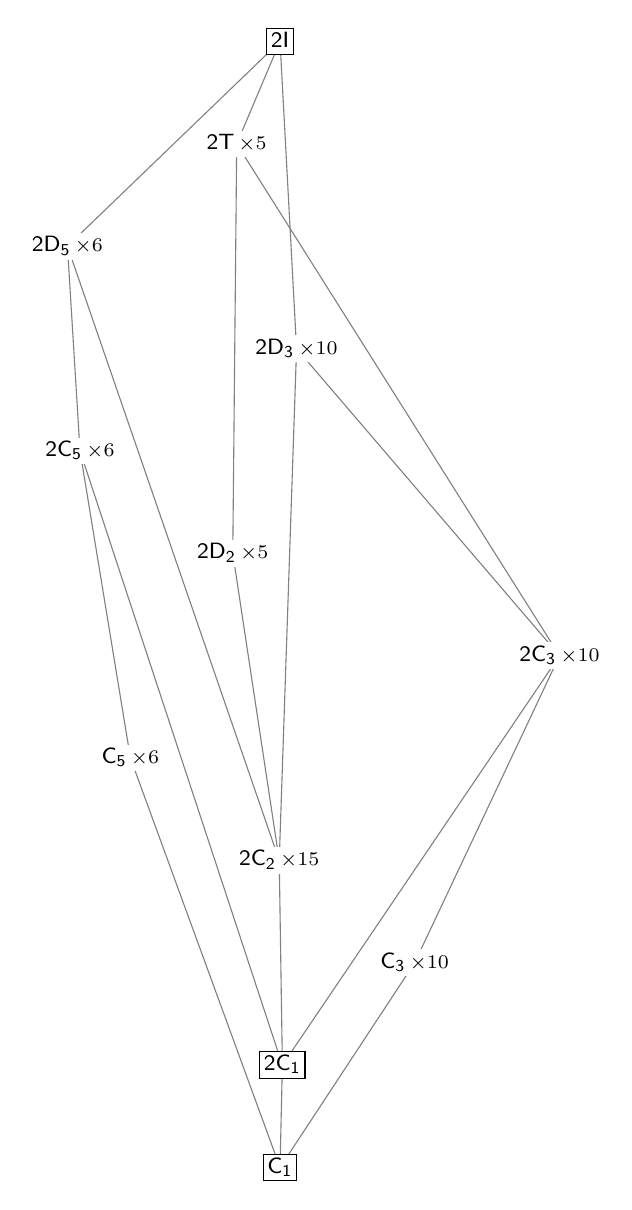
\begin{tikzpicture}[x=1cm, y=1.300cm,
  every node/.style={fill=white, font=\footnotesize, inner xsep=1.5pt, inner ysep=1.2pt, text height=5.6pt, text depth=1.6pt},
  normal/.style={draw, line width=0.4pt}, cover/.style={black!50, line width=0.4pt}]
\draw[cover] (0.00,0) -- (0.03,1);
\draw[cover] (0.00,0) -- (1.71,2);
\draw[cover] (0.00,0) -- (-1.90,4);
\draw[cover] (0.03,1) -- (-0.01,3);
\draw[cover] (0.03,1) -- (3.55,5);
\draw[cover] (0.03,1) -- (-2.54,7);
\draw[cover] (1.71,2) -- (3.55,5);
\draw[cover] (-0.01,3) -- (-0.60,6);
\draw[cover] (-0.01,3) -- (0.21,8);
\draw[cover] (-0.01,3) -- (-2.70,9);
\draw[cover] (-1.90,4) -- (-2.54,7);
\draw[cover] (3.55,5) -- (0.21,8);
\draw[cover] (3.55,5) -- (-0.55,10);
\draw[cover] (-0.60,6) -- (-0.55,10);
\draw[cover] (-2.54,7) -- (-2.70,9);
\draw[cover] (0.21,8) -- (0.00,11);
\draw[cover] (-2.70,9) -- (0.00,11);
\draw[cover] (-0.55,10) -- (0.00,11);
\node[normal] (n00) at (0.00,0) {$\grp{C_{1}}$};
\node[normal] (n01) at (0.03,1) {$\grp{2C_{1}}$};
\node (n02) at (1.71,2) {$\grp{C_{3}}$\,\nconj{10}};
\node (n03) at (-0.01,3) {$\grp{2C_{2}}$\,\nconj{15}};
\node (n04) at (-1.90,4) {$\grp{C_{5}}$\,\nconj{6}};
\node (n05) at (3.55,5) {$\grp{2C_{3}}$\,\nconj{10}};
\node (n06) at (-0.60,6) {$\grp{2D_{2}}$\,\nconj{5}};
\node (n07) at (-2.54,7) {$\grp{2C_{5}}$\,\nconj{6}};
\node (n08) at (0.21,8) {$\grp{2D_{3}}$\,\nconj{10}};
\node (n09) at (-2.70,9) {$\grp{2D_{5}}$\,\nconj{6}};
\node (n10) at (-0.55,10) {$\grp{2T}$\,\nconj{5}};
\node[normal] (n11) at (0.00,11) {$\grp{2I}$};
\end{tikzpicture}
\end{center}
{\small\setlength{\fillwidth}{\textwidth}\addtolength{\fillwidth}{-12\tabcolsep}\setlength{\colwidth}{0pt}\cellmax{$\grp{2C_{2}}$ $\samecls$ $\grp{2D_{1}}$}\cellmax{subgrp}\cellmax{$\grp{2C_{1}}$}\cellmax{$\grp{2C_{3}}$}\cellmax{$\grp{2C_{5}}$}\cellmax{$\grp{2D_{2}}$}\cellmax{$\grp{2D_{3}}$}\cellmax{$\grp{2D_{5}}$}\cellmax{$\grp{2I}$}\cellmax{$\grp{2T}$}\cellmax{$\grp{C_{1}}$}\cellmax{$\grp{C_{3}}$}\cellmax{$\grp{C_{5}}$}\addtolength{\fillwidth}{-\colwidth}\setlength{\colwidth}{0pt}\cellmax{order}\cellmax{120}\cellmax{10}\cellmax{12}\cellmax{20}\cellmax{24}\cellmax{1}\cellmax{2}\cellmax{3}\cellmax{4}\cellmax{5}\cellmax{6}\cellmax{8}\addtolength{\fillwidth}{-\colwidth}\setlength{\colwidth}{0pt}\cellmax{conjugates}\cellmax{10}\cellmax{15}\cellmax{1}\cellmax{5}\cellmax{6}\addtolength{\fillwidth}{-\colwidth}\setlength{\colwidth}{0pt}\cellmax{normal}\cellmax{yes}\cellmax{no}\addtolength{\fillwidth}{-\colwidth}\setlength{\colwidth}{0pt}\cellmax{$\grp{N}_{\hairsp \grp{2I}}(\grp{H})$}\cellmax{$\grp{2D_{2}}$}\cellmax{$\grp{2D_{3}}$}\cellmax{$\grp{2D_{5}}$}\cellmax{$\grp{2I}$}\cellmax{$\grp{2T}$}\addtolength{\fillwidth}{-\colwidth}\setlength{\colwidth}{0pt}\cellmax{$\grp{C}_{\hairsp \grp{2I}}(\grp{H})$}\cellmax{$\grp{2C_{1}}$}\cellmax{$\grp{2C_{2}}$}\cellmax{$\grp{2C_{3}}$}\cellmax{$\grp{2C_{5}}$}\cellmax{$\grp{2I}$}\addtolength{\fillwidth}{-\colwidth}\setlength{\colwidth}{0pt}\cellmax{$\cls{\barred{E}}$, $\cls{12C_{5}}$, $\cls{12\barred{C}_{5}}$, $\cls{12C_{5}^{2}}$, $\cls{12\barred{C}_{5}^{2}}$, $\cls{30C_{2}}$}\cellmax{$\cls{\barred{E}}$, $\cls{12C_{5}}$, $\cls{12\barred{C}_{5}}$, $\cls{12C_{5}^{2}}$, $\cls{12\barred{C}_{5}^{2}}$}\cellmax{$\cls{\barred{E}}$, $\cls{20C_{3}}$, $\cls{20\barred{C}_{3}}$, $\cls{30C_{2}}$}\cellmax{$\cls{\barred{E}}$, $\cls{20C_{3}}$, $\cls{20\barred{C}_{3}}$}\cellmax{$\cls{12\barred{C}_{5}}$, $\cls{12C_{5}^{2}}$}\cellmax{$\cls{\barred{E}}$, $\cls{30C_{2}}$}\cellmax{classes}\cellmax{$\cls{20\barred{C}_{3}}$}\cellmax{---}\cellmax{all}\cellmax{$\cls{\barred{E}}$}\fillcap\begin{longtable}{@{}lrrlll>{\RaggedRight\arraybackslash}p{\fillwidth}@{}}\toprule
subgrp & order & conjugates & normal & $\grp{N}_{\hairsp \grp{2I}}(\grp{H})$ & $\grp{C}_{\hairsp \grp{2I}}(\grp{H})$ & classes\\\midrule\endhead
\bottomrule\endfoot\endlastfoot
\href{C1.pdf}{$\grp{C_{1}}$} & 1 & 1 & yes & \href{2I.pdf}{$\grp{2I}$} & \href{2I.pdf}{$\grp{2I}$} & ---\\*
\href{2C1.pdf}{$\grp{2C_{1}}$} & 2 & 1 & yes & \href{2I.pdf}{$\grp{2I}$} & \href{2I.pdf}{$\grp{2I}$} & $\cls{\barred{E}}$\\
\href{C3.pdf}{$\grp{C_{3}}$} & 3 & 10 & no & \href{2D3.pdf}{$\grp{2D_{3}}$} & \href{2C3.pdf}{$\grp{2C_{3}}$} & $\cls{20\barred{C}_{3}}$\\
\href{2C2.pdf}{$\grp{2C_{2}}$} $\samecls$ \href{2D1.pdf}{$\grp{2D_{1}}$} & 4 & 15 & no & \href{2D2.pdf}{$\grp{2D_{2}}$} & \href{2C2.pdf}{$\grp{2C_{2}}$} & $\cls{\barred{E}}$, $\cls{30C_{2}}$\\
\href{C5.pdf}{$\grp{C_{5}}$} & 5 & 6 & no & \href{2D5.pdf}{$\grp{2D_{5}}$} & \href{2C5.pdf}{$\grp{2C_{5}}$} & $\cls{12\barred{C}_{5}}$, $\cls{12C_{5}^{2}}$\\
\href{2C3.pdf}{$\grp{2C_{3}}$} & 6 & 10 & no & \href{2D3.pdf}{$\grp{2D_{3}}$} & \href{2C3.pdf}{$\grp{2C_{3}}$} & $\cls{\barred{E}}$, $\cls{20C_{3}}$, $\cls{20\barred{C}_{3}}$\\
\href{2D2.pdf}{$\grp{2D_{2}}$} & 8 & 5 & no & \href{2T.pdf}{$\grp{2T}$} & \href{2C1.pdf}{$\grp{2C_{1}}$} & $\cls{\barred{E}}$, $\cls{30C_{2}}$\\
\href{2C5.pdf}{$\grp{2C_{5}}$} & 10 & 6 & no & \href{2D5.pdf}{$\grp{2D_{5}}$} & \href{2C5.pdf}{$\grp{2C_{5}}$} & $\cls{\barred{E}}$, $\cls{12C_{5}}$, $\cls{12\barred{C}_{5}}$, $\cls{12C_{5}^{2}}$, $\cls{12\barred{C}_{5}^{2}}$\\
\href{2D3.pdf}{$\grp{2D_{3}}$} & 12 & 10 & no & \href{2D3.pdf}{$\grp{2D_{3}}$} & \href{2C1.pdf}{$\grp{2C_{1}}$} & $\cls{\barred{E}}$, $\cls{20C_{3}}$, $\cls{20\barred{C}_{3}}$, $\cls{30C_{2}}$\\
\href{2D5.pdf}{$\grp{2D_{5}}$} & 20 & 6 & no & \href{2D5.pdf}{$\grp{2D_{5}}$} & \href{2C1.pdf}{$\grp{2C_{1}}$} & $\cls{\barred{E}}$, $\cls{12C_{5}}$, $\cls{12\barred{C}_{5}}$, $\cls{12C_{5}^{2}}$, $\cls{12\barred{C}_{5}^{2}}$, $\cls{30C_{2}}$\\
\href{2T.pdf}{$\grp{2T}$} & 24 & 5 & no & \href{2T.pdf}{$\grp{2T}$} & \href{2C1.pdf}{$\grp{2C_{1}}$} & $\cls{\barred{E}}$, $\cls{20C_{3}}$, $\cls{20\barred{C}_{3}}$, $\cls{30C_{2}}$\\*
\href{2I.pdf}{$\grp{2I}$} & 120 & 1 & yes & \href{2I.pdf}{$\grp{2I}$} & \href{2C1.pdf}{$\grp{2C_{1}}$} & all\\
\bottomrule\end{longtable}}
\needspace{103pt}
\section{Descent of symmetry}\label{s:subduction}
Conventions: \href{../../CONVENTIONS.pdf}{CONVENTIONS.pdf}, sections \href{../../../rotation/CONVENTIONS.pdf\#conv.12.2}{12.2}, \href{../../../rotation/CONVENTIONS.pdf\#conv.12.4}{12.4} and \href{../../CONVENTIONS.pdf\#conv.28}{28}.
A column is a class of subgroups $\grp{H}$, in the order of the table of section~\ref{s:subgroups}, by its symbol in the row subgrp as there, with the letter that tells apart classes with the same symbol, which are not conjugate in $\grp{2I}$; the symbol links to the document of $\grp{H}$. The entry of row $\Gamma$ is $\restr{\Gamma}{\grp{H}}$, the restriction of $\Gamma$ along a monomorphism from the record of $\grp{H}$ onto the subgroup, as a sum of the irreps of $\grp{H}$; the monomorphism identifies the subgroup with its record, and $\grp{H}$ names both. The rows of the vector irreps of a preimage are those of \href{../../../rotation/data/pdf/I.pdf}{$\grp{I}$} (\texttt{vector\symbol{95}subduction}); the column of a section is that of its preimage with the spinor irreps renamed (\href{../../CONVENTIONS.pdf}{CONVENTIONS.pdf}, section \href{../../CONVENTIONS.pdf\#conv.27}{27}), which the record does not store.
{\small\begin{longtable}{@{}lcccc@{}}\toprule
subgrp & \href{2C1.pdf}{$\grp{2C_{1}}$} & \href{C3.pdf}{$\grp{C_{3}}$} & \href{2C2.pdf}{$\grp{2C_{2}}$} & \href{C5.pdf}{$\grp{C_{5}}$}\\\midrule\endhead
\bottomrule\endfoot\endlastfoot
$\irr{a}$ & $\irr{a}$ & $\irr{a}$ & $\irr{a}$ & $\irr{a}$\\*
$\irr{t}_{1}$ & $3\,\irr{a}$ & $\irr{a}\oplus \conjpair{1}\irr{e}\oplus \conjpair{2}\irr{e}$ & $\irr{a}\oplus 2\,\irr{b}$ & $\irr{a}\oplus \conjpair{1}\irr{e}_{1}\oplus \conjpair{2}\irr{e}_{1}$\\*
$\irr{t}_{2}$ & $3\,\irr{a}$ & $\irr{a}\oplus \conjpair{1}\irr{e}\oplus \conjpair{2}\irr{e}$ & $\irr{a}\oplus 2\,\irr{b}$ & $\irr{a}\oplus \conjpair{1}\irr{e}_{2}\oplus \conjpair{2}\irr{e}_{2}$\\*
$\irr{g}$ & $4\,\irr{a}$ & $2\,\irr{a}\oplus \conjpair{1}\irr{e}\oplus \conjpair{2}\irr{e}$ & $2\,\irr{a}\oplus 2\,\irr{b}$ & $\conjpair{1}\irr{e}_{1}\oplus \conjpair{2}\irr{e}_{1}\oplus \conjpair{1}\irr{e}_{2}\oplus \conjpair{2}\irr{e}_{2}$\\*
$\irr{h}$ & $5\,\irr{a}$ & $\irr{a}\oplus 2\,\conjpair{1}\irr{e}\oplus 2\,\conjpair{2}\irr{e}$ & $3\,\irr{a}\oplus 2\,\irr{b}$ & $\irr{a}\oplus \conjpair{1}\irr{e}_{1}\oplus \conjpair{2}\irr{e}_{1}\oplus \conjpair{1}\irr{e}_{2}\oplus \conjpair{2}\irr{e}_{2}$\\*
$\irr{e}_{1/2}$ & $2\,\irr{a}_{1/2}$ & $\conjpair{2}\irr{e}\oplus \conjpair{1}\irr{e}$ & $\conjpair{1}\irr{e}_{1/2}\oplus \conjpair{2}\irr{e}_{1/2}$ & $\conjpair{2}\irr{e}_{2}\oplus \conjpair{1}\irr{e}_{2}$\\*
$\irr{e}_{7/2}$ & $2\,\irr{a}_{1/2}$ & $\conjpair{2}\irr{e}\oplus \conjpair{1}\irr{e}$ & $\conjpair{1}\irr{e}_{1/2}\oplus \conjpair{2}\irr{e}_{1/2}$ & $\conjpair{2}\irr{e}_{1}\oplus \conjpair{1}\irr{e}_{1}$\\*
$\irr{g}_{3/2}$ & $4\,\irr{a}_{1/2}$ & $2\,\irr{a}\oplus \conjpair{2}\irr{e}\oplus \conjpair{1}\irr{e}$ & $2\,\conjpair{1}\irr{e}_{1/2}\oplus 2\,\conjpair{2}\irr{e}_{1/2}$ & $\conjpair{2}\irr{e}_{2}\oplus \conjpair{1}\irr{e}_{2}\oplus \conjpair{2}\irr{e}_{1}\oplus \conjpair{1}\irr{e}_{1}$\\*
$\irr{i}_{5/2}$ & $6\,\irr{a}_{1/2}$ & $2\,\irr{a}\oplus 2\,\conjpair{2}\irr{e}\oplus 2\,\conjpair{1}\irr{e}$ & $3\,\conjpair{1}\irr{e}_{1/2}\oplus 3\,\conjpair{2}\irr{e}_{1/2}$ & $2\,\irr{a}\oplus \conjpair{2}\irr{e}_{2}\oplus \conjpair{1}\irr{e}_{2}\oplus \conjpair{2}\irr{e}_{1}\oplus \conjpair{1}\irr{e}_{1}$\\
\bottomrule\end{longtable}}
{\small\begin{longtable}{@{}lccc@{}}\toprule
subgrp & \href{2C3.pdf}{$\grp{2C_{3}}$} & \href{2D2.pdf}{$\grp{2D_{2}}$} & \href{2C5.pdf}{$\grp{2C_{5}}$}\\\midrule\endhead
\bottomrule\endfoot\endlastfoot
$\irr{a}$ & $\irr{a}$ & $\irr{a}$ & $\irr{a}$\\*
$\irr{t}_{1}$ & $\irr{a}\oplus \conjpair{1}\irr{e}\oplus \conjpair{2}\irr{e}$ & $\irr{b}_{1}\oplus \irr{b}_{2}\oplus \irr{b}_{3}$ & $\irr{a}\oplus \conjpair{1}\irr{e}_{1}\oplus \conjpair{2}\irr{e}_{1}$\\*
$\irr{t}_{2}$ & $\irr{a}\oplus \conjpair{1}\irr{e}\oplus \conjpair{2}\irr{e}$ & $\irr{b}_{1}\oplus \irr{b}_{2}\oplus \irr{b}_{3}$ & $\irr{a}\oplus \conjpair{1}\irr{e}_{2}\oplus \conjpair{2}\irr{e}_{2}$\\*
$\irr{g}$ & $2\,\irr{a}\oplus \conjpair{1}\irr{e}\oplus \conjpair{2}\irr{e}$ & $\irr{a}\oplus \irr{b}_{1}\oplus \irr{b}_{2}\oplus \irr{b}_{3}$ & $\conjpair{1}\irr{e}_{1}\oplus \conjpair{2}\irr{e}_{1}\oplus \conjpair{1}\irr{e}_{2}\oplus \conjpair{2}\irr{e}_{2}$\\*
$\irr{h}$ & $\irr{a}\oplus 2\,\conjpair{1}\irr{e}\oplus 2\,\conjpair{2}\irr{e}$ & $2\,\irr{a}\oplus \irr{b}_{1}\oplus \irr{b}_{2}\oplus \irr{b}_{3}$ & $\irr{a}\oplus \conjpair{1}\irr{e}_{1}\oplus \conjpair{2}\irr{e}_{1}\oplus \conjpair{1}\irr{e}_{2}\oplus \conjpair{2}\irr{e}_{2}$\\*
$\irr{e}_{1/2}$ & $\conjpair{1}\irr{e}_{1/2}\oplus \conjpair{2}\irr{e}_{1/2}$ & $\irr{e}_{1/2}$ & $\conjpair{1}\irr{e}_{1/2}\oplus \conjpair{2}\irr{e}_{1/2}$\\*
$\irr{e}_{7/2}$ & $\conjpair{1}\irr{e}_{1/2}\oplus \conjpair{2}\irr{e}_{1/2}$ & $\irr{e}_{1/2}$ & $\conjpair{1}\irr{e}_{3/2}\oplus \conjpair{2}\irr{e}_{3/2}$\\*
$\irr{g}_{3/2}$ & $2\,\irr{a}_{3/2}\oplus \conjpair{1}\irr{e}_{1/2}\oplus \conjpair{2}\irr{e}_{1/2}$ & $2\,\irr{e}_{1/2}$ & $\conjpair{1}\irr{e}_{1/2}\oplus \conjpair{2}\irr{e}_{1/2}\oplus \conjpair{1}\irr{e}_{3/2}\oplus \conjpair{2}\irr{e}_{3/2}$\\*
$\irr{i}_{5/2}$ & $2\,\irr{a}_{3/2}\oplus 2\,\conjpair{1}\irr{e}_{1/2}\oplus 2\,\conjpair{2}\irr{e}_{1/2}$ & $3\,\irr{e}_{1/2}$ & $2\,\irr{a}_{5/2}\oplus \conjpair{1}\irr{e}_{1/2}\oplus \conjpair{2}\irr{e}_{1/2}\oplus \conjpair{1}\irr{e}_{3/2}\oplus \conjpair{2}\irr{e}_{3/2}$\\
\bottomrule\end{longtable}}
{\small\begin{longtable}{@{}lccc@{}}\toprule
subgrp & \href{2D3.pdf}{$\grp{2D_{3}}$} & \href{2D5.pdf}{$\grp{2D_{5}}$} & \href{2T.pdf}{$\grp{2T}$}\\\midrule\endhead
\bottomrule\endfoot\endlastfoot
$\irr{a}$ & $\irr{a}_{1}$ & $\irr{a}_{1}$ & $\irr{a}$\\*
$\irr{t}_{1}$ & $\irr{a}_{2}\oplus \irr{e}$ & $\irr{a}_{2}\oplus \irr{e}_{1}$ & $\irr{t}$\\*
$\irr{t}_{2}$ & $\irr{a}_{2}\oplus \irr{e}$ & $\irr{a}_{2}\oplus \irr{e}_{2}$ & $\irr{t}$\\*
$\irr{g}$ & $\irr{a}_{1}\oplus \irr{a}_{2}\oplus \irr{e}$ & $\irr{e}_{1}\oplus \irr{e}_{2}$ & $\irr{a}\oplus \irr{t}$\\*
$\irr{h}$ & $\irr{a}_{1}\oplus 2\,\irr{e}$ & $\irr{a}_{1}\oplus \irr{e}_{1}\oplus \irr{e}_{2}$ & $\conjpair{1}\irr{e}\oplus \conjpair{2}\irr{e}\oplus \irr{t}$\\*
$\irr{e}_{1/2}$ & $\irr{e}_{1/2}$ & $\irr{e}_{1/2}$ & $\irr{e}_{1/2}$\\*
$\irr{e}_{7/2}$ & $\irr{e}_{1/2}$ & $\irr{e}_{3/2}$ & $\irr{e}_{1/2}$\\*
$\irr{g}_{3/2}$ & $\irr{e}_{1/2}\oplus \conjpair{1}\irr{e}_{3/2}\oplus \conjpair{2}\irr{e}_{3/2}$ & $\irr{e}_{1/2}\oplus \irr{e}_{3/2}$ & $\conjpair{1}\irr{g}_{3/2}\oplus \conjpair{2}\irr{g}_{3/2}$\\*
$\irr{i}_{5/2}$ & $2\,\irr{e}_{1/2}\oplus \conjpair{1}\irr{e}_{3/2}\oplus \conjpair{2}\irr{e}_{3/2}$ & $\irr{e}_{1/2}\oplus \irr{e}_{3/2}\oplus \conjpair{1}\irr{e}_{5/2}\oplus \conjpair{2}\irr{e}_{5/2}$ & $\irr{e}_{1/2}\oplus \conjpair{1}\irr{g}_{3/2}\oplus \conjpair{2}\irr{g}_{3/2}$\\
\bottomrule\end{longtable}}
\leavevmode\label{n:irrep.Delta}Read down a column, a table gives induction (Frobenius reciprocity): $\Gamma$ occurs in $\Ind{\grp{H}}{\grp{2I}} \Lambda$ as often as $\Lambda$ occurs in the entry of row $\Gamma$. The JSON gives, for every entry of a spinor irrep, the unitary matrix that carries $\restr{\Gamma}{\grp{H}}$ into the direct sum of the matrices of $\grp{H}$ (\texttt{subduction[].blocks}), and for every class the left coset representatives of $\grp{H}$ (\texttt{transversal}), from which \href{../../CONVENTIONS.pdf}{CONVENTIONS.pdf}, section \href{../../../rotation/CONVENTIONS.pdf\#conv.12.4}{12.4}, builds $\Ind{\grp{H}}{\grp{2I}} \Lambda$ and its intertwiners.
\needspace{190pt}
\partbox{Angular momentum}
\section{Subduction from \texorpdfstring{$\grp{Pin^{-}(3)}$}{Pin\unichar{8315}(3)}}\label{s:subduction_parent}
Conventions: \href{../../CONVENTIONS.pdf}{CONVENTIONS.pdf}, sections \href{../../../rotation/CONVENTIONS.pdf\#conv.11}{11} and \href{../../CONVENTIONS.pdf\#conv.25.1}{25.1}.
\leavevmode\label{n:index.J}\label{n:index.parity}\label{n:irrep.o3}\label{n:function.character.parent}\label{n:function.multiplicity}$\irrJp{J}{p}$ is the irrep of $\grp{Pin^{-}(3)}$ of angular momentum $J$ ($J = 0, \nicefrac{1}{2}, 1, \dots$) and parity $p = \pm 1$, on which $(U, \varepsilon)$ acts as $\varepsilon^{[p = -1]}$ times $U$ acting on the kets of angular momentum $J$; $\elt{\barred{E}}$ acts as $(-1)^{2J}$. An element whose $\grp{SU(2)}$ part is $\lift{R}_{\vv}(\omega)$ (section~\ref{s:elements}) has the character
\begin{equation}\label{e:chi}\chi^{(J,p)}(g) = p^{\iverson{\det g = -1}}\sum_{m=-J}^{J} \expe^{\iunit m\omega},\end{equation}
and $b_\Gamma(J, p)$ is the multiplicity of $\Gamma$ in
\begin{equation}\label{e:parent}\restr{\irrJp{J}{p}}{\grp{2I}}.\end{equation}
\leavevmode\label{n:index.increment}At integer $J$ only the vector irreps occur, and $b_\Gamma(J, p)$ is the multiplicity of the subduction from $\grp{O(3)}$ in \href{../../../rotation/data/pdf/I.pdf}{$\grp{I}$} (\texttt{integer\symbol{95}J}). At half-integer $J$ only the spinor irreps occur: each table gives $b_\Gamma(J, p)$ for $2J \le 41$, and $b_\Gamma(J + 15, p) = b_\Gamma(J, p) + \Delta_\Gamma$ for every $J$ of the table, $\Delta_\Gamma$ its last row. A table leaves out the irreps whose multiplicity is 0 for every $J$.
\needspace{194pt}
\paragraph{Half-integer $J$, $p = \pm 1$.}
The multiplicities do not depend on $p$, as every element of $\grp{2I}$ is a rotation: one table holds both parities.
{\small\begin{longtable}{@{}rrrrr@{\hspace{18pt}}rrrrr@{\hspace{18pt}}rrrrr@{}}\toprule
$J$ & $\irr{e}_{1/2}$ & $\irr{e}_{7/2}$ & $\irr{g}_{3/2}$ & $\irr{i}_{5/2}$ & $J$ & $\irr{e}_{1/2}$ & $\irr{e}_{7/2}$ & $\irr{g}_{3/2}$ & $\irr{i}_{5/2}$ & $J$ & $\irr{e}_{1/2}$ & $\irr{e}_{7/2}$ & $\irr{g}_{3/2}$ & $\irr{i}_{5/2}$\\\midrule\endhead
\bottomrule\endfoot\endlastfoot
$\nicefrac{1}{2}$ & 1 & 0 & 0 & 0 & $\nicefrac{17}{2}$ & 0 & 1 & 1 & 2 & $\nicefrac{33}{2}$ & 1 & 1 & 3 & 3\\*
$\nicefrac{3}{2}$ & 0 & 0 & 1 & 0 & $\nicefrac{19}{2}$ & 1 & 1 & 1 & 2 & $\nicefrac{35}{2}$ & 1 & 1 & 2 & 4\\*
$\nicefrac{5}{2}$ & 0 & 0 & 0 & 1 & $\nicefrac{21}{2}$ & 1 & 0 & 2 & 2 & $\nicefrac{37}{2}$ & 1 & 2 & 2 & 4\\*
$\nicefrac{7}{2}$ & 0 & 1 & 0 & 1 & $\nicefrac{23}{2}$ & 1 & 1 & 2 & 2 & $\nicefrac{39}{2}$ & 1 & 1 & 3 & 4\\*
$\nicefrac{9}{2}$ & 0 & 0 & 1 & 1 & $\nicefrac{25}{2}$ & 1 & 1 & 1 & 3 & $\nicefrac{41}{2}$ & 2 & 1 & 3 & 4\\*\noalign{\vskip 1.5pt}\multispan{5} & \multispan{5} & \multispan{5}\leaders\hrule height\cmidrulewidth\hfill\kern0pt\\*\noalign{\vskip 1.5pt}
$\nicefrac{11}{2}$ & 1 & 0 & 1 & 1 & $\nicefrac{27}{2}$ & 0 & 1 & 2 & 3 & $\Delta_\Gamma$ & 1 & 1 & 2 & 3\\*
$\nicefrac{13}{2}$ & 1 & 1 & 1 & 1 & $\nicefrac{29}{2}$ & 1 & 1 & 2 & 3 &  &  &  &  & \\*
$\nicefrac{15}{2}$ & 0 & 0 & 1 & 2 & $\nicefrac{31}{2}$ & 2 & 1 & 2 & 3 &  &  &  &  & \\
\bottomrule\end{longtable}}
\needspace{110pt}
\section{Multiplicities and allowed \texorpdfstring{$m$}{m}}\label{s:multiplicities}
Conventions: \href{../../CONVENTIONS.pdf}{CONVENTIONS.pdf}, sections \href{../../../rotation/CONVENTIONS.pdf\#conv.14}{14} and \href{../../CONVENTIONS.pdf\#conv.26}{26}.
\leavevmode\label{n:function.generating}\label{n:index.generating.variable}\label{n:function.generating.numerator}$b_\Gamma(J)$ is the number of blocks of $\Gamma$ at $J$, with the generating function
\begin{equation}\label{e:gf}H_\Gamma(t) = \sum_{J\ge1/2} b_\Gamma(J)\,t^{2J} = P_\Gamma(t)/((1-t^{10})(1-t^{12})),\end{equation}
the sum over the half-integer $J$. Every nonzero component of a vector of $\Gamma$ has $2m \bmod 4$ in the listed residues, and each listed residue occurs.
{\small\begin{longtable}{@{}lll@{}}\toprule
$\Gamma$ & $P_\Gamma(t)$ & $2m \bmod 4$\\\midrule\endhead
\bottomrule\endfoot\endlastfoot
$\irr{e}_{1/2}$ & $t + t^{19}$ & 1, 3\\*
$\irr{e}_{7/2}$ & $t^{7} + t^{13}$ & 1, 3\\*
$\irr{g}_{3/2}$ & $t^{3} + t^{9} + t^{11} + t^{17}$ & 1, 3\\*
$\irr{i}_{5/2}$ & $t^{5} + t^{7} + t^{9} + t^{11} + t^{13} + t^{15}$ & 1, 3\\
\bottomrule\end{longtable}}
\needspace{110pt}
\section{Symmetry-adapted bases}\label{s:bases}
Conventions: \href{../../CONVENTIONS.pdf}{CONVENTIONS.pdf}, sections \href{../../../rotation/CONVENTIONS.pdf\#conv.14}{14}, \href{../../../rotation/CONVENTIONS.pdf\#conv.14.2}{14.2} and \href{../../CONVENTIONS.pdf\#conv.26}{26}.
\leavevmode\label{n:index.m}\label{n:vector.ket}\label{n:index.ketcoefficient}\label{n:vector.basis.symmetry}\label{n:index.ketweight}\label{n:index.total}The bases at integer $J$ are those of \href{../../../rotation/data/pdf/I.pdf}{$\grp{I}$} (\texttt{integer\symbol{95}J}). At half-integer $J$ the kets $\jm{J}{m}$, $m = J, J-1, \dots, -J$, carry $\irrJp{J}{+1}$; the element $g$ of $\grp{2I}$ whose $\grp{SU(2)}$ part is $U$ acts as
\begin{equation}\label{e:action}g\,\jm{J}{m} = \sum_{m'} \jm{J}{m'}\; \conj{\wignerD{J}_{m m'}(U)},\end{equation}
\leavevmode\label{n:matrix.wigner}$\wignerD{J}$ the Wigner matrix of $\grp{SU(2)}$ ($\wignerD{1/2}(U) = U$ on $\jm{1/2}{1/2}$, $\jm{1/2}{-1/2}$). So $\lift{R}_{z}(\omega)$ multiplies $\jm{J}{m}$ by $\expe^{\iunit m\omega}$, $0 \le \omega < 4\pi$, and $\elt{\barred{E}}$ by $-1$. A vector is listed by its coefficients $e_m$:
\begin{equation}\label{e:ket}v = \frac{1}{\sqrt{\mathrm{tot}}}\sum_m e_m\sqrt{F_m}\;\jm{J}{m},\qquad F_m = (J+m)!\,(J-m)!,\qquad \mathrm{tot} = \sum_m |e_m|^2F_m;\end{equation}
\leavevmode\label{n:index.factor.c}the amplitude of $\jm{J}{m}$ is $e_m\sqrt{F_m/\mathrm{tot}}$, and a vector written $c\sum_m q_m\jm{J}{m}$ has $e_m = c\,q_m$.
\leavevmode\label{n:matrix.projector}The copies of $\Gamma$ at $J$ are orthonormal. Their partner-1 vectors are the vectors of the reduced echelon basis, in the coordinates $e_m$, $m = -J, -J+1, \dots, J$, of the range of
\begin{equation}\label{e:projector}P^\Gamma_{1,1} = \sum_g \conj{\repD{\Gamma}_{1,1}(g)}\,\irrJp{J}{+1}(g),\end{equation}
$\mult$ ascending with the lowest $m$ of each, each less its projections on the copies before it (Gram--Schmidt); partner $\intx$ is $P^\Gamma_{\intx,1}$ applied to partner 1.
\label{n:head.vector}31 blocks, 132 vectors, $J = \nicefrac{1}{2}, \nicefrac{3}{2}, \dots, \nicefrac{21}{2}$, in \texttt{data/symmetry\symbol{95}adapted\symbol{95}bases/2I/}; a row gives a vector of a block at $J$: the block's irrep and copy index $\mult$, the partner index $\intx$ and the vector; the full set $J \le \nicefrac{121}{2}$ (883 blocks, 3782 vectors) is in the same folder, $J \le \nicefrac{21}{2}$ in the repository and $J = \nicefrac{23}{2}, \nicefrac{25}{2}, \dots, \nicefrac{121}{2}$ in the release archive \texttt{2I\symbol{95}2J023-2J121.tar}, which unpacks in the folder \texttt{double/} (README.md).
{\small\setlength{\tabcolsep}{3pt}\setlength{\fillwidth}{\textwidth}\addtolength{\fillwidth}{-\dimexpr 6\tabcolsep+4pt\relax}\setlength{\colwidth}{0pt}\cellmax{11/2}\cellmax{13/2}\cellmax{15/2}\cellmax{17/2}\cellmax{19/2}\cellmax{21/2}\cellmax{1/2}\cellmax{3/2}\cellmax{5/2}\cellmax{7/2}\cellmax{9/2}\cellmax{$J$}\addtolength{\fillwidth}{-\colwidth}\setlength{\colwidth}{0pt}\cellmax{$\irr{e}_{1/2}$}\cellmax{$\irr{e}_{7/2}$}\cellmax{$\irr{g}_{3/2}$}\cellmax{$\irr{i}_{5/2}$}\cellmax{irrep}\addtolength{\fillwidth}{-\colwidth}\setlength{\colwidth}{0pt}\cellmax{$\mult$}\cellmax{1}\cellmax{2}\addtolength{\fillwidth}{-\colwidth}\setlength{\colwidth}{0pt}\cellmax{$\intx$}\cellmax{1}\cellmax{2}\cellmax{3}\cellmax{4}\cellmax{5}\cellmax{6}\addtolength{\fillwidth}{-\colwidth}\begin{longtable}{@{}rlrr@{\hspace{4pt}}>{\RaggedRight\arraybackslash}p{\fillwidth}@{}}\toprule
$J$ & irrep & $\mult$ & $\intx$ & vector\\\midrule\endhead
\bottomrule\endfoot\endlastfoot
$\nicefrac{1}{2}$ & $\irr{e}_{1/2}$ & 1 & 1 & $\jm{\nicefrac{1}{2}}{\nicefrac{1}{2}}$\\*
$\nicefrac{1}{2}$ & $\irr{e}_{1/2}$ & 1 & 2 & $\jm{\nicefrac{1}{2}}{-\nicefrac{1}{2}}$\\
\grouprule{0pt}{\lightrulewidth}
$\nicefrac{3}{2}$ & $\irr{g}_{3/2}$ & 1 & 1 & $\jm{\nicefrac{3}{2}}{\nicefrac{3}{2}}$\\*
$\nicefrac{3}{2}$ & $\irr{g}_{3/2}$ & 1 & 2 & $\sqrt{3}\,\jm{\nicefrac{3}{2}}{\nicefrac{1}{2}}$\\*
$\nicefrac{3}{2}$ & $\irr{g}_{3/2}$ & 1 & 3 & $\sqrt{3}\,\jm{\nicefrac{3}{2}}{-\nicefrac{1}{2}}$\\*
$\nicefrac{3}{2}$ & $\irr{g}_{3/2}$ & 1 & 4 & $\jm{\nicefrac{3}{2}}{-\nicefrac{3}{2}}$\\
\grouprule{0pt}{\lightrulewidth}
$\nicefrac{5}{2}$ & $\irr{i}_{5/2}$ & 1 & 1 & $\jm{\nicefrac{5}{2}}{\nicefrac{5}{2}}$\\*
$\nicefrac{5}{2}$ & $\irr{i}_{5/2}$ & 1 & 2 & $(2\goldenratio - 1)\,\jm{\nicefrac{5}{2}}{\nicefrac{3}{2}}$\\*
$\nicefrac{5}{2}$ & $\irr{i}_{5/2}$ & 1 & 3 & $\sqrt{10}\,\jm{\nicefrac{5}{2}}{\nicefrac{1}{2}}$\\*
$\nicefrac{5}{2}$ & $\irr{i}_{5/2}$ & 1 & 4 & $\sqrt{10}\,\jm{\nicefrac{5}{2}}{-\nicefrac{1}{2}}$\\*
$\nicefrac{5}{2}$ & $\irr{i}_{5/2}$ & 1 & 5 & $(2\goldenratio - 1)\,\jm{\nicefrac{5}{2}}{-\nicefrac{3}{2}}$\\*
$\nicefrac{5}{2}$ & $\irr{i}_{5/2}$ & 1 & 6 & $\jm{\nicefrac{5}{2}}{-\nicefrac{5}{2}}$\\
\grouprule{0pt}{\lightrulewidth}
$\nicefrac{7}{2}$ & $\irr{e}_{7/2}$ & 1 & 1 & $5\,\jm{\nicefrac{7}{2}}{-\nicefrac{7}{2}}$ $+$ $(7 - 14\goldenratio{})\,\jm{\nicefrac{7}{2}}{-\nicefrac{3}{2}}$ $+$ $35\,\jm{\nicefrac{7}{2}}{\nicefrac{1}{2}}$ $+$ $(14\goldenratio - 7)\,\jm{\nicefrac{7}{2}}{\nicefrac{5}{2}}$\\*
$\nicefrac{7}{2}$ & $\irr{e}_{7/2}$ & 1 & 2 & $(7 - 14\goldenratio{})\,\jm{\nicefrac{7}{2}}{-\nicefrac{5}{2}}$ $-35\,\jm{\nicefrac{7}{2}}{-\nicefrac{1}{2}}$ $+$ $(14\goldenratio - 7)\,\jm{\nicefrac{7}{2}}{\nicefrac{3}{2}}$ $-5\,\jm{\nicefrac{7}{2}}{\nicefrac{7}{2}}$\\
$\nicefrac{7}{2}$ & $\irr{i}_{5/2}$ & 1 & 1 & $15\,\jm{\nicefrac{7}{2}}{-\nicefrac{7}{2}}$ $+$ $(42\goldenratio - 21)\,\jm{\nicefrac{7}{2}}{-\nicefrac{3}{2}}$ $-35\,\jm{\nicefrac{7}{2}}{\nicefrac{1}{2}}$ $+$ $(1 - 2\goldenratio{})\,\jm{\nicefrac{7}{2}}{\nicefrac{5}{2}}$\\*
$\nicefrac{7}{2}$ & $\irr{i}_{5/2}$ & 1 & 2 & $-35\,\jm{\nicefrac{7}{2}}{-\nicefrac{5}{2}}$ $+$ $(70\goldenratio - 35)\,\jm{\nicefrac{7}{2}}{-\nicefrac{1}{2}}$ $+$ $15\,\jm{\nicefrac{7}{2}}{\nicefrac{3}{2}}$ $+$ $(2\goldenratio - 1)\,\jm{\nicefrac{7}{2}}{\nicefrac{7}{2}}$\\*
$\nicefrac{7}{2}$ & $\irr{i}_{5/2}$ & 1 & 3 & $5\sqrt{2}\,\jm{\nicefrac{7}{2}}{-\nicefrac{7}{2}}$ $-21\sqrt{10}\,\jm{\nicefrac{7}{2}}{-\nicefrac{3}{2}}$ $-25\sqrt{2}\,\jm{\nicefrac{7}{2}}{\nicefrac{1}{2}}$ $-7\sqrt{10}\,\jm{\nicefrac{7}{2}}{\nicefrac{5}{2}}$\\*
$\nicefrac{7}{2}$ & $\irr{i}_{5/2}$ & 1 & 4 & $7\sqrt{10}\,\jm{\nicefrac{7}{2}}{-\nicefrac{5}{2}}$ $+$ $25\sqrt{2}\,\jm{\nicefrac{7}{2}}{-\nicefrac{1}{2}}$ $+$ $21\sqrt{10}\,\jm{\nicefrac{7}{2}}{\nicefrac{3}{2}}$ $-5\sqrt{2}\,\jm{\nicefrac{7}{2}}{\nicefrac{7}{2}}$\\*
$\nicefrac{7}{2}$ & $\irr{i}_{5/2}$ & 1 & 5 & $(1 - 2\goldenratio{})\,\jm{\nicefrac{7}{2}}{-\nicefrac{7}{2}}$ $-15\,\jm{\nicefrac{7}{2}}{-\nicefrac{3}{2}}$ $+$ $(35 - 70\goldenratio{})\,\jm{\nicefrac{7}{2}}{\nicefrac{1}{2}}$ $+$ $35\,\jm{\nicefrac{7}{2}}{\nicefrac{5}{2}}$\\*
$\nicefrac{7}{2}$ & $\irr{i}_{5/2}$ & 1 & 6 & $(2\goldenratio - 1)\,\jm{\nicefrac{7}{2}}{-\nicefrac{5}{2}}$ $+$ $35\,\jm{\nicefrac{7}{2}}{-\nicefrac{1}{2}}$ $+$ $(21 - 42\goldenratio{})\,\jm{\nicefrac{7}{2}}{\nicefrac{3}{2}}$ $-15\,\jm{\nicefrac{7}{2}}{\nicefrac{7}{2}}$\\
\grouprule{0pt}{\lightrulewidth}
$\nicefrac{9}{2}$ & $\irr{g}_{3/2}$ & 1 & 1 & $5\,\jm{\nicefrac{9}{2}}{-\nicefrac{9}{2}}$ $+$ $(24\goldenratio - 12)\,\jm{\nicefrac{9}{2}}{-\nicefrac{5}{2}}$ $-42\,\jm{\nicefrac{9}{2}}{-\nicefrac{1}{2}}$ $+$ $(4 - 8\goldenratio{})\,\jm{\nicefrac{9}{2}}{\nicefrac{3}{2}}$ $-3\,\jm{\nicefrac{9}{2}}{\nicefrac{7}{2}}$\\*
$\nicefrac{9}{2}$ & $\irr{g}_{3/2}$ & 1 & 2 & $-9\sqrt{15}\,\jm{\nicefrac{9}{2}}{-\nicefrac{7}{2}}$ $+$ $84\sqrt{3}\,\jm{\nicefrac{9}{2}}{-\nicefrac{3}{2}}$ $+$ $18\sqrt{15}\,\jm{\nicefrac{9}{2}}{\nicefrac{1}{2}}$ $+$ $36\sqrt{3}\,\jm{\nicefrac{9}{2}}{\nicefrac{5}{2}}$ $-\sqrt{15}\,\jm{\nicefrac{9}{2}}{\nicefrac{9}{2}}$\\*
$\nicefrac{9}{2}$ & $\irr{g}_{3/2}$ & 1 & 3 & $\sqrt{15}\,\jm{\nicefrac{9}{2}}{-\nicefrac{9}{2}}$ $-36\sqrt{3}\,\jm{\nicefrac{9}{2}}{-\nicefrac{5}{2}}$ $-18\sqrt{15}\,\jm{\nicefrac{9}{2}}{-\nicefrac{1}{2}}$ $-84\sqrt{3}\,\jm{\nicefrac{9}{2}}{\nicefrac{3}{2}}$ $+$ $9\sqrt{15}\,\jm{\nicefrac{9}{2}}{\nicefrac{7}{2}}$\\*
$\nicefrac{9}{2}$ & $\irr{g}_{3/2}$ & 1 & 4 & $3\,\jm{\nicefrac{9}{2}}{-\nicefrac{7}{2}}$ $+$ $(8\goldenratio - 4)\,\jm{\nicefrac{9}{2}}{-\nicefrac{3}{2}}$ $+$ $42\,\jm{\nicefrac{9}{2}}{\nicefrac{1}{2}}$ $+$ $(12 - 24\goldenratio{})\,\jm{\nicefrac{9}{2}}{\nicefrac{5}{2}}$ $-5\,\jm{\nicefrac{9}{2}}{\nicefrac{9}{2}}$\\
$\nicefrac{9}{2}$ & $\irr{i}_{5/2}$ & 1 & 1 & $15\,\jm{\nicefrac{9}{2}}{-\nicefrac{7}{2}}$ $+$ $(56\goldenratio - 28)\,\jm{\nicefrac{9}{2}}{-\nicefrac{3}{2}}$ $-70\,\jm{\nicefrac{9}{2}}{\nicefrac{1}{2}}$ $+$ $(4 - 8\goldenratio{})\,\jm{\nicefrac{9}{2}}{\nicefrac{5}{2}}$ $-\jm{\nicefrac{9}{2}}{\nicefrac{9}{2}}$\\*
$\nicefrac{9}{2}$ & $\irr{i}_{5/2}$ & 1 & 2 & $(30\goldenratio - 15)\,\jm{\nicefrac{9}{2}}{-\nicefrac{9}{2}}$ $-20\,\jm{\nicefrac{9}{2}}{-\nicefrac{5}{2}}$ $+$ $(308\goldenratio - 154)\,\jm{\nicefrac{9}{2}}{-\nicefrac{1}{2}}$ $+$ $140\,\jm{\nicefrac{9}{2}}{\nicefrac{3}{2}}$ $+$ $(62\goldenratio - 31)\,\jm{\nicefrac{9}{2}}{\nicefrac{7}{2}}$\\*
$\nicefrac{9}{2}$ & $\irr{i}_{5/2}$ & 1 & 3 & $-65\sqrt{2}\,\jm{\nicefrac{9}{2}}{-\nicefrac{7}{2}}$ $+$ $28\sqrt{10}\,\jm{\nicefrac{9}{2}}{-\nicefrac{3}{2}}$ $-70\sqrt{2}\,\jm{\nicefrac{9}{2}}{\nicefrac{1}{2}}$ $-68\sqrt{10}\,\jm{\nicefrac{9}{2}}{\nicefrac{5}{2}}$ $+$ $15\sqrt{2}\,\jm{\nicefrac{9}{2}}{\nicefrac{9}{2}}$\\*
$\nicefrac{9}{2}$ & $\irr{i}_{5/2}$ & 1 & 4 & $15\sqrt{2}\,\jm{\nicefrac{9}{2}}{-\nicefrac{9}{2}}$ $-68\sqrt{10}\,\jm{\nicefrac{9}{2}}{-\nicefrac{5}{2}}$ $-70\sqrt{2}\,\jm{\nicefrac{9}{2}}{-\nicefrac{1}{2}}$ $+$ $28\sqrt{10}\,\jm{\nicefrac{9}{2}}{\nicefrac{3}{2}}$ $-65\sqrt{2}\,\jm{\nicefrac{9}{2}}{\nicefrac{7}{2}}$\\*
$\nicefrac{9}{2}$ & $\irr{i}_{5/2}$ & 1 & 5 & $(62\goldenratio - 31)\,\jm{\nicefrac{9}{2}}{-\nicefrac{7}{2}}$ $+$ $140\,\jm{\nicefrac{9}{2}}{-\nicefrac{3}{2}}$ $+$ $(308\goldenratio - 154)\,\jm{\nicefrac{9}{2}}{\nicefrac{1}{2}}$ $-20\,\jm{\nicefrac{9}{2}}{\nicefrac{5}{2}}$ $+$ $(30\goldenratio - 15)\,\jm{\nicefrac{9}{2}}{\nicefrac{9}{2}}$\\*
$\nicefrac{9}{2}$ & $\irr{i}_{5/2}$ & 1 & 6 & $-\jm{\nicefrac{9}{2}}{-\nicefrac{9}{2}}$ $+$ $(4 - 8\goldenratio{})\,\jm{\nicefrac{9}{2}}{-\nicefrac{5}{2}}$ $-70\,\jm{\nicefrac{9}{2}}{-\nicefrac{1}{2}}$ $+$ $(56\goldenratio - 28)\,\jm{\nicefrac{9}{2}}{\nicefrac{3}{2}}$ $+$ $15\,\jm{\nicefrac{9}{2}}{\nicefrac{7}{2}}$\\
\grouprule{0pt}{\lightrulewidth}
$\nicefrac{11}{2}$ & $\irr{e}_{1/2}$ & 1 & 1 & $15\,\jm{\nicefrac{11}{2}}{-\nicefrac{11}{2}}$ $+$ $(110\goldenratio - 55)\,\jm{\nicefrac{11}{2}}{-\nicefrac{7}{2}}$ $-330\,\jm{\nicefrac{11}{2}}{-\nicefrac{3}{2}}$ $+$ $(66 - 132\goldenratio{})\,\jm{\nicefrac{11}{2}}{\nicefrac{1}{2}}$ $-165\,\jm{\nicefrac{11}{2}}{\nicefrac{5}{2}}$ $+$ $(22\goldenratio - 11)\,\jm{\nicefrac{11}{2}}{\nicefrac{9}{2}}$\\*
$\nicefrac{11}{2}$ & $\irr{e}_{1/2}$ & 1 & 2 & $(11 - 22\goldenratio{})\,\jm{\nicefrac{11}{2}}{-\nicefrac{9}{2}}$ $+$ $165\,\jm{\nicefrac{11}{2}}{-\nicefrac{5}{2}}$ $+$ $(132\goldenratio - 66)\,\jm{\nicefrac{11}{2}}{-\nicefrac{1}{2}}$ $+$ $330\,\jm{\nicefrac{11}{2}}{\nicefrac{3}{2}}$ $+$ $(55 - 110\goldenratio{})\,\jm{\nicefrac{11}{2}}{\nicefrac{7}{2}}$ $-15\,\jm{\nicefrac{11}{2}}{\nicefrac{11}{2}}$\\
$\nicefrac{11}{2}$ & $\irr{g}_{3/2}$ & 1 & 1 & $15\,\jm{\nicefrac{11}{2}}{-\nicefrac{9}{2}}$ $+$ $(90\goldenratio - 45)\,\jm{\nicefrac{11}{2}}{-\nicefrac{5}{2}}$ $-210\,\jm{\nicefrac{11}{2}}{-\nicefrac{1}{2}}$ $+$ $(30 - 60\goldenratio{})\,\jm{\nicefrac{11}{2}}{\nicefrac{3}{2}}$ $-45\,\jm{\nicefrac{11}{2}}{\nicefrac{7}{2}}$ $+$ $(2\goldenratio - 1)\,\jm{\nicefrac{11}{2}}{\nicefrac{11}{2}}$\\*
$\nicefrac{11}{2}$ & $\irr{g}_{3/2}$ & 1 & 2 & $15\sqrt{3}\,\jm{\nicefrac{11}{2}}{-\nicefrac{11}{2}}$ $+$ $25\sqrt{15}\,\jm{\nicefrac{11}{2}}{-\nicefrac{7}{2}}$ $+$ $30\sqrt{3}\,\jm{\nicefrac{11}{2}}{-\nicefrac{3}{2}}$ $+$ $42\sqrt{15}\,\jm{\nicefrac{11}{2}}{\nicefrac{1}{2}}$ $+$ $195\sqrt{3}\,\jm{\nicefrac{11}{2}}{\nicefrac{5}{2}}$ $-19\sqrt{15}\,\jm{\nicefrac{11}{2}}{\nicefrac{9}{2}}$\\*
$\nicefrac{11}{2}$ & $\irr{g}_{3/2}$ & 1 & 3 & $-19\sqrt{15}\,\jm{\nicefrac{11}{2}}{-\nicefrac{9}{2}}$ $+$ $195\sqrt{3}\,\jm{\nicefrac{11}{2}}{-\nicefrac{5}{2}}$ $+$ $42\sqrt{15}\,\jm{\nicefrac{11}{2}}{-\nicefrac{1}{2}}$ $+$ $30\sqrt{3}\,\jm{\nicefrac{11}{2}}{\nicefrac{3}{2}}$ $+$ $25\sqrt{15}\,\jm{\nicefrac{11}{2}}{\nicefrac{7}{2}}$ $+$ $15\sqrt{3}\,\jm{\nicefrac{11}{2}}{\nicefrac{11}{2}}$\\*
$\nicefrac{11}{2}$ & $\irr{g}_{3/2}$ & 1 & 4 & $(2\goldenratio - 1)\,\jm{\nicefrac{11}{2}}{-\nicefrac{11}{2}}$ $-45\,\jm{\nicefrac{11}{2}}{-\nicefrac{7}{2}}$ $+$ $(30 - 60\goldenratio{})\,\jm{\nicefrac{11}{2}}{-\nicefrac{3}{2}}$ $-210\,\jm{\nicefrac{11}{2}}{\nicefrac{1}{2}}$ $+$ $(90\goldenratio - 45)\,\jm{\nicefrac{11}{2}}{\nicefrac{5}{2}}$ $+$ $15\,\jm{\nicefrac{11}{2}}{\nicefrac{9}{2}}$\\
$\nicefrac{11}{2}$ & $\irr{i}_{5/2}$ & 1 & 1 & $5\,\jm{\nicefrac{11}{2}}{-\nicefrac{7}{2}}$ $+$ $(24\goldenratio - 12)\,\jm{\nicefrac{11}{2}}{-\nicefrac{3}{2}}$ $-42\,\jm{\nicefrac{11}{2}}{\nicefrac{1}{2}}$ $+$ $(4 - 8\goldenratio{})\,\jm{\nicefrac{11}{2}}{\nicefrac{5}{2}}$ $-3\,\jm{\nicefrac{11}{2}}{\nicefrac{9}{2}}$\\*
$\nicefrac{11}{2}$ & $\irr{i}_{5/2}$ & 1 & 2 & $(4\goldenratio - 2)\,\jm{\nicefrac{11}{2}}{-\nicefrac{9}{2}}$ $+$ $15\,\jm{\nicefrac{11}{2}}{-\nicefrac{5}{2}}$ $+$ $10\,\jm{\nicefrac{11}{2}}{\nicefrac{3}{2}}$ $+$ $(12\goldenratio - 6)\,\jm{\nicefrac{11}{2}}{\nicefrac{7}{2}}$ $-\jm{\nicefrac{11}{2}}{\nicefrac{11}{2}}$\\*
$\nicefrac{11}{2}$ & $\irr{i}_{5/2}$ & 1 & 3 & $\sqrt{10}\,\jm{\nicefrac{11}{2}}{-\nicefrac{11}{2}}$ $-5\sqrt{2}\,\jm{\nicefrac{11}{2}}{-\nicefrac{7}{2}}$ $+$ $18\sqrt{10}\,\jm{\nicefrac{11}{2}}{-\nicefrac{3}{2}}$ $+$ $14\sqrt{2}\,\jm{\nicefrac{11}{2}}{\nicefrac{1}{2}}$ $-3\sqrt{10}\,\jm{\nicefrac{11}{2}}{\nicefrac{5}{2}}$ $+$ $7\sqrt{2}\,\jm{\nicefrac{11}{2}}{\nicefrac{9}{2}}$\\*
$\nicefrac{11}{2}$ & $\irr{i}_{5/2}$ & 1 & 4 & $-7\sqrt{2}\,\jm{\nicefrac{11}{2}}{-\nicefrac{9}{2}}$ $+$ $3\sqrt{10}\,\jm{\nicefrac{11}{2}}{-\nicefrac{5}{2}}$ $-14\sqrt{2}\,\jm{\nicefrac{11}{2}}{-\nicefrac{1}{2}}$ $-18\sqrt{10}\,\jm{\nicefrac{11}{2}}{\nicefrac{3}{2}}$ $+$ $5\sqrt{2}\,\jm{\nicefrac{11}{2}}{\nicefrac{7}{2}}$ $-\sqrt{10}\,\jm{\nicefrac{11}{2}}{\nicefrac{11}{2}}$\\*
$\nicefrac{11}{2}$ & $\irr{i}_{5/2}$ & 1 & 5 & $\jm{\nicefrac{11}{2}}{-\nicefrac{11}{2}}$ $+$ $(6 - 12\goldenratio{})\,\jm{\nicefrac{11}{2}}{-\nicefrac{7}{2}}$ $-10\,\jm{\nicefrac{11}{2}}{-\nicefrac{3}{2}}$ $-15\,\jm{\nicefrac{11}{2}}{\nicefrac{5}{2}}$ $+$ $(2 - 4\goldenratio{})\,\jm{\nicefrac{11}{2}}{\nicefrac{9}{2}}$\\*
$\nicefrac{11}{2}$ & $\irr{i}_{5/2}$ & 1 & 6 & $3\,\jm{\nicefrac{11}{2}}{-\nicefrac{9}{2}}$ $+$ $(8\goldenratio - 4)\,\jm{\nicefrac{11}{2}}{-\nicefrac{5}{2}}$ $+$ $42\,\jm{\nicefrac{11}{2}}{-\nicefrac{1}{2}}$ $+$ $(12 - 24\goldenratio{})\,\jm{\nicefrac{11}{2}}{\nicefrac{3}{2}}$ $-5\,\jm{\nicefrac{11}{2}}{\nicefrac{7}{2}}$\\
\grouprule{0pt}{\lightrulewidth}
$\nicefrac{13}{2}$ & $\irr{e}_{1/2}$ & 1 & 1 & $5\,\jm{\nicefrac{13}{2}}{-\nicefrac{11}{2}}$ $+$ $(44\goldenratio - 22)\,\jm{\nicefrac{13}{2}}{-\nicefrac{7}{2}}$ $-165\,\jm{\nicefrac{13}{2}}{-\nicefrac{3}{2}}$ $+$ $(44 - 88\goldenratio{})\,\jm{\nicefrac{13}{2}}{\nicefrac{1}{2}}$ $-165\,\jm{\nicefrac{13}{2}}{\nicefrac{5}{2}}$ $+$ $(44\goldenratio - 22)\,\jm{\nicefrac{13}{2}}{\nicefrac{9}{2}}$ $+$ $5\,\jm{\nicefrac{13}{2}}{\nicefrac{13}{2}}$\\*
$\nicefrac{13}{2}$ & $\irr{e}_{1/2}$ & 1 & 2 & $5\,\jm{\nicefrac{13}{2}}{-\nicefrac{13}{2}}$ $+$ $(44\goldenratio - 22)\,\jm{\nicefrac{13}{2}}{-\nicefrac{9}{2}}$ $-165\,\jm{\nicefrac{13}{2}}{-\nicefrac{5}{2}}$ $+$ $(44 - 88\goldenratio{})\,\jm{\nicefrac{13}{2}}{-\nicefrac{1}{2}}$ $-165\,\jm{\nicefrac{13}{2}}{\nicefrac{3}{2}}$ $+$ $(44\goldenratio - 22)\,\jm{\nicefrac{13}{2}}{\nicefrac{7}{2}}$ $+$ $5\,\jm{\nicefrac{13}{2}}{\nicefrac{11}{2}}$\\
$\nicefrac{13}{2}$ & $\irr{e}_{7/2}$ & 1 & 1 & $65\,\jm{\nicefrac{13}{2}}{-\nicefrac{11}{2}}$ $+$ $(156\goldenratio - 78)\,\jm{\nicefrac{13}{2}}{-\nicefrac{7}{2}}$ $+$ $975\,\jm{\nicefrac{13}{2}}{-\nicefrac{3}{2}}$ $+$ $(156 - 312\goldenratio{})\,\jm{\nicefrac{13}{2}}{\nicefrac{1}{2}}$ $-65\,\jm{\nicefrac{13}{2}}{\nicefrac{5}{2}}$ $+$ $(156\goldenratio - 78)\,\jm{\nicefrac{13}{2}}{\nicefrac{9}{2}}$ $-15\,\jm{\nicefrac{13}{2}}{\nicefrac{13}{2}}$\\*
$\nicefrac{13}{2}$ & $\irr{e}_{7/2}$ & 1 & 2 & $-15\,\jm{\nicefrac{13}{2}}{-\nicefrac{13}{2}}$ $+$ $(156\goldenratio - 78)\,\jm{\nicefrac{13}{2}}{-\nicefrac{9}{2}}$ $-65\,\jm{\nicefrac{13}{2}}{-\nicefrac{5}{2}}$ $+$ $(156 - 312\goldenratio{})\,\jm{\nicefrac{13}{2}}{-\nicefrac{1}{2}}$ $+$ $975\,\jm{\nicefrac{13}{2}}{\nicefrac{3}{2}}$ $+$ $(156\goldenratio - 78)\,\jm{\nicefrac{13}{2}}{\nicefrac{7}{2}}$ $+$ $65\,\jm{\nicefrac{13}{2}}{\nicefrac{11}{2}}$\\
$\nicefrac{13}{2}$ & $\irr{g}_{3/2}$ & 1 & 1 & $15\,\jm{\nicefrac{13}{2}}{-\nicefrac{9}{2}}$ $+$ $(110\goldenratio - 55)\,\jm{\nicefrac{13}{2}}{-\nicefrac{5}{2}}$ $-330\,\jm{\nicefrac{13}{2}}{-\nicefrac{1}{2}}$ $+$ $(66 - 132\goldenratio{})\,\jm{\nicefrac{13}{2}}{\nicefrac{3}{2}}$ $-165\,\jm{\nicefrac{13}{2}}{\nicefrac{7}{2}}$ $+$ $(22\goldenratio - 11)\,\jm{\nicefrac{13}{2}}{\nicefrac{11}{2}}$\\*
$\nicefrac{13}{2}$ & $\irr{g}_{3/2}$ & 1 & 2 & $10\sqrt{3}\,\jm{\nicefrac{13}{2}}{-\nicefrac{11}{2}}$ $+$ $33\sqrt{15}\,\jm{\nicefrac{13}{2}}{-\nicefrac{7}{2}}$ $-165\sqrt{3}\,\jm{\nicefrac{13}{2}}{-\nicefrac{3}{2}}$ $-22\sqrt{15}\,\jm{\nicefrac{13}{2}}{\nicefrac{1}{2}}$ $-11\sqrt{15}\,\jm{\nicefrac{13}{2}}{\nicefrac{9}{2}}$ $-5\sqrt{3}\,\jm{\nicefrac{13}{2}}{\nicefrac{13}{2}}$\\*
$\nicefrac{13}{2}$ & $\irr{g}_{3/2}$ & 1 & 3 & $5\sqrt{3}\,\jm{\nicefrac{13}{2}}{-\nicefrac{13}{2}}$ $+$ $11\sqrt{15}\,\jm{\nicefrac{13}{2}}{-\nicefrac{9}{2}}$ $+$ $22\sqrt{15}\,\jm{\nicefrac{13}{2}}{-\nicefrac{1}{2}}$ $+$ $165\sqrt{3}\,\jm{\nicefrac{13}{2}}{\nicefrac{3}{2}}$ $-33\sqrt{15}\,\jm{\nicefrac{13}{2}}{\nicefrac{7}{2}}$ $-10\sqrt{3}\,\jm{\nicefrac{13}{2}}{\nicefrac{11}{2}}$\\*
$\nicefrac{13}{2}$ & $\irr{g}_{3/2}$ & 1 & 4 & $(11 - 22\goldenratio{})\,\jm{\nicefrac{13}{2}}{-\nicefrac{11}{2}}$ $+$ $165\,\jm{\nicefrac{13}{2}}{-\nicefrac{7}{2}}$ $+$ $(132\goldenratio - 66)\,\jm{\nicefrac{13}{2}}{-\nicefrac{3}{2}}$ $+$ $330\,\jm{\nicefrac{13}{2}}{\nicefrac{1}{2}}$ $+$ $(55 - 110\goldenratio{})\,\jm{\nicefrac{13}{2}}{\nicefrac{5}{2}}$ $-15\,\jm{\nicefrac{13}{2}}{\nicefrac{9}{2}}$\\
$\nicefrac{13}{2}$ & $\irr{i}_{5/2}$ & 1 & 1 & $15\,\jm{\nicefrac{13}{2}}{-\nicefrac{7}{2}}$ $+$ $(90\goldenratio - 45)\,\jm{\nicefrac{13}{2}}{-\nicefrac{3}{2}}$ $-210\,\jm{\nicefrac{13}{2}}{\nicefrac{1}{2}}$ $+$ $(30 - 60\goldenratio{})\,\jm{\nicefrac{13}{2}}{\nicefrac{5}{2}}$ $-45\,\jm{\nicefrac{13}{2}}{\nicefrac{9}{2}}$ $+$ $(2\goldenratio - 1)\,\jm{\nicefrac{13}{2}}{\nicefrac{13}{2}}$\\*
$\nicefrac{13}{2}$ & $\irr{i}_{5/2}$ & 1 & 2 & $(18\goldenratio - 9)\,\jm{\nicefrac{13}{2}}{-\nicefrac{9}{2}}$ $+$ $115\,\jm{\nicefrac{13}{2}}{-\nicefrac{5}{2}}$ $+$ $(78 - 156\goldenratio{})\,\jm{\nicefrac{13}{2}}{-\nicefrac{1}{2}}$ $-18\,\jm{\nicefrac{13}{2}}{\nicefrac{3}{2}}$ $+$ $(42\goldenratio - 21)\,\jm{\nicefrac{13}{2}}{\nicefrac{7}{2}}$ $-17\,\jm{\nicefrac{13}{2}}{\nicefrac{11}{2}}$\\*
$\nicefrac{13}{2}$ & $\irr{i}_{5/2}$ & 1 & 3 & $9\sqrt{10}\,\jm{\nicefrac{13}{2}}{-\nicefrac{11}{2}}$ $+$ $76\sqrt{2}\,\jm{\nicefrac{13}{2}}{-\nicefrac{7}{2}}$ $+$ $9\sqrt{10}\,\jm{\nicefrac{13}{2}}{-\nicefrac{3}{2}}$ $+$ $96\sqrt{2}\,\jm{\nicefrac{13}{2}}{\nicefrac{1}{2}}$ $+$ $75\sqrt{10}\,\jm{\nicefrac{13}{2}}{\nicefrac{5}{2}}$ $-12\sqrt{2}\,\jm{\nicefrac{13}{2}}{\nicefrac{9}{2}}$ $+$ $3\sqrt{10}\,\jm{\nicefrac{13}{2}}{\nicefrac{13}{2}}$\\*
$\nicefrac{13}{2}$ & $\irr{i}_{5/2}$ & 1 & 4 & $3\sqrt{10}\,\jm{\nicefrac{13}{2}}{-\nicefrac{13}{2}}$ $-12\sqrt{2}\,\jm{\nicefrac{13}{2}}{-\nicefrac{9}{2}}$ $+$ $75\sqrt{10}\,\jm{\nicefrac{13}{2}}{-\nicefrac{5}{2}}$ $+$ $96\sqrt{2}\,\jm{\nicefrac{13}{2}}{-\nicefrac{1}{2}}$ $+$ $9\sqrt{10}\,\jm{\nicefrac{13}{2}}{\nicefrac{3}{2}}$ $+$ $76\sqrt{2}\,\jm{\nicefrac{13}{2}}{\nicefrac{7}{2}}$ $+$ $9\sqrt{10}\,\jm{\nicefrac{13}{2}}{\nicefrac{11}{2}}$\\*
$\nicefrac{13}{2}$ & $\irr{i}_{5/2}$ & 1 & 5 & $-17\,\jm{\nicefrac{13}{2}}{-\nicefrac{11}{2}}$ $+$ $(42\goldenratio - 21)\,\jm{\nicefrac{13}{2}}{-\nicefrac{7}{2}}$ $-18\,\jm{\nicefrac{13}{2}}{-\nicefrac{3}{2}}$ $+$ $(78 - 156\goldenratio{})\,\jm{\nicefrac{13}{2}}{\nicefrac{1}{2}}$ $+$ $115\,\jm{\nicefrac{13}{2}}{\nicefrac{5}{2}}$ $+$ $(18\goldenratio - 9)\,\jm{\nicefrac{13}{2}}{\nicefrac{9}{2}}$\\*
$\nicefrac{13}{2}$ & $\irr{i}_{5/2}$ & 1 & 6 & $(2\goldenratio - 1)\,\jm{\nicefrac{13}{2}}{-\nicefrac{13}{2}}$ $-45\,\jm{\nicefrac{13}{2}}{-\nicefrac{9}{2}}$ $+$ $(30 - 60\goldenratio{})\,\jm{\nicefrac{13}{2}}{-\nicefrac{5}{2}}$ $-210\,\jm{\nicefrac{13}{2}}{-\nicefrac{1}{2}}$ $+$ $(90\goldenratio - 45)\,\jm{\nicefrac{13}{2}}{\nicefrac{3}{2}}$ $+$ $15\,\jm{\nicefrac{13}{2}}{\nicefrac{7}{2}}$\\
\grouprule{0pt}{\lightrulewidth}
$\nicefrac{15}{2}$ & $\irr{g}_{3/2}$ & 1 & 1 & $5\,\jm{\nicefrac{15}{2}}{-\nicefrac{9}{2}}$ $+$ $(44\goldenratio - 22)\,\jm{\nicefrac{15}{2}}{-\nicefrac{5}{2}}$ $-165\,\jm{\nicefrac{15}{2}}{-\nicefrac{1}{2}}$ $+$ $(44 - 88\goldenratio{})\,\jm{\nicefrac{15}{2}}{\nicefrac{3}{2}}$ $-165\,\jm{\nicefrac{15}{2}}{\nicefrac{7}{2}}$ $+$ $(44\goldenratio - 22)\,\jm{\nicefrac{15}{2}}{\nicefrac{11}{2}}$ $+$ $5\,\jm{\nicefrac{15}{2}}{\nicefrac{15}{2}}$\\*
$\nicefrac{15}{2}$ & $\irr{g}_{3/2}$ & 1 & 2 & $5\sqrt{3}\,\jm{\nicefrac{15}{2}}{-\nicefrac{11}{2}}$ $+$ $22\sqrt{15}\,\jm{\nicefrac{15}{2}}{-\nicefrac{7}{2}}$ $-165\sqrt{3}\,\jm{\nicefrac{15}{2}}{-\nicefrac{3}{2}}$ $-44\sqrt{15}\,\jm{\nicefrac{15}{2}}{\nicefrac{1}{2}}$ $-165\sqrt{3}\,\jm{\nicefrac{15}{2}}{\nicefrac{5}{2}}$ $+$ $22\sqrt{15}\,\jm{\nicefrac{15}{2}}{\nicefrac{9}{2}}$ $+$ $5\sqrt{3}\,\jm{\nicefrac{15}{2}}{\nicefrac{13}{2}}$\\*
$\nicefrac{15}{2}$ & $\irr{g}_{3/2}$ & 1 & 3 & $5\sqrt{3}\,\jm{\nicefrac{15}{2}}{-\nicefrac{13}{2}}$ $+$ $22\sqrt{15}\,\jm{\nicefrac{15}{2}}{-\nicefrac{9}{2}}$ $-165\sqrt{3}\,\jm{\nicefrac{15}{2}}{-\nicefrac{5}{2}}$ $-44\sqrt{15}\,\jm{\nicefrac{15}{2}}{-\nicefrac{1}{2}}$ $-165\sqrt{3}\,\jm{\nicefrac{15}{2}}{\nicefrac{3}{2}}$ $+$ $22\sqrt{15}\,\jm{\nicefrac{15}{2}}{\nicefrac{7}{2}}$ $+$ $5\sqrt{3}\,\jm{\nicefrac{15}{2}}{\nicefrac{11}{2}}$\\*
$\nicefrac{15}{2}$ & $\irr{g}_{3/2}$ & 1 & 4 & $5\,\jm{\nicefrac{15}{2}}{-\nicefrac{15}{2}}$ $+$ $(44\goldenratio - 22)\,\jm{\nicefrac{15}{2}}{-\nicefrac{11}{2}}$ $-165\,\jm{\nicefrac{15}{2}}{-\nicefrac{7}{2}}$ $+$ $(44 - 88\goldenratio{})\,\jm{\nicefrac{15}{2}}{-\nicefrac{3}{2}}$ $-165\,\jm{\nicefrac{15}{2}}{\nicefrac{1}{2}}$ $+$ $(44\goldenratio - 22)\,\jm{\nicefrac{15}{2}}{\nicefrac{5}{2}}$ $+$ $5\,\jm{\nicefrac{15}{2}}{\nicefrac{9}{2}}$\\
$\nicefrac{15}{2}$ & $\irr{i}_{5/2}$ & 1 & 1 & $15\,\jm{\nicefrac{15}{2}}{-\nicefrac{15}{2}}$ $+$ $(105 - 210\goldenratio{})\,\jm{\nicefrac{15}{2}}{-\nicefrac{11}{2}}$ $-2145\,\jm{\nicefrac{15}{2}}{\nicefrac{1}{2}}$ $+$ $(273 - 546\goldenratio{})\,\jm{\nicefrac{15}{2}}{\nicefrac{5}{2}}$ $-910\,\jm{\nicefrac{15}{2}}{\nicefrac{9}{2}}$ $+$ $(116\goldenratio - 58)\,\jm{\nicefrac{15}{2}}{\nicefrac{13}{2}}$\\*
$\nicefrac{15}{2}$ & $\irr{i}_{5/2}$ & 1 & 2 & $75\,\jm{\nicefrac{15}{2}}{-\nicefrac{13}{2}}$ $+$ $(182\goldenratio - 91)\,\jm{\nicefrac{15}{2}}{-\nicefrac{9}{2}}$ $+$ $2002\,\jm{\nicefrac{15}{2}}{-\nicefrac{5}{2}}$ $+$ $(858 - 1716\goldenratio{})\,\jm{\nicefrac{15}{2}}{-\nicefrac{1}{2}}$ $-1729\,\jm{\nicefrac{15}{2}}{\nicefrac{3}{2}}$ $+$ $(273 - 546\goldenratio{})\,\jm{\nicefrac{15}{2}}{\nicefrac{7}{2}}$ $-28\,\jm{\nicefrac{15}{2}}{\nicefrac{11}{2}}$ $+$ $(16 - 32\goldenratio{})\,\jm{\nicefrac{15}{2}}{\nicefrac{15}{2}}$\\*
$\nicefrac{15}{2}$ & $\irr{i}_{5/2}$ & 1 & 3 & $-5\sqrt{2}\,\jm{\nicefrac{15}{2}}{-\nicefrac{15}{2}}$ $+$ $42\sqrt{10}\,\jm{\nicefrac{15}{2}}{-\nicefrac{11}{2}}$ $+$ $364\sqrt{2}\,\jm{\nicefrac{15}{2}}{-\nicefrac{7}{2}}$ $-1001\sqrt{10}\,\jm{\nicefrac{15}{2}}{-\nicefrac{3}{2}}$ $+$ $507\sqrt{2}\,\jm{\nicefrac{15}{2}}{\nicefrac{1}{2}}$ $-546\sqrt{2}\,\jm{\nicefrac{15}{2}}{\nicefrac{9}{2}}$ $-33\sqrt{10}\,\jm{\nicefrac{15}{2}}{\nicefrac{13}{2}}$\\*
$\nicefrac{15}{2}$ & $\irr{i}_{5/2}$ & 1 & 4 & $33\sqrt{10}\,\jm{\nicefrac{15}{2}}{-\nicefrac{13}{2}}$ $+$ $546\sqrt{2}\,\jm{\nicefrac{15}{2}}{-\nicefrac{9}{2}}$ $-507\sqrt{2}\,\jm{\nicefrac{15}{2}}{-\nicefrac{1}{2}}$ $+$ $1001\sqrt{10}\,\jm{\nicefrac{15}{2}}{\nicefrac{3}{2}}$ $-364\sqrt{2}\,\jm{\nicefrac{15}{2}}{\nicefrac{7}{2}}$ $-42\sqrt{10}\,\jm{\nicefrac{15}{2}}{\nicefrac{11}{2}}$ $+$ $5\sqrt{2}\,\jm{\nicefrac{15}{2}}{\nicefrac{15}{2}}$\\*
$\nicefrac{15}{2}$ & $\irr{i}_{5/2}$ & 1 & 5 & $(32\goldenratio - 16)\,\jm{\nicefrac{15}{2}}{-\nicefrac{15}{2}}$ $+$ $28\,\jm{\nicefrac{15}{2}}{-\nicefrac{11}{2}}$ $+$ $(546\goldenratio - 273)\,\jm{\nicefrac{15}{2}}{-\nicefrac{7}{2}}$ $+$ $1729\,\jm{\nicefrac{15}{2}}{-\nicefrac{3}{2}}$ $+$ $(1716\goldenratio - 858)\,\jm{\nicefrac{15}{2}}{\nicefrac{1}{2}}$ $-2002\,\jm{\nicefrac{15}{2}}{\nicefrac{5}{2}}$ $+$ $(91 - 182\goldenratio{})\,\jm{\nicefrac{15}{2}}{\nicefrac{9}{2}}$ $-75\,\jm{\nicefrac{15}{2}}{\nicefrac{13}{2}}$\\*
$\nicefrac{15}{2}$ & $\irr{i}_{5/2}$ & 1 & 6 & $(58 - 116\goldenratio{})\,\jm{\nicefrac{15}{2}}{-\nicefrac{13}{2}}$ $+$ $910\,\jm{\nicefrac{15}{2}}{-\nicefrac{9}{2}}$ $+$ $(546\goldenratio - 273)\,\jm{\nicefrac{15}{2}}{-\nicefrac{5}{2}}$ $+$ $2145\,\jm{\nicefrac{15}{2}}{-\nicefrac{1}{2}}$ $+$ $(210\goldenratio - 105)\,\jm{\nicefrac{15}{2}}{\nicefrac{11}{2}}$ $-15\,\jm{\nicefrac{15}{2}}{\nicefrac{15}{2}}$\\
$\nicefrac{15}{2}$ & $\irr{i}_{5/2}$ & 2 & 1 & $-33\,\jm{\nicefrac{15}{2}}{-\nicefrac{15}{2}}$ $+$ $(462\goldenratio - 231)\,\jm{\nicefrac{15}{2}}{-\nicefrac{11}{2}}$ $+$ $219\,\jm{\nicefrac{15}{2}}{-\nicefrac{7}{2}}$ $+$ $(1606\goldenratio - 803)\,\jm{\nicefrac{15}{2}}{-\nicefrac{3}{2}}$ $-99\,\jm{\nicefrac{15}{2}}{\nicefrac{1}{2}}$ $+$ $(363 - 726\goldenratio{})\,\jm{\nicefrac{15}{2}}{\nicefrac{5}{2}}$ $-407\,\jm{\nicefrac{15}{2}}{\nicefrac{9}{2}}$ $+$ $(66\goldenratio - 33)\,\jm{\nicefrac{15}{2}}{\nicefrac{13}{2}}$\\*
$\nicefrac{15}{2}$ & $\irr{i}_{5/2}$ & 2 & 2 & $-825\,\jm{\nicefrac{15}{2}}{-\nicefrac{13}{2}}$ $+$ $(125 - 250\goldenratio{})\,\jm{\nicefrac{15}{2}}{-\nicefrac{9}{2}}$ $-6765\,\jm{\nicefrac{15}{2}}{-\nicefrac{5}{2}}$ $+$ $(7425 - 14850\goldenratio{})\,\jm{\nicefrac{15}{2}}{-\nicefrac{1}{2}}$ $+$ $4565\,\jm{\nicefrac{15}{2}}{\nicefrac{3}{2}}$ $+$ $(1815 - 3630\goldenratio{})\,\jm{\nicefrac{15}{2}}{\nicefrac{7}{2}}$ $-495\,\jm{\nicefrac{15}{2}}{\nicefrac{11}{2}}$ $+$ $(43 - 86\goldenratio{})\,\jm{\nicefrac{15}{2}}{\nicefrac{15}{2}}$\\*
$\nicefrac{15}{2}$ & $\irr{i}_{5/2}$ & 2 & 3 & $55\sqrt{2}\,\jm{\nicefrac{15}{2}}{-\nicefrac{15}{2}}$ $+$ $195\sqrt{10}\,\jm{\nicefrac{15}{2}}{-\nicefrac{11}{2}}$ $+$ $6435\sqrt{2}\,\jm{\nicefrac{15}{2}}{-\nicefrac{7}{2}}$ $+$ $1375\sqrt{10}\,\jm{\nicefrac{15}{2}}{-\nicefrac{3}{2}}$ $-10395\sqrt{2}\,\jm{\nicefrac{15}{2}}{\nicefrac{1}{2}}$ $+$ $2409\sqrt{10}\,\jm{\nicefrac{15}{2}}{\nicefrac{5}{2}}$ $+$ $385\sqrt{2}\,\jm{\nicefrac{15}{2}}{\nicefrac{9}{2}}$ $-75\sqrt{10}\,\jm{\nicefrac{15}{2}}{\nicefrac{13}{2}}$\\*
$\nicefrac{15}{2}$ & $\irr{i}_{5/2}$ & 2 & 4 & $75\sqrt{10}\,\jm{\nicefrac{15}{2}}{-\nicefrac{13}{2}}$ $-385\sqrt{2}\,\jm{\nicefrac{15}{2}}{-\nicefrac{9}{2}}$ $-2409\sqrt{10}\,\jm{\nicefrac{15}{2}}{-\nicefrac{5}{2}}$ $+$ $10395\sqrt{2}\,\jm{\nicefrac{15}{2}}{-\nicefrac{1}{2}}$ $-1375\sqrt{10}\,\jm{\nicefrac{15}{2}}{\nicefrac{3}{2}}$ $-6435\sqrt{2}\,\jm{\nicefrac{15}{2}}{\nicefrac{7}{2}}$ $-195\sqrt{10}\,\jm{\nicefrac{15}{2}}{\nicefrac{11}{2}}$ $-55\sqrt{2}\,\jm{\nicefrac{15}{2}}{\nicefrac{15}{2}}$\\*
$\nicefrac{15}{2}$ & $\irr{i}_{5/2}$ & 2 & 5 & $(86\goldenratio - 43)\,\jm{\nicefrac{15}{2}}{-\nicefrac{15}{2}}$ $+$ $495\,\jm{\nicefrac{15}{2}}{-\nicefrac{11}{2}}$ $+$ $(3630\goldenratio - 1815)\,\jm{\nicefrac{15}{2}}{-\nicefrac{7}{2}}$ $-4565\,\jm{\nicefrac{15}{2}}{-\nicefrac{3}{2}}$ $+$ $(14850\goldenratio - 7425)\,\jm{\nicefrac{15}{2}}{\nicefrac{1}{2}}$ $+$ $6765\,\jm{\nicefrac{15}{2}}{\nicefrac{5}{2}}$ $+$ $(250\goldenratio - 125)\,\jm{\nicefrac{15}{2}}{\nicefrac{9}{2}}$ $+$ $825\,\jm{\nicefrac{15}{2}}{\nicefrac{13}{2}}$\\*
$\nicefrac{15}{2}$ & $\irr{i}_{5/2}$ & 2 & 6 & $(33 - 66\goldenratio{})\,\jm{\nicefrac{15}{2}}{-\nicefrac{13}{2}}$ $+$ $407\,\jm{\nicefrac{15}{2}}{-\nicefrac{9}{2}}$ $+$ $(726\goldenratio - 363)\,\jm{\nicefrac{15}{2}}{-\nicefrac{5}{2}}$ $+$ $99\,\jm{\nicefrac{15}{2}}{-\nicefrac{1}{2}}$ $+$ $(803 - 1606\goldenratio{})\,\jm{\nicefrac{15}{2}}{\nicefrac{3}{2}}$ $-219\,\jm{\nicefrac{15}{2}}{\nicefrac{7}{2}}$ $+$ $(231 - 462\goldenratio{})\,\jm{\nicefrac{15}{2}}{\nicefrac{11}{2}}$ $+$ $33\,\jm{\nicefrac{15}{2}}{\nicefrac{15}{2}}$\\
\grouprule{0pt}{\lightrulewidth}
$\nicefrac{17}{2}$ & $\irr{e}_{7/2}$ & 1 & 1 & $85\,\jm{\nicefrac{17}{2}}{-\nicefrac{15}{2}}$ $+$ $(170 - 340\goldenratio{})\,\jm{\nicefrac{17}{2}}{-\nicefrac{11}{2}}$ $-1190\,\jm{\nicefrac{17}{2}}{-\nicefrac{7}{2}}$ $+$ $(748\goldenratio - 374)\,\jm{\nicefrac{17}{2}}{-\nicefrac{3}{2}}$ $+$ $3740\,\jm{\nicefrac{17}{2}}{\nicefrac{1}{2}}$ $+$ $(238 - 476\goldenratio{})\,\jm{\nicefrac{17}{2}}{\nicefrac{5}{2}}$ $+$ $1190\,\jm{\nicefrac{17}{2}}{\nicefrac{9}{2}}$ $+$ $(68\goldenratio - 34)\,\jm{\nicefrac{17}{2}}{\nicefrac{13}{2}}$ $+$ $15\,\jm{\nicefrac{17}{2}}{\nicefrac{17}{2}}$\\*
$\nicefrac{17}{2}$ & $\irr{e}_{7/2}$ & 1 & 2 & $15\,\jm{\nicefrac{17}{2}}{-\nicefrac{17}{2}}$ $+$ $(68\goldenratio - 34)\,\jm{\nicefrac{17}{2}}{-\nicefrac{13}{2}}$ $+$ $1190\,\jm{\nicefrac{17}{2}}{-\nicefrac{9}{2}}$ $+$ $(238 - 476\goldenratio{})\,\jm{\nicefrac{17}{2}}{-\nicefrac{5}{2}}$ $+$ $3740\,\jm{\nicefrac{17}{2}}{-\nicefrac{1}{2}}$ $+$ $(748\goldenratio - 374)\,\jm{\nicefrac{17}{2}}{\nicefrac{3}{2}}$ $-1190\,\jm{\nicefrac{17}{2}}{\nicefrac{7}{2}}$ $+$ $(170 - 340\goldenratio{})\,\jm{\nicefrac{17}{2}}{\nicefrac{11}{2}}$ $+$ $85\,\jm{\nicefrac{17}{2}}{\nicefrac{15}{2}}$\\
$\nicefrac{17}{2}$ & $\irr{g}_{3/2}$ & 1 & 1 & $15\,\jm{\nicefrac{17}{2}}{-\nicefrac{17}{2}}$ $+$ $(136 - 272\goldenratio{})\,\jm{\nicefrac{17}{2}}{-\nicefrac{13}{2}}$ $-140\,\jm{\nicefrac{17}{2}}{-\nicefrac{9}{2}}$ $+$ $(728 - 1456\goldenratio{})\,\jm{\nicefrac{17}{2}}{-\nicefrac{5}{2}}$ $-1430\,\jm{\nicefrac{17}{2}}{-\nicefrac{1}{2}}$ $+$ $(1040\goldenratio - 520)\,\jm{\nicefrac{17}{2}}{\nicefrac{3}{2}}$ $-364\,\jm{\nicefrac{17}{2}}{\nicefrac{7}{2}}$ $+$ $(40 - 80\goldenratio{})\,\jm{\nicefrac{17}{2}}{\nicefrac{11}{2}}$ $-\jm{\nicefrac{17}{2}}{\nicefrac{15}{2}}$\\*
$\nicefrac{17}{2}$ & $\irr{g}_{3/2}$ & 1 & 2 & $17\sqrt{15}\,\jm{\nicefrac{17}{2}}{-\nicefrac{15}{2}}$ $+$ $40\sqrt{3}\,\jm{\nicefrac{17}{2}}{-\nicefrac{11}{2}}$ $+$ $364\sqrt{15}\,\jm{\nicefrac{17}{2}}{-\nicefrac{7}{2}}$ $+$ $1144\sqrt{3}\,\jm{\nicefrac{17}{2}}{-\nicefrac{3}{2}}$ $-650\sqrt{15}\,\jm{\nicefrac{17}{2}}{\nicefrac{1}{2}}$ $+$ $728\sqrt{3}\,\jm{\nicefrac{17}{2}}{\nicefrac{5}{2}}$ $+$ $140\sqrt{15}\,\jm{\nicefrac{17}{2}}{\nicefrac{9}{2}}$ $+$ $8\sqrt{3}\,\jm{\nicefrac{17}{2}}{\nicefrac{13}{2}}$ $+$ $\sqrt{15}\,\jm{\nicefrac{17}{2}}{\nicefrac{17}{2}}$\\*
$\nicefrac{17}{2}$ & $\irr{g}_{3/2}$ & 1 & 3 & $-\sqrt{15}\,\jm{\nicefrac{17}{2}}{-\nicefrac{17}{2}}$ $-8\sqrt{3}\,\jm{\nicefrac{17}{2}}{-\nicefrac{13}{2}}$ $-140\sqrt{15}\,\jm{\nicefrac{17}{2}}{-\nicefrac{9}{2}}$ $-728\sqrt{3}\,\jm{\nicefrac{17}{2}}{-\nicefrac{5}{2}}$ $+$ $650\sqrt{15}\,\jm{\nicefrac{17}{2}}{-\nicefrac{1}{2}}$ $-1144\sqrt{3}\,\jm{\nicefrac{17}{2}}{\nicefrac{3}{2}}$ $-364\sqrt{15}\,\jm{\nicefrac{17}{2}}{\nicefrac{7}{2}}$ $-40\sqrt{3}\,\jm{\nicefrac{17}{2}}{\nicefrac{11}{2}}$ $-17\sqrt{15}\,\jm{\nicefrac{17}{2}}{\nicefrac{15}{2}}$\\*
$\nicefrac{17}{2}$ & $\irr{g}_{3/2}$ & 1 & 4 & $\jm{\nicefrac{17}{2}}{-\nicefrac{15}{2}}$ $+$ $(80\goldenratio - 40)\,\jm{\nicefrac{17}{2}}{-\nicefrac{11}{2}}$ $+$ $364\,\jm{\nicefrac{17}{2}}{-\nicefrac{7}{2}}$ $+$ $(520 - 1040\goldenratio{})\,\jm{\nicefrac{17}{2}}{-\nicefrac{3}{2}}$ $+$ $1430\,\jm{\nicefrac{17}{2}}{\nicefrac{1}{2}}$ $+$ $(1456\goldenratio - 728)\,\jm{\nicefrac{17}{2}}{\nicefrac{5}{2}}$ $+$ $140\,\jm{\nicefrac{17}{2}}{\nicefrac{9}{2}}$ $+$ $(272\goldenratio - 136)\,\jm{\nicefrac{17}{2}}{\nicefrac{13}{2}}$ $-15\,\jm{\nicefrac{17}{2}}{\nicefrac{17}{2}}$\\
$\nicefrac{17}{2}$ & $\irr{i}_{5/2}$ & 1 & 1 & $15\,\jm{\nicefrac{17}{2}}{-\nicefrac{15}{2}}$ $+$ $(120 - 240\goldenratio{})\,\jm{\nicefrac{17}{2}}{-\nicefrac{11}{2}}$ $-4290\,\jm{\nicefrac{17}{2}}{\nicefrac{1}{2}}$ $+$ $(728 - 1456\goldenratio{})\,\jm{\nicefrac{17}{2}}{\nicefrac{5}{2}}$ $-3640\,\jm{\nicefrac{17}{2}}{\nicefrac{9}{2}}$ $+$ $(928\goldenratio - 464)\,\jm{\nicefrac{17}{2}}{\nicefrac{13}{2}}$ $+$ $107\,\jm{\nicefrac{17}{2}}{\nicefrac{17}{2}}$\\*
$\nicefrac{17}{2}$ & $\irr{i}_{5/2}$ & 1 & 2 & $(30\goldenratio - 15)\,\jm{\nicefrac{17}{2}}{-\nicefrac{17}{2}}$ $-280\,\jm{\nicefrac{17}{2}}{-\nicefrac{13}{2}}$ $+$ $(1120\goldenratio - 560)\,\jm{\nicefrac{17}{2}}{-\nicefrac{9}{2}}$ $+$ $14560\,\jm{\nicefrac{17}{2}}{-\nicefrac{5}{2}}$ $+$ $(15730 - 31460\goldenratio{})\,\jm{\nicefrac{17}{2}}{-\nicefrac{1}{2}}$ $-28600\,\jm{\nicefrac{17}{2}}{\nicefrac{3}{2}}$ $+$ $(16744 - 33488\goldenratio{})\,\jm{\nicefrac{17}{2}}{\nicefrac{7}{2}}$ $+$ $12400\,\jm{\nicefrac{17}{2}}{\nicefrac{11}{2}}$ $+$ $(1078\goldenratio - 539)\,\jm{\nicefrac{17}{2}}{\nicefrac{15}{2}}$\\*
$\nicefrac{17}{2}$ & $\irr{i}_{5/2}$ & 1 & 3 & $145\sqrt{2}\,\jm{\nicefrac{17}{2}}{-\nicefrac{15}{2}}$ $+$ $580\sqrt{10}\,\jm{\nicefrac{17}{2}}{-\nicefrac{11}{2}}$ $+$ $12740\sqrt{2}\,\jm{\nicefrac{17}{2}}{-\nicefrac{7}{2}}$ $-17732\sqrt{10}\,\jm{\nicefrac{17}{2}}{-\nicefrac{3}{2}}$ $-21450\sqrt{2}\,\jm{\nicefrac{17}{2}}{\nicefrac{1}{2}}$ $-18564\sqrt{10}\,\jm{\nicefrac{17}{2}}{\nicefrac{5}{2}}$ $+$ $10500\sqrt{2}\,\jm{\nicefrac{17}{2}}{\nicefrac{9}{2}}$ $+$ $516\sqrt{10}\,\jm{\nicefrac{17}{2}}{\nicefrac{13}{2}}$ $-15\sqrt{2}\,\jm{\nicefrac{17}{2}}{\nicefrac{17}{2}}$\\*
$\nicefrac{17}{2}$ & $\irr{i}_{5/2}$ & 1 & 4 & $-15\sqrt{2}\,\jm{\nicefrac{17}{2}}{-\nicefrac{17}{2}}$ $+$ $516\sqrt{10}\,\jm{\nicefrac{17}{2}}{-\nicefrac{13}{2}}$ $+$ $10500\sqrt{2}\,\jm{\nicefrac{17}{2}}{-\nicefrac{9}{2}}$ $-18564\sqrt{10}\,\jm{\nicefrac{17}{2}}{-\nicefrac{5}{2}}$ $-21450\sqrt{2}\,\jm{\nicefrac{17}{2}}{-\nicefrac{1}{2}}$ $-17732\sqrt{10}\,\jm{\nicefrac{17}{2}}{\nicefrac{3}{2}}$ $+$ $12740\sqrt{2}\,\jm{\nicefrac{17}{2}}{\nicefrac{7}{2}}$ $+$ $580\sqrt{10}\,\jm{\nicefrac{17}{2}}{\nicefrac{11}{2}}$ $+$ $145\sqrt{2}\,\jm{\nicefrac{17}{2}}{\nicefrac{15}{2}}$\\*
$\nicefrac{17}{2}$ & $\irr{i}_{5/2}$ & 1 & 5 & $(1078\goldenratio - 539)\,\jm{\nicefrac{17}{2}}{-\nicefrac{15}{2}}$ $+$ $12400\,\jm{\nicefrac{17}{2}}{-\nicefrac{11}{2}}$ $+$ $(16744 - 33488\goldenratio{})\,\jm{\nicefrac{17}{2}}{-\nicefrac{7}{2}}$ $-28600\,\jm{\nicefrac{17}{2}}{-\nicefrac{3}{2}}$ $+$ $(15730 - 31460\goldenratio{})\,\jm{\nicefrac{17}{2}}{\nicefrac{1}{2}}$ $+$ $14560\,\jm{\nicefrac{17}{2}}{\nicefrac{5}{2}}$ $+$ $(1120\goldenratio - 560)\,\jm{\nicefrac{17}{2}}{\nicefrac{9}{2}}$ $-280\,\jm{\nicefrac{17}{2}}{\nicefrac{13}{2}}$ $+$ $(30\goldenratio - 15)\,\jm{\nicefrac{17}{2}}{\nicefrac{17}{2}}$\\*
$\nicefrac{17}{2}$ & $\irr{i}_{5/2}$ & 1 & 6 & $107\,\jm{\nicefrac{17}{2}}{-\nicefrac{17}{2}}$ $+$ $(928\goldenratio - 464)\,\jm{\nicefrac{17}{2}}{-\nicefrac{13}{2}}$ $-3640\,\jm{\nicefrac{17}{2}}{-\nicefrac{9}{2}}$ $+$ $(728 - 1456\goldenratio{})\,\jm{\nicefrac{17}{2}}{-\nicefrac{5}{2}}$ $-4290\,\jm{\nicefrac{17}{2}}{-\nicefrac{1}{2}}$ $+$ $(120 - 240\goldenratio{})\,\jm{\nicefrac{17}{2}}{\nicefrac{11}{2}}$ $+$ $15\,\jm{\nicefrac{17}{2}}{\nicefrac{15}{2}}$\\
$\nicefrac{17}{2}$ & $\irr{i}_{5/2}$ & 2 & 1 & $-75\,\jm{\nicefrac{17}{2}}{-\nicefrac{15}{2}}$ $+$ $(1200\goldenratio - 600)\,\jm{\nicefrac{17}{2}}{-\nicefrac{11}{2}}$ $+$ $540\,\jm{\nicefrac{17}{2}}{-\nicefrac{7}{2}}$ $+$ $(4752\goldenratio - 2376)\,\jm{\nicefrac{17}{2}}{-\nicefrac{3}{2}}$ $+$ $3630\,\jm{\nicefrac{17}{2}}{\nicefrac{1}{2}}$ $+$ $(1112 - 2224\goldenratio{})\,\jm{\nicefrac{17}{2}}{\nicefrac{5}{2}}$ $+$ $380\,\jm{\nicefrac{17}{2}}{\nicefrac{9}{2}}$ $+$ $(112\goldenratio - 56)\,\jm{\nicefrac{17}{2}}{\nicefrac{13}{2}}$ $+$ $5\,\jm{\nicefrac{17}{2}}{\nicefrac{17}{2}}$\\*
$\nicefrac{17}{2}$ & $\irr{i}_{5/2}$ & 2 & 2 & $(15 - 30\goldenratio{})\,\jm{\nicefrac{17}{2}}{-\nicefrac{17}{2}}$ $+$ $280\,\jm{\nicefrac{17}{2}}{-\nicefrac{13}{2}}$ $+$ $(20 - 40\goldenratio{})\,\jm{\nicefrac{17}{2}}{-\nicefrac{9}{2}}$ $-2680\,\jm{\nicefrac{17}{2}}{-\nicefrac{5}{2}}$ $+$ $(2090 - 4180\goldenratio{})\,\jm{\nicefrac{17}{2}}{-\nicefrac{1}{2}}$ $+$ $4840\,\jm{\nicefrac{17}{2}}{\nicefrac{3}{2}}$ $+$ $(1076 - 2152\goldenratio{})\,\jm{\nicefrac{17}{2}}{\nicefrac{7}{2}}$ $-520\,\jm{\nicefrac{17}{2}}{\nicefrac{11}{2}}$ $+$ $(2\goldenratio - 1)\,\jm{\nicefrac{17}{2}}{\nicefrac{15}{2}}$\\*
$\nicefrac{17}{2}$ & $\irr{i}_{5/2}$ & 2 & 3 & $-145\sqrt{2}\,\jm{\nicefrac{17}{2}}{-\nicefrac{15}{2}}$ $-40\sqrt{10}\,\jm{\nicefrac{17}{2}}{-\nicefrac{11}{2}}$ $-860\sqrt{2}\,\jm{\nicefrac{17}{2}}{-\nicefrac{7}{2}}$ $-88\sqrt{10}\,\jm{\nicefrac{17}{2}}{-\nicefrac{3}{2}}$ $-2310\sqrt{2}\,\jm{\nicefrac{17}{2}}{\nicefrac{1}{2}}$ $+$ $744\sqrt{10}\,\jm{\nicefrac{17}{2}}{\nicefrac{5}{2}}$ $+$ $1380\sqrt{2}\,\jm{\nicefrac{17}{2}}{\nicefrac{9}{2}}$ $+$ $24\sqrt{10}\,\jm{\nicefrac{17}{2}}{\nicefrac{13}{2}}$ $+$ $15\sqrt{2}\,\jm{\nicefrac{17}{2}}{\nicefrac{17}{2}}$\\*
$\nicefrac{17}{2}$ & $\irr{i}_{5/2}$ & 2 & 4 & $15\sqrt{2}\,\jm{\nicefrac{17}{2}}{-\nicefrac{17}{2}}$ $+$ $24\sqrt{10}\,\jm{\nicefrac{17}{2}}{-\nicefrac{13}{2}}$ $+$ $1380\sqrt{2}\,\jm{\nicefrac{17}{2}}{-\nicefrac{9}{2}}$ $+$ $744\sqrt{10}\,\jm{\nicefrac{17}{2}}{-\nicefrac{5}{2}}$ $-2310\sqrt{2}\,\jm{\nicefrac{17}{2}}{-\nicefrac{1}{2}}$ $-88\sqrt{10}\,\jm{\nicefrac{17}{2}}{\nicefrac{3}{2}}$ $-860\sqrt{2}\,\jm{\nicefrac{17}{2}}{\nicefrac{7}{2}}$ $-40\sqrt{10}\,\jm{\nicefrac{17}{2}}{\nicefrac{11}{2}}$ $-145\sqrt{2}\,\jm{\nicefrac{17}{2}}{\nicefrac{15}{2}}$\\*
$\nicefrac{17}{2}$ & $\irr{i}_{5/2}$ & 2 & 5 & $(2\goldenratio - 1)\,\jm{\nicefrac{17}{2}}{-\nicefrac{15}{2}}$ $-520\,\jm{\nicefrac{17}{2}}{-\nicefrac{11}{2}}$ $+$ $(1076 - 2152\goldenratio{})\,\jm{\nicefrac{17}{2}}{-\nicefrac{7}{2}}$ $+$ $4840\,\jm{\nicefrac{17}{2}}{-\nicefrac{3}{2}}$ $+$ $(2090 - 4180\goldenratio{})\,\jm{\nicefrac{17}{2}}{\nicefrac{1}{2}}$ $-2680\,\jm{\nicefrac{17}{2}}{\nicefrac{5}{2}}$ $+$ $(20 - 40\goldenratio{})\,\jm{\nicefrac{17}{2}}{\nicefrac{9}{2}}$ $+$ $280\,\jm{\nicefrac{17}{2}}{\nicefrac{13}{2}}$ $+$ $(15 - 30\goldenratio{})\,\jm{\nicefrac{17}{2}}{\nicefrac{17}{2}}$\\*
$\nicefrac{17}{2}$ & $\irr{i}_{5/2}$ & 2 & 6 & $5\,\jm{\nicefrac{17}{2}}{-\nicefrac{17}{2}}$ $+$ $(112\goldenratio - 56)\,\jm{\nicefrac{17}{2}}{-\nicefrac{13}{2}}$ $+$ $380\,\jm{\nicefrac{17}{2}}{-\nicefrac{9}{2}}$ $+$ $(1112 - 2224\goldenratio{})\,\jm{\nicefrac{17}{2}}{-\nicefrac{5}{2}}$ $+$ $3630\,\jm{\nicefrac{17}{2}}{-\nicefrac{1}{2}}$ $+$ $(4752\goldenratio - 2376)\,\jm{\nicefrac{17}{2}}{\nicefrac{3}{2}}$ $+$ $540\,\jm{\nicefrac{17}{2}}{\nicefrac{7}{2}}$ $+$ $(1200\goldenratio - 600)\,\jm{\nicefrac{17}{2}}{\nicefrac{11}{2}}$ $-75\,\jm{\nicefrac{17}{2}}{\nicefrac{15}{2}}$\\
\grouprule{0pt}{\lightrulewidth}
$\nicefrac{19}{2}$ & $\irr{e}_{1/2}$ & 1 & 1 & $15\,\jm{\nicefrac{19}{2}}{-\nicefrac{19}{2}}$ $+$ $(171 - 342\goldenratio{})\,\jm{\nicefrac{19}{2}}{-\nicefrac{15}{2}}$ $-228\,\jm{\nicefrac{19}{2}}{-\nicefrac{11}{2}}$ $+$ $(1596 - 3192\goldenratio{})\,\jm{\nicefrac{19}{2}}{-\nicefrac{7}{2}}$ $-4446\,\jm{\nicefrac{19}{2}}{-\nicefrac{3}{2}}$ $+$ $(4940\goldenratio - 2470)\,\jm{\nicefrac{19}{2}}{\nicefrac{1}{2}}$ $-2964\,\jm{\nicefrac{19}{2}}{\nicefrac{5}{2}}$ $+$ $(684 - 1368\goldenratio{})\,\jm{\nicefrac{19}{2}}{\nicefrac{9}{2}}$ $-57\,\jm{\nicefrac{19}{2}}{\nicefrac{13}{2}}$ $+$ $(19 - 38\goldenratio{})\,\jm{\nicefrac{19}{2}}{\nicefrac{17}{2}}$\\*
$\nicefrac{19}{2}$ & $\irr{e}_{1/2}$ & 1 & 2 & $(38\goldenratio - 19)\,\jm{\nicefrac{19}{2}}{-\nicefrac{17}{2}}$ $+$ $57\,\jm{\nicefrac{19}{2}}{-\nicefrac{13}{2}}$ $+$ $(1368\goldenratio - 684)\,\jm{\nicefrac{19}{2}}{-\nicefrac{9}{2}}$ $+$ $2964\,\jm{\nicefrac{19}{2}}{-\nicefrac{5}{2}}$ $+$ $(2470 - 4940\goldenratio{})\,\jm{\nicefrac{19}{2}}{-\nicefrac{1}{2}}$ $+$ $4446\,\jm{\nicefrac{19}{2}}{\nicefrac{3}{2}}$ $+$ $(3192\goldenratio - 1596)\,\jm{\nicefrac{19}{2}}{\nicefrac{7}{2}}$ $+$ $228\,\jm{\nicefrac{19}{2}}{\nicefrac{11}{2}}$ $+$ $(342\goldenratio - 171)\,\jm{\nicefrac{19}{2}}{\nicefrac{15}{2}}$ $-15\,\jm{\nicefrac{19}{2}}{\nicefrac{19}{2}}$\\
$\nicefrac{19}{2}$ & $\irr{e}_{7/2}$ & 1 & 1 & $5\,\jm{\nicefrac{19}{2}}{-\nicefrac{19}{2}}$ $+$ $(30\goldenratio - 15)\,\jm{\nicefrac{19}{2}}{-\nicefrac{15}{2}}$ $-284\,\jm{\nicefrac{19}{2}}{-\nicefrac{11}{2}}$ $+$ $(696\goldenratio - 348)\,\jm{\nicefrac{19}{2}}{-\nicefrac{7}{2}}$ $-858\,\jm{\nicefrac{19}{2}}{-\nicefrac{3}{2}}$ $+$ $(286 - 572\goldenratio{})\,\jm{\nicefrac{19}{2}}{\nicefrac{1}{2}}$ $-1612\,\jm{\nicefrac{19}{2}}{\nicefrac{5}{2}}$ $+$ $(84 - 168\goldenratio{})\,\jm{\nicefrac{19}{2}}{\nicefrac{9}{2}}$ $+$ $189\,\jm{\nicefrac{19}{2}}{\nicefrac{13}{2}}$ $+$ $(14\goldenratio - 7)\,\jm{\nicefrac{19}{2}}{\nicefrac{17}{2}}$\\*
$\nicefrac{19}{2}$ & $\irr{e}_{7/2}$ & 1 & 2 & $(7 - 14\goldenratio{})\,\jm{\nicefrac{19}{2}}{-\nicefrac{17}{2}}$ $-189\,\jm{\nicefrac{19}{2}}{-\nicefrac{13}{2}}$ $+$ $(168\goldenratio - 84)\,\jm{\nicefrac{19}{2}}{-\nicefrac{9}{2}}$ $+$ $1612\,\jm{\nicefrac{19}{2}}{-\nicefrac{5}{2}}$ $+$ $(572\goldenratio - 286)\,\jm{\nicefrac{19}{2}}{-\nicefrac{1}{2}}$ $+$ $858\,\jm{\nicefrac{19}{2}}{\nicefrac{3}{2}}$ $+$ $(348 - 696\goldenratio{})\,\jm{\nicefrac{19}{2}}{\nicefrac{7}{2}}$ $+$ $284\,\jm{\nicefrac{19}{2}}{\nicefrac{11}{2}}$ $+$ $(15 - 30\goldenratio{})\,\jm{\nicefrac{19}{2}}{\nicefrac{15}{2}}$ $-5\,\jm{\nicefrac{19}{2}}{\nicefrac{19}{2}}$\\
$\nicefrac{19}{2}$ & $\irr{g}_{3/2}$ & 1 & 1 & $15\,\jm{\nicefrac{19}{2}}{-\nicefrac{17}{2}}$ $+$ $(153 - 306\goldenratio{})\,\jm{\nicefrac{19}{2}}{-\nicefrac{13}{2}}$ $-180\,\jm{\nicefrac{19}{2}}{-\nicefrac{9}{2}}$ $+$ $(1092 - 2184\goldenratio{})\,\jm{\nicefrac{19}{2}}{-\nicefrac{5}{2}}$ $-2574\,\jm{\nicefrac{19}{2}}{-\nicefrac{1}{2}}$ $+$ $(2340\goldenratio - 1170)\,\jm{\nicefrac{19}{2}}{\nicefrac{3}{2}}$ $-1092\,\jm{\nicefrac{19}{2}}{\nicefrac{7}{2}}$ $+$ $(180 - 360\goldenratio{})\,\jm{\nicefrac{19}{2}}{\nicefrac{11}{2}}$ $-9\,\jm{\nicefrac{19}{2}}{\nicefrac{15}{2}}$ $+$ $(1 - 2\goldenratio{})\,\jm{\nicefrac{19}{2}}{\nicefrac{19}{2}}$\\*
$\nicefrac{19}{2}$ & $\irr{g}_{3/2}$ & 1 & 2 & $15\sqrt{3}\,\jm{\nicefrac{19}{2}}{-\nicefrac{19}{2}}$ $-117\sqrt{15}\,\jm{\nicefrac{19}{2}}{-\nicefrac{15}{2}}$ $-84\sqrt{3}\,\jm{\nicefrac{19}{2}}{-\nicefrac{11}{2}}$ $-84\sqrt{15}\,\jm{\nicefrac{19}{2}}{-\nicefrac{7}{2}}$ $+$ $1170\sqrt{3}\,\jm{\nicefrac{19}{2}}{-\nicefrac{3}{2}}$ $-1430\sqrt{15}\,\jm{\nicefrac{19}{2}}{\nicefrac{1}{2}}$ $+$ $2652\sqrt{3}\,\jm{\nicefrac{19}{2}}{\nicefrac{5}{2}}$ $+$ $828\sqrt{15}\,\jm{\nicefrac{19}{2}}{\nicefrac{9}{2}}$ $+$ $87\sqrt{3}\,\jm{\nicefrac{19}{2}}{\nicefrac{13}{2}}$ $+$ $35\sqrt{15}\,\jm{\nicefrac{19}{2}}{\nicefrac{17}{2}}$\\*
$\nicefrac{19}{2}$ & $\irr{g}_{3/2}$ & 1 & 3 & $35\sqrt{15}\,\jm{\nicefrac{19}{2}}{-\nicefrac{17}{2}}$ $+$ $87\sqrt{3}\,\jm{\nicefrac{19}{2}}{-\nicefrac{13}{2}}$ $+$ $828\sqrt{15}\,\jm{\nicefrac{19}{2}}{-\nicefrac{9}{2}}$ $+$ $2652\sqrt{3}\,\jm{\nicefrac{19}{2}}{-\nicefrac{5}{2}}$ $-1430\sqrt{15}\,\jm{\nicefrac{19}{2}}{-\nicefrac{1}{2}}$ $+$ $1170\sqrt{3}\,\jm{\nicefrac{19}{2}}{\nicefrac{3}{2}}$ $-84\sqrt{15}\,\jm{\nicefrac{19}{2}}{\nicefrac{7}{2}}$ $-84\sqrt{3}\,\jm{\nicefrac{19}{2}}{\nicefrac{11}{2}}$ $-117\sqrt{15}\,\jm{\nicefrac{19}{2}}{\nicefrac{15}{2}}$ $+$ $15\sqrt{3}\,\jm{\nicefrac{19}{2}}{\nicefrac{19}{2}}$\\*
$\nicefrac{19}{2}$ & $\irr{g}_{3/2}$ & 1 & 4 & $(1 - 2\goldenratio{})\,\jm{\nicefrac{19}{2}}{-\nicefrac{19}{2}}$ $-9\,\jm{\nicefrac{19}{2}}{-\nicefrac{15}{2}}$ $+$ $(180 - 360\goldenratio{})\,\jm{\nicefrac{19}{2}}{-\nicefrac{11}{2}}$ $-1092\,\jm{\nicefrac{19}{2}}{-\nicefrac{7}{2}}$ $+$ $(2340\goldenratio - 1170)\,\jm{\nicefrac{19}{2}}{-\nicefrac{3}{2}}$ $-2574\,\jm{\nicefrac{19}{2}}{\nicefrac{1}{2}}$ $+$ $(1092 - 2184\goldenratio{})\,\jm{\nicefrac{19}{2}}{\nicefrac{5}{2}}$ $-180\,\jm{\nicefrac{19}{2}}{\nicefrac{9}{2}}$ $+$ $(153 - 306\goldenratio{})\,\jm{\nicefrac{19}{2}}{\nicefrac{13}{2}}$ $+$ $15\,\jm{\nicefrac{19}{2}}{\nicefrac{17}{2}}$\\
$\nicefrac{19}{2}$ & $\irr{i}_{5/2}$ & 1 & 1 & $75\,\jm{\nicefrac{19}{2}}{-\nicefrac{19}{2}}$ $+$ $19380\,\jm{\nicefrac{19}{2}}{-\nicefrac{11}{2}}$ $+$ $(840 - 1680\goldenratio{})\,\jm{\nicefrac{19}{2}}{-\nicefrac{7}{2}}$ $+$ $104130\,\jm{\nicefrac{19}{2}}{-\nicefrac{3}{2}}$ $+$ $(80080\goldenratio - 40040)\,\jm{\nicefrac{19}{2}}{\nicefrac{1}{2}}$ $-67020\,\jm{\nicefrac{19}{2}}{\nicefrac{5}{2}}$ $+$ $(20112\goldenratio - 10056)\,\jm{\nicefrac{19}{2}}{\nicefrac{9}{2}}$ $+$ $5515\,\jm{\nicefrac{19}{2}}{\nicefrac{13}{2}}$ $+$ $(48\goldenratio - 24)\,\jm{\nicefrac{19}{2}}{\nicefrac{17}{2}}$\\*
$\nicefrac{19}{2}$ & $\irr{i}_{5/2}$ & 1 & 2 & $-1045\,\jm{\nicefrac{19}{2}}{-\nicefrac{17}{2}}$ $+$ $(11628\goldenratio - 5814)\,\jm{\nicefrac{19}{2}}{-\nicefrac{13}{2}}$ $+$ $14340\,\jm{\nicefrac{19}{2}}{-\nicefrac{9}{2}}$ $+$ $(13312\goldenratio - 6656)\,\jm{\nicefrac{19}{2}}{-\nicefrac{5}{2}}$ $-20878\,\jm{\nicefrac{19}{2}}{-\nicefrac{1}{2}}$ $+$ $(38040\goldenratio - 19020)\,\jm{\nicefrac{19}{2}}{\nicefrac{3}{2}}$ $-41244\,\jm{\nicefrac{19}{2}}{\nicefrac{7}{2}}$ $+$ $(9520 - 19040\goldenratio{})\,\jm{\nicefrac{19}{2}}{\nicefrac{11}{2}}$ $-453\,\jm{\nicefrac{19}{2}}{\nicefrac{15}{2}}$ $+$ $(82 - 164\goldenratio{})\,\jm{\nicefrac{19}{2}}{\nicefrac{19}{2}}$\\*
$\nicefrac{19}{2}$ & $\irr{i}_{5/2}$ & 1 & 3 & $-385\sqrt{2}\,\jm{\nicefrac{19}{2}}{-\nicefrac{19}{2}}$ $+$ $1083\sqrt{10}\,\jm{\nicefrac{19}{2}}{-\nicefrac{15}{2}}$ $-8724\sqrt{2}\,\jm{\nicefrac{19}{2}}{-\nicefrac{11}{2}}$ $-24724\sqrt{10}\,\jm{\nicefrac{19}{2}}{-\nicefrac{7}{2}}$ $-79950\sqrt{2}\,\jm{\nicefrac{19}{2}}{-\nicefrac{3}{2}}$ $+$ $53130\sqrt{10}\,\jm{\nicefrac{19}{2}}{\nicefrac{1}{2}}$ $-9828\sqrt{2}\,\jm{\nicefrac{19}{2}}{\nicefrac{5}{2}}$ $+$ $9468\sqrt{10}\,\jm{\nicefrac{19}{2}}{\nicefrac{9}{2}}$ $+$ $327\sqrt{2}\,\jm{\nicefrac{19}{2}}{\nicefrac{13}{2}}$ $+$ $1235\sqrt{10}\,\jm{\nicefrac{19}{2}}{\nicefrac{17}{2}}$\\*
$\nicefrac{19}{2}$ & $\irr{i}_{5/2}$ & 1 & 4 & $-1235\sqrt{10}\,\jm{\nicefrac{19}{2}}{-\nicefrac{17}{2}}$ $-327\sqrt{2}\,\jm{\nicefrac{19}{2}}{-\nicefrac{13}{2}}$ $-9468\sqrt{10}\,\jm{\nicefrac{19}{2}}{-\nicefrac{9}{2}}$ $+$ $9828\sqrt{2}\,\jm{\nicefrac{19}{2}}{-\nicefrac{5}{2}}$ $-53130\sqrt{10}\,\jm{\nicefrac{19}{2}}{-\nicefrac{1}{2}}$ $+$ $79950\sqrt{2}\,\jm{\nicefrac{19}{2}}{\nicefrac{3}{2}}$ $+$ $24724\sqrt{10}\,\jm{\nicefrac{19}{2}}{\nicefrac{7}{2}}$ $+$ $8724\sqrt{2}\,\jm{\nicefrac{19}{2}}{\nicefrac{11}{2}}$ $-1083\sqrt{10}\,\jm{\nicefrac{19}{2}}{\nicefrac{15}{2}}$ $+$ $385\sqrt{2}\,\jm{\nicefrac{19}{2}}{\nicefrac{19}{2}}$\\*
$\nicefrac{19}{2}$ & $\irr{i}_{5/2}$ & 1 & 5 & $(164\goldenratio - 82)\,\jm{\nicefrac{19}{2}}{-\nicefrac{19}{2}}$ $+$ $453\,\jm{\nicefrac{19}{2}}{-\nicefrac{15}{2}}$ $+$ $(19040\goldenratio - 9520)\,\jm{\nicefrac{19}{2}}{-\nicefrac{11}{2}}$ $+$ $41244\,\jm{\nicefrac{19}{2}}{-\nicefrac{7}{2}}$ $+$ $(19020 - 38040\goldenratio{})\,\jm{\nicefrac{19}{2}}{-\nicefrac{3}{2}}$ $+$ $20878\,\jm{\nicefrac{19}{2}}{\nicefrac{1}{2}}$ $+$ $(6656 - 13312\goldenratio{})\,\jm{\nicefrac{19}{2}}{\nicefrac{5}{2}}$ $-14340\,\jm{\nicefrac{19}{2}}{\nicefrac{9}{2}}$ $+$ $(5814 - 11628\goldenratio{})\,\jm{\nicefrac{19}{2}}{\nicefrac{13}{2}}$ $+$ $1045\,\jm{\nicefrac{19}{2}}{\nicefrac{17}{2}}$\\*
$\nicefrac{19}{2}$ & $\irr{i}_{5/2}$ & 1 & 6 & $(24 - 48\goldenratio{})\,\jm{\nicefrac{19}{2}}{-\nicefrac{17}{2}}$ $-5515\,\jm{\nicefrac{19}{2}}{-\nicefrac{13}{2}}$ $+$ $(10056 - 20112\goldenratio{})\,\jm{\nicefrac{19}{2}}{-\nicefrac{9}{2}}$ $+$ $67020\,\jm{\nicefrac{19}{2}}{-\nicefrac{5}{2}}$ $+$ $(40040 - 80080\goldenratio{})\,\jm{\nicefrac{19}{2}}{-\nicefrac{1}{2}}$ $-104130\,\jm{\nicefrac{19}{2}}{\nicefrac{3}{2}}$ $+$ $(1680\goldenratio - 840)\,\jm{\nicefrac{19}{2}}{\nicefrac{7}{2}}$ $-19380\,\jm{\nicefrac{19}{2}}{\nicefrac{11}{2}}$ $-75\,\jm{\nicefrac{19}{2}}{\nicefrac{19}{2}}$\\
$\nicefrac{19}{2}$ & $\irr{i}_{5/2}$ & 2 & 1 & $(81510\goldenratio - 40755)\,\jm{\nicefrac{19}{2}}{-\nicefrac{19}{2}}$ $+$ $1146495\,\jm{\nicefrac{19}{2}}{-\nicefrac{15}{2}}$ $+$ $(272408\goldenratio - 136204)\,\jm{\nicefrac{19}{2}}{-\nicefrac{11}{2}}$ $-12982900\,\jm{\nicefrac{19}{2}}{-\nicefrac{7}{2}}$ $+$ $(1882036\goldenratio - 941018)\,\jm{\nicefrac{19}{2}}{-\nicefrac{3}{2}}$ $-510510\,\jm{\nicefrac{19}{2}}{\nicefrac{1}{2}}$ $+$ $(6652984\goldenratio - 3326492)\,\jm{\nicefrac{19}{2}}{\nicefrac{5}{2}}$ $-499460\,\jm{\nicefrac{19}{2}}{\nicefrac{9}{2}}$ $+$ $(60469 - 120938\goldenratio{})\,\jm{\nicefrac{19}{2}}{\nicefrac{13}{2}}$ $-11225\,\jm{\nicefrac{19}{2}}{\nicefrac{17}{2}}$\\*
$\nicefrac{19}{2}$ & $\irr{i}_{5/2}$ & 2 & 2 & $(21851 - 43702\goldenratio{})\,\jm{\nicefrac{19}{2}}{-\nicefrac{17}{2}}$ $-219011\,\jm{\nicefrac{19}{2}}{-\nicefrac{13}{2}}$ $+$ $(2138600\goldenratio - 1069300)\,\jm{\nicefrac{19}{2}}{-\nicefrac{9}{2}}$ $-1947452\,\jm{\nicefrac{19}{2}}{-\nicefrac{5}{2}}$ $+$ $(520234 - 1040468\goldenratio{})\,\jm{\nicefrac{19}{2}}{-\nicefrac{1}{2}}$ $-3575338\,\jm{\nicefrac{19}{2}}{\nicefrac{3}{2}}$ $+$ $(30940 - 61880\goldenratio{})\,\jm{\nicefrac{19}{2}}{\nicefrac{7}{2}}$ $+$ $24276\,\jm{\nicefrac{19}{2}}{\nicefrac{11}{2}}$ $+$ $(36058\goldenratio - 18029)\,\jm{\nicefrac{19}{2}}{\nicefrac{15}{2}}$ $+$ $1301\,\jm{\nicefrac{19}{2}}{\nicefrac{19}{2}}$\\*
$\nicefrac{19}{2}$ & $\irr{i}_{5/2}$ & 2 & 3 & $2009\sqrt{10}\,\jm{\nicefrac{19}{2}}{-\nicefrac{19}{2}}$ $+$ $11449\sqrt{2}\,\jm{\nicefrac{19}{2}}{-\nicefrac{15}{2}}$ $-357884\sqrt{10}\,\jm{\nicefrac{19}{2}}{-\nicefrac{11}{2}}$ $+$ $1200948\sqrt{2}\,\jm{\nicefrac{19}{2}}{-\nicefrac{7}{2}}$ $+$ $623662\sqrt{10}\,\jm{\nicefrac{19}{2}}{-\nicefrac{3}{2}}$ $+$ $3505502\sqrt{2}\,\jm{\nicefrac{19}{2}}{\nicefrac{1}{2}}$ $+$ $340340\sqrt{10}\,\jm{\nicefrac{19}{2}}{\nicefrac{5}{2}}$ $+$ $340612\sqrt{2}\,\jm{\nicefrac{19}{2}}{\nicefrac{9}{2}}$ $-93823\sqrt{10}\,\jm{\nicefrac{19}{2}}{\nicefrac{13}{2}}$ $-8399\sqrt{2}\,\jm{\nicefrac{19}{2}}{\nicefrac{17}{2}}$\\*
$\nicefrac{19}{2}$ & $\irr{i}_{5/2}$ & 2 & 4 & $8399\sqrt{2}\,\jm{\nicefrac{19}{2}}{-\nicefrac{17}{2}}$ $+$ $93823\sqrt{10}\,\jm{\nicefrac{19}{2}}{-\nicefrac{13}{2}}$ $-340612\sqrt{2}\,\jm{\nicefrac{19}{2}}{-\nicefrac{9}{2}}$ $-340340\sqrt{10}\,\jm{\nicefrac{19}{2}}{-\nicefrac{5}{2}}$ $-3505502\sqrt{2}\,\jm{\nicefrac{19}{2}}{-\nicefrac{1}{2}}$ $-623662\sqrt{10}\,\jm{\nicefrac{19}{2}}{\nicefrac{3}{2}}$ $-1200948\sqrt{2}\,\jm{\nicefrac{19}{2}}{\nicefrac{7}{2}}$ $+$ $357884\sqrt{10}\,\jm{\nicefrac{19}{2}}{\nicefrac{11}{2}}$ $-11449\sqrt{2}\,\jm{\nicefrac{19}{2}}{\nicefrac{15}{2}}$ $-2009\sqrt{10}\,\jm{\nicefrac{19}{2}}{\nicefrac{19}{2}}$\\*
$\nicefrac{19}{2}$ & $\irr{i}_{5/2}$ & 2 & 5 & $-1301\,\jm{\nicefrac{19}{2}}{-\nicefrac{19}{2}}$ $+$ $(18029 - 36058\goldenratio{})\,\jm{\nicefrac{19}{2}}{-\nicefrac{15}{2}}$ $-24276\,\jm{\nicefrac{19}{2}}{-\nicefrac{11}{2}}$ $+$ $(61880\goldenratio - 30940)\,\jm{\nicefrac{19}{2}}{-\nicefrac{7}{2}}$ $+$ $3575338\,\jm{\nicefrac{19}{2}}{-\nicefrac{3}{2}}$ $+$ $(1040468\goldenratio - 520234)\,\jm{\nicefrac{19}{2}}{\nicefrac{1}{2}}$ $+$ $1947452\,\jm{\nicefrac{19}{2}}{\nicefrac{5}{2}}$ $+$ $(1069300 - 2138600\goldenratio{})\,\jm{\nicefrac{19}{2}}{\nicefrac{9}{2}}$ $+$ $219011\,\jm{\nicefrac{19}{2}}{\nicefrac{13}{2}}$ $+$ $(43702\goldenratio - 21851)\,\jm{\nicefrac{19}{2}}{\nicefrac{17}{2}}$\\*
$\nicefrac{19}{2}$ & $\irr{i}_{5/2}$ & 2 & 6 & $11225\,\jm{\nicefrac{19}{2}}{-\nicefrac{17}{2}}$ $+$ $(120938\goldenratio - 60469)\,\jm{\nicefrac{19}{2}}{-\nicefrac{13}{2}}$ $+$ $499460\,\jm{\nicefrac{19}{2}}{-\nicefrac{9}{2}}$ $+$ $(3326492 - 6652984\goldenratio{})\,\jm{\nicefrac{19}{2}}{-\nicefrac{5}{2}}$ $+$ $510510\,\jm{\nicefrac{19}{2}}{-\nicefrac{1}{2}}$ $+$ $(941018 - 1882036\goldenratio{})\,\jm{\nicefrac{19}{2}}{\nicefrac{3}{2}}$ $+$ $12982900\,\jm{\nicefrac{19}{2}}{\nicefrac{7}{2}}$ $+$ $(136204 - 272408\goldenratio{})\,\jm{\nicefrac{19}{2}}{\nicefrac{11}{2}}$ $-1146495\,\jm{\nicefrac{19}{2}}{\nicefrac{15}{2}}$ $+$ $(40755 - 81510\goldenratio{})\,\jm{\nicefrac{19}{2}}{\nicefrac{19}{2}}$\\
\grouprule{0pt}{\lightrulewidth}
$\nicefrac{21}{2}$ & $\irr{e}_{1/2}$ & 1 & 1 & $3\,\jm{\nicefrac{21}{2}}{-\nicefrac{19}{2}}$ $+$ $(38 - 76\goldenratio{})\,\jm{\nicefrac{21}{2}}{-\nicefrac{15}{2}}$ $-57\,\jm{\nicefrac{21}{2}}{-\nicefrac{11}{2}}$ $+$ $(456 - 912\goldenratio{})\,\jm{\nicefrac{21}{2}}{-\nicefrac{7}{2}}$ $-1482\,\jm{\nicefrac{21}{2}}{-\nicefrac{3}{2}}$ $+$ $(1976\goldenratio - 988)\,\jm{\nicefrac{21}{2}}{\nicefrac{1}{2}}$ $-1482\,\jm{\nicefrac{21}{2}}{\nicefrac{5}{2}}$ $+$ $(456 - 912\goldenratio{})\,\jm{\nicefrac{21}{2}}{\nicefrac{9}{2}}$ $-57\,\jm{\nicefrac{21}{2}}{\nicefrac{13}{2}}$ $+$ $(38 - 76\goldenratio{})\,\jm{\nicefrac{21}{2}}{\nicefrac{17}{2}}$ $+$ $3\,\jm{\nicefrac{21}{2}}{\nicefrac{21}{2}}$\\*
$\nicefrac{21}{2}$ & $\irr{e}_{1/2}$ & 1 & 2 & $3\,\jm{\nicefrac{21}{2}}{-\nicefrac{21}{2}}$ $+$ $(38 - 76\goldenratio{})\,\jm{\nicefrac{21}{2}}{-\nicefrac{17}{2}}$ $-57\,\jm{\nicefrac{21}{2}}{-\nicefrac{13}{2}}$ $+$ $(456 - 912\goldenratio{})\,\jm{\nicefrac{21}{2}}{-\nicefrac{9}{2}}$ $-1482\,\jm{\nicefrac{21}{2}}{-\nicefrac{5}{2}}$ $+$ $(1976\goldenratio - 988)\,\jm{\nicefrac{21}{2}}{-\nicefrac{1}{2}}$ $-1482\,\jm{\nicefrac{21}{2}}{\nicefrac{3}{2}}$ $+$ $(456 - 912\goldenratio{})\,\jm{\nicefrac{21}{2}}{\nicefrac{7}{2}}$ $-57\,\jm{\nicefrac{21}{2}}{\nicefrac{11}{2}}$ $+$ $(38 - 76\goldenratio{})\,\jm{\nicefrac{21}{2}}{\nicefrac{15}{2}}$ $+$ $3\,\jm{\nicefrac{21}{2}}{\nicefrac{19}{2}}$\\
$\nicefrac{21}{2}$ & $\irr{g}_{3/2}$ & 1 & 1 & $15\,\jm{\nicefrac{21}{2}}{-\nicefrac{21}{2}}$ $+$ $5985\,\jm{\nicefrac{21}{2}}{-\nicefrac{13}{2}}$ $+$ $(336 - 672\goldenratio{})\,\jm{\nicefrac{21}{2}}{-\nicefrac{9}{2}}$ $+$ $56070\,\jm{\nicefrac{21}{2}}{-\nicefrac{5}{2}}$ $+$ $(61152\goldenratio - 30576)\,\jm{\nicefrac{21}{2}}{-\nicefrac{1}{2}}$ $-78190\,\jm{\nicefrac{21}{2}}{\nicefrac{3}{2}}$ $+$ $(40224\goldenratio - 20112)\,\jm{\nicefrac{21}{2}}{\nicefrac{7}{2}}$ $+$ $23163\,\jm{\nicefrac{21}{2}}{\nicefrac{11}{2}}$ $+$ $(672\goldenratio - 336)\,\jm{\nicefrac{21}{2}}{\nicefrac{15}{2}}$ $+$ $637\,\jm{\nicefrac{21}{2}}{\nicefrac{19}{2}}$\\*
$\nicefrac{21}{2}$ & $\irr{g}_{3/2}$ & 1 & 2 & $-231\sqrt{15}\,\jm{\nicefrac{21}{2}}{-\nicefrac{19}{2}}$ $+$ $10640\sqrt{3}\,\jm{\nicefrac{21}{2}}{-\nicefrac{15}{2}}$ $+$ $4767\sqrt{15}\,\jm{\nicefrac{21}{2}}{-\nicefrac{11}{2}}$ $+$ $79440\sqrt{3}\,\jm{\nicefrac{21}{2}}{-\nicefrac{7}{2}}$ $+$ $37674\sqrt{15}\,\jm{\nicefrac{21}{2}}{-\nicefrac{3}{2}}$ $-98896\sqrt{3}\,\jm{\nicefrac{21}{2}}{\nicefrac{1}{2}}$ $+$ $8526\sqrt{15}\,\jm{\nicefrac{21}{2}}{\nicefrac{5}{2}}$ $-9744\sqrt{3}\,\jm{\nicefrac{21}{2}}{\nicefrac{9}{2}}$ $-147\sqrt{15}\,\jm{\nicefrac{21}{2}}{\nicefrac{13}{2}}$ $-4480\sqrt{3}\,\jm{\nicefrac{21}{2}}{\nicefrac{17}{2}}$ $+$ $99\sqrt{15}\,\jm{\nicefrac{21}{2}}{\nicefrac{21}{2}}$\\*
$\nicefrac{21}{2}$ & $\irr{g}_{3/2}$ & 1 & 3 & $-99\sqrt{15}\,\jm{\nicefrac{21}{2}}{-\nicefrac{21}{2}}$ $+$ $4480\sqrt{3}\,\jm{\nicefrac{21}{2}}{-\nicefrac{17}{2}}$ $+$ $147\sqrt{15}\,\jm{\nicefrac{21}{2}}{-\nicefrac{13}{2}}$ $+$ $9744\sqrt{3}\,\jm{\nicefrac{21}{2}}{-\nicefrac{9}{2}}$ $-8526\sqrt{15}\,\jm{\nicefrac{21}{2}}{-\nicefrac{5}{2}}$ $+$ $98896\sqrt{3}\,\jm{\nicefrac{21}{2}}{-\nicefrac{1}{2}}$ $-37674\sqrt{15}\,\jm{\nicefrac{21}{2}}{\nicefrac{3}{2}}$ $-79440\sqrt{3}\,\jm{\nicefrac{21}{2}}{\nicefrac{7}{2}}$ $-4767\sqrt{15}\,\jm{\nicefrac{21}{2}}{\nicefrac{11}{2}}$ $-10640\sqrt{3}\,\jm{\nicefrac{21}{2}}{\nicefrac{15}{2}}$ $+$ $231\sqrt{15}\,\jm{\nicefrac{21}{2}}{\nicefrac{19}{2}}$\\*
$\nicefrac{21}{2}$ & $\irr{g}_{3/2}$ & 1 & 4 & $-637\,\jm{\nicefrac{21}{2}}{-\nicefrac{19}{2}}$ $+$ $(336 - 672\goldenratio{})\,\jm{\nicefrac{21}{2}}{-\nicefrac{15}{2}}$ $-23163\,\jm{\nicefrac{21}{2}}{-\nicefrac{11}{2}}$ $+$ $(20112 - 40224\goldenratio{})\,\jm{\nicefrac{21}{2}}{-\nicefrac{7}{2}}$ $+$ $78190\,\jm{\nicefrac{21}{2}}{-\nicefrac{3}{2}}$ $+$ $(30576 - 61152\goldenratio{})\,\jm{\nicefrac{21}{2}}{\nicefrac{1}{2}}$ $-56070\,\jm{\nicefrac{21}{2}}{\nicefrac{5}{2}}$ $+$ $(672\goldenratio - 336)\,\jm{\nicefrac{21}{2}}{\nicefrac{9}{2}}$ $-5985\,\jm{\nicefrac{21}{2}}{\nicefrac{13}{2}}$ $-15\,\jm{\nicefrac{21}{2}}{\nicefrac{21}{2}}$\\
$\nicefrac{21}{2}$ & $\irr{g}_{3/2}$ & 2 & 1 & $(27170\goldenratio - 13585)\,\jm{\nicefrac{21}{2}}{-\nicefrac{21}{2}}$ $+$ $458350\,\jm{\nicefrac{21}{2}}{-\nicefrac{17}{2}}$ $+$ $(390450\goldenratio - 195225)\,\jm{\nicefrac{21}{2}}{-\nicefrac{13}{2}}$ $-8488440\,\jm{\nicefrac{21}{2}}{-\nicefrac{9}{2}}$ $+$ $(4024580\goldenratio - 2012290)\,\jm{\nicefrac{21}{2}}{-\nicefrac{5}{2}}$ $+$ $2603380\,\jm{\nicefrac{21}{2}}{-\nicefrac{1}{2}}$ $+$ $(9321780\goldenratio - 4660890)\,\jm{\nicefrac{21}{2}}{\nicefrac{3}{2}}$ $+$ $503880\,\jm{\nicefrac{21}{2}}{\nicefrac{7}{2}}$ $+$ $(154394\goldenratio - 77197)\,\jm{\nicefrac{21}{2}}{\nicefrac{11}{2}}$ $-220210\,\jm{\nicefrac{21}{2}}{\nicefrac{15}{2}}$ $+$ $(3667 - 7334\goldenratio{})\,\jm{\nicefrac{21}{2}}{\nicefrac{19}{2}}$\\*
$\nicefrac{21}{2}$ & $\irr{g}_{3/2}$ & 2 & 2 & $-129345\sqrt{3}\,\jm{\nicefrac{21}{2}}{-\nicefrac{19}{2}}$ $-233510\sqrt{15}\,\jm{\nicefrac{21}{2}}{-\nicefrac{15}{2}}$ $+$ $9394455\sqrt{3}\,\jm{\nicefrac{21}{2}}{-\nicefrac{11}{2}}$ $-4689960\sqrt{15}\,\jm{\nicefrac{21}{2}}{-\nicefrac{7}{2}}$ $-10539490\sqrt{3}\,\jm{\nicefrac{21}{2}}{-\nicefrac{3}{2}}$ $-14091844\sqrt{15}\,\jm{\nicefrac{21}{2}}{\nicefrac{1}{2}}$ $-6676410\sqrt{3}\,\jm{\nicefrac{21}{2}}{\nicefrac{5}{2}}$ $-1857896\sqrt{15}\,\jm{\nicefrac{21}{2}}{\nicefrac{9}{2}}$ $+$ $2817795\sqrt{3}\,\jm{\nicefrac{21}{2}}{\nicefrac{13}{2}}$ $+$ $6650\sqrt{15}\,\jm{\nicefrac{21}{2}}{\nicefrac{17}{2}}$ $-10045\sqrt{3}\,\jm{\nicefrac{21}{2}}{\nicefrac{21}{2}}$\\*
$\nicefrac{21}{2}$ & $\irr{g}_{3/2}$ & 2 & 3 & $10045\sqrt{3}\,\jm{\nicefrac{21}{2}}{-\nicefrac{21}{2}}$ $-6650\sqrt{15}\,\jm{\nicefrac{21}{2}}{-\nicefrac{17}{2}}$ $-2817795\sqrt{3}\,\jm{\nicefrac{21}{2}}{-\nicefrac{13}{2}}$ $+$ $1857896\sqrt{15}\,\jm{\nicefrac{21}{2}}{-\nicefrac{9}{2}}$ $+$ $6676410\sqrt{3}\,\jm{\nicefrac{21}{2}}{-\nicefrac{5}{2}}$ $+$ $14091844\sqrt{15}\,\jm{\nicefrac{21}{2}}{-\nicefrac{1}{2}}$ $+$ $10539490\sqrt{3}\,\jm{\nicefrac{21}{2}}{\nicefrac{3}{2}}$ $+$ $4689960\sqrt{15}\,\jm{\nicefrac{21}{2}}{\nicefrac{7}{2}}$ $-9394455\sqrt{3}\,\jm{\nicefrac{21}{2}}{\nicefrac{11}{2}}$ $+$ $233510\sqrt{15}\,\jm{\nicefrac{21}{2}}{\nicefrac{15}{2}}$ $+$ $129345\sqrt{3}\,\jm{\nicefrac{21}{2}}{\nicefrac{19}{2}}$\\*
$\nicefrac{21}{2}$ & $\irr{g}_{3/2}$ & 2 & 4 & $(7334\goldenratio - 3667)\,\jm{\nicefrac{21}{2}}{-\nicefrac{19}{2}}$ $+$ $220210\,\jm{\nicefrac{21}{2}}{-\nicefrac{15}{2}}$ $+$ $(77197 - 154394\goldenratio{})\,\jm{\nicefrac{21}{2}}{-\nicefrac{11}{2}}$ $-503880\,\jm{\nicefrac{21}{2}}{-\nicefrac{7}{2}}$ $+$ $(4660890 - 9321780\goldenratio{})\,\jm{\nicefrac{21}{2}}{-\nicefrac{3}{2}}$ $-2603380\,\jm{\nicefrac{21}{2}}{\nicefrac{1}{2}}$ $+$ $(2012290 - 4024580\goldenratio{})\,\jm{\nicefrac{21}{2}}{\nicefrac{5}{2}}$ $+$ $8488440\,\jm{\nicefrac{21}{2}}{\nicefrac{9}{2}}$ $+$ $(195225 - 390450\goldenratio{})\,\jm{\nicefrac{21}{2}}{\nicefrac{13}{2}}$ $-458350\,\jm{\nicefrac{21}{2}}{\nicefrac{17}{2}}$ $+$ $(13585 - 27170\goldenratio{})\,\jm{\nicefrac{21}{2}}{\nicefrac{21}{2}}$\\
$\nicefrac{21}{2}$ & $\irr{i}_{5/2}$ & 1 & 1 & $45\,\jm{\nicefrac{21}{2}}{-\nicefrac{19}{2}}$ $+$ $14535\,\jm{\nicefrac{21}{2}}{-\nicefrac{11}{2}}$ $+$ $(720 - 1440\goldenratio{})\,\jm{\nicefrac{21}{2}}{-\nicefrac{7}{2}}$ $+$ $104130\,\jm{\nicefrac{21}{2}}{-\nicefrac{3}{2}}$ $+$ $(96096\goldenratio - 48048)\,\jm{\nicefrac{21}{2}}{\nicefrac{1}{2}}$ $-100530\,\jm{\nicefrac{21}{2}}{\nicefrac{5}{2}}$ $+$ $(40224\goldenratio - 20112)\,\jm{\nicefrac{21}{2}}{\nicefrac{9}{2}}$ $+$ $16545\,\jm{\nicefrac{21}{2}}{\nicefrac{13}{2}}$ $+$ $(288\goldenratio - 144)\,\jm{\nicefrac{21}{2}}{\nicefrac{17}{2}}$ $+$ $91\,\jm{\nicefrac{21}{2}}{\nicefrac{21}{2}}$\\*
$\nicefrac{21}{2}$ & $\irr{i}_{5/2}$ & 1 & 2 & $(90\goldenratio - 45)\,\jm{\nicefrac{21}{2}}{-\nicefrac{21}{2}}$ $-3300\,\jm{\nicefrac{21}{2}}{-\nicefrac{17}{2}}$ $+$ $(76950\goldenratio - 38475)\,\jm{\nicefrac{21}{2}}{-\nicefrac{13}{2}}$ $+$ $52320\,\jm{\nicefrac{21}{2}}{-\nicefrac{9}{2}}$ $+$ $(397860\goldenratio - 198930)\,\jm{\nicefrac{21}{2}}{-\nicefrac{5}{2}}$ $+$ $344760\,\jm{\nicefrac{21}{2}}{-\nicefrac{1}{2}}$ $+$ $(107770 - 215540\goldenratio{})\,\jm{\nicefrac{21}{2}}{\nicefrac{3}{2}}$ $-51840\,\jm{\nicefrac{21}{2}}{\nicefrac{7}{2}}$ $+$ $(44751 - 89502\goldenratio{})\,\jm{\nicefrac{21}{2}}{\nicefrac{11}{2}}$ $-4020\,\jm{\nicefrac{21}{2}}{\nicefrac{15}{2}}$ $+$ $(3009 - 6018\goldenratio{})\,\jm{\nicefrac{21}{2}}{\nicefrac{19}{2}}$\\*
$\nicefrac{21}{2}$ & $\irr{i}_{5/2}$ & 1 & 3 & $-1155\sqrt{2}\,\jm{\nicefrac{21}{2}}{-\nicefrac{19}{2}}$ $+$ $7885\sqrt{10}\,\jm{\nicefrac{21}{2}}{-\nicefrac{15}{2}}$ $+$ $10170\sqrt{2}\,\jm{\nicefrac{21}{2}}{-\nicefrac{11}{2}}$ $+$ $9060\sqrt{10}\,\jm{\nicefrac{21}{2}}{-\nicefrac{7}{2}}$ $-54210\sqrt{2}\,\jm{\nicefrac{21}{2}}{-\nicefrac{3}{2}}$ $+$ $75894\sqrt{10}\,\jm{\nicefrac{21}{2}}{\nicefrac{1}{2}}$ $-118440\sqrt{2}\,\jm{\nicefrac{21}{2}}{\nicefrac{5}{2}}$ $-29964\sqrt{10}\,\jm{\nicefrac{21}{2}}{\nicefrac{9}{2}}$ $-4995\sqrt{2}\,\jm{\nicefrac{21}{2}}{\nicefrac{13}{2}}$ $+$ $1125\sqrt{10}\,\jm{\nicefrac{21}{2}}{\nicefrac{17}{2}}$ $-330\sqrt{2}\,\jm{\nicefrac{21}{2}}{\nicefrac{21}{2}}$\\*
$\nicefrac{21}{2}$ & $\irr{i}_{5/2}$ & 1 & 4 & $-330\sqrt{2}\,\jm{\nicefrac{21}{2}}{-\nicefrac{21}{2}}$ $+$ $1125\sqrt{10}\,\jm{\nicefrac{21}{2}}{-\nicefrac{17}{2}}$ $-4995\sqrt{2}\,\jm{\nicefrac{21}{2}}{-\nicefrac{13}{2}}$ $-29964\sqrt{10}\,\jm{\nicefrac{21}{2}}{-\nicefrac{9}{2}}$ $-118440\sqrt{2}\,\jm{\nicefrac{21}{2}}{-\nicefrac{5}{2}}$ $+$ $75894\sqrt{10}\,\jm{\nicefrac{21}{2}}{-\nicefrac{1}{2}}$ $-54210\sqrt{2}\,\jm{\nicefrac{21}{2}}{\nicefrac{3}{2}}$ $+$ $9060\sqrt{10}\,\jm{\nicefrac{21}{2}}{\nicefrac{7}{2}}$ $+$ $10170\sqrt{2}\,\jm{\nicefrac{21}{2}}{\nicefrac{11}{2}}$ $+$ $7885\sqrt{10}\,\jm{\nicefrac{21}{2}}{\nicefrac{15}{2}}$ $-1155\sqrt{2}\,\jm{\nicefrac{21}{2}}{\nicefrac{19}{2}}$\\*
$\nicefrac{21}{2}$ & $\irr{i}_{5/2}$ & 1 & 5 & $(3009 - 6018\goldenratio{})\,\jm{\nicefrac{21}{2}}{-\nicefrac{19}{2}}$ $-4020\,\jm{\nicefrac{21}{2}}{-\nicefrac{15}{2}}$ $+$ $(44751 - 89502\goldenratio{})\,\jm{\nicefrac{21}{2}}{-\nicefrac{11}{2}}$ $-51840\,\jm{\nicefrac{21}{2}}{-\nicefrac{7}{2}}$ $+$ $(107770 - 215540\goldenratio{})\,\jm{\nicefrac{21}{2}}{-\nicefrac{3}{2}}$ $+$ $344760\,\jm{\nicefrac{21}{2}}{\nicefrac{1}{2}}$ $+$ $(397860\goldenratio - 198930)\,\jm{\nicefrac{21}{2}}{\nicefrac{5}{2}}$ $+$ $52320\,\jm{\nicefrac{21}{2}}{\nicefrac{9}{2}}$ $+$ $(76950\goldenratio - 38475)\,\jm{\nicefrac{21}{2}}{\nicefrac{13}{2}}$ $-3300\,\jm{\nicefrac{21}{2}}{\nicefrac{17}{2}}$ $+$ $(90\goldenratio - 45)\,\jm{\nicefrac{21}{2}}{\nicefrac{21}{2}}$\\*
$\nicefrac{21}{2}$ & $\irr{i}_{5/2}$ & 1 & 6 & $91\,\jm{\nicefrac{21}{2}}{-\nicefrac{21}{2}}$ $+$ $(288\goldenratio - 144)\,\jm{\nicefrac{21}{2}}{-\nicefrac{17}{2}}$ $+$ $16545\,\jm{\nicefrac{21}{2}}{-\nicefrac{13}{2}}$ $+$ $(40224\goldenratio - 20112)\,\jm{\nicefrac{21}{2}}{-\nicefrac{9}{2}}$ $-100530\,\jm{\nicefrac{21}{2}}{-\nicefrac{5}{2}}$ $+$ $(96096\goldenratio - 48048)\,\jm{\nicefrac{21}{2}}{-\nicefrac{1}{2}}$ $+$ $104130\,\jm{\nicefrac{21}{2}}{\nicefrac{3}{2}}$ $+$ $(720 - 1440\goldenratio{})\,\jm{\nicefrac{21}{2}}{\nicefrac{7}{2}}$ $+$ $14535\,\jm{\nicefrac{21}{2}}{\nicefrac{11}{2}}$ $+$ $45\,\jm{\nicefrac{21}{2}}{\nicefrac{19}{2}}$\\
$\nicefrac{21}{2}$ & $\irr{i}_{5/2}$ & 2 & 1 & $(18810\goldenratio - 9405)\,\jm{\nicefrac{21}{2}}{-\nicefrac{19}{2}}$ $+$ $286650\,\jm{\nicefrac{21}{2}}{-\nicefrac{15}{2}}$ $+$ $(227970\goldenratio - 113985)\,\jm{\nicefrac{21}{2}}{-\nicefrac{11}{2}}$ $-4192200\,\jm{\nicefrac{21}{2}}{-\nicefrac{7}{2}}$ $+$ $(1790100\goldenratio - 895050)\,\jm{\nicefrac{21}{2}}{-\nicefrac{3}{2}}$ $+$ $1021020\,\jm{\nicefrac{21}{2}}{\nicefrac{1}{2}}$ $+$ $(2695860\goldenratio - 1347930)\,\jm{\nicefrac{21}{2}}{\nicefrac{5}{2}}$ $+$ $148920\,\jm{\nicefrac{21}{2}}{\nicefrac{9}{2}}$ $+$ $(36210\goldenratio - 18105)\,\jm{\nicefrac{21}{2}}{\nicefrac{13}{2}}$ $-21510\,\jm{\nicefrac{21}{2}}{\nicefrac{17}{2}}$ $+$ $(91 - 182\goldenratio{})\,\jm{\nicefrac{21}{2}}{\nicefrac{21}{2}}$\\*
$\nicefrac{21}{2}$ & $\irr{i}_{5/2}$ & 2 & 2 & $9405\,\jm{\nicefrac{21}{2}}{-\nicefrac{21}{2}}$ $+$ $(68100\goldenratio - 34050)\,\jm{\nicefrac{21}{2}}{-\nicefrac{17}{2}}$ $-42255\,\jm{\nicefrac{21}{2}}{-\nicefrac{13}{2}}$ $+$ $(980016\goldenratio - 490008)\,\jm{\nicefrac{21}{2}}{-\nicefrac{9}{2}}$ $-1765110\,\jm{\nicefrac{21}{2}}{-\nicefrac{5}{2}}$ $+$ $(792948 - 1585896\goldenratio{})\,\jm{\nicefrac{21}{2}}{-\nicefrac{1}{2}}$ $-5133830\,\jm{\nicefrac{21}{2}}{\nicefrac{3}{2}}$ $+$ $(378216 - 756432\goldenratio{})\,\jm{\nicefrac{21}{2}}{\nicefrac{7}{2}}$ $-409479\,\jm{\nicefrac{21}{2}}{\nicefrac{11}{2}}$ $+$ $(191364\goldenratio - 95682)\,\jm{\nicefrac{21}{2}}{\nicefrac{15}{2}}$ $+$ $1749\,\jm{\nicefrac{21}{2}}{\nicefrac{19}{2}}$\\*
$\nicefrac{21}{2}$ & $\irr{i}_{5/2}$ & 2 & 3 & $-10563\sqrt{10}\,\jm{\nicefrac{21}{2}}{-\nicefrac{19}{2}}$ $-67430\sqrt{2}\,\jm{\nicefrac{21}{2}}{-\nicefrac{15}{2}}$ $+$ $351441\sqrt{10}\,\jm{\nicefrac{21}{2}}{-\nicefrac{11}{2}}$ $-340680\sqrt{2}\,\jm{\nicefrac{21}{2}}{-\nicefrac{7}{2}}$ $+$ $88842\sqrt{10}\,\jm{\nicefrac{21}{2}}{-\nicefrac{3}{2}}$ $+$ $1912092\sqrt{2}\,\jm{\nicefrac{21}{2}}{\nicefrac{1}{2}}$ $+$ $383418\sqrt{10}\,\jm{\nicefrac{21}{2}}{\nicefrac{5}{2}}$ $+$ $775608\sqrt{2}\,\jm{\nicefrac{21}{2}}{\nicefrac{9}{2}}$ $-262791\sqrt{10}\,\jm{\nicefrac{21}{2}}{\nicefrac{13}{2}}$ $+$ $11610\sqrt{2}\,\jm{\nicefrac{21}{2}}{\nicefrac{17}{2}}$ $+$ $1077\sqrt{10}\,\jm{\nicefrac{21}{2}}{\nicefrac{21}{2}}$\\*
$\nicefrac{21}{2}$ & $\irr{i}_{5/2}$ & 2 & 4 & $1077\sqrt{10}\,\jm{\nicefrac{21}{2}}{-\nicefrac{21}{2}}$ $+$ $11610\sqrt{2}\,\jm{\nicefrac{21}{2}}{-\nicefrac{17}{2}}$ $-262791\sqrt{10}\,\jm{\nicefrac{21}{2}}{-\nicefrac{13}{2}}$ $+$ $775608\sqrt{2}\,\jm{\nicefrac{21}{2}}{-\nicefrac{9}{2}}$ $+$ $383418\sqrt{10}\,\jm{\nicefrac{21}{2}}{-\nicefrac{5}{2}}$ $+$ $1912092\sqrt{2}\,\jm{\nicefrac{21}{2}}{-\nicefrac{1}{2}}$ $+$ $88842\sqrt{10}\,\jm{\nicefrac{21}{2}}{\nicefrac{3}{2}}$ $-340680\sqrt{2}\,\jm{\nicefrac{21}{2}}{\nicefrac{7}{2}}$ $+$ $351441\sqrt{10}\,\jm{\nicefrac{21}{2}}{\nicefrac{11}{2}}$ $-67430\sqrt{2}\,\jm{\nicefrac{21}{2}}{\nicefrac{15}{2}}$ $-10563\sqrt{10}\,\jm{\nicefrac{21}{2}}{\nicefrac{19}{2}}$\\*
$\nicefrac{21}{2}$ & $\irr{i}_{5/2}$ & 2 & 5 & $1749\,\jm{\nicefrac{21}{2}}{-\nicefrac{19}{2}}$ $+$ $(191364\goldenratio - 95682)\,\jm{\nicefrac{21}{2}}{-\nicefrac{15}{2}}$ $-409479\,\jm{\nicefrac{21}{2}}{-\nicefrac{11}{2}}$ $+$ $(378216 - 756432\goldenratio{})\,\jm{\nicefrac{21}{2}}{-\nicefrac{7}{2}}$ $-5133830\,\jm{\nicefrac{21}{2}}{-\nicefrac{3}{2}}$ $+$ $(792948 - 1585896\goldenratio{})\,\jm{\nicefrac{21}{2}}{\nicefrac{1}{2}}$ $-1765110\,\jm{\nicefrac{21}{2}}{\nicefrac{5}{2}}$ $+$ $(980016\goldenratio - 490008)\,\jm{\nicefrac{21}{2}}{\nicefrac{9}{2}}$ $-42255\,\jm{\nicefrac{21}{2}}{\nicefrac{13}{2}}$ $+$ $(68100\goldenratio - 34050)\,\jm{\nicefrac{21}{2}}{\nicefrac{17}{2}}$ $+$ $9405\,\jm{\nicefrac{21}{2}}{\nicefrac{21}{2}}$\\*
$\nicefrac{21}{2}$ & $\irr{i}_{5/2}$ & 2 & 6 & $(91 - 182\goldenratio{})\,\jm{\nicefrac{21}{2}}{-\nicefrac{21}{2}}$ $-21510\,\jm{\nicefrac{21}{2}}{-\nicefrac{17}{2}}$ $+$ $(36210\goldenratio - 18105)\,\jm{\nicefrac{21}{2}}{-\nicefrac{13}{2}}$ $+$ $148920\,\jm{\nicefrac{21}{2}}{-\nicefrac{9}{2}}$ $+$ $(2695860\goldenratio - 1347930)\,\jm{\nicefrac{21}{2}}{-\nicefrac{5}{2}}$ $+$ $1021020\,\jm{\nicefrac{21}{2}}{-\nicefrac{1}{2}}$ $+$ $(1790100\goldenratio - 895050)\,\jm{\nicefrac{21}{2}}{\nicefrac{3}{2}}$ $-4192200\,\jm{\nicefrac{21}{2}}{\nicefrac{7}{2}}$ $+$ $(227970\goldenratio - 113985)\,\jm{\nicefrac{21}{2}}{\nicefrac{11}{2}}$ $+$ $286650\,\jm{\nicefrac{21}{2}}{\nicefrac{15}{2}}$ $+$ $(18810\goldenratio - 9405)\,\jm{\nicefrac{21}{2}}{\nicefrac{19}{2}}$\\
\bottomrule\end{longtable}}
\needspace{171pt}
\partbox{Spinors and tensors}
\section{Spin--orbitals}\label{s:spin_orbitals}
Conventions: \href{../../CONVENTIONS.pdf}{CONVENTIONS.pdf}, section \href{../../CONVENTIONS.pdf\#conv.25.4}{25.4}.
\leavevmode\label{n:local.spinor.uv}\label{n:local.function.f}\label{n:index.orbital.l}\label{n:head.state}The states of an electron of orbital angular momentum $l$ and spin $\nicefrac{1}{2}$ in the functions $f$ of the $\orbital{s}$, $\orbital{p}$ and $\orbital{d}$ shells of \href{../../../rotation/data/pdf/I.pdf}{$\grp{I}$} (\href{../../CONVENTIONS.pdf}{CONVENTIONS.pdf}, section \href{../../../rotation/CONVENTIONS.pdf\#conv.13}{13}) times the spin kets $u = \jm{1/2}{1/2}$ and $v = \jm{1/2}{-1/2}$, each up to a positive factor; the record holds the $\orbital{f}$ shell as well (\texttt{spin\symbol{95}orbitals}). An orbital level, the functions of degree $l$ that carry the irrep $\Gamma$ of \href{../../../rotation/data/pdf/I.pdf}{$\grp{I}$}, times the spin splits into the spinor irreps $\Lambda$ of $\grp{2I}$: under the heading of its shell a row gives $\Gamma$, a copy $\mult$ of $\Lambda$ (when there are several), its partner $\intx$ and the state, which, normalized (\href{../../CONVENTIONS.pdf}{CONVENTIONS.pdf}, section \href{../../CONVENTIONS.pdf\#conv.25.4}{25.4}), follows the partner law with the matrices of section~\ref{s:irrep_matrices}. The irreps $\Lambda$ of a level $\Gamma$ are those of the doublet of $\Gamma$ in the spin--orbit levels (section~\ref{s:spin_orbit}, first column).
{\small\begin{longtable}{@{}llrl@{}}\toprule
$\Gamma$ & $\Lambda$ & $\intx$ & state\\\midrule\endhead
\bottomrule\endfoot\endlastfoot
\multicolumn{4}{@{}l@{}}{$\orbital{s}$ shell}\\*
$\irr{a}$ & $\irr{e}_{1/2}$ & 1 & $\orbital{s}u$\\*
 & $\irr{e}_{1/2}$ & 2 & $\orbital{s}v$\\
\multicolumn{4}{@{}l@{}}{$\orbital{p}$ shell}\\*
$\irr{t}_{1}$ & $\irr{e}_{1/2}$ & 1 & $\orbital{p}_{z}u+\left(\orbital{p}_{x} + \iunit{}\,\orbital{p}_{y}\right)v$\\*
 & $\irr{e}_{1/2}$ & 2 & $\left(\orbital{p}_{x} - \iunit{}\,\orbital{p}_{y}\right)u-\orbital{p}_{z}v$\\*
 & $\irr{g}_{3/2}$ & 1 & $\left(\orbital{p}_{x} + \iunit{}\,\orbital{p}_{y}\right)u$\\*
 & $\irr{g}_{3/2}$ & 2 & $-2\orbital{p}_{z}u+\left(\orbital{p}_{x} + \iunit{}\,\orbital{p}_{y}\right)v$\\*
 & $\irr{g}_{3/2}$ & 3 & $\left(-\orbital{p}_{x} + \iunit{}\,\orbital{p}_{y}\right)u-2\orbital{p}_{z}v$\\*
 & $\irr{g}_{3/2}$ & 4 & $\left(-\orbital{p}_{x} + \iunit{}\,\orbital{p}_{y}\right)v$\\
\multicolumn{4}{@{}l@{}}{$\orbital{d}$ shell}\\*
$\irr{h}$ & $\irr{g}_{3/2}$ & 1 & $\left(\iunit{}\,\orbital{d}_{yz} + \orbital{d}_{zx}\right)u+\left(\orbital{d}_{x^2-y^2} + 2\iunit{}\,\orbital{d}_{xy}\right)v$\\*
 & $\irr{g}_{3/2}$ & 2 & $-\orbital{d}_{z^2}u-\left(3\iunit{}\,\orbital{d}_{yz} + 3\orbital{d}_{zx}\right)v$\\*
 & $\irr{g}_{3/2}$ & 3 & $\left(3\iunit{}\,\orbital{d}_{yz} - 3\orbital{d}_{zx}\right)u+\orbital{d}_{z^2}v$\\*
 & $\irr{g}_{3/2}$ & 4 & $\left(-\orbital{d}_{x^2-y^2} + 2\iunit{}\,\orbital{d}_{xy}\right)u+\left(-\iunit{}\,\orbital{d}_{yz} + \orbital{d}_{zx}\right)v$\\*
 & $\irr{i}_{5/2}$ & 1 & $\left(\orbital{d}_{x^2-y^2} + 2\iunit{}\,\orbital{d}_{xy}\right)u$\\*
 & $\irr{i}_{5/2}$ & 2 & $-\left(4\iunit{}\,\orbital{d}_{yz} + 4\orbital{d}_{zx}\right)u+\left(\orbital{d}_{x^2-y^2} + 2\iunit{}\,\orbital{d}_{xy}\right)v$\\*
 & $\irr{i}_{5/2}$ & 3 & $\orbital{d}_{z^2}u-\left(2\iunit{}\,\orbital{d}_{yz} + 2\orbital{d}_{zx}\right)v$\\*
 & $\irr{i}_{5/2}$ & 4 & $\left(-2\iunit{}\,\orbital{d}_{yz} + 2\orbital{d}_{zx}\right)u+\orbital{d}_{z^2}v$\\*
 & $\irr{i}_{5/2}$ & 5 & $\left(\orbital{d}_{x^2-y^2} - 2\iunit{}\,\orbital{d}_{xy}\right)u+\left(-4\iunit{}\,\orbital{d}_{yz} + 4\orbital{d}_{zx}\right)v$\\*
 & $\irr{i}_{5/2}$ & 6 & $\left(\orbital{d}_{x^2-y^2} - 2\iunit{}\,\orbital{d}_{xy}\right)v$\\
\bottomrule\end{longtable}}
\needspace{103pt}
\section{Invariant polynomials}\label{s:invariants}
Conventions: \href{../../CONVENTIONS.pdf}{CONVENTIONS.pdf}, section \href{../../CONVENTIONS.pdf\#conv.26.4}{26.4}.
\leavevmode\label{n:local.binary.form}A binary form $f = \sum_i c_i\, u^i v^{n-i}$ of degree $n$ in the spin kets $u = \jm{1/2}{1/2}$ and $v = \jm{1/2}{-1/2}$ is invariant when $k f = f$ for every element $k$, the elements acting at the parity $+1$ (\href{../../CONVENTIONS.pdf}{CONVENTIONS.pdf}, section \href{../../CONVENTIONS.pdf\#conv.26.4}{26.4}).
\leavevmode\label{n:function.hilbert}The spinor irreps of $\grp{2I}$ have dimension 2, 4 and 6, as those of the binary icosahedral group, the group of its matrices on $u$, $v$; among the finite groups of this catalogue only $\grp{2O}$, $\grp{2T_{d}}$, $\grp{2O_{h}}$, $\grp{2I}$ and $\grp{2I_{h}}$ have spinor irreps of dimension above 2 [\href{../../../REFERENCES.pdf\#ref.McK80}{McK80}]. The invariant polynomials in the partners of one are those of the group of its matrices, whose number in each degree its Molien series $H_V(t)$ below gives: in dimension 2 the matrices form the binary icosahedral group, with the binary forms below; and in dimension 4 and 6 they are those below.
\needspace{90pt}
\paragraph{Binary forms.}
\leavevmode\label{n:head.degree}\label{n:head.form}The matrices of the elements on $u$, $v$ form the binary icosahedral group, of type E\textsubscript{8}, whose invariant forms are Klein's [\href{../../../REFERENCES.pdf\#ref.Kle84}{Kle84}], those of degree $2J$ the kets at $J$ that $\grp{2I}$ leaves invariant [\href{../../../REFERENCES.pdf\#ref.Vil68}{Vil68}, chapter III, section 2]; the number of independent invariant forms of degree $n$ is the coefficient of $t^n$ in
\begin{equation}\label{e:molien}H(t) = (1 + t^{30})/((1-t^{12})(1-t^{20}));\end{equation}
the invariant forms are the polynomials in the generators $f_1$, $f_2$, $f_3$ of the table, of degrees 12, 20 and 30, with one relation of degree 60.
{\small\setlength{\fillwidth}{\textwidth}\addtolength{\fillwidth}{-4\tabcolsep}\setlength{\colwidth}{0pt}\cellmax{$f_{1}$}\cellmax{$f_{2}$}\cellmax{$f_{3}$}\cellmax{}\addtolength{\fillwidth}{-\colwidth}\setlength{\colwidth}{0pt}\cellmax{degree}\cellmax{12}\cellmax{20}\cellmax{30}\addtolength{\fillwidth}{-\colwidth}\begin{longtable}{@{}lr>{\RaggedRight\arraybackslash}p{\fillwidth}@{}}\toprule
& degree & form\\\midrule\endhead
\bottomrule\endfoot\endlastfoot
$f_{1}$ & 12 & $5u^{12} + \left(44\goldenratio - 22\right)u^{10}v^{2} - 165u^{8}v^{4} + \left(44 - 88\goldenratio{}\right)u^{6}v^{6} - 165u^{4}v^{8} + \left(44\goldenratio - 22\right)u^{2}v^{10} + 5v^{12}$\\*
$f_{2}$ & 20 & $3u^{20} + \left(38 - 76\goldenratio{}\right)u^{18}v^{2} - 57u^{16}v^{4} + \left(456 - 912\goldenratio{}\right)u^{14}v^{6} - 1482u^{12}v^{8} + \left(1976\goldenratio - 988\right)u^{10}v^{10} - 1482u^{8}v^{12} + \left(456 - 912\goldenratio{}\right)u^{6}v^{14} - 57u^{4}v^{16} + \left(38 - 76\goldenratio{}\right)u^{2}v^{18} + 3v^{20}$\\*
$f_{3}$ & 30 & $-225u^{29}v + \left(1160\goldenratio - 580\right)u^{27}v^{3} - 15921u^{25}v^{5} + \left(20880 - 41760\goldenratio{}\right)u^{23}v^{7} - 90045u^{21}v^{9} + \left(80040\goldenratio - 40020\right)u^{19}v^{11} - 570285u^{17}v^{13} + 570285u^{13}v^{17} + \left(40020 - 80040\goldenratio{}\right)u^{11}v^{19} + 90045u^{9}v^{21} + \left(41760\goldenratio - 20880\right)u^{7}v^{23} + 15921u^{5}v^{25} + \left(580 - 1160\goldenratio{}\right)u^{3}v^{27} + 225uv^{29}$\\
\bottomrule\end{longtable}}
The relation is
\begin{equation}\label{e:relation}27f_{1}^{5} - 3125f_{2}^{3} + \left(100 - 200\goldenratio{}\right)f_{3}^{2} = 0.\end{equation}
The group has no one-dimensional irrep but the trivial one that a form carries: it has no semi-invariants; the forms that carry an irrep of dimension 2 or more are its copies in the bases of section~\ref{s:bases}.
\needspace{133pt}
\paragraph{Molien series.}
The number of independent invariant polynomials of degree $n$ in the partners of a spinor irrep $V$, or of a spinor level of section~\ref{s:jj} that is not one irrep, the multiplicity of the trivial irrep in the $n$-th symmetric power of $V$ as that section gives the exterior powers, is the coefficient of $t^n$ in Molien's series $H_V(t) = \lvert\grp{2I}\rvert^{-1}\sum_k 1/\det\bigl(1 - t\,D^V(k)\bigr)$ [\href{../../../REFERENCES.pdf\#ref.Mol97}{Mol97}],
written over the denominator of the rule of the levels (\href{../../CONVENTIONS.pdf}{CONVENTIONS.pdf}, sections \href{../../../rotation/CONVENTIONS.pdf\#conv.19}{19} and \href{../../CONVENTIONS.pdf\#conv.26.4}{26.4}); the table gives them.
{\small\setlength{\fillwidth}{\textwidth}\addtolength{\fillwidth}{-4\tabcolsep}\setlength{\colwidth}{0pt}\cellmax{$\irr{e}_{1/2}$}\cellmax{$\irr{e}_{7/2}$}\cellmax{$\irr{g}_{3/2}$}\cellmax{$\irr{i}_{5/2}$}\cellmax{$V$}\addtolength{\fillwidth}{-\colwidth}\setlength{\colwidth}{0pt}\cellmax{$d$}\cellmax{2}\cellmax{4}\cellmax{6}\addtolength{\fillwidth}{-\colwidth}\setlength{\colwidth}{0pt}\cellmax{$(1 + t^{4} + 5t^{6} + 17t^{8} + 22t^{10} + 33t^{12} + 34t^{14} + 33t^{16} + 22t^{18} + 17t^{20} + 5t^{22} + t^{24} + t^{28})/((1-t^{4})^{3}(1-t^{6})^{2}(1-t^{10}))$}\cellmax{$(1 + 2t^{8} + 2t^{10} + 2t^{12} + t^{20})/((1-t^{4})^{2}(1-t^{6})(1-t^{10}))$}\cellmax{$(1 + t^{30})/((1-t^{12})(1-t^{20}))$}\cellmax{$H_V(t)$}\fillcap\begin{longtable}{@{}lr>{\RaggedRight\arraybackslash}p{\fillwidth}@{}}\toprule
$V$ & $d$ & $H_V(t)$\\\midrule\endhead
\bottomrule\endfoot\endlastfoot
$\irr{e}_{1/2}$ & 2 & $(1 + t^{30})/((1-t^{12})(1-t^{20}))$\\*
$\irr{e}_{7/2}$ & 2 & $(1 + t^{30})/((1-t^{12})(1-t^{20}))$\\
$\irr{g}_{3/2}$ & 4 & $(1 + 2t^{8} + 2t^{10} + 2t^{12} + t^{20})/((1-t^{4})^{2}(1-t^{6})(1-t^{10}))$\\*
$\irr{i}_{5/2}$ & 6 & $(1 + t^{4} + 5t^{6} + 17t^{8} + 22t^{10} + 33t^{12} + 34t^{14} + 33t^{16} + 22t^{18} + 17t^{20} + 5t^{22} + t^{24} + t^{28})/((1-t^{4})^{3}(1-t^{6})^{2}(1-t^{10}))$\\
\bottomrule\end{longtable}}
\needspace{84pt}
\paragraph{Spinor irreps of dimension 4 and 6.}
\leavevmode\label{n:local.ket.X}\label{n:head.generators}\label{n:head.primary}\label{n:head.complete}The invariant polynomials in the partners of a spinor irrep $V$ of dimension 4 or 6, $V = \irrJp{J}{\pm 1}$ restricted, written in the kets $X_i = u^i v^{2J-i}$ (\href{../../CONVENTIONS.pdf}{CONVENTIONS.pdf}, section \href{../../CONVENTIONS.pdf\#conv.26.4}{26.4}): a row gives the degrees of a minimal set of generators of degree at most 12, with their number in parentheses when it exceeds one, the degrees of the primary invariants, a homogeneous system of parameters over whose polynomials the ring is a free module (they need not be the factors of the denominator of $H_V(t)$ above), and whether those generators generate the ring. The matrices have determinant 1, so the ring is Gorenstein [\href{../../../REFERENCES.pdf\#ref.Ben93}{Ben93}, section 4.6] and the numerator of its $H_V(t)$ a palindrome. The forms are in the record (\texttt{invariants.higher}).
{\small\begin{longtable}{@{}lrlll@{}}\toprule
$V$ & $d$ & generators & primary & complete\\\midrule\endhead
\bottomrule\endfoot\endlastfoot
$\irr{g}_{3/2}$ & 4 & 4\,(2), 6, 8\,(2), 10\,(3), 12\,(2) & 4, 4, 6, 10 & yes\\*
$\irr{i}_{5/2}$ & 6 & 4\,(4), 6\,(7), 8\,(16), 10\,(18), 12\,(6) & 4, 4, 4, 6, 10, 12 & yes\\
\bottomrule\end{longtable}}
\needspace{177pt}
\partbox{Electronic levels}
\section{Spin--orbit levels}\label{s:spin_orbit}
Conventions: \href{../../CONVENTIONS.pdf}{CONVENTIONS.pdf}, sections \href{../../../rotation/CONVENTIONS.pdf\#conv.19}{19} and \href{../../CONVENTIONS.pdf\#conv.25.2}{25.2}.
\leavevmode\label{n:local.spin}\label{n:symbol.term}A term $\term{2S+1}{\Gamma}$, the orbital level $\Gamma$ with the spin $S$, as in the terms of the degenerate levels of \href{../../../rotation/data/pdf/I.pdf}{$\grp{I}$} (\href{../../CONVENTIONS.pdf}{CONVENTIONS.pdf}, section \href{../../../rotation/CONVENTIONS.pdf\#conv.19}{19}), splits under spin--orbit coupling into the irreps of $\grp{2I}$ in
\begin{equation}\label{e:spinorbit}\restr{(\Gamma \irrprod \irrJp{S}{+1})}{\grp{2I}},\end{equation}
the spin being even under the inversion. Row $\Gamma$, column $2S + 1$ of a table gives the levels of $\term{2S+1}{\Gamma}$, as the grid of electronic terms of \href{../../../rotation/data/pdf/I.pdf}{$\grp{I}$} gives the terms, for every vector irrep $\Gamma$ and $S = \nicefrac{1}{2}, 1, \dots, \nicefrac{7}{2}$, the nonzero spins of a d or f configuration: spinor irreps at half-integer $S$, vector irreps at integer $S$. They follow from the products of section~\ref{s:fusion} and the multiplicities of section~\ref{s:subduction_parent}, and the record holds them (\texttt{spin\symbol{95}orbit\symbol{95}levels}). For an orbital level of the shells of section~\ref{s:spin_orbitals}, column $2S + 1 = 2$ gives the levels of one electron, whose states that section writes out.
{\small\setlength{\tabcolsep}{3pt}\begin{longtable}{@{}l>{\RaggedRight\arraybackslash}p{\dimexpr(\textwidth-61pt)*13/94\relax}>{\RaggedRight\arraybackslash}p{\dimexpr(\textwidth-61pt)*26/94\relax}>{\RaggedRight\arraybackslash}p{\dimexpr(\textwidth-61pt)*27/94\relax}>{\RaggedRight\arraybackslash}p{\dimexpr(\textwidth-61pt)*28/94\relax}@{}}\toprule
$\Gamma$ & $2S + 1 = 2$ & $4$ & $6$ & $8$\\\midrule\endhead
\bottomrule\endfoot\endlastfoot
$\irr{a}$ & $\irr{e}_{1/2}$ & $\irr{g}_{3/2}$ & $\irr{i}_{5/2}$ & $\irr{e}_{7/2}\oplus \irr{i}_{5/2}$\\*
$\irr{t}_{1}$ & $\irr{e}_{1/2}\oplus \irr{g}_{3/2}$ & $\irr{e}_{1/2}\oplus \irr{g}_{3/2}\oplus \irr{i}_{5/2}$ & $\irr{e}_{7/2}\oplus \irr{g}_{3/2}\oplus 2\,\irr{i}_{5/2}$ & $\irr{e}_{7/2}\oplus \irr{g}_{3/2}\oplus 3\,\irr{i}_{5/2}$\\
$\irr{t}_{2}$ & $\irr{i}_{5/2}$ & $\irr{e}_{7/2}\oplus \irr{g}_{3/2}\oplus \irr{i}_{5/2}$ & $\irr{e}_{1/2}\oplus \irr{g}_{3/2}\oplus 2\,\irr{i}_{5/2}$ & $\irr{e}_{1/2}\oplus \irr{e}_{7/2}\oplus 2\,\irr{g}_{3/2}\oplus 2\,\irr{i}_{5/2}$\\
$\irr{g}$ & $\irr{e}_{7/2}\oplus \irr{i}_{5/2}$ & $\irr{g}_{3/2}\oplus 2\,\irr{i}_{5/2}$ & $\irr{e}_{1/2}\oplus \irr{e}_{7/2}\oplus 2\,\irr{g}_{3/2}\oplus 2\,\irr{i}_{5/2}$ & $2\,\irr{e}_{1/2}\oplus \irr{e}_{7/2}\oplus 2\,\irr{g}_{3/2}\oplus 3\,\irr{i}_{5/2}$\\*
$\irr{h}$ & $\irr{g}_{3/2}\oplus \irr{i}_{5/2}$ & $\irr{e}_{1/2}\oplus \irr{e}_{7/2}\oplus \irr{g}_{3/2}\oplus 2\,\irr{i}_{5/2}$ & $\irr{e}_{1/2}\oplus \irr{e}_{7/2}\oplus 2\,\irr{g}_{3/2}\oplus 3\,\irr{i}_{5/2}$ & $\irr{e}_{1/2}\oplus \irr{e}_{7/2}\oplus 3\,\irr{g}_{3/2}\oplus 4\,\irr{i}_{5/2}$\\
\bottomrule\end{longtable}}
{\small\setlength{\tabcolsep}{3pt}\begin{longtable}{@{}llll@{}}\toprule
$\Gamma$ & $2S + 1 = 3$ & $5$ & $7$\\\midrule\endhead
\bottomrule\endfoot\endlastfoot
$\irr{a}$ & $\irr{t}_{1}$ & $\irr{h}$ & $\irr{t}_{2}\oplus \irr{g}$\\*
$\irr{t}_{1}$ & $\irr{a}\oplus \irr{t}_{1}\oplus \irr{h}$ & $\irr{t}_{1}\oplus \irr{t}_{2}\oplus \irr{g}\oplus \irr{h}$ & $\irr{t}_{2}\oplus 2\,\irr{g}\oplus 2\,\irr{h}$\\*
$\irr{t}_{2}$ & $\irr{g}\oplus \irr{h}$ & $\irr{t}_{1}\oplus \irr{t}_{2}\oplus \irr{g}\oplus \irr{h}$ & $\irr{a}\oplus \irr{t}_{1}\oplus \irr{t}_{2}\oplus \irr{g}\oplus 2\,\irr{h}$\\*
$\irr{g}$ & $\irr{t}_{2}\oplus \irr{g}\oplus \irr{h}$ & $\irr{t}_{1}\oplus \irr{t}_{2}\oplus \irr{g}\oplus 2\,\irr{h}$ & $\irr{a}\oplus 2\,\irr{t}_{1}\oplus \irr{t}_{2}\oplus 2\,\irr{g}\oplus 2\,\irr{h}$\\*
$\irr{h}$ & $\irr{t}_{1}\oplus \irr{t}_{2}\oplus \irr{g}\oplus \irr{h}$ & $\irr{a}\oplus \irr{t}_{1}\oplus \irr{t}_{2}\oplus 2\,\irr{g}\oplus 2\,\irr{h}$ & $2\,\irr{t}_{1}\oplus 2\,\irr{t}_{2}\oplus 2\,\irr{g}\oplus 3\,\irr{h}$\\
\bottomrule\end{longtable}}
\needspace{103pt}
\section{\texorpdfstring{$jj$}{jj} configurations}\label{s:jj}
Conventions: \href{../../CONVENTIONS.pdf}{CONVENTIONS.pdf}, sections \href{../../../rotation/CONVENTIONS.pdf\#conv.19}{19} and \href{../../CONVENTIONS.pdf\#conv.25.3}{25.3}.
A spinor level is a Kramers level: a pseudoreal spinor irrep alone, a real one twice, a complex-conjugate pair together. $n$ electrons in a level of dimension $d$ fill its exterior power $\Lambda^{n}$, $n = 0, \dots, d$: vector irreps at even $n$, spinor irreps at odd $n$. $\Lambda^{0}$ and $\Lambda^{d}$ are the trivial irrep, $\Lambda^{1}$ is the level and $\Lambda^{d-n}$ is $\Lambda^{n}$: the table gives $\Lambda^{n}$, $2 \le n \le d/2$, for the levels of dimension $d \ge 4$, the others having dimension 2, and the record holds every $n$ (\texttt{jj\symbol{95}configurations}).
{\small\begin{longtable}{@{}rl@{}}\toprule
$n$ & $\Lambda^{n}$\\\midrule\endhead
\bottomrule\endfoot\endlastfoot
\multicolumn{2}{@{}c@{}}{level $\irr{g}_{3/2}$}\\*
2 & $\irr{a}\oplus \irr{h}$\\*
\grouprule{0pt}{\lightrulewidth}\multicolumn{2}{@{}c@{}}{level $\irr{i}_{5/2}$}\\*
2 & $\irr{a}\oplus \irr{g}\oplus 2\,\irr{h}$\\*
3 & $2\,\irr{g}_{3/2}\oplus 2\,\irr{i}_{5/2}$\\
\bottomrule\end{longtable}}
\end{document}
